\documentclass[11pt,oneside]{book}
\usepackage{fontspec}
\usepackage{xeCJK}
\setmainfont{Latin Modern Roman}
\setCJKmainfont[ItalicFont={Noto Serif CJK TC},BoldItalicFont={Noto Serif CJK TC Bold}]{Noto Serif CJK TC}
\setCJKsansfont{Noto Sans CJK TC}
\setCJKmonofont{Noto Sans Mono CJK TC}
\newfontfamily\proseunicodefont{DejaVu Serif}
\usepackage[margin=1in]{geometry}
\usepackage{microtype}
\usepackage{amsmath,amssymb,amsthm,mathtools,bm}
\usepackage{graphicx}
\usepackage{adjustbox}
\usepackage{xcolor}
\usepackage{booktabs}
\usepackage{array}
\usepackage{longtable}
\usepackage{enumitem}
\usepackage{float}
\usepackage{caption}
\usepackage{hyperref}
\usepackage{fancyhdr}
\usepackage{tikz}
\usetikzlibrary{arrows.meta,positioning,calc,decorations.pathmorphing}

\hypersetup{
  colorlinks=true,
  linkcolor=blue!50!black,
  urlcolor=blue!50!black,
  citecolor=blue!50!black
}

\setlength{\parskip}{0.5em}
\setlength{\parindent}{0pt}
\setlist[itemize]{topsep=0.25em,itemsep=0.2em}
\setlist[enumerate]{topsep=0.25em,itemsep=0.2em}
\setlength{\headheight}{40pt}
\numberwithin{equation}{chapter}

\newtheorem{theorem}{定理}[chapter]
\newtheorem{proposition}[theorem]{命題}
\newtheorem{lemma}[theorem]{引理}
\newtheorem{corollary}[theorem]{推論}
\theoremstyle{definition}
\newtheorem{definition}[theorem]{定義}
\newtheorem{example}[theorem]{例}
\theoremstyle{remark}
\newtheorem{remark}[theorem]{註}

\providecommand{\ket}[1]{\left\lvert#1\right\rangle}
\providecommand{\bra}[1]{\left\langle#1\right\rvert}
\providecommand{\braket}[2]{\left\langle#1\,\middle|\,#2\right\rangle}
\providecommand{\expect}[1]{\left\langle#1\right\rangle}
\newcommand{\lectureoverview}[1]{\paragraph{概述。} #1}
\newenvironment{classroomqa}{%
  \par\medskip
  \begin{minipage}{0.96\textwidth}
}{%
  \end{minipage}
  \par\medskip
}
\newcommand{\audiencequestion}[1]{\noindent\textbf{聽眾提問。} #1\par\smallskip}
\newcommand{\lecturerresponse}[1]{\noindent\textbf{回答。} #1\par}
\newcommand{\lecturetimestamp}[1]{\footnote{\raggedright 講課時間： #1.}}
\newcommand{\lectureframe}[1]{\par\smallskip{\centering\footnotesize\itshape 講課畫面： #1.\par}}
\newcommand{\editorialnote}[1]{\footnote{編者說明： #1}}

\makeatletter
\newcommand{\course@headerfont}{\normalfont\small\itshape}
\newcommand{\course@pagefont}{\normalfont\small}
\newcommand{\course@headerraise}{14pt}
\newlength{\course@headerboxheight}
\setlength{\course@headerboxheight}{\dimexpr\headheight-\course@headerraise-9pt\relax}
\newcommand{\course@leftheadbox}[1]{%
  \raisebox{\course@headerraise}{%
    \parbox[t][\course@headerboxheight][t]{0.82\textwidth}{%
      \raggedright\course@headerfont\strut\MakeUppercase{#1}\strut%
    }%
  }%
}
\newcommand{\course@rightheadbox}[1]{%
  \raisebox{\course@headerraise}{%
    \parbox[t][\course@headerboxheight][t]{0.82\textwidth}{%
      \raggedleft\course@headerfont\strut\MakeUppercase{#1}\strut%
    }%
  }%
}
\renewcommand{\chaptermark}[1]{\markboth{\MakeUppercase{\chaptername\ \thechapter.\ #1}}{}}
\renewcommand{\sectionmark}[1]{\markright{\MakeUppercase{\thesection\hspace{0.4em}#1}}}
\fancyhf{}
\fancyhead[L]{\course@leftheadbox{\leftmark}}
\fancyhead[R]{\course@pagefont\thepage}
\renewcommand{\headrulewidth}{0.5pt}
\pagestyle{fancy}
\fancypagestyle{plain}{%
  \fancyhf{}
  \fancyhead[L]{\course@leftheadbox{\leftmark}}
  \fancyhead[R]{\course@pagefont\thepage}
  \renewcommand{\headrulewidth}{0.5pt}
}
\makeatother

\renewcommand{\contentsname}{目錄}
\renewcommand{\chaptername}{章}
\renewcommand{\figurename}{圖}
\renewcommand{\tablename}{表}
\renewcommand{\proofname}{證明}
\renewcommand{\bibname}{參考文獻}
\emergencystretch=2em
\pdfstringdefDisableCommands{\def\proseunicodefont{}}

\geometry{paperwidth=177.6mm,paperheight=252mm,left=16mm,right=16mm,
 top=18mm,bottom=18mm,includeheadfoot,headheight=28pt,headsep=7mm,footskip=9mm}
\usepackage{scrextend}
\changefontsizes[17pt]{12pt}
\raggedbottom
\renewenvironment{classroomqa}{\par\medskip\begingroup}{\par\endgroup\medskip}
\fancyhf{}
\setlength{\headwidth}{\textwidth}
\fancyhead[L]{\parbox{\textwidth}{\raggedright\fontsize{9}{11}\selectfont\nouppercase{\leftmark}}}
\fancyfoot[C]{\small\thepage}
\renewcommand{\headrulewidth}{0.3pt}
\fancypagestyle{plain}{\fancyhf{}\fancyfoot[C]{\small\thepage}\renewcommand{\headrulewidth}{0pt}}

\graphicspath{{../../../generated_course_notes/core/classical_mechanics/2011_fall_theoretical_minimum/figures/}{../../../generated_course_notes/core/classical_mechanics/2011_fall_theoretical_minimum/assets/}}
\begin{document}
\frontmatter
\hypersetup{pageanchor=false}
\begin{titlepage}
\hyphenpenalty=10000\exhyphenpenalty=10000
\thispagestyle{empty}
\begin{tikzpicture}[remember picture,overlay]
  \node[anchor=center,inner sep=0] at (current page.center) {%
    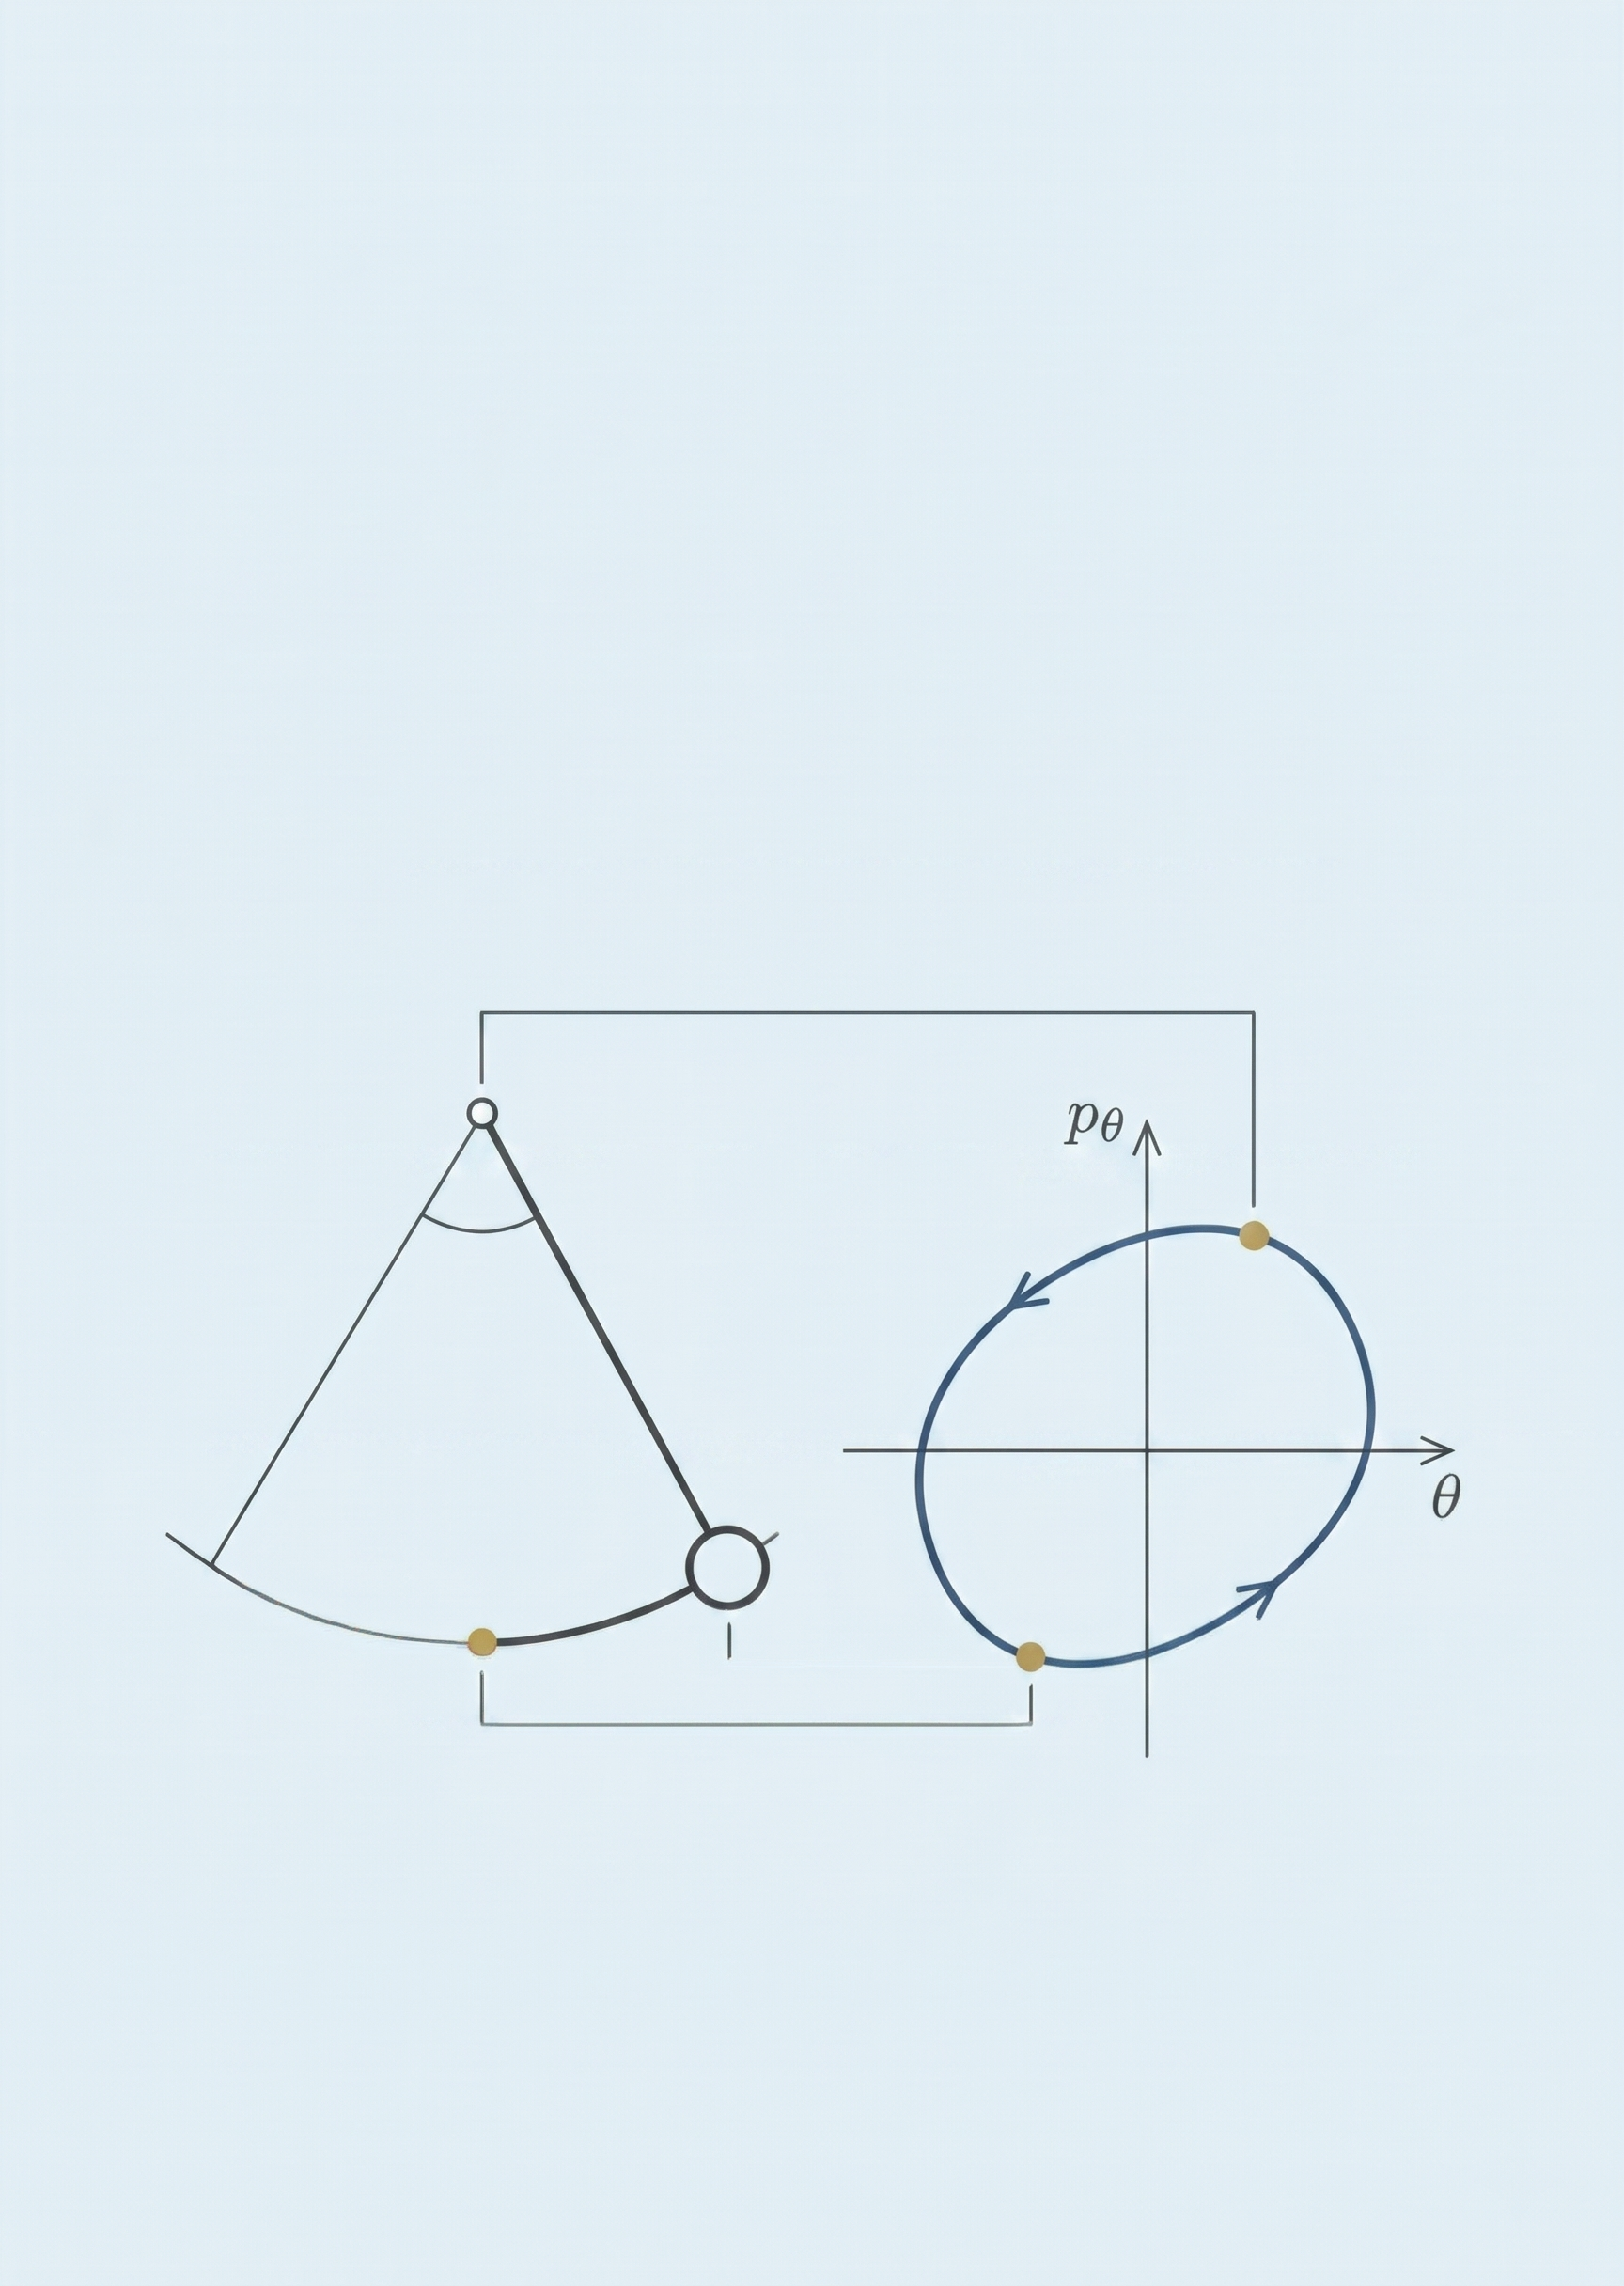
\includegraphics[height=\paperheight,keepaspectratio]{../../../generated_course_notes/core/classical_mechanics/2011_fall_theoretical_minimum/assets/cover-art.png}%
  };
  \node[
    anchor=north west,
    align=left,
    text width=0.78\paperwidth,
    fill=white,
    fill opacity=0.9,
    rounded corners=8pt,
    inner xsep=10pt,
    inner ysep=8pt
  ] at ([xshift=0.08\paperwidth,yshift=-0.06\paperheight]current page.north west) {%
    {\fontsize{30}{33}\selectfont\bfseries\color{black!88} 經典力學\\[0.85em]}
    {\large\color{black!72} 繁體中文版 / 2011年秋季・理論最低限度}
  };
  \node[
    anchor=south west,
    align=left,
    text width=0.68\paperwidth,
    fill=white,
    fill opacity=0.82,
    text opacity=1,
    rounded corners=6pt,
    inner sep=12pt
  ] at ([xshift=0.08\paperwidth,yshift=0.08\paperheight]current page.south west) {%
    {\normalsize\color{black!78} 原講授：Leonard Susskind\\[0.35em]}
    {\small\color{black!72} 講義輔助版本：\href{https://lazying.art}{LazyingArt LLC} / \href{https://github.com/lachlanchen/Video2Book}{Video2Book}}
  };
\end{tikzpicture}
\mbox{}
\end{titlepage}
\hypersetup{pageanchor=true}

\clearpage
\chapter*{關於這些筆記}
這些經過獨立編輯的配套筆記，依據 Leonard Susskind 的講課內容整理而成。筆記是根據機器轉錄稿、字幕及選定的黑板畫面重建，再與可取得的原始資料核對。這些筆記並非 Susskind 教授的原稿，也未經他審閱或認可。

本版由 \href{https://lazying.art}{LazyingArt LLC} 採用開源 \href{https://github.com/lachlanchen/Video2Book}{Video2Book} 工作流程編製。機器轉錄稿另行提供，其中可能有辨識錯誤。編輯上的補充說明及非平凡的重建均以腳註標示。
\clearpage
\tableofcontents
\mainmatter
\chapter{狀態、可逆性與運動學}

經典力學不只是一組描述落體、行星繞行或帶電粒子運動的方程式。在選定任何特定方程式之前，我們可以先提出一個更一般的問題：運動定律必須具備什麼形式，才算是經典定律？我們先從簡單到能把每一種可能歷程都畫在黑板上的系統談起。釐清其中的狀態、決定性、可逆性與守恆概念後，我們再回到普通空間中的粒子運動。

\section{兩類問題}

力學中的問題有兩類。一類是詢問支配特定系統的具體定律。行星在大質量物體的引力場中運動，遵循一種定律；帶電粒子在磁場中運動，則遵循另一種定律。這些問題關乎自然界的具體定律。

另一類問題關乎所有這些例子共有的架構。是否有某些規則是每一條容許的定律都必須遵守的？哪些特徵屬於經典力學本身，而與所研究的力或物體無關？具體例子能說明答案，但這門學科是由第二類問題組織起來的。

最適合用來入門的例子，是一枚放在抽象桌面上的抽象硬幣。我們只保留硬幣的一項性質：它可以呈現正面或反面。因此，它的構型空間是
\begin{equation}
  \mathcal C=\{H,T\}.
\end{equation}
「\emph{構型}」指的是系統可能呈現的狀態之一。初始條件就是選定其中一種狀態。單面硬幣會更簡單，但它只有一種構型，因此什麼都不會發生。兩種狀態就足以讓動力學成為可能。

\section{硬幣：狀態、定律與歷程}

讓時間以整數步進行，就像世界由頻閃燈照亮一樣：
\begin{equation}
  t=\ldots,-2,-1,0,1,2,\ldots .
\end{equation}
運動定律是一條更新規則，將時刻\(t\)的狀態指定為時刻\(t+1\)的狀態。最簡單的規則是保持原狀：
\begin{equation}
  H\longmapsto H,
  \qquad
  T\longmapsto T.
  \label{eq:coin-identity}
\end{equation}
從\(H\)出發，完整歷程是\(H,H,H,\ldots\)；從\(T\)出發，則是\(T,T,T,\ldots\)。這條規則雖然乏味，卻能完全預測後續狀態。

另一條可逆規則會交換這兩種狀態：
\begin{equation}
  H\longmapsto T,
  \qquad
  T\longmapsto H.
  \label{eq:coin-flip}
\end{equation}
現在，歷程會交替出現：
\begin{equation}
  H,T,H,T,\ldots,
  \qquad
  T,H,T,H,\ldots .
\end{equation}
箭頭由更新前的狀態指向更新後的狀態。因此，箭尾表示系統從哪個狀態出發，箭頭則表示它接著進入哪個狀態。

\begin{figure}[htbp]
  \centering
  \includegraphics[width=0.86\textwidth]{lecture_01_figure_02.png}
  \caption{硬幣的兩種構型，以及課堂黑板上的有向翻轉定律。清楚的更新規則見式~\eqref{eq:coin-flip}。}
  \lectureframe{00:06:50}
  \label{fig:coin-board}
\end{figure}

我們可以用一個二值變數來標記硬幣的兩面，
\begin{equation}
  \sigma=
  \begin{cases}
    +1,&H,\\
    -1,&T.
  \end{cases}
\end{equation}
物理學中常用字母\(\sigma\)表示二值量，特別是在描述自旋時；不過，這裡不需要任何自旋相關知識。用這套記號，兩條規則可寫成運動方程：
\begin{align}
  \sigma(t+1)&=\sigma(t),
  &&\text{identity law},\label{eq:sigma-identity}\\
  \sigma(t+1)&=-\sigma(t),
  &&\text{flip law}.\label{eq:sigma-flip}
\end{align}
這個變數沒有引入新的物理內容，只是為構型提供簡潔的標記，並將圖示改寫成方程式。

\begin{figure}[htbp]
  \centering
  \includegraphics[width=0.86\textwidth]{lecture_01_figure_03.png}
  \caption{翻轉定律寫成
  \(\sigma(t+1)=-\sigma(t)\)。方框中的數值\(\sigma=\pm1\)分別標記正面與反面。}
  \lectureframe{00:08:58}
  \label{fig:sigma-board}
\end{figure}

無論採用哪一條規則，初始狀態與定律都能決定之後每一時刻的狀態。這個說法假設系統是\emph{封閉}的。如果有人伸手進來轉動硬幣，那隻手就是未納入描述的外部影響。這並沒有推翻決定性；我們只是改變了所描述的系統。經典定律旨在支配封閉系統，並將所有會影響其演化的因素都納入考量。

從一個含有兩個元素的集合映射到自身，共有四種數學函數。上面未列出的兩種函數，會把兩個輸入都映至\(H\)，或都映至\(T\)。它們對未來的預測是確定的，卻抹去了兩種可能過去之間的差異。如下文所述，施加可逆性條件後，恰好只有式~\eqref{eq:coin-identity}與\eqref{eq:coin-flip}這兩種映射符合要求。

\section{骰子：軌道與守恆量}

把硬幣換成骰子。就目前的討論而言，骰子唯一重要的性質是它有六種構型，
\begin{equation}
  \mathcal C=\{1,2,3,4,5,6\}.
\end{equation}
初始條件就是選定其中一個數字。我們也可以再次讓每個狀態保持不變，但要描述較不平凡的規則，有向圖會更有用。考慮
\begin{equation}
  1\longmapsto2\longmapsto3\longmapsto4
  \longmapsto5\longmapsto6\longmapsto1.
  \label{eq:six-cycle}
\end{equation}
例如，從\(4\)出發的歷程是

\[
  4,5,6,1,2,3,4,\ldots .
\]
六個狀態構成一個迴圈。\footnote{來源註記：第一次依箭頭讀圖時，有一句口述說\(6\)會回到\(6\)。緊接著的說明、畫出的迴圈，以及列出的歷程，都表明預期的更新規則是\(6\mapsto1\)。}

\begin{figure}[htbp]
  \centering
  \includegraphics[width=0.86\textwidth]{lecture_01_figure_06.png}
  \caption{單一的六狀態迴圈。每經過一個頻閃時間步，狀態就移至下一個狀態；更新六次後便回到起點。}
  \lectureframe{00:12:40}
  \label{fig:six-cycle-board}
\end{figure}

規則看起來可以更複雜，結構上卻沒有不同。例如，
\begin{equation}
  1\to2\to5\to3\to4\to6\to1
  \label{eq:relabeled-cycle}
\end{equation}
仍然是一個六狀態迴圈。如果依照\(1,2,5,3,4,6\)的順序將頂點排列在頁面上，得到的圖就與式~\eqref{eq:six-cycle}相同。像\(1\)和\(5\)這樣的標記只是名稱；迴圈結構不受名稱影響。

另一條在結構上確實不同的定律，會把六個狀態分成兩個迴圈，例如
\begin{equation}
  1\to2\to3\to1,
  \qquad
  4\to6\to5\to4.
  \label{eq:two-cycles}
\end{equation}
系統仍然只有一顆骰子和一條定律，但從一個迴圈出發的軌跡永遠到不了另一個迴圈。我們可以為這些迴圈指定一個數值\(Q\)，
\begin{equation}
  Q=
  \begin{cases}
    0,&\text{on the cycle }\{1,2,3\},\\
    1,&\text{on the cycle }\{4,5,6\}.
  \end{cases}
\end{equation}
狀態每一步都會改變，但\(Q\)保持不變。

\begin{definition}
守恆量是狀態的一個函數，其值在運動定律作用下保持不變。
\end{definition}

同樣的想法也容許一個不動點、一個二狀態迴圈和一個三狀態迴圈。守恆標記指出系統位於哪條軌道上，不一定能辨別該軌道內的具體狀態。因此，守恆與運動並不矛盾。保持不變的未必是完整構型，也可以是不同可能構型之間的某種區別。

\begin{figure}[htbp]
  \centering
  \includegraphics[width=0.86\textwidth]{lecture_01_figure_07.png}
  \caption{黑板上有數個互不連通的迴圈：一個不動點、一個二狀態迴圈和一個三狀態迴圈。狀態沿迴圈移動時，迴圈標記仍保持不變。}
  \lectureframe{00:18:40}
  \label{fig:conserved-cycles-board}
\end{figure}

對有限可逆系統而言，每條軌跡都是一個迴圈。單一迴圈不可能有這種簡單意義下的非定值守恆標記，因為軌跡最終會遍歷每個狀態。若有多個迴圈，則可以有這種標記，因為演化不會把狀態從一個部分帶到另一個部分。

\section{狀態必須包含哪些資訊？}

硬幣的例子採用一步規則：下一次呈現的面只取決於目前的面。聽眾提出的問題，正好用來檢驗這項限制是否不可或缺。

\begin{classroomqa}
\audiencequestion{能不能構造一串正面與反面的結果，使下一次的結果不只取決於眼前看得到的那一面，而是也取決於一個或幾個更早的結果？\lecturetimestamp{00:19:27--00:21:23}}

\lecturerresponse{可以。這種情況下，只有\(H\)或只有\(T\)都不是完整狀態。如果需要知道前一次呈現的面，就把狀態空間擴大為
\(
  \{HH,HT,TH,TT\}.
\)
每個有序對都記錄目前呈現的面和前一次呈現的面。如此一來，演化仍可寫成這個四狀態空間上的一步規則。如果還需要更多歷程資訊，也一併納入狀態。}
\end{classroomqa}

這個回答說明了狀態在實際操作上的意義。

\begin{definition}
系統在某一時刻的狀態，包含了所有必要資訊；這些資訊與運動定律合在一起，足以預測系統的未來。
\end{definition}

因此，狀態不只是一張快照，而是足以確定演化的完整資料。之後描述牛頓粒子時，光有位置並不足夠；速度也必須列入初始資料。帶有記憶的硬幣，是同一原理最簡單的例子。

\section{無限狀態空間}

狀態有無限多種，不代表需要無限多個物體。考慮一個粒子，它受限於無限直線上的整數格點。它的狀態是一個整數
\[
  n\in\mathbb Z.
\]
一條定律使它每一步向右移動一格：
\begin{equation}
  n(t+1)=n(t)+1.
  \label{eq:lattice-one}
\end{equation}
這條軌道永遠不會閉合，但若沿著未來和過去追蹤，就會經過每一個整數。就這個廣義而言，它扮演著一個無限延伸的迴圈。

另一條定律讓粒子每次移動兩格：
\begin{equation}
  n(t+1)=n(t)+2.
  \label{eq:lattice-two}
\end{equation}
此時偶數格點只會在偶數格點之間演化，奇數格點也只會在奇數格點之間演化。奇偶性守恆：
\begin{equation}
  \begin{aligned}
    Q_{\rm parity}(n)&=n\bmod 2,\\
    Q_{\rm parity}(n(t+1))&=Q_{\rm parity}(n(t)).
  \end{aligned}
\end{equation}
從有限構型空間轉為無限構型空間，雖然容許歷程永不重複，卻不會改變狀態、軌道或守恆的意義。

\section{有決定性仍不代表可逆}

現在來看一條能唯一預測未來，卻不符合另一項經典要求的規則。令一枚三面硬幣有正面、反面和邊緣三種狀態，並定義
\begin{equation}
  H\to T,
  \qquad
  T\to E,
  \qquad
  E\to T.
  \label{eq:nonreversible-map}
\end{equation}
從\(H\)出發，歷程是
\[
  H,T,E,T,E,\ldots;
\]
從\(T\)或\(E\)出發，之後的交替變化也同樣明確。每個狀態恰有一條出射箭頭，因此這條規則對未來具有決定性。

試圖重建過去時，問題就出現了。如果目前狀態是\(T\)，前一個狀態可能是\(H\)，也可能是\(E\)。兩條歷程合而為一。將所有箭頭反向，問題就一目了然：從\(T\)出發，反向圖有兩種可能的移動方式。反向規則不具決定性。

\begin{figure}[htbp]
  \centering
  \includegraphics[width=0.86\textwidth]{lecture_01_figure_08.png}
  \caption{不可逆的\(H,T,E\)定律與代表性歷程。
  \(H\)和\(E\)都匯入\(T\)，因此目前狀態無法唯一決定過去。}
  \lectureframe{00:28:50}
  \label{fig:nonreversible-board}
\end{figure}

\begin{definition}
若目前狀態能唯一決定下一個狀態，也能唯一決定前一個狀態，這條離散定律就是可逆的。在狀態圖中，每個狀態都必須恰有一條出射箭頭和一條入射箭頭。
\end{definition}

對有限狀態空間而言，可逆更新就是狀態的置換。它不會創造或消除狀態之間的差異，只會重新排列狀態。因此，它的圖會分解成數個迴圈。式~\eqref{eq:nonreversible-map}所示的映射雖然是函數，卻不是一對一函數，所以沒有反函數。

\begin{classroomqa}
\audiencequestion{如果這種規則描述的是粒子的機率，這樣的規則可以接受嗎？\lecturetimestamp{00:29:46--00:31:17}}

\lecturerresponse{那就屬於不同的架構。本文所述的基本經典力學採用確定性定律，而不是機率性的更新規則。當然可以自行提出並研究這類規則，但就這裡的意義而言，它不是經典力學定律。量子力學的決定方式不同，但仍有類似可逆演化的概念；這需要留待後續討論。經典統計力學也使用機率，但它以底層的力學定律為基礎，並用機率表示我們對初始資料所知不完整。}
\end{classroomqa}

這項區別很重要。若因為不知道確切的經典狀態而使用機率分布，它就不是非決定性的運動定律。機率分布描述的是我們對系統掌握的資訊；該系統的微觀演化仍假定具有決定性且可逆。

\section{精確定律與不完整的知識}

要作出預測，需要兩項要素：
\begin{enumerate}
  \item 運動定律；
  \item 初始狀態。
\end{enumerate}
若初始條件只知道大約值，精確定律也無法給出精確預測。對硬幣來說，要想像看一眼桌面便完全知道它呈現哪一面，並不困難。真實的力學變數是連續的；位置和速度可以取任意實數值，而測量無法提供無限多位小數。

假設真實的初始狀態落在一小片可能狀態的範圍內。在某些動力學下，這片範圍會長時間維持得很小；在另一些動力學下，彼此接近的初始狀態則會迅速分開。在混沌系統中，微小的初始不確定性最終會擴大成顯著差異。大氣就是熟悉的例子。更精確的測量可以延長預測仍有用的時間，但無論測量精度固定為何，總會有某個足夠遙遠的時刻，使預測變得不可靠。

這項實際限制不會使方程產生歧義。若初始條件已知得精確，經典可逆定律便能決定未來與過去。若只能以有限精度掌握初始狀態，定量上要問的則是：若要預測指定長度的時間，初始狀態必須知道得多精確？

圖示檢驗現在可以簡潔地總結：若每個狀態都恰有一條入射箭頭和一條出射箭頭，所表示的定律就具有決定性且可逆。套用到粒子的相應說法會比較不簡單，但表達的是同一種經典架構。

\section{從抽象狀態到空間中的點}

接下來，我們從硬幣和骰子轉向點粒子。粒子可以在一維、三維、五維或任意其他維度中運動；普通空間是最直接的例子。若要定量描述一個點，必須選定：
\begin{itemize}
  \item 一個原點；
  \item 三條彼此垂直的座標軸；
  \item 這些座標軸的取向；
  \item 一個長度單位。
\end{itemize}
原點的位置是任意約定的，可以設在帕羅奧圖或其他任何地方；物理結論不應取決於這項選擇。座標軸可以標記為\(x,y,z\)，或\(x_1,x_2,x_3\)。確定\(x\)與\(y\)方向後，\(z\)軸仍可指向兩個互相垂直方向中的任一個。我們採用右手定則：右手拇指沿\(x\)方向、食指沿\(y\)方向時，中指便指向\(z\)方向。

座標軸上等距的刻度需要指定長度單位，例如公尺、英尺、英吋或光年。這些約定確定後，每個點便以三個數標記，
\begin{equation}
  (x,y,z).
\end{equation}
從原點沿三條座標軸移動，就可以到達該點。多粒子系統中的每個粒子，都需要一組這樣的三個座標。

\begin{figure}[htbp]
  \centering
  \includegraphics[width=0.86\textwidth]{lecture_01_figure_09.png}
  \caption{笛卡兒座標軸與一個點的三個座標。圖中採用一套座標約定；點本身則不受原點或座標軸的位置選擇影響。}
  \lectureframe{00:43:00}
  \label{fig:coordinates-board}
\end{figure}

\section{向量及其分量}

向量是具有大小與方向的量。從原點指向某一點的位移是一個向量；速度、加速度、電場及許多其他物理量也都可以用向量描述。我們以粗體表示向量，例如\(\mathbf v\)；其大小則記為\(\lvert\mathbf v\rvert\)。向量大小必為非負數，且只有零向量的大小為零。

從幾何上看，向量是一支可以自由平移的箭頭。只要長度和方向不變，平移箭頭並不會改變向量。在特定應用中，向量可以附著於某個點，例如指定某位置的電場；但附著位置是額外資訊，並非抽象向量本身的一部分。

相對於笛卡兒座標軸，向量的分量為
\begin{equation}
  \mathbf v=(v_x,v_y,v_z).
\end{equation}
分量是帶正負號的普通數值，可由向量在各軸上的投影得到；它們共同編碼了向量的大小與方向。三維勾股定理給出
\begin{equation}
  \lvert\mathbf v\rvert^2
  =v_x^2+v_y^2+v_z^2,
  \qquad
  \lvert\mathbf v\rvert
  =\sqrt{v_x^2+v_y^2+v_z^2}.
  \label{eq:vector-magnitude}
\end{equation}
分量的比例決定方向。分量為負，表示向量有一部分指向該座標軸的負向。

\subsection{純量乘法與向量加法}

以實數乘向量會改變向量的長度；若該實數為負，方向也會反轉。當\(c>0\)時，\(c\mathbf A\)與\(\mathbf A\)同向，大小為
\(c\lvert\mathbf A\rvert\)。特別是，\(-\mathbf A\)與\(\mathbf A\)長度相同，但方向相反。

向量加法有三種等價的圖示方式。第一種，將\(\mathbf B\)的箭尾放在\(\mathbf A\)的箭頭處；從\(\mathbf A\)的箭尾指向\(\mathbf B\)的箭頭之向量，就是\(\mathbf A+\mathbf B\)。
第二種，讓兩個向量的箭尾重合，再補成平行四邊形；其對角線就是兩向量的和。這種畫法清楚呈現交換律：
\begin{equation}
  \mathbf A+\mathbf B=\mathbf B+\mathbf A.
\end{equation}
第三種，將對應的分量相加：
\begin{equation}
  C_i=A_i+B_i,
  \qquad i=x,y,z,
  \label{eq:component-addition}
\end{equation}
其中\(\mathbf C=\mathbf A+\mathbf B\)。這些規則也定義了\(a\mathbf A+b\mathbf B\)等一般線性組合。

\begin{figure}[htbp]
  \centering
  \includegraphics[width=0.86\textwidth]{lecture_01_figure_10.png}
  \caption{向量加法的三角形與平行四邊形作圖法。兩種作圖法得到相同的向量\(\mathbf A+\mathbf B\)。}
  \lectureframe{00:53:00}
  \label{fig:vector-addition-board}
\end{figure}

一般而言，沒有將一個向量除以另一個向量的運算。不過，向量有兩種標準的乘積。叉積留待之後的課程討論；這裡需要介紹的是點積。

\subsection{點積}

將\(\mathbf A\)投影到由\(\mathbf B\)所定義的軸上。若兩向量的夾角為\(\theta\)，則\(\mathbf A\)沿\(\mathbf B\)方向的帶符號分量為\(\lvert\mathbf A\rvert\cos\theta\)。將這個投影乘以\(\lvert\mathbf B\rvert\)，便定義出
\begin{equation}
  \mathbf A\cdot\mathbf B
  =\lvert\mathbf A\rvert\,\lvert\mathbf B\rvert\cos\theta.
  \label{eq:dot-geometric}
\end{equation}
結果是純量，不是另一個向量。式~\eqref{eq:dot-geometric}對\(\mathbf A\)和\(\mathbf B\)是對稱的，因此\(\mathbf A\cdot\mathbf B=\mathbf B\cdot\mathbf A\)。

\begin{figure}[htbp]
  \centering
  \includegraphics[width=0.86\textwidth]{lecture_01_figure_11.png}
  \caption{黑板上利用投影來構造點積。
  排版後的形式為
  \(\mathbf A\cdot\mathbf B=AB\cos\theta\)。}
  \lectureframe{00:58:30}
  \label{fig:dot-product-board}
\end{figure}

點積的正負號包含幾何資訊：兩向量夾銳角時為正，夾鈍角時為負，彼此垂直時為零。因此，對非零向量而言，
\begin{equation}
  \mathbf A\perp\mathbf B
  \quad\Longleftrightarrow\quad
  \mathbf A\cdot\mathbf B=0
\end{equation}

用分量表示，
\begin{equation}
  \mathbf A\cdot\mathbf B
  =A_xB_x+A_yB_y+A_zB_z.
  \label{eq:dot-components}
\end{equation}
這個公式讓計算變得直接。特別是，
\begin{equation}
  \mathbf A\cdot\mathbf A
  =A_x^2+A_y^2+A_z^2
  =\lvert\mathbf A\rvert^2.
  \label{eq:self-dot}
\end{equation}
給定兩向量的分量後，利用式~\eqref{eq:dot-geometric}與\eqref{eq:dot-components}即可求出它們的夾角：
\begin{equation}
  \cos\theta
  =\frac{\mathbf A\cdot\mathbf B}
  {\lvert\mathbf A\rvert\,\lvert\mathbf B\rvert}.
\end{equation}

餘弦定理可由相同的代數運算推得。令\(\mathbf A\)和\(\mathbf B\)從同一頂點指向三角形的另外兩個頂點。第三邊的向量是\(\mathbf C=\mathbf A-\mathbf B\)，而不是\(\mathbf A+\mathbf B\)。因此
\begin{align}
  C^2
  &=(\mathbf A-\mathbf B)\cdot(\mathbf A-\mathbf B)\notag\\
  &=A^2+B^2-2\mathbf A\cdot\mathbf B\notag\\
  &=A^2+B^2-2AB\cos\theta.
  \label{eq:law-of-cosines}
\end{align}

\begin{figure}[htbp]
  \centering
  \includegraphics[width=0.86\textwidth]{lecture_01_figure_04.png}
  \caption{餘弦定理所用的三角形。黑板上的修正指出，閉合邊應為
  \(\mathbf C=\mathbf A-\mathbf B\)，由此得到式~\eqref{eq:law-of-cosines}。}
  \lectureframe{01:04:29}
  \label{fig:law-cosines-board}
\end{figure}

\section{位置、速度與加速度}

選定一個原點，令\(\mathbf r\)為從原點指向粒子的位置向量。它的分量就是笛卡兒座標：
\begin{equation}
  \mathbf r=(x,y,z),
  \qquad
  \lvert\mathbf r\rvert=\sqrt{x^2+y^2+z^2}.
\end{equation}
改變原點會改變\(\mathbf r\)，這個問題留待之後討論。原點一旦固定，便可用隨時間變化的位置描述運動：
\begin{equation}
  \mathbf r(t)=\bigl(x(t),y(t),z(t)\bigr).
\end{equation}
因此，軌跡可由三個時間函數表示。

速度是位置對時間的導數：
\begin{equation}
  \mathbf v(t)=\frac{d\mathbf r}{dt}
  =\dot{\mathbf r}(t),
  \qquad
  v_i=\frac{dx_i}{dt}=\dot x_i.
  \label{eq:velocity}
\end{equation}
點號一律表示對時間微分。\(\lvert\mathbf v\rvert\)的大小就是速率。一般而言，位置與速度的方向彼此獨立：粒子位於某處時，可以沿問題所容許的任意方向運動。

加速度是速度的變化率，因此也是位置對時間的二階導數：
\begin{equation}
  \mathbf a(t)=\frac{d\mathbf v}{dt}
  =\dot{\mathbf v}(t)
  =\frac{d^2\mathbf r}{dt^2}
  =\ddot{\mathbf r}(t),
  \qquad
  a_i=\ddot x_i.
  \label{eq:acceleration}
\end{equation}
加速度也是向量。若粒子沿\(x\)正向運動且速度增加，則\(a_x>0\)；若速度減小，則\(a_x<0\)。所謂減速度，就是方向與當前速度相反的加速度。更一般地說，即使速度大小不變，速度也可以因方向改變而改變。

\begin{figure}[htbp]
  \centering
  \includegraphics[width=0.86\textwidth]{lecture_01_figure_05.png}
  \caption{速度分量以位置分量對時間的導數表示。用簡潔的向量記號寫成
  \(\mathbf v=d\mathbf r/dt\)。}
  \lectureframe{01:14:24}
  \label{fig:velocity-board}
\end{figure}

\subsection{直線上的等加速度運動}

對一維運動，令
\begin{equation}
  x(t)=a+bt+ct^2.
  \label{eq:quadratic-motion}
\end{equation}
在\(t=0\)時，粒子位於\(x=a\)。先微分一次，再微分一次，可得
\begin{align}
  v(t)=\dot x(t)&=b+2ct,\label{eq:line-velocity}\\
  a(t)=\ddot x(t)&=2c.\label{eq:line-acceleration}
\end{align}
因此，\(b\)是初速度，\(2c\)是固定加速度。若\(c>0\)，速度便線性增加；若\(c<0\)，速度則線性減少。這種位置的二次函數形式，正是等加速度運動的特徵，例如地球表面附近落體運動的理想化描述。

\section{等速率圓周運動}

最後看一個例子：令粒子在\(x\)-\(y\)平面內沿單位圓運動。它在\(t=0\)時從\(x\)軸正向出發，角座標均勻增加：
\begin{equation}
  \theta(t)=\omega t.
\end{equation}
常數\(\omega\)稱為角頻率。角度增加\(2\pi\)就代表轉完一圈，因此週期為
\begin{equation}
  T=\frac{2\pi}{\omega}.
  \label{eq:circular-period}
\end{equation}
角度可以持續增加，超過\(2\pi\)；即使角度不歸零，位置仍會週期性重複。

在單位圓上，
\begin{equation}
  \mathbf r(t)
  =\bigl(\cos\omega t,\,\sin\omega t\bigr).
  \label{eq:circular-position}
\end{equation}
微分後可得
\begin{equation}
  \mathbf v(t)
  =\omega\bigl(-\sin\omega t,\,\cos\omega t\bigr).
  \label{eq:circular-velocity}
\end{equation}
速度與圓相切。我們不必依賴圖示，也能證明速度垂直於半徑：
\begin{align}
  \mathbf r\cdot\mathbf v
  &=\cos\omega t\,(-\omega\sin\omega t)
    +\sin\omega t\,(\omega\cos\omega t)\notag\\
  &=0.
  \label{eq:r-dot-v}
\end{align}

\begin{figure}[htbp]
  \centering
  \includegraphics[width=0.86\textwidth]{lecture_01_figure_12.png}
  \caption{粒子沿單位圓運動時的位置與速度分量。
  \(\mathbf r\cdot\mathbf v\)中的相消證明速度與圓相切。}
  \lectureframe{01:24:30}
  \label{fig:circular-velocity-board}
\end{figure}

再微分一次，
\begin{equation}
  \mathbf a(t)
  =-\omega^2
  \bigl(\cos\omega t,\,\sin\omega t\bigr)
  =-\omega^2\mathbf r(t).
  \label{eq:centripetal-acceleration}
\end{equation}
加速度與半徑平行，但方向相反，指向圓心。這就是向心加速度。\footnote{術語註記：講課在此處用了「``離心''」一詞，但方程式及其附帶說明所指的是標準的向心加速度，方向朝向圓心。}

\begin{figure}[H]
  \centering
  \includegraphics[width=0.86\textwidth]{lecture_01_figure_13.png}
  \caption{圓周運動的加速度分量計算。每個分量都是對應位置分量的\(-\omega^2\)倍，因此
  \(\mathbf a=-\omega^2\mathbf r\)。}
  \lectureframe{01:26:30}
  \label{fig:circular-acceleration-board}
\end{figure}

因為半徑為一，
\begin{equation}
  \lvert\mathbf r\rvert=1,
  \qquad
  \lvert\mathbf v\rvert=\omega,
  \qquad
  \lvert\mathbf a\rvert=\omega^2.
\end{equation}
增加\(\omega\)會使速率按比例增加，而所需的向內加速度則按平方增加。若圓的半徑為\(R\)，同樣的計算會得到\(v=\omega R\)和\(\lvert\mathbf a\rvert=\omega^2R=v^2/R\)；課堂上採用\(R=1\)，是為了讓第一次計算更簡潔。

現在，我們已具備粒子力學所需的基本語言：狀態與初始資料、可逆演化、座標、向量，以及定義速度與加速度的導數。接下來要確切判定，哪些初始資料足以指定一個粒子的狀態，並找出能將這些資料從一個時刻演化到下一個時刻的定律。
\chapter{力、相空間與守恆定律}

\lectureoverview{運動定律不能只把熟悉的物理量彼此聯繫起來。它還必須指定系統的狀態，描述該狀態如何從一個時刻演變到下一個時刻，並揭示運動過程中哪些區別與物理量得以保留。我們將先檢驗一條看似合理、實則錯誤的力定律，再將狀態從位置擴展到相空間，最後推導動量守恆與能量守恆。}

\section{一條有用的錯誤定律}

日常生活中的運動主要受摩擦影響。推一個重物在地板上移動，它就會動；停止推動後，它很快就停下來。通常推力越大，速度也越大；物體越重，所需的推力也越大。在這樣的世界裡，人們自然會認為力直接產生速度。亞里斯多德對運動的描述，基本上就是建立在這種直覺之上。

滑冰提供了缺少的經驗。滑冰者需要施力才能起步、停止或改變方向，但開始滑行後，若要繼續滑行，就不需要持續施力。假如亞里斯多德研究的是近乎無摩擦的冰面，而不是一般地面，那麼力--速度這種直覺的缺陷就很難不被察覺。

為了揭示這種直覺的問題，讓我們用現代方式將它寫成精確的形式。我們寫下這條刻意設為錯誤的方程：

\begin{equation}
  \mathbf F=m\mathbf v.
  \label{eq:aristotle-vector-law}
\end{equation}

這不是牛頓定律，不應把它當成物理定律來記憶。它的價值在於診斷問題：一旦把文字規則寫成方程，我們就能檢驗它是否能預測運動，以及是否保留足夠的資訊來重建過去。課堂上簡短談到希臘語中表示力的詞時，提到的是\emph{dynamis}；dynamo 和 dynamics 等詞也源自同一詞根。不過，相較於檢驗定律本身，這些術語並非重點。

\begin{figure}[htbp]
  \centering
  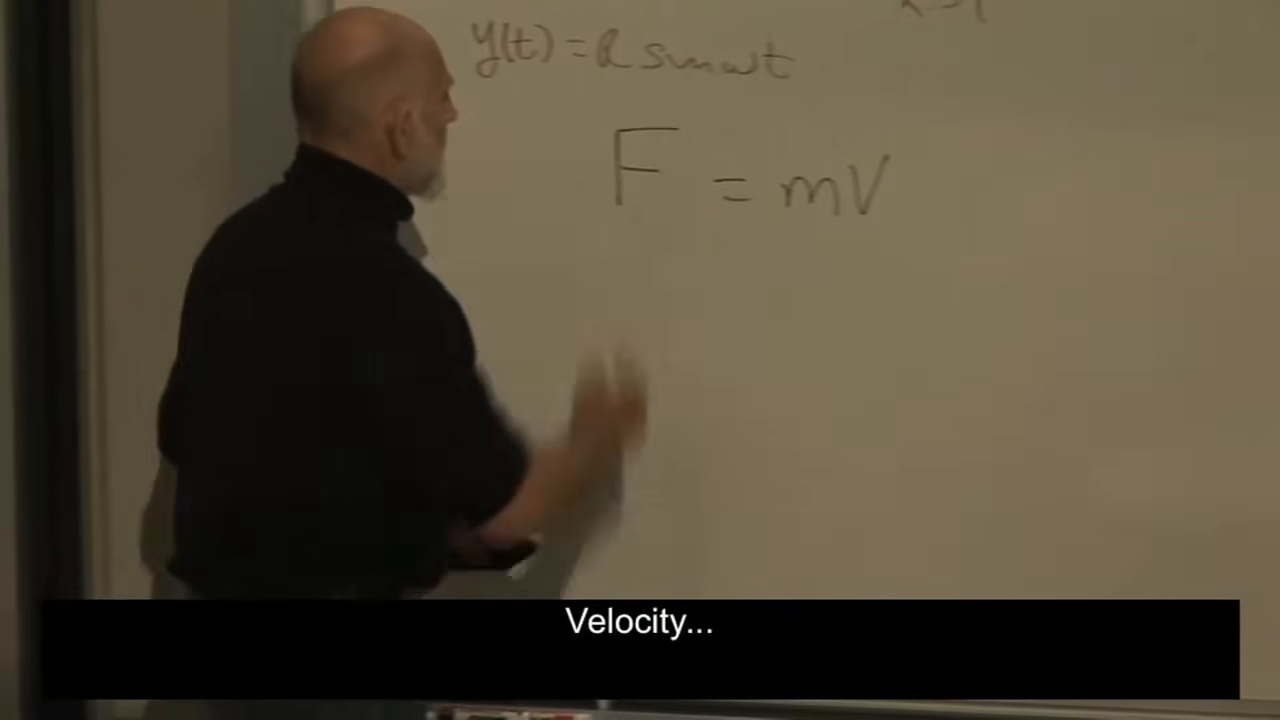
\includegraphics[width=0.82\textwidth]{lecture_02_figure_02.png}
  \caption{用來檢驗可預測性與可逆性的錯誤力--速度定律。}
  \lectureframe{00:04:51}
\end{figure}

將運動限制在一個空間座標上。由於 \(v=\dot x\)，這條定律可寫成

\begin{equation}
  F(t)=m\dot x(t).
  \label{eq:aristotle-1d}
\end{equation}

現在將時間分成長度為 \(\delta\) 的短區間。在一個區間內，

\begin{equation}
  \dot x(t)\simeq
  \frac{x(t+\delta)-x(t)}{\delta}.
  \label{eq:first-difference}
\end{equation}

將結果代入式~\eqref{eq:aristotle-1d}，得到

\begin{equation}
  x(t+\delta)
  =x(t)+\frac{\delta}{m}F(t).
  \label{eq:aristotle-update}
\end{equation}

這看起來像一條真正的更新規則：只要知道目前的位置和力，就能得出下一個頻閃時刻的位置。然而，當力為零時，亞里斯多德的規則給出 \(\dot x=0\)：物體必須維持靜止。從一開始，沒有持續施力就能保持運動的可能性便被排除在外。

\begin{figure}[htbp]
  \centering
  \includegraphics[width=0.84\textwidth]{lecture_02_figure_07.png}
  \caption{帶有恢復力的離散亞里斯多德更新。每一步都會將位移乘以略小於一的因子。}
  \lectureframe{00:10:15}
\end{figure}

\subsection{亞里斯多德力學中的彈簧}

考慮一個連接在彈簧上的粒子，其平衡位置為 \(x=0\)。粒子位移時，會受到恢復力

\begin{equation}
  F(x)=-kx,
  \qquad k>0.
  \label{eq:hooke-law}
\end{equation}

將這個力代入式~\eqref{eq:aristotle-update}，得到

\begin{equation}
  x(t+\delta)
  =\left(1-\frac{k\delta}{m}\right)x(t).
  \label{eq:aristotle-spring-update}
\end{equation}

當 \(\delta\) 足夠小時，括號中的因子略小於一。因此，每次更新都會以相同比例縮小位移：

\begin{equation}
  x_n=\left(1-\frac{k\delta}{m}\right)^n x_0.
  \label{eq:aristotle-geometric-decay}
\end{equation}

相應的連續方程及其解為

\begin{align}
  m\dot x&=-kx,
  \label{eq:aristotle-spring-continuous}\\
  x(t)&=x(0)e^{-kt/m}.
  \label{eq:aristotle-spring-solution}
\end{align}

彈簧不會振盪。粒子從任意位移處釋放後，都會以指數方式趨近原點，且越接近原點，移動得越慢。

\begin{figure}[htbp]
  \centering
  \includegraphics[width=0.84\textwidth]{lecture_02_figure_08.png}
  \caption{亞里斯多德彈簧方程的指數解。位移會衰減，而非振盪。}
  \lectureframe{00:12:02}
\end{figure}

未來很容易預測：無論初始位移為何，粒子都會趨近同一個靜止狀態。過去則是另一回事。假設我們只能以有限精度觀測到原點附近的粒子。它可能從許多不同的位移開始，因為這些位移留下的指數衰減殘量，最終都會小到落在同一個測量誤差範圍內。若有完美的數學精度，式~\eqref{eq:aristotle-spring-solution}可以反向求解；但在實際情況中，不同歷史之間的差異會逐漸被抹除。因此，從可逆的基礎動力學來看，這條定律令人起疑。

這不表示亞里斯多德的想法不合理。他描述的摩擦主導運動確實具有耗散性。問題在於，他把這種有效的描述提升為基本定律。摩擦本身也是一種力，來自複雜的微觀交互作用。手以大致固定的速度推動物體時，施力是在抵銷摩擦；施力本身並不是在產生速度。

\section{牛頓定律及其物理意義}

牛頓定律的修正之處在於：力會改變運動狀態：

\begin{equation}
  \mathbf F=m\mathbf a=m\ddot{\mathbf x}.
  \label{eq:newton-second-law}
\end{equation}

在將這條定律視為演化方程之前，必須先釐清兩個表面上的循環論證。第一個涉及參考系。人們常聽到，牛頓定律在慣性參考系中成立，而慣性參考系就是牛頓定律成立的參考系。但物理上的主張並不是這種循環定義，而是經驗性的：確實\emph{存在}某些參考系，可用適當的尺與鐘來描述，在這些參考系中，牛頓定律具有簡單的形式。相對於這些參考系加速或旋轉的參考系，則需要加入額外的表觀力。至於方程在其他參考系中如何變換，可以留待稍後推導。

第二個循環論證涉及力與質量。若把力定義為質量乘以加速度，又把質量定義為力除以加速度，這條方程看來就毫無內容。操作性實驗可以將定義與定律區分開來。先用天平讓物體與一公斤標準砝碼平衡，再在沒有其他力作用的空間中，將物體掛上彈簧秤。把彈簧固定的一小段伸長量定義為一單位的力。兩根相同的彈簧各自伸長相同的量，便提供兩單位的力，並產生兩倍的加速度。使用第二根彈簧比把一根彈簧拉長兩倍安全，因為真實的彈簧最後會進入非線性區域，甚至斷裂。若維持一根彈簧，改為連接兩個相同的質量，加速度就會減半；連接三個相同的質量，加速度則會變成三分之一。

\begin{figure}[htbp]
  \centering
  \includegraphics[width=0.84\textwidth]{lecture_02_figure_09.png}
  \caption{用來定義等量力單位並檢驗加速度與力成正比的彈簧秤思想實驗。}
  \lectureframe{00:22:45}
\end{figure}

這些比較讓下式具有經驗上的內容：

\begin{equation}
  a\propto F,
  \qquad
  a\propto\frac{1}{m},
  \qquad
  F=ma.
  \label{eq:force-mass-scaling}
\end{equation}

\emph{粒子}一詞在此泛指任何內部結構不重要的小物體，不限於基本粒子。

\subsection{為什麼單靠位置不足以描述狀態}

現在以同樣的頻閃方法檢驗牛頓方程。加速度的中心有限差分為

\begin{equation}
  \ddot x(t)\simeq
  \frac{x(t+\delta)-2x(t)+x(t-\delta)}{\delta^2}.
  \label{eq:second-difference}
\end{equation}

因此，牛頓方程意味著

\begin{equation}
  x(t+\delta)
  =2x(t)-x(t-\delta)+\frac{\delta^2}{m}F(t).
  \label{eq:newton-position-update}
\end{equation}

僅憑 \(x(t)\) 無法得出下一個位置。我們還需要前一個位置 \(x(t-\delta)\)，或等價地，需要目前時刻的速度。乍看之下，牛頓方程似乎不如亞里斯多德的方程具有預測性。正確的結論其實是：單靠位置不足以完整描述狀態。在某個時刻掌握所有相關資訊，意指掌握足以決定後續運動的資料。對牛頓力學中的粒子而言，這些資料就是位置與速度。

\section{動量與相空間}

定義動量如下：

\begin{equation}
  \mathbf p=m\mathbf v=m\dot{\mathbf x}.
  \label{eq:momentum-definition}
\end{equation}

對於固定的牛頓力學系統，質量視為常數。物體可能失去一部分，例如筆帽從筆上脫落；但此時描述的物體已經改變，而所選定的封閉系統仍有固定的總質量。當 \(m\) 保持不變時，牛頓第二定律可寫成

\begin{equation}
  \mathbf F=\dot{\mathbf p}.
  \label{eq:newton-momentum-form}
\end{equation}

\begin{figure}[htbp]
  \centering
  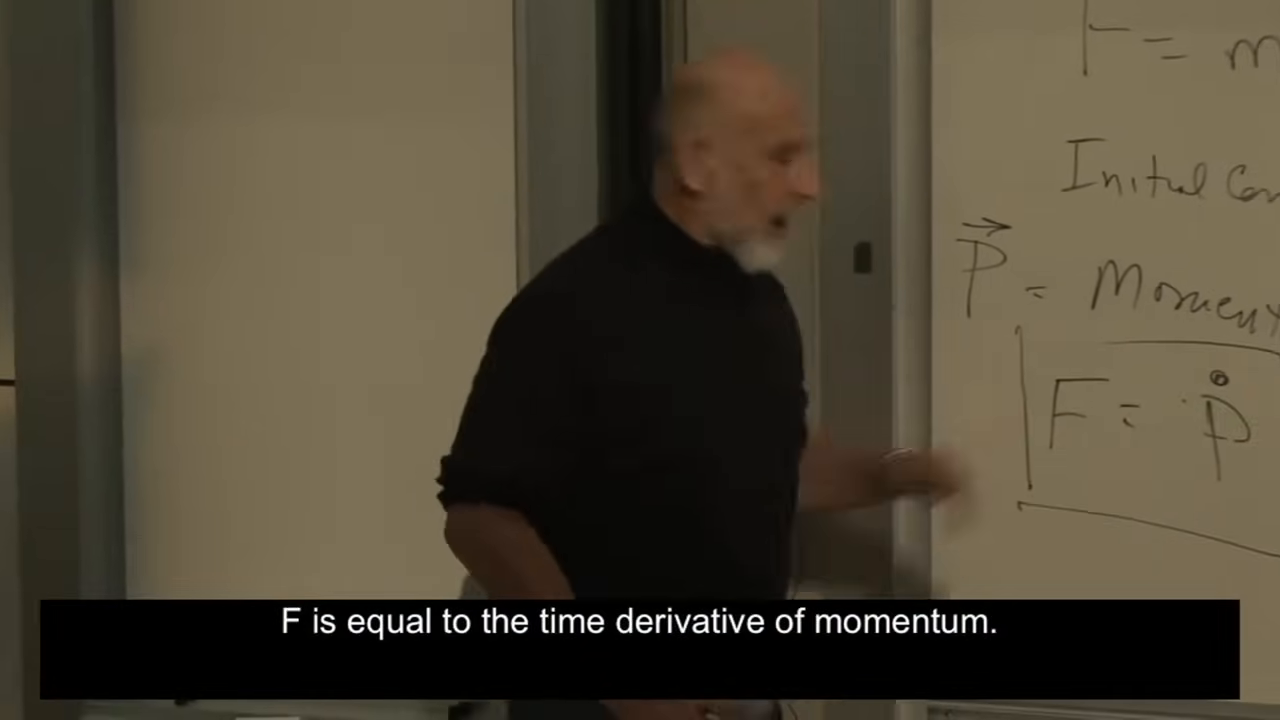
\includegraphics[width=0.82\textwidth]{lecture_02_figure_03.png}
  \caption{以動量對時間的導數表示的牛頓定律。}
  \lectureframe{00:32:35}
\end{figure}

對於一維運動，牛頓力學可寫成兩個關於兩個獨立狀態變數的一階方程：

\begin{align}
  \dot p&=F(x,t),
  \label{eq:first-order-p}\\
  \dot x&=\frac{p}{m}.
  \label{eq:first-order-x}
\end{align}

一個方程描述力如何改變動量；另一個描述動量如何改變位置。相應的一階離散形式為

\begin{align}
  p(t+\delta)&=p(t)+\delta F(x(t),t)+O(\delta^2),
  \label{eq:momentum-discrete}\\
  x(t+\delta)&=x(t)+\frac{\delta}{m}p(t)+O(\delta^2).
  \label{eq:position-discrete}
\end{align}

給定 \(x(t)\) 和 \(p(t)\) 後，這些方程便能決定下一組位置與動量；再將這組數值作為下一步的輸入。軌跡就是透過反覆更新建立起來的。

\begin{figure}[htbp]
  \centering
  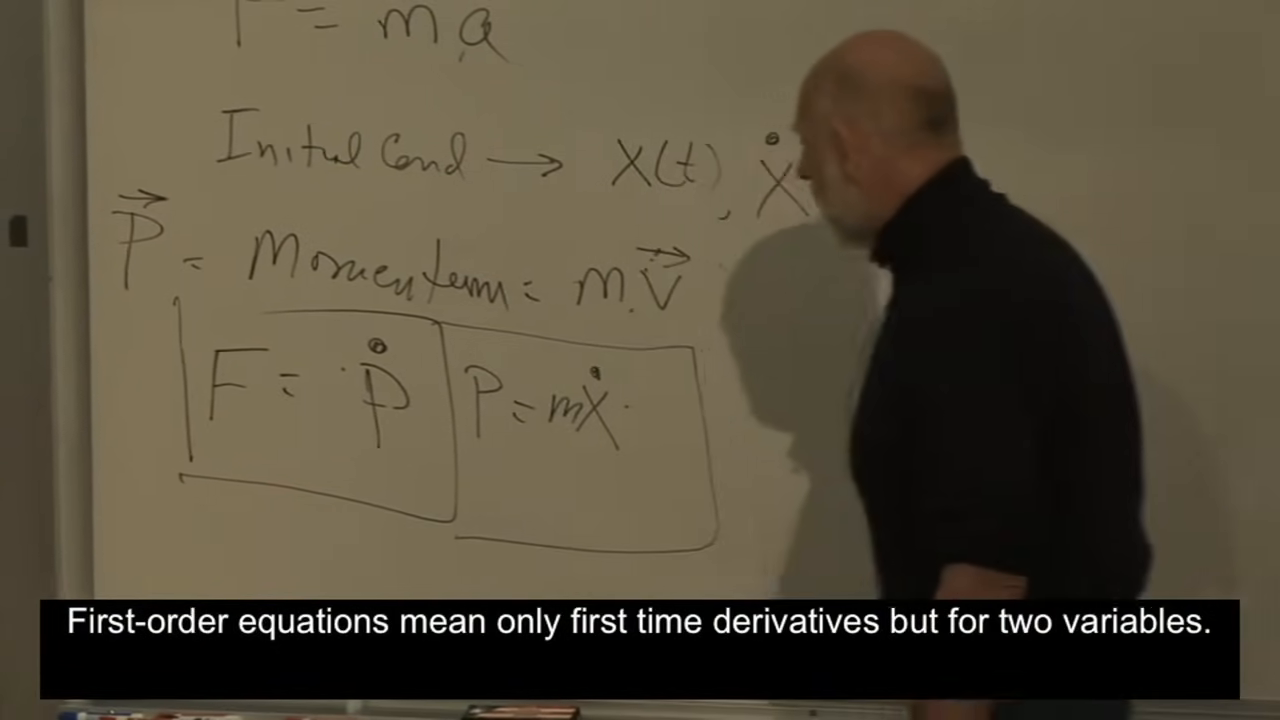
\includegraphics[width=0.84\textwidth]{lecture_02_figure_04.png}
  \caption{兩個一階方程及相應的初始資料。位置與動量合在一起指定系統的狀態。}
  \lectureframe{00:35:47}
\end{figure}

所有位置與動量配對 \((x,p)\) 所構成的空間稱為\emph{相空間}。對於在三維空間中運動的單一粒子，相空間有六個座標：

\begin{equation}
  (x,y,z,p_x,p_y,p_z).
  \label{eq:one-particle-phase-space}
\end{equation}

相空間是完整初始條件所構成的空間。位形空間只記錄位置；相空間則完整記錄運動定律所需的資料。

\begin{classroomqa}
  \audiencequestion{如果力是位置的函數，而不是已知的時間函數，更新過程會變得更複雜嗎？\lecturetimestamp{00:36:27--00:37:07}}
  \lecturerresponse{方程仍然具有預測性。一旦知道 \(x\) 和 \(p\)，就能得知 \(F(x)\) 的值。式~\eqref{eq:first-order-p}可推進 \(p\)，式~\eqref{eq:first-order-x}可推進 \(x\)，然後再次使用更新後的位置與動量。}
\end{classroomqa}

\section{牛頓力學中的彈簧}

回到彈簧問題，讓我們在相同的物理條件下比較這兩條定律。牛頓定律給出

\begin{equation}
  m\ddot x=-kx.
  \label{eq:newton-spring}
\end{equation}

暫時令 \(m=k=1\)，以消去常數。於是

\begin{equation}
  \ddot x=-x.
  \label{eq:normalized-oscillator}
\end{equation}

與指數函數不同，正弦或餘弦函數經過兩次微分後會變成自身的相反數。通解可以寫成

\begin{align}
  x(t)&=C\cos(t-t_0),
  \label{eq:oscillator-x}\\
  p(t)=\dot x(t)&=-C\sin(t-t_0).
  \label{eq:oscillator-p}
\end{align}

這兩個常數分別承載兩項初始資訊。振幅 \(C\) 給出最大位移，而 \(t_0\) 決定相位；這裡選擇相位，使粒子在 \(t=t_0\) 時速度為零。粒子只會在端點處短暫停止，接著便折返，經過原點時速率與動量最大，並繼續振盪。

將式~\eqref{eq:oscillator-x}和\eqref{eq:oscillator-p}平方，得到

\begin{equation}
  x^2+p^2=C^2.
  \label{eq:oscillator-phase-circle}
\end{equation}

因此，相空間中的點會沿半徑為 \(C\) 的圓移動。不同的初始振幅會對應到不同的圓；改變 \(t_0\)，則會在同一個圓上選擇不同的起點。在這些歸一化單位下，不論振幅為何，沿每個圓完成一周所需的週期都相同，為 \(2\pi\)。

\begin{figure}[htbp]
  \centering
  \includegraphics[width=0.84\textwidth]{lecture_02_figure_10.png}
  \caption{振子解及其在 \((x,p)\) 相平面中的圓形軌道。}
  \lectureframe{00:43:20}
\end{figure}

\begin{figure}[htbp]
  \centering
  \begin{tikzpicture}[scale=1.05,>=Latex]
    \draw[->] (-2.6,0) -- (2.75,0) node[right] {$x$};
    \draw[->] (0,-2.4) -- (0,2.55) node[above] {$p$};
    \draw[blue!65!black,thick] (0,0) circle (1.85);
    \draw[->,blue!65!black,thick]
      (1.60,0.93) arc[start angle=30,end angle=72,radius=1.85];
    \fill[red!65!black] (1.60,0.93) circle (2pt);
    \draw[dashed] (0,0) -- (1.60,0.93)
      node[midway,below right] {$C$};
    \node[align=left] at (-1.55,1.85)
      {$x=C\cos(t-t_0)$\\$p=-C\sin(t-t_0)$};
  \end{tikzpicture}
  \caption{相空間軌道同時保留位置與動量。半徑標示運動的振幅，而角度則隨時間均勻增加。}
  \label{fig:oscillator-phase-space}
\end{figure}

投影到水平軸上，得到 \(x\) 熟悉的往復運動；投影到垂直軸上，則得到 \(p\) 的振盪。亞里斯多德力學中的彈簧則不同：不同的圓不會彼此塌縮。知道相空間中的一點，就能決定系統的未來與過去。

對於一般的 \(m\) 與 \(k\)，角頻率為

\begin{equation}
  \omega=\sqrt{\frac{k}{m}},
  \qquad
  x(t)=C\cos\bigl(\omega(t-t_0)\bigr),
  \label{eq:general-oscillator-frequency}
\end{equation}

在未經縮放的 \((x,p)\) 平面中，相空間軌道會成為橢圓。講課中採用的 \(m=k=1\) 歸一化，則能方便地呈現圓形軌道。

\begin{classroomqa}
  \audiencequestion{如果把振子方程中的二階導數換成一階導數，是否就會失去可預測性？\lecturetimestamp{00:45:23--00:46:04}}
  \lecturerresponse{不會。給定適當的初始資料，一階方程仍可預測未來的運動。更深一層的問題是，方程所描述的流是否能充分保留不同狀態之間的差異，以維持可逆性。相關的一般定理，會等到具備所需的數學工具後再討論。}
\end{classroomqa}

\section{時間反演}

振子的圖像讓可逆性變得具體，但我們也可以直接檢驗方程。引入反向的時間座標

\begin{equation}
  T=-t.
  \label{eq:reverse-time}
\end{equation}

於是

\begin{equation}
  \frac{d}{dt}=-\frac{d}{dT},
  \qquad
  \frac{d^2}{dt^2}=\frac{d^2}{dT^2}.
  \label{eq:time-derivative-parity}
\end{equation}

時間反演會使一階導數變號，但不會改變二階導數。因此，自治的亞里斯多德方程

\begin{equation}
  m\dot x=F(x)
  \label{eq:aristotle-time-reversal}
\end{equation}

在影片倒放時不再具有相同形式。衰減的彈簧倒放後，會變成自行離開平衡位置的彈簧。相較之下，

\begin{equation}
  m\ddot x=F(x)
  \label{eq:newton-time-reversal}
\end{equation}

則維持原有形式。牛頓運動的影片倒放時，速度會反向，但加速度保持不變，因此倒放後的運動仍是方程允許的解。

\begin{figure}[htbp]
  \centering
  \includegraphics[width=0.84\textwidth]{lecture_02_figure_11.png}
  \caption{在 \(t\mapsto -t\) 變換下比較板書：一階導數變號，二階導數則不變。}
  \lectureframe{00:50:45}
\end{figure}

\begin{classroomqa}
  \audiencequestion{為什麼應將可逆性視為一般物理定律的前提？\lecturetimestamp{00:46:16--00:48:26}}
  \lecturerresponse{可逆性是經由檢驗而接受的，不是由定義保證的。我們考察成功的定律，找出它們共同的實驗特徵，再將這些特徵提升為原理。更深層的邏輯順序其實相反：量子場論更為基本，而牛頓力學則透過慢速運動、重物體等近似而出現。課程必須從較簡單的定律逐步建立，因此現在先將可逆性引入為一項原理，日後再檢驗它的適用範圍。}
\end{classroomqa}

\begin{classroomqa}
  \audiencequestion{牛頓是否曾有意識地將可逆性視為一個問題？\lecturetimestamp{00:48:28--00:49:02}}
  \lecturerresponse{歷史上的答案並不確定。牛頓確實理解慣性：改變運動狀態需要力，維持等速運動則不需要力。至於他是否曾明確地從可逆性的角度表述這項洞見，則是另一個歷史問題。}
\end{classroomqa}

\section{週期運動與守恆量}

相空間中的圓帶出下一個想法。軌跡始終留在同一個圓上，不會跳到另一個圓。因此，可以用一個沿運動保持不變的數值來標記這個圓。對於歸一化振子，這個數值是

\begin{equation}
  C^2=x^2+p^2.
  \label{eq:cycle-label}
\end{equation}

這就是振子的能量，相差一個二分之一的因子。半徑較大的圓具有較大的能量；改變起始相位並不會改變能量。我們會推導這個結論，而不是只從圖像中讀出來；不過，先來考慮動量。

牛頓第一定律指出，若物體所受合力為零，它就會以固定速度運動。這項定律已包含在第二定律中：

\begin{equation}
  \mathbf F=0
  \quad\Longrightarrow\quad
  \dot{\mathbf p}=0
  \quad\Longrightarrow\quad
  \mathbf v=\text{constant}
  \label{eq:newton-first-from-second}
\end{equation}

其中質量為常數。牛頓第三定律則提供了關於粒子間交互作用的真正新資訊。

\subsection{大小相等、方向相反且沿連心線的力}

令 \(\mathbf F_{ij}\) 表示粒子 \(i\) 受到粒子 \(j\) 施加的力。牛頓第三定律中大小相等、方向相反的部分是

\begin{equation}
  \mathbf F_{ij}=-\mathbf F_{ji}.
  \label{eq:newton-third-pair}
\end{equation}

如果這兩個力指向相同方向，一對孤立粒子就可能自發加速。這就成了不需要推進劑、只靠內力產生運動的機器；我們並未觀察到這種情形。

\begin{figure}[htbp]
  \centering
  \includegraphics[width=0.84\textwidth]{lecture_02_figure_12.png}
  \caption{以指標表示的交互作用力大小相等、方向相反關係。}
  \lectureframe{00:59:25}
\end{figure}

對於此處討論的點粒子力，這對作用力還沿著連接兩粒子中心的直線。如果大小相等、方向相反的力不在同一直線上，就可能形成純力矩，使一對孤立的剛體開始旋轉。沿連心線作用的條件排除了這種可能性：

\begin{equation}
  \mathbf F_{ij}\parallel
  (\mathbf r_i-\mathbf r_j).
  \label{eq:central-force-condition}
\end{equation}

大小相等、方向相反的條件將導出線動量守恆。沿連心線作用的條件則與角動量守恆有關，之後會再討論。

\begin{figure}[htbp]
  \centering
  \includegraphics[width=0.84\textwidth]{lecture_02_figure_13.png}
  \caption{牛頓第三定律中沿連心線作用的部分：交互作用力沿著連接兩粒子的直線作用。}
  \lectureframe{01:01:38}
\end{figure}

\subsection{總動量}

考慮一個包含 \(N\) 個粒子的封閉系統。系統沒有外力，只有粒子彼此施加的力。由力的可加性與牛頓第二定律可得，對每個粒子而言：

\begin{equation}
  \dot{\mathbf p}_i
  =m_i\ddot{\mathbf r}_i
  =\sum_{\substack{j=1\\j\ne i}}^N \mathbf F_{ij}.
  \label{eq:many-particle-newton}
\end{equation}

將此方程對 \(i\) 求和：

\begin{align}
  \frac{d}{dt}\sum_{i=1}^N\mathbf p_i
  &=\sum_{i=1}^N
    \sum_{\substack{j=1\\j\ne i}}^N\mathbf F_{ij}
  \notag\\
  &=\sum_{i<j}\bigl(\mathbf F_{ij}+\mathbf F_{ji}\bigr)
  =0.
  \label{eq:momentum-pair-cancellation}
\end{align}

每一組交互作用力都會出現兩次，分別代表作用力與反作用力，兩者相互抵銷。定義

\begin{equation}
  \mathbf P_{\mathrm{tot}}=\sum_{i=1}^N\mathbf p_i,
  \label{eq:total-momentum}
\end{equation}

便得到第一個守恆定律：

\begin{equation}
  \frac{d\mathbf P_{\mathrm{tot}}}{dt}=0.
  \label{eq:momentum-conservation}
\end{equation}

\begin{figure}[htbp]
  \centering
  \includegraphics[width=0.84\textwidth]{lecture_02_figure_14.png}
  \caption{將各粒子的方程相加後，成對的作用力會相互抵銷，留下總動量的時間導數為零。}
  \lectureframe{01:04:38}
\end{figure}

從歷史發展的角度來看，我們將動量守恆視為牛頓第三定律的推論。現代物理學往往把動量守恆看得更基本：如果一個孤立的雙粒子系統總動量守恆，內部動量的變化就必須大小相等、方向相反。不過，在目前的推導脈絡中，採用牛頓力學的推導方式較為合適。

\section{一維能量}

考慮一個粒子在直線上運動，所受的力只取決於位置：

\begin{equation}
  F=F(x).
  \label{eq:position-force}
\end{equation}

這種力稱為不顯含時間的力。這不表示運動中的粒子所受之力數值固定；力的數值會隨著 \(x(t)\) 改變。它的意思是，無論鐘錶顯示的時間為何，只要粒子位於相同位置 \(x\)，所受的力就相同。

在一維中，任何足夠平滑的力函數都可以積分。因此我們定義勢能 \(V(x)\) 如下：

\begin{equation}
  F(x)=-\frac{dV}{dx},
  \label{eq:potential-definition-1d}
\end{equation}

或等價地寫成

\begin{equation}
  V(x)=-\int^x F(u)\,du+V_0.
  \label{eq:potential-integral}
\end{equation}

加法常數 \(V_0\) 不會影響力。可以把 \(V(x)\) 想成 \(x\) 軸上方地形的高度。粒子會受到指向較低處的力，斜率越陡，力越大。在平滑山丘的頂端或底部，斜率為零，因此力也為零。

\begin{figure}[htbp]
  \centering
  \includegraphics[width=0.84\textwidth]{lecture_02_figure_15.png}
  \caption{以一維地形表示勢能。力指向下坡方向，大小由斜率決定。}
  \lectureframe{01:12:57}
\end{figure}

定義動能、勢能與總能量如下：

\begin{equation}
  T=\frac12m\dot x^2,
  \qquad
  E=T+V(x)
  =\frac12m\dot x^2+V(x).
  \label{eq:energy-1d}
\end{equation}

此時，能量只是我們給這個可能守恆的量取的名稱。地形圖提供了它的物理解釋：粒子往下移動時，\(V\) 會降低，速度則會增加，因此 \(T\) 也會增加；往上移動時則相反。牛頓方程可以證明，這兩者之間的轉換恰好相等。

對式~\eqref{eq:energy-1d}微分。由於 \(m\) 是常數，而 \(V\) 只透過 \(x(t)\) 隨時間改變，

\begin{align}
  \frac{dE}{dt}
  &=m\dot x\ddot x+\frac{dV}{dx}\dot x
  \notag\\
  &=\dot x\left(m\ddot x+\frac{dV}{dx}\right).
  \label{eq:energy-derivative-1d}
\end{align}

根據牛頓定律與 \(V\) 的定義，

\begin{equation}
  m\ddot x=F=-\frac{dV}{dx}.
  \label{eq:newton-potential-1d}
\end{equation}

因此，式~\eqref{eq:energy-derivative-1d}中的括號項為零：

\begin{equation}
  \frac{dE}{dt}=0.
  \label{eq:energy-conservation-1d}
\end{equation}

\begin{figure}[htbp]
  \centering
  \includegraphics[width=0.84\textwidth]{lecture_02_figure_16.png}
  \caption{一維能量的時間導數可寫成速度乘以牛頓方程。}
  \lectureframe{01:19:18}
\end{figure}

在一維中，只要力是足夠平滑且依賴位置，就不需要其他動力學假設，因為這類力都存在原函數。

\section{多維情形與保守力}

對於座標為 \(x_i\) 的粒子，牛頓方程的各分量為

\begin{equation}
  F_i(\mathbf x)=m\ddot x_i.
  \label{eq:newton-components}
\end{equation}

力的分量 \(F_i\) 可能取決於所有座標，而不只取決於 \(x_i\)。我們希望找到一個純量函數 \(V(\mathbf x)\)，使得

\begin{equation}
  F_i(\mathbf x)
  =-\frac{\partial V(\mathbf x)}{\partial x_i},
  \qquad
  \mathbf F=-\boldsymbol\nabla V.
  \label{eq:gradient-force}
\end{equation}

這不像一維的構造那樣必然成立。三個任意函數 \(F_1,F_2,F_3\) 通常包含比單一純量函數的各偏導數更多的獨立資訊。換句話說，只有在力場滿足相容條件時，才存在勢能；例如，相應的混合偏導數必須相等。在單連通區域中，這個條件可寫為 \(\boldsymbol\nabla\times\mathbf F=0\)。
因此，我們將式~\eqref{eq:gradient-force}視為適用於此處所討論力類別的物理假設，而非數學恆等式。

\begin{figure}[htbp]
  \centering
  \includegraphics[width=0.84\textwidth]{lecture_02_figure_17.png}
  \caption{多維力定律與勢能等高線示意圖。力穿過等高線，指向 \(V\) 減小的方向。}
  \lectureframe{01:24:15}
\end{figure}

在等高線圖上，\(V\)沿著每條等高線保持不變。梯度垂直於等高線，並指向上升最快的方向；力 \(-\boldsymbol\nabla V\) 則指向下降最快的方向。

\begin{figure}[htbp]
  \centering
  \begin{tikzpicture}[scale=1.0,>=Latex]
    \draw[->] (-3.0,0) -- (3.1,0) node[right] {$x_1$};
    \draw[->] (0,-2.4) -- (0,2.55) node[above] {$x_2$};
    \draw[orange!65!black,thick]
      plot[smooth cycle] coordinates
      {(-0.55,-0.35) (0.15,-0.55) (0.72,-0.10) (0.50,0.53) (-0.25,0.65)};
    \draw[orange!65!black,thick]
      plot[smooth cycle] coordinates
      {(-1.15,-0.75) (0.20,-1.10) (1.35,-0.25) (1.10,0.95) (-0.45,1.25)};
    \draw[orange!65!black,thick]
      plot[smooth cycle] coordinates
      {(-1.85,-1.20) (0.15,-1.70) (2.15,-0.40) (1.70,1.50) (-0.80,1.85)};
    \draw[->,blue!65!black,very thick] (1.62,0.73) -- (0.82,0.20)
      node[midway,above left] {$\mathbf F$};
    \draw[dashed,->,red!65!black,thick] (0.82,0.20) -- (1.62,0.73)
      node[midway,below right] {$\boldsymbol\nabla V$};
    \node[orange!65!black] at (-1.62,1.45) {$V=V_3$};
    \node[orange!65!black] at (-0.92,0.92) {$V=V_2$};
    \node[orange!65!black] at (-0.35,0.30) {$V=V_1$};
  \end{tikzpicture}
  \caption{純量勢的等高線。梯度垂直於等高線；保守力則指向相反方向。}
  \label{fig:potential-contours}
\end{figure}

若式~\eqref{eq:gradient-force}成立，定義

\begin{equation}
  E=\frac12m\sum_i\dot x_i^2+V(x_1,\ldots,x_n).
  \label{eq:energy-many-coordinates}
\end{equation}

動能項等於質量的一半乘以速度向量長度的平方。對其微分並使用多變數鏈鎖律，得到

\begin{align}
  \frac{dE}{dt}
  &=m\sum_i\dot x_i\ddot x_i
    +\sum_i\frac{\partial V}{\partial x_i}\dot x_i
  \notag\\
  &=\sum_i\dot x_i
    \left(m\ddot x_i+\frac{\partial V}{\partial x_i}\right)
  =0.
  \label{eq:energy-derivative-multidimensional}
\end{align}

這項證明與一維情形完全相同，只是多了指標；但前提更強：所有力分量都必須源自同一個勢能。

\begin{figure}[htbp]
  \centering
  \includegraphics[width=0.84\textwidth]{lecture_02_figure_18.png}
  \caption{帶有指標的能量導數。每個括號項都根據牛頓方程的相應分量而為零。}
  \lectureframe{01:28:30}
\end{figure}

對於三維空間中的 \(N\) 個粒子，將所有座標依序列出

\begin{equation}
  \begin{aligned}
    q_a={}&(x_1,y_1,z_1,x_2,y_2,z_2,\ldots,\\[-0.2em]
           &\phantom{(}x_N,y_N,z_N),\\
    &a=1,\ldots,3N.
  \end{aligned}
  \label{eq:flattened-coordinates}
\end{equation}

共有 \(3N\) 個座標分量，但只有 \(N\) 個粒子的質量；每個粒子的三個座標分量都使用同一個質量。若

\begin{equation}
  F_a=-\frac{\partial V(q_1,\ldots,q_{3N})}{\partial q_a},
  \label{eq:many-particle-conservative-force}
\end{equation}

則

\begin{equation}
  E=\sum_{A=1}^{N}\frac12m_A\lvert\dot{\mathbf r}_A\rvert^2
    +V(\mathbf r_1,\ldots,\mathbf r_N)
  \label{eq:many-particle-energy}
\end{equation}

根據相同的推導，這個量守恆。由勢能導出的力稱為\emph{保守}力，正是因為它們使這項守恆定律成立；這裡的「保守」一詞與政治立場無關。

\section{以能量等高線呈現的振子}
\enlargethispage{3\baselineskip}

對於彈簧力 \(F=-kx\)，由式~\eqref{eq:potential-definition-1d}可得

\begin{equation}
  V(x)=\frac12kx^2+V_0.
  \label{eq:spring-potential}
\end{equation}

選擇 \(V_0=0\) 後，振子的能量為

\begin{equation}
  E=\frac12m\dot x^2+\frac12kx^2
   =\frac{p^2}{2m}+\frac12kx^2.
  \label{eq:oscillator-energy}
\end{equation}

當 \(m=k=1\) 時，

\begin{equation}
  2E=p^2+x^2=C^2.
  \label{eq:oscillator-energy-circle}
\end{equation}

因此，先前得到的相空間圓就是等能線。對於更一般的一維勢能，等能線不一定是圓，但運動仍會沿著曲線進行：

\begin{equation}
  \frac{p^2}{2m}+V(x)=E
  \label{eq:general-energy-contour}
\end{equation}

曲線位於 \((x,p)\) 平面中。這讓我們回到第一講的想法：當軌跡始終留在彼此不同的週期軌道上時，可以用一個數值標記這些軌道，而且該數值在運動過程中保持不變。

現在我們已經有了狀態空間、牛頓力學的更新方程，以及前兩項守恆定律。接下來將介紹力學的另一種表述，從最小作用量原理出發，導向拉格朗日量、哈密頓量、角動量，以及這些例子背後更一般的結構。

\begin{classroomqa}
  \audiencequestion{發下來的講義和黑板上的內容有多一致？圖在哪裡？\lecturetimestamp{01:37:56--01:38:54}}
  \lecturerresponse{講義應該會緊跟課堂內容；如果黑板上的內容沒有收錄，可能是寄錯了檔案。圖還沒準備好；他開玩笑說，等繼續教育部門支付下一張支票時，圖就會出現。}
\end{classroomqa}
\chapter{駐定作用量與尤拉--拉格朗日方程}

\lectureoverview{熟悉的名稱\emph{最小作用量原理}掩蓋了關鍵之處：物理軌跡使作用量取駐值，但不一定使它取極小值。我們將從一般的平衡問題建立這個論述，將它從點推廣到整個函數，藉由離散化路徑推導尤拉--拉格朗日方程，並導出牛頓方程。接著，旋轉座標與極座標將說明，拉格朗日表述不只是改變記號而已。}

\section{取駐值，不一定取極小值}

傳統名稱中不可靠的是\emph{最小}一詞。經典軌跡不一定使作用量取極小值；在所有可能軌跡構成的空間中，它也可能對應極大值或鞍點。正確的原理是作用量\emph{取駐值}：它的一階變化為零。

先從較簡單的平衡問題談起。靜止不動的粒子沒有加速度，因此合力必須為零。若力來自一維勢能，
\begin{equation}
  F(x)=-\frac{dV}{dx},
  \label{eq:force-from-v}
\end{equation}
平衡條件就是
\begin{equation}
  \frac{dV}{dx}=0.
  \label{eq:stationary-v-one}
\end{equation}

\begin{figure}[htbp]
  \centering
  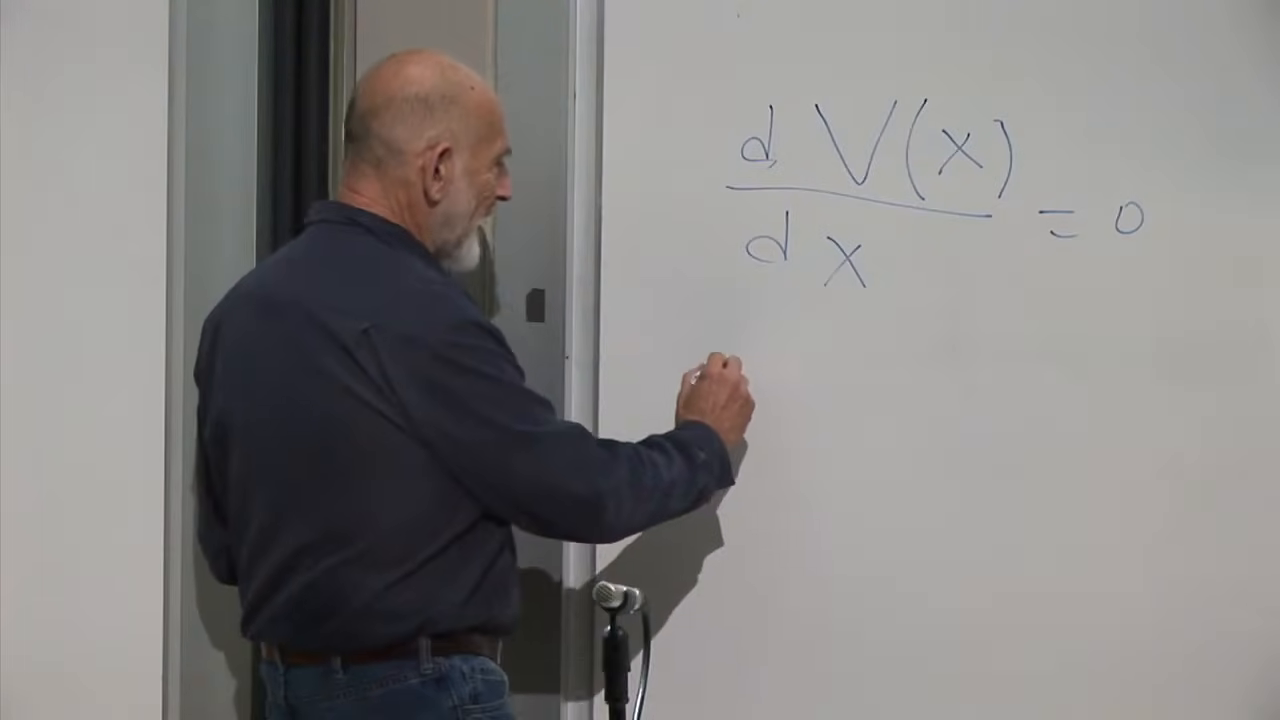
\includegraphics[width=0.74\textwidth]{lecture_03_figure_02.png}
  \caption{一維平衡條件：勢能取駐值處，力為零。}
  \lectureframe{00:02:51}
\end{figure}

現在讓粒子位移一小段\(\delta x\)。在一階近似下，
\begin{equation}
  \delta V
  =V(x+\delta x)-V(x)
  =\frac{dV}{dx}\,\delta x+O(\delta x^2).
  \label{eq:first-variation-one}
\end{equation}
在平衡位置，無論\(\delta x\)的正負為何，線性項都為零：
\begin{equation}
  \delta V=0
  \qquad\hbox{to first order.}
  \label{eq:delta-v-zero-one}
\end{equation}
這不表示有限位移後\(V\)完全不變，而是表示其主要變化從二階或更高階才開始。極小值和極大值都符合這個條件。

\begin{figure}[htbp]
  \centering
  \begin{tikzpicture}[scale=0.95,>=Latex]
    \draw[->] (-0.2,0) -- (3.35,0) node[right] {$x$};
    \draw[->] (0,-0.2) -- (0,2.25) node[above] {$V$};
    \draw[blue!65!black,thick,smooth]
      plot coordinates {(0.2,1.85) (0.75,0.85) (1.55,0.35)
                        (2.35,0.85) (3.0,1.85)};
    \fill[red!65!black] (1.55,0.35) circle (2pt);
    \node at (1.55,-0.34) {minimum};
    \begin{scope}[xshift=4.25cm]
      \draw[->] (-0.2,0) -- (3.35,0) node[right] {$x$};
      \draw[->] (0,-0.2) -- (0,2.25) node[above] {$V$};
      \draw[blue!65!black,thick,smooth]
        plot coordinates {(0.2,0.35) (0.75,1.25) (1.55,1.85)
                          (2.35,1.25) (3.0,0.35)};
      \fill[red!65!black] (1.55,1.85) circle (2pt);
      \node at (1.55,-0.34) {maximum};
    \end{scope}
  \end{tikzpicture}
  \caption{駐定條件決定一階導數，卻不能判定該點是極小值還是極大值。}
  \label{fig:min-max-stationary}
\end{figure}

對多個座標\(q_i\)而言，一階變分為
\begin{equation}
  \delta V
  =\sum_i\frac{\partial V}{\partial q_i}\,\delta q_i.
  \label{eq:first-variation-many}
\end{equation}
若此式必須對每一個彼此獨立的無窮小位移\(\delta q_i\)都為零，則每個係數都必須為零：
\begin{equation}
  \frac{\partial V}{\partial q_i}=0
  \qquad\hbox{for every }i.
  \label{eq:stationary-v-many}
\end{equation}

二維勢能不妨想成起伏的地形，而不是雲霄飛車的軌道。駐定點可能是谷底、山頂，也可能是鞍點。在鞍點附近，沿一個方向移動，勢能一開始會上升；沿另一個方向移動，勢能一開始則會下降。因此，恢復力在一個方向上可能穩定，在另一個方向上卻不穩定，儘管該點的所有一階導數都為零。

\begin{figure}[htbp]
  \centering
  \includegraphics[width=0.76\textwidth]{lecture_03_figure_06.png}
  \caption{鞍點沿所有方向的一階變化都為零，但沿一個軸向的鄰近位移會使勢能上升，沿另一個軸向的位移則會使勢能下降。}
  \lectureframe{00:08:20}
\end{figure}

在多座標構成的空間中，鞍點比單純的極大值或極小值更常見。因此，\emph{駐定}才是更恰當的用語。條件
\begin{equation}
  \delta V=0
  \label{eq:equilibrium-variation}
\end{equation}
概括了平衡狀態，卻不預先判定二階變化的性質。

\section{從點推廣到函數}

力學探討的是完整的運動，而非孤立的平衡點。軌跡是一個函數，例如\(x(t)\)，也可以由一組函數構成，例如\((x(t),y(t),z(t))\)。藉由改變整個函數，使某個量取駐值的數學方法稱為\emph{變分法}。在將變分法應用於運動之前，先看三個較簡單的例子。

\subsection{最短曲線與測地線}

在平面上固定兩點，並以\(y(x)\)表示兩點之間的一條曲線。對一小段曲線而言，
\begin{equation}
  ds=\sqrt{dx^2+dy^2}
  =dx\sqrt{1+\left(\frac{dy}{dx}\right)^2},
  \label{eq:line-element}
\end{equation}
最後一種寫法假設\(dx>0\)。整條曲線的長度是以下泛函：
\begin{equation}
  S[y]=\int_{x_0}^{x_1}
  \sqrt{1+y'(x)^2}\,dx.
  \label{eq:arc-length-functional}
\end{equation}
方括號表示\(S\)的輸入是整個函數。若曲線的小幅變化不改變兩端點，則滿足
\begin{equation}
  \delta S=0
  \label{eq:stationary-length}
\end{equation}
的曲線就是直線。

\begin{figure}[htbp]
  \centering
  \includegraphics[width=0.78\textwidth]{lecture_03_figure_07.png}
  \caption{兩個固定端點之間的一條試探曲線。曲線長度是各無窮小斜邊\(ds\)的總和。}
  \lectureframe{00:13:36}
\end{figure}

同樣的問題也可以在曲面上提出。把繩子在兩根樁之間拉緊，就能直觀呈現受限條件下的最短路徑。這種長度取駐值的曲線稱為\emph{測地線}。在平面上，測地線是直線；在球面或起伏的曲面上則通常不是。

\subsection{費馬原理}

在光速隨位置改變的介質中，光線\(c(x,y)\)不一定沿空間距離最短的路徑前進。光線通過一小段路徑所需的時間，是路段長度除以當地光速，因此
\begin{equation}
  T[y]
  =\int_{x_0}^{x_1}
  \frac{\sqrt{1+y'(x)^2}}{c(x,y)}\,dx.
  \label{eq:fermat-functional}
\end{equation}
費馬原理要求
\begin{equation}
  \delta T=0.
  \label{eq:fermat-stationary}
\end{equation}
當\(c\)為常數時，這就化為最短距離問題。但在折射率不均勻的介質中，最快的路徑必須兼顧路程長短與當地的傳播速度。

\begin{figure}[htbp]
  \centering
  \includegraphics[width=0.80\textwidth]{lecture_03_figure_08.png}
  \caption{光線在局部光速隨位置改變的介質中所需時間的泛函。}
  \lectureframe{00:22:50}
\end{figure}

一則應景的笑話提到當時新近出現的說法：中微子在義大利移動得異常快。物理論述隨即回到可靠的例子：普通光在物質中的速率會依折射率而改變。

\subsection{懸鏈}

兩端固定的鏈條會形成懸鏈線。鏈條的每一小段都貢獻重力位能，因此總位能本身就是沿鏈條積分所得。和前面的例子一樣，端點固定、未知形狀是一個函數，而某個積分必須取駐值。

\begin{figure}[htbp]
  \centering
  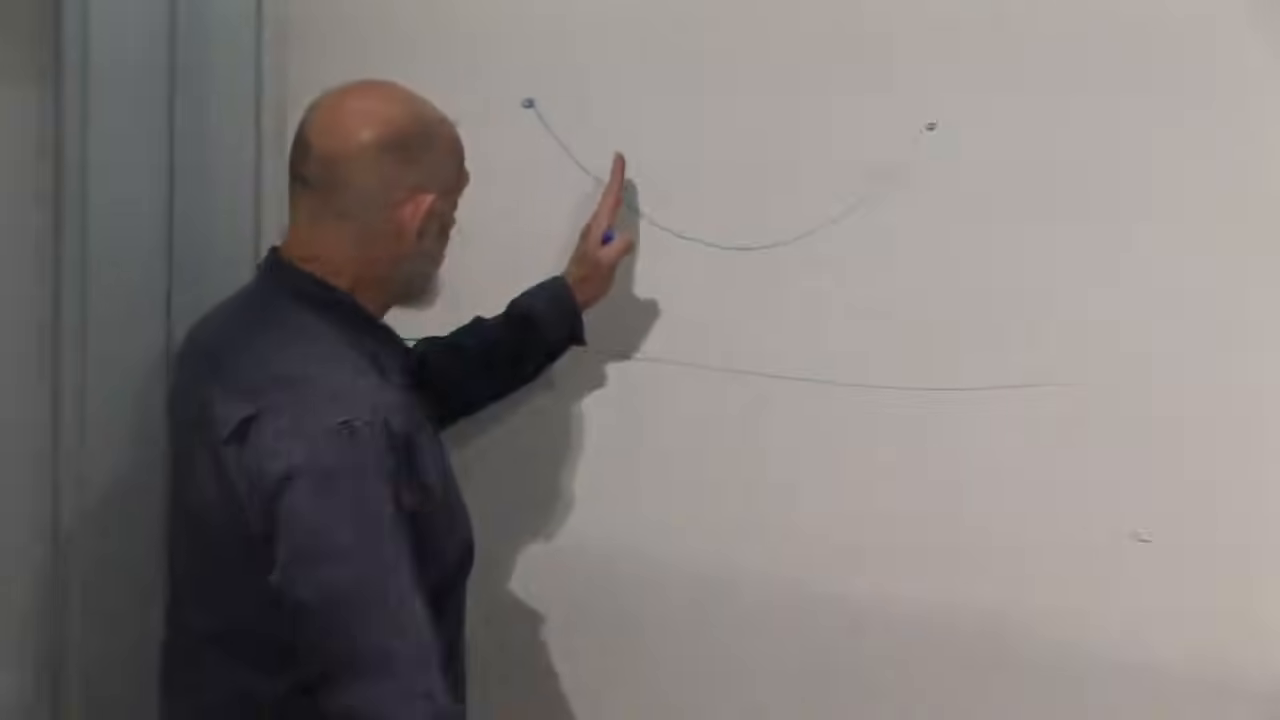
\includegraphics[width=0.76\textwidth]{lecture_03_figure_03.png}
  \caption{懸掛於固定支點之間的鏈條。其駐定形狀由總重力位能決定。}
  \lectureframe{00:30:41}
\end{figure}

這些例子有相同的架構：兩個固定端點、連接端點的函數，以及一個一階變分為零的積分。將這個整體條件化為微分方程，就是求解變分問題。

\section{力學中的邊界值問題}

畫軌跡時，通常把時間畫在水平軸上，因為\(t\)是自變數。不過，物理學中也有一個強烈的慣例：把時間畫成向上延伸。這裡插敘一則實驗：受試者依照與自身書寫系統相關的方向，排列從年輕到年老的人像；習慣由左至右閱讀的人多半由左至右排列，習慣由右至左閱讀的人則反向排列，而習慣縱向閱讀的人則縱向排列。笑話最後說，物理學家就是堅持時間向上流動的人。這裡仍採用慣例中的水平\(t\)軸，因為如此一來，\(x(t)\)自然可視為一張圖。

在初值問題中，\(t_0\)時刻給定的資料是
\begin{equation}
  x(t_0)=x_0,
  \qquad
  \dot x(t_0)=v_0.
  \label{eq:initial-value-data}
\end{equation}
牛頓方程接著決定此後的軌道。變分表述提出的是另一種問題：指定兩個端點事件，
\begin{equation}
  x(t_0)=x_0,
  \qquad
  x(t_1)=x_1,
  \label{eq:boundary-value-data}
\end{equation}
再求出兩事件之間的物理路徑。此時初速度不再是已知條件，而是解的一部分。

\begin{figure}[htbp]
  \centering
  \includegraphics[width=0.76\textwidth]{lecture_03_figure_09.png}
  \caption{一條力學軌跡\(x(t)\)。可以指定一端的位置與斜率，也可以指定兩個端點時刻的位置。}
  \lectureframe{00:27:41}
\end{figure}

要取駐值的量是\emph{作用量}：
\begin{equation}
  A[x]=\int_{t_0}^{t_1}L(x,\dot x,t)\,dt.
  \label{eq:action-one}
\end{equation}
被積函數\(L\)稱為\emph{拉格朗日量}，它可以依賴位置、速度，也可以顯式依賴時間。作用量原理寫作
\begin{equation}
  \delta A=0
  \label{eq:stationary-action}
\end{equation}
並要求路徑變分滿足
\begin{equation}
  \delta x(t_0)=\delta x(t_1)=0.
  \label{eq:fixed-endpoint-variations}
\end{equation}
端點條件至關重要：我們比較的是連接相同兩個事件的鄰近路徑。

\section{尤拉--拉格朗日方程的離散推導}

作用量是以無窮多個路徑上的函數值為輸入的泛函。為了具體計算它的變分，將時間區間切分成長度為\(\epsilon\)的小段，
\begin{equation}
  t_n=t_0+n\epsilon,
  \qquad
  x_n=x(t_n),
  \label{eq:discrete-times}
\end{equation}
並以以下差分近似第\(n\)個區間上的速度：
\begin{equation}
  v_n=\frac{x_{n+1}-x_n}{\epsilon}.
  \label{eq:discrete-velocity}
\end{equation}
於是，積分就成為一般的有限和：
\begin{equation}
  A_\epsilon
  =\sum_{n=0}^{N-1}
  \epsilon L\left(x_n,\frac{x_{n+1}-x_n}{\epsilon}\right).
  \label{eq:discrete-action}
\end{equation}
這裡用\(n\)表示時間切片的標號，讓\(i\)留待後文表示空間座標與粒子。

\begin{figure}[htbp]
  \centering
  \includegraphics[width=0.82\textwidth]{lecture_03_figure_10.png}
  \caption{將軌跡離散成一連串時間切片。改變一個內部點的高度，只會改變相鄰的兩個區段。}
  \lectureframe{00:38:30}
\end{figure}

改變一個內部點\(x_n\)，並保持其他所有\(x_k\)不變。總和中只有兩項依賴\(x_n\)：
\begin{align}
  A_\epsilon\big|_{x_n}
  &=
  \epsilon L\left(x_n,\frac{x_{n+1}-x_n}{\epsilon}\right)
  \notag\\
  &\quad+
  \epsilon L\left(x_{n-1},
                  \frac{x_n-x_{n-1}}{\epsilon}\right).
  \label{eq:two-neighbor-terms}
\end{align}
微分後得到
\begin{align}
  0=\frac{\partial A_\epsilon}{\partial x_n}
  &=
  \epsilon\frac{\partial L_n}{\partial x_n}
  -\frac{\partial L_n}{\partial v_n}
  +\frac{\partial L_{n-1}}{\partial v_{n-1}}.
  \label{eq:discrete-el-variation}
\end{align}
符號相反有簡單的幾何原因：提高\(x_n\)會增大它後方區間的斜率，並減小前方區間的斜率。

\begin{figure}[htbp]
  \centering
  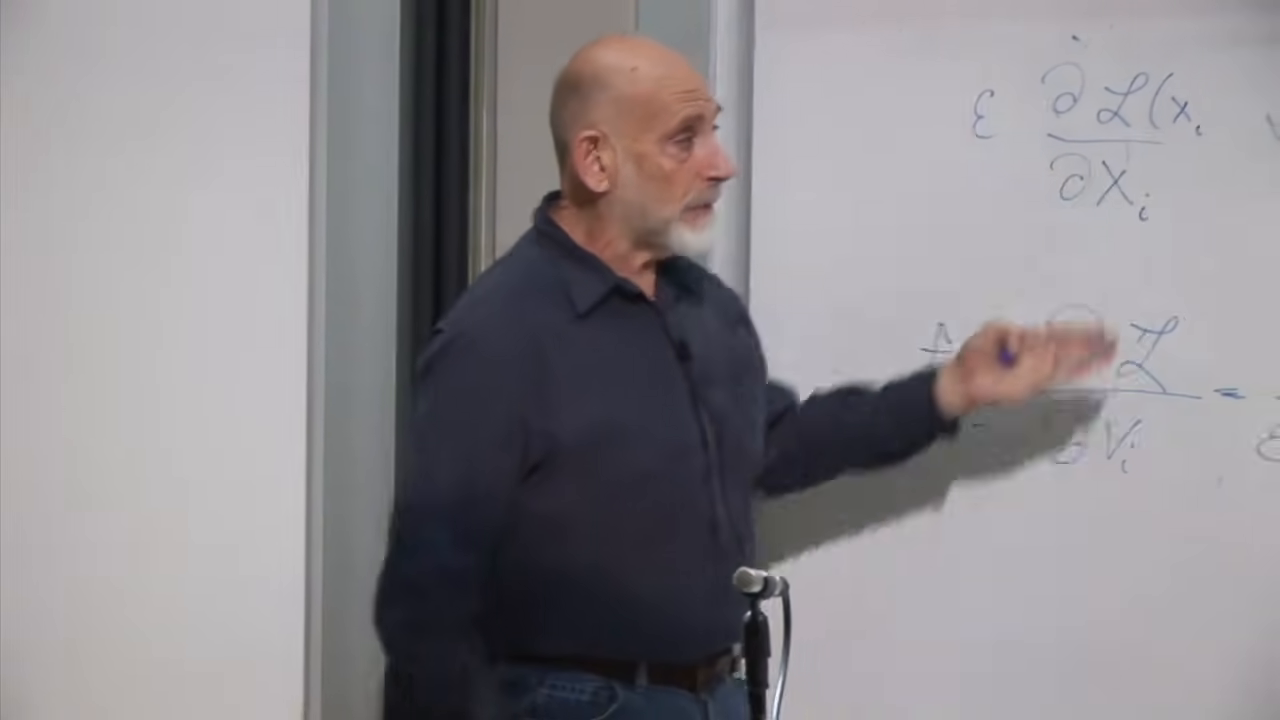
\includegraphics[width=0.74\textwidth]{lecture_03_figure_04.png}
  \caption{離散變分中的直接位置導數，以及兩個相鄰區間對速度導數的貢獻。}
  \lectureframe{00:45:26}
\end{figure}

將式~\eqref{eq:discrete-el-variation}重新整理：
\begin{equation}
  \frac{1}{\epsilon}
  \left(
    \frac{\partial L_n}{\partial v_n}
    -\frac{\partial L_{n-1}}{\partial v_{n-1}}
  \right)
  =
  \frac{\partial L_n}{\partial x_n}.
  \label{eq:discrete-el}
\end{equation}
左側是相鄰兩項的差商。當\(\epsilon\to0\)時，折線趨近光滑路徑，而差商也趨近時間導數：
\begin{equation}
  \boxed{
  \frac{d}{dt}\left(\frac{\partial L}{\partial\dot x}\right)
  =
  \frac{\partial L}{\partial x}}
  .
  \label{eq:euler-lagrange-one}
\end{equation}
這就是尤拉--拉格朗日方程。

\begin{figure}[htbp]
  \centering
  \includegraphics[width=0.78\textwidth]{lecture_03_figure_11.png}
  \caption{在每個內部時間切片都要求駐定後，得到完整的尤拉--拉格朗日方程。}
  \lectureframe{00:49:25}
\end{figure}

給定\(L\)之後，式~\eqref{eq:euler-lagrange-one}就像一部機器：對給定的函數做微分，便能得到路徑所滿足的微分方程。

\begin{classroomqa}
  \audiencequestion{尤拉--拉格朗日方程對任意的\(x\)與\(\dot x\)函數都成立嗎？\lecturetimestamp{00:49:37--00:50:24}}
  \lecturerresponse{是的，但函數必須具備進行所需微分的正則性。
  弧長的例子形式完全相同，只要把自變數\(x\)視為\(t\)，並把未知函數\(y(x)\)視為\(x(t)\)即可。這個例子的尤拉--拉格朗日方程以直線為解。}
\end{classroomqa}

\section{由拉格朗日量導出牛頓方程}

對於位於勢能\(V(x)\)中的直線運動粒子，取
\begin{equation}
  L(x,\dot x)=T-V
  =\frac12m\dot x^2-V(x).
  \label{eq:lagrangian-tv-one}
\end{equation}
負號看來或許奇怪，因為總能量是\(T+V\)。但拉格朗日量並不是能量。判斷它是否正確，要看尤拉--拉格朗日方程能否導出正確的運動。有人提議對正負號模擬投票，但這個提議被婉拒了：答案必須經過檢驗，不能靠投票決定。

首先，
\begin{equation}
  \frac{\partial L}{\partial\dot x}=m\dot x.
  \label{eq:conjugate-momentum-one}
\end{equation}
這就是動量。更一般地，與任意座標\(q\)共軛的動量定義為
\begin{equation}
  p_q=\frac{\partial L}{\partial\dot q}.
  \label{eq:conjugate-momentum-general}
\end{equation}
對式~\eqref{eq:conjugate-momentum-one}取時間導數，得到\(m\ddot x\)；另一方面，
\begin{equation}
  \frac{\partial L}{\partial x}
  =-\frac{dV}{dx}.
  \label{eq:lagrangian-position-derivative}
\end{equation}
因此尤拉--拉格朗日方程為
\begin{equation}
  m\ddot x=-\frac{dV}{dx}=F(x),
  \label{eq:newton-from-action}
\end{equation}
這就是牛頓第二定律。

\begin{figure}[htbp]
  \centering
  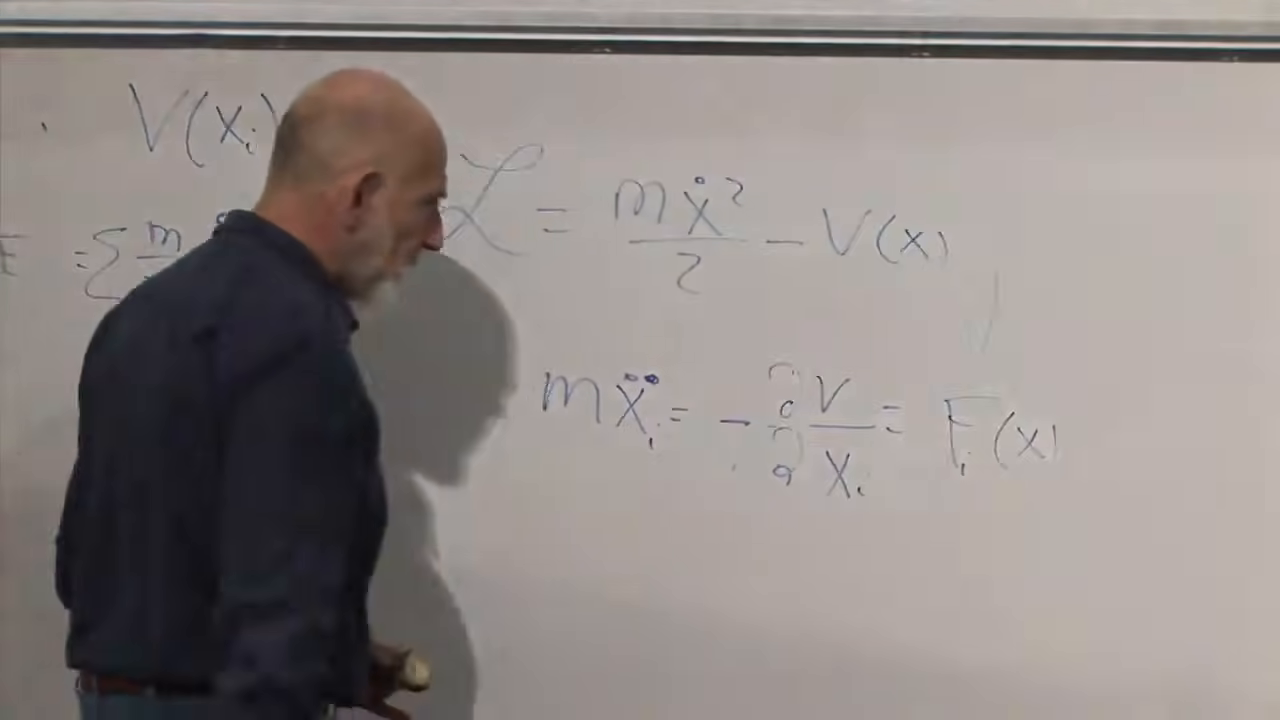
\includegraphics[width=0.80\textwidth]{lecture_03_figure_05.png}
  \caption{同一塊黑板上列出動能、位能、\(L=T-V\)，以及導出的牛頓方程分量形式。}
  \lectureframe{00:57:52}
\end{figure}

對多個座標\(q_i\)而言，
\begin{equation}
  L(\mathbf q,\dot{\mathbf q})
  =\sum_i\frac12m_i\dot q_i^{\,2}-V(q_1,q_2,\ldots),
  \label{eq:lagrangian-tv-many}
\end{equation}
每個座標都對應一個方程：
\begin{equation}
  \frac{d}{dt}\left(\frac{\partial L}{\partial\dot q_i}\right)
  =\frac{\partial L}{\partial q_i}
  \quad\Longrightarrow\quad
  m_i\ddot q_i=-\frac{\partial V}{\partial q_i}=F_i.
  \label{eq:euler-lagrange-many}
\end{equation}
軌跡仍是一條曲線，只是現在位於高維位形空間中。

\begin{classroomqa}
  \audiencequestion{我們是否只是從牛頓定律倒推，刻意構造出一個能重現結果的泛函？\lecturetimestamp{00:58:07--01:00:04}}
  \lecturerresponse{這不是最有成效的觀點。拉格朗日量是物理系統的精簡描述：一個包含所有座標與速度的函數，就能統整系統的所有運動方程。提出新理論時，物理學家通常先提出作用量，再由此推導方程，而不是逐一猜測每個方程。}
\end{classroomqa}

這種統整方式是一項優點，座標自由度則是另一項。直線最短，不會因為用笛卡兒座標、極座標或曲線座標描述平面而改變。同樣地，作用量取駐值的條件與座標系無關，儘管\(L\)的表達式和由此得到的分量方程會隨座標選擇而改變。

\section{從旋轉木馬上看自由粒子}

令\((x,y)\)為慣性笛卡兒座標，\((X,Y)\)為以角速度\(\omega\)均勻旋轉的座標。依照此處採用的方向約定，
\begin{align}
  x&=X\cos\omega t+Y\sin\omega t,
  \notag\\
  y&=-X\sin\omega t+Y\cos\omega t.
  \label{eq:rotating-coordinate-map}
\end{align}
兩座標系的夾角為\(\omega t\)。

\begin{figure}[htbp]
  \centering
  \includegraphics[width=0.76\textwidth]{lecture_03_figure_12.png}
  \caption{慣性笛卡兒座標軸與均勻旋轉的笛卡兒座標軸。同一個點在旋轉座標系中有隨時間變化的座標。}
  \lectureframe{01:06:05}
\end{figure}

自由粒子在慣性系中的拉格朗日量為
\begin{equation}
  L_{\mathrm{in}}
  =\frac{m}{2}\left(\dot x^2+\dot y^2\right).
  \label{eq:free-inertial-lagrangian}
\end{equation}
對式~\eqref{eq:rotating-coordinate-map}微分，並利用
\(\sin^2\omega t+\cos^2\omega t=1\)。三角函數項合併後可得
\begin{align}
  \dot x^2+\dot y^2
  &=
  \dot X^2+\dot Y^2\\
  &\quad+\omega^2(X^2+Y^2)\\
  &\quad+2\omega(Y\dot X-X\dot Y).
  \label{eq:rotating-speed}
\end{align}
因此
\begin{align}
  L_{\mathrm{rot}}
  &=
  \frac{m}{2}(\dot X^2+\dot Y^2)\\
  &\quad+\frac{m\omega^2}{2}(X^2+Y^2)\\
  &\quad+m\omega(Y\dot X-X\dot Y).
  \label{eq:rotating-lagrangian}
\end{align}

\begin{figure}[htbp]
  \centering
  \includegraphics[width=0.84\textwidth]{lecture_03_figure_13.png}
  \caption{變換後的自由粒子拉格朗日量：一般動能、一個二次離心項，以及一個對速度呈線性的項。}
  \lectureframe{01:12:16}
\end{figure}

二次座標項的形式為\(-V_{\mathrm{fict}}\)，其中
\begin{equation}
  V_{\mathrm{fict}}
  =-\frac{m\omega^2}{2}(X^2+Y^2).
  \label{eq:centrifugal-potential}
\end{equation}
此項隨著距離旋轉軸愈遠而減小，因此產生離心力
\(m\omega^2(X,Y)\)。

式~\eqref{eq:rotating-lagrangian}的最後一項對座標與速度都是線性的。套用尤拉--拉格朗日方程可得
\begin{align}
  m\ddot X&=m\omega^2X-2m\omega\dot Y,
  \notag\\
  m\ddot Y&=m\omega^2Y+2m\omega\dot X.
  \label{eq:rotating-equations}
\end{align}
與\(\omega^2\)成正比的項是離心項，與速度成正比的項則是科里奧利項。在旋轉平面內，向量形式為
\begin{equation}
  \mathbf F_{\mathrm{C}}
  =-2m\,\boldsymbol\omega\times\mathbf v_{\mathrm{rot}},
  \label{eq:coriolis-vector}
\end{equation}
若採用相反的方向約定，符號也會相應改變。

\begin{figure}[htbp]
  \centering
  \includegraphics[width=0.84\textwidth]{lecture_03_figure_14.png}
  \caption{旋轉座標系中的方程：與座標成正比的項給出離心加速度，與交叉速度成正比的項則給出科里奧利加速度。}
  \lectureframe{01:20:20}
\end{figure}

重點不在於代數運算消失了，而在於對一個純量函數做一次座標變換，就能同時導出兩個耦合方程與兩種慣性力。

\begin{classroomqa}
  \audiencequestion{這個方法也適用於任意曲線座標嗎？\lecturetimestamp{01:22:01--01:22:17}}
  \lecturerresponse{適用。新座標可以是曲線座標，也可以像旋轉座標一樣顯式依賴時間。只要用新變數改寫作用量，再套用相同的尤拉--拉格朗日法則即可。}
\end{classroomqa}

\section{極座標與循環座標}

在一般極座標中，
\begin{equation}
  x=r\cos\theta,
  \qquad
  y=r\sin\theta.
  \label{eq:polar-map}
\end{equation}
\(r\)和\(\theta\)都可以隨時間變化。對座標取時間導數，再將平方項相加，可得
\begin{equation}
  \dot x^2+\dot y^2
  =\dot r^2+r^2\dot\theta^2.
  \label{eq:polar-speed}
\end{equation}
若中心勢能為\(V(r)\)，則
\begin{equation}
  L
  =\frac{m}{2}\left(\dot r^2+r^2\dot\theta^2\right)-V(r).
  \label{eq:polar-lagrangian}
\end{equation}

\begin{figure}[htbp]
  \centering
  \includegraphics[width=0.80\textwidth]{lecture_03_figure_15.png}
  \caption{極座標幾何，以及動能在徑向運動與角向運動間的分解。}
  \lectureframe{01:23:30}
\end{figure}

徑向方程為
\begin{equation}
  m\ddot r
  =mr\dot\theta^2-\frac{dV}{dr}.
  \label{eq:radial-equation}
\end{equation}
第一項是由粒子自身的角向運動所造成的向外離心效應。

對角座標而言，
\begin{equation}
  \frac{d}{dt}\left(\frac{\partial L}{\partial\dot\theta}\right)
  =\frac{\partial L}{\partial\theta}=0,
  \label{eq:theta-el}
\end{equation}
因為中心勢能沒有顯式的\(\theta\)依賴性。因此
\begin{equation}
  \frac{d}{dt}\left(mr^2\dot\theta\right)=0,
  \qquad
  mr^2\dot\theta=\ell,
  \label{eq:angular-momentum}
\end{equation}
其中\(\ell\)是守恆的角動量。

\begin{figure}[htbp]
  \centering
  \includegraphics[width=0.82\textwidth]{lecture_03_figure_16.png}
  \caption{角座標的尤拉--拉格朗日方程右側為零，因此顯示出\(mr^2\dot\theta\)守恆。}
  \lectureframe{01:29:25}
\end{figure}

角向方程給出
\begin{equation}
  \dot\theta=\frac{\ell}{mr^2}.
  \label{eq:theta-dot-angular-momentum}
\end{equation}
將此結果代入式~\eqref{eq:radial-equation}，便得到只含\(r\)的一個方程：
\begin{equation}
  m\ddot r
  =\frac{\ell^2}{mr^3}-\frac{dV}{dr}.
  \label{eq:effective-radial-equation}
\end{equation}

不出現在\(L\)中的座標，傳統上稱為\emph{循環}座標，即使它不是角度也一樣。若\(q\)是循環座標，則
\begin{equation}
  \frac{\partial L}{\partial q}=0
  \quad\Longrightarrow\quad
  \frac{d}{dt}\left(\frac{\partial L}{\partial\dot q}\right)=0.
  \label{eq:cyclic-conservation}
\end{equation}
其共軛動量便是守恆量。這初步揭示了對稱性與守恆定律之間的一般關係。

\section{關於意義、能量與適用範圍的問題}

接下來的問題將點出這套形式體系更深層的內涵。

\begin{classroomqa}
  \audiencequestion{除了發現拉格朗日量能導出正確的經典方程之外，還有其他獨立的理由可以得到拉格朗日量嗎？\lecturetimestamp{01:33:25--01:35:07}}
  \lecturerresponse{從歷史上看，經典力學在一個多世紀的發展中，已證明粒子、波與電磁場都能寫成這種形式。在經典層次上，這些累積的成功，是關於自然定律如何組織起來的經驗事實。更深層的解釋來自量子力學，這裡暫且不談。}
\end{classroomqa}

\begin{classroomqa}
  \audiencequestion{旋轉座標系中的拉格朗日量裡，對速度呈線性的項能否視為一般的動能或位能？\lecturetimestamp{01:35:08--01:36:23}}
  \lecturerresponse{不能。與時間平移對稱性相關的守恆量，是由哈密頓量的構造方式導出的，不能把\(L\)中的每一項都直接解讀為動能或位能。對式~\eqref{eq:rotating-lagrangian}而言，對速度呈線性的項在\(\sum_a\dot q_a\,\partial L/\partial\dot q_a-L\)中會相消。哈密頓形式將有系統地整理這個問題。}
\end{classroomqa}

確實，由於\(L_{\mathrm{rot}}\)沒有顯式的時間依賴性，
\begin{equation}
  \begin{aligned}
    H_{\mathrm{rot}}
    &=\dot X\frac{\partial L}{\partial\dot X}
     +\dot Y\frac{\partial L}{\partial\dot Y}-L\\
    &=\frac{m}{2}(\dot X^2+\dot Y^2)
     -\frac{m\omega^2}{2}(X^2+Y^2)
  \end{aligned}
  \label{eq:rotating-hamiltonian-preview}
\end{equation}
是守恆量。它是旋轉座標系中的雅可比積分，數值上並不等同於慣性觀察者所賦予的能量。依賴時間的座標變換不一定保留能量的數值形式。

\begin{classroomqa}
  \audiencequestion{如果曲線軌跡是由重力造成的呢？\lecturetimestamp{01:36:30--01:37:10}}
  \lecturerresponse{對於牛頓重力，只要在中心力拉格朗日量中取\(V(r)=-GMm/r\)即可。彎曲時空屬於廣義相對論，這裡不予採用。}
\end{classroomqa}

\begin{classroomqa}
  \audiencequestion{離心位能及其能量只是虛構的嗎？\lecturetimestamp{01:37:13--01:40:14}}
  \lecturerresponse{旋轉平台上的觀察者可以測量有效力，也能一致地使用旋轉座標系中的守恆量。\emph{虛構}表示這些項源自非慣性座標系的描述，並不表示它們造成的可觀測效應是假的。一般而言，能量在依賴時間的座標變換下並非不變。}
\end{classroomqa}

\begin{classroomqa}
  \audiencequestion{與速度相關的科里奧利力指向哪個方向？\lecturetimestamp{01:40:22--01:42:36}}
  \lecturerresponse{它垂直於旋轉座標系中的速度，大小與速率和座標系的角速度成正比。在平面內，兩個分量會分別交換\(\dot X\)與\(\dot Y\)，並帶有相反的符號，如式~\eqref{eq:rotating-equations}所示。}
\end{classroomqa}

\begin{figure}[htbp]
  \centering
  \includegraphics[width=0.76\textwidth]{lecture_03_figure_17.png}
  \caption{交叉速度分量的形式：科里奧利力垂直於旋轉座標系中的速度。}
  \lectureframe{01:41:40}
\end{figure}

\begin{classroomqa}
  \audiencequestion{起始拉格朗日量一定要在慣性系中寫出嗎？\lecturetimestamp{01:42:37--01:44:00}}
  \lecturerresponse{對一般的自由粒子而言，牛頓的慣性系定律提供了簡單的起始形式\(m(\dot x^2+\dot y^2)/2\)。知道這條物理定律後，就可以將作用量轉換到其他任何座標系。不應另外假設旋轉座標系中也有相同的簡單動能公式。}
\end{classroomqa}

磁場中的帶電粒子也會出現同類的速度線性項：
\begin{equation}
  L_{\mathrm{em}}
  =\frac12m\mathbf v^2
   +q\mathbf A(\mathbf r,t)\cdot\mathbf v
   -q\phi(\mathbf r,t).
  \label{eq:electromagnetic-lagrangian}
\end{equation}
若均勻磁場垂直於平面，採用對稱規範\(\mathbf A=\tfrac12\mathbf B\times\mathbf r\)便會產生一個與\(X\dot Y-Y\dot X\)成正比的項，其代數形式與科里奧利項相同。

\begin{figure}[htbp]
  \centering
  \includegraphics[width=0.82\textwidth]{lecture_03_figure_18.png}
  \caption{旋轉座標系中的速度線性項，讓我們得以將它與均勻磁場中的帶電粒子作比較。}
  \lectureframe{01:44:40}
\end{figure}

\begin{classroomqa}
  \audiencequestion{除了光滑性之外，作為拉格朗日量的函數還必須符合哪些條件？\lecturetimestamp{01:44:46--01:45:06}}
  \lecturerresponse{有，但相關限制需要更多尚未介紹的數學架構，因此留待後續討論。現階段的核心要點是：提出一個拉格朗日量，就能由它導出方程與守恆定律。}
\end{classroomqa}

旋轉系方程也允許圓周運動：在慣性系中靜止的點，從旋轉木馬上看會繞著旋轉原點轉動。磁場的類比則說明了帶電粒子為何能作迴旋運動。

\begin{classroomqa}
  \audiencequestion{帶電粒子會一直沿著那個圓運動，還是會因輻射而使軌道塌縮？\lecturetimestamp{01:46:11--01:47:21}}
  \lecturerresponse{目前討論的粒子方程沒有納入輻射。若將粒子與電磁場的耦合以及輻射反作用一併納入，加速的經典電荷便會輻射。因此，輻射是額外的物理效應，並不與簡化方程中的軌道相矛盾。}
\end{classroomqa}

\begin{classroomqa}
  \audiencequestion{颶風與這個討論有什麼關係？
  \lecturetimestamp{01:47:30--01:47:50}}
  \lecturerresponse{颶風的大尺度大氣運動發生在旋轉的地球上，因此科里奧利效應很重要。完整的推導屬於氣象學範疇，這裡不會展開。}
\end{classroomqa}

\begin{classroomqa}
  \audiencequestion{作用量架構預期能涵蓋每一條物理定律嗎？若真有例外，又代表什麼？\lecturetimestamp{01:47:57--01:49:01}}
  \lecturerresponse{在此處討論範圍內，所有已知的封閉基礎理論都能用作用量來組織，包括牛頓粒子、麥克斯威場、廣義相對論與標準模型。黏滯阻力等表面上的反例，是因為省略了環境自由度才出現。若把流體或微觀熱浴也納入系統，基礎描述仍符合這套架構。因此，若發現真正基礎的例外，將會是重大發現。}
\end{classroomqa}
\chapter{對稱性與守恆定律}

\lectureoverview{駐值作用量原理與尤拉--拉格朗日方程構成經典力學核心的一半；另一半則是哈密頓表述。本節將充分發展前半部分，揭示一個深刻的規律：拉格朗日量的每個連續對稱性都會產生一個守恆量。我們將從平移和旋轉中找出這個規律，證明它適用於一般的無窮小變換，接著仔細考察這項論證在哪些情況下適用、哪些情況下不適用。}

\section{解釋物理所需的最低限度數學}

黑板上已有的符號看起來或許有點像薛丁格方程，但今晚的主題不是它。主題是對稱性與守恆。若不使用方程，就無法如實解釋兩者的關聯。這些方程很初等；關鍵在於如何安排它們，讓背後的結構顯現出來。《科學美國人》或許會為這個結果命名，但在這裡，我們要的是物理學家推導它所需的最低限度數學。

引入一個小參數\(\epsilon\)。我們保留正比於\(\epsilon\)的項，捨去\(O(\epsilon^2)\)。這只是極限論證的簡寫，並不是說非零實數的平方真的等於零。對一般函數\(f(x,y)\)，
\begin{equation}
  \delta f
  =\frac{\partial f}{\partial x}\,\delta x
   +\frac{\partial f}{\partial y}\,\delta y
   +O(\epsilon^2),
  \label{eq:first-variation-f}
\end{equation}
其中\(\delta x\)和\(\delta y\)都正比於\(\epsilon\)。符號\(\delta f\)表示\(f\)的變化，不是把稱為\(\delta\)的數乘上\(f\)。駐點滿足
\begin{equation}
  \delta f=0
  \qquad\hbox{to first order.}
  \label{eq:stationary-f}
\end{equation}

對力學路徑\(q_i(t)\)而言，相應的量是作用量
\begin{equation}
  S[q]=\int_{t_1}^{t_2}L(q,\dot q,t)\,dt.
  \label{eq:action-l4}
\end{equation}
固定路徑端點後對路徑作變分，得到
\begin{equation}
  \delta S
  =\int_{t_1}^{t_2}dt\,
   \sum_i\left(
     \frac{\partial L}{\partial q_i}\,\delta q_i
     +\frac{\partial L}{\partial\dot q_i}\,\delta\dot q_i
   \right).
  \label{eq:action-variation-l4}
\end{equation}
這兩項之所以出現，是因為改變路徑會同時改變位置和速度。利用分部積分以及
\(\delta q_i(t_1)=\delta q_i(t_2)=0\)，可將\(\delta S=0\)化為
\begin{equation}
  \frac{d}{dt}\left(\frac{\partial L}{\partial\dot q_i}\right)
  -\frac{\partial L}{\partial q_i}=0.
  \label{eq:el-l4}
\end{equation}

\begin{figure}[htbp]
  \centering
  \includegraphics[width=0.76\textwidth]{lecture_04_figure_05.png}
  \caption{回顧尤拉--拉格朗日方程，作為討論對稱性與守恆的出發點。}
  \lectureframe{00:09:00}
\end{figure}

正確的說法是\emph{作用量駐值}，不一定是作用量最小。這項區別將在接近結尾時再次提到。

\section{廣義座標與共軛動量}

笛卡兒位置不足以描述一般力學。座標可以是粒子的位置、角度、集體變數或場振幅，因此我們稱它們為\(q_i\)。拉格朗日量是對動力學的精簡描述。即使是標準模型，若不用高度濃縮的記號寫出來，也大約占一頁；若為每個場分量分別寫出運動方程，篇幅會大得多。一個函數\(L\)就將這些內容全部囊括其中。

與\(q_i\)共軛的動量為
\begin{equation}
  p_i=\frac{\partial L}{\partial\dot q_i}.
  \label{eq:canonical-momentum-l4}
\end{equation}
因此，廣義座標傳統上以\(q\)表示，相應的動量則以\(p\)表示，形成\(p\)和\(q\)這套記號。在這套記號下，式~\eqref{eq:el-l4}變為
\begin{equation}
  \dot p_i=\frac{\partial L}{\partial q_i}.
  \label{eq:momentum-el-l4}
\end{equation}

對熟悉的一維粒子而言，
\begin{equation}
  L=\frac{m\dot x^2}{2}-V(x),
  \qquad
  \frac{\partial L}{\partial\dot x}=m\dot x,
  \label{eq:particle-momentum-l4}
\end{equation}
因此，共軛動量就是通常的動量。

\begin{figure}[htbp]
  \centering
  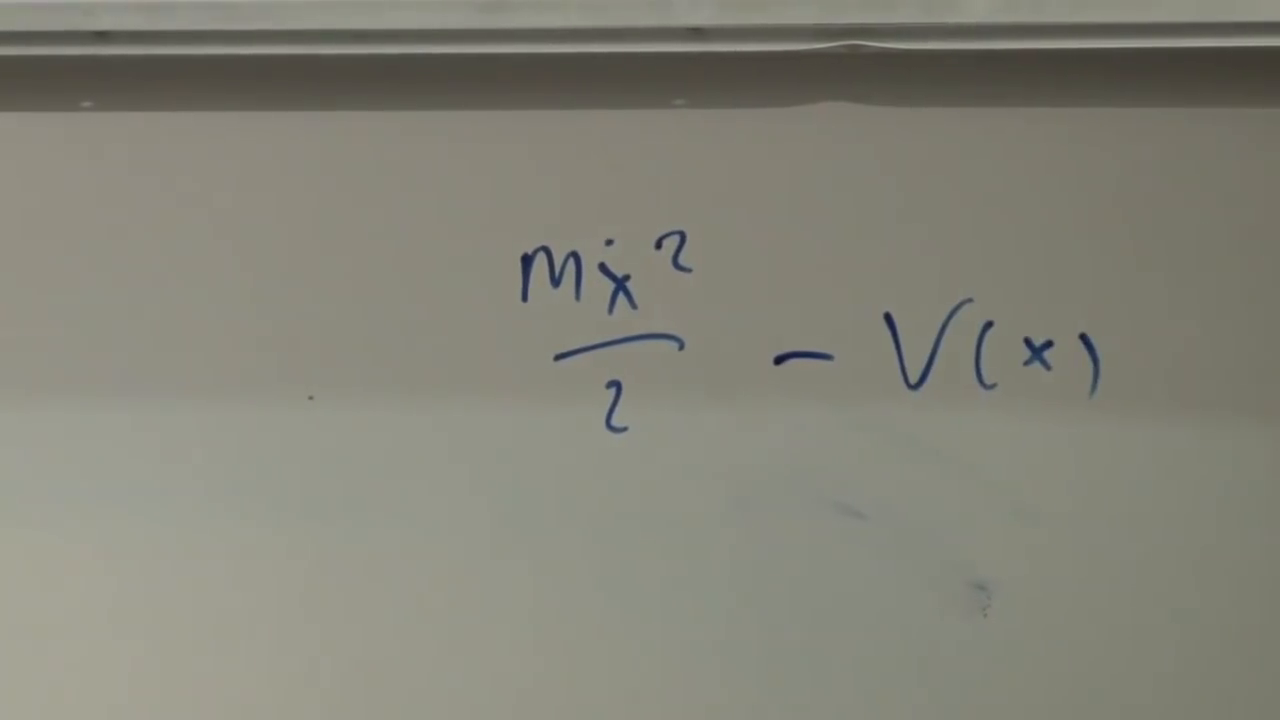
\includegraphics[width=0.72\textwidth]{lecture_04_figure_02.png}
  \caption{以動能減勢能的拉格朗日量說明共軛動量為\(m\dot x\)。}
  \lectureframe{00:14:48}
\end{figure}

如果\(q_i\)沒有出現在\(L\)中，那麼\(\dot p_i=0\)。這是利用循環座標導出守恆律的常見方法。兩者之間的真正關聯更為一般；先從例子中找出這種關聯，再加以證明，會更有幫助。

\section{尚未解釋便先找到的守恆定律}

\subsection{兩個座標與依賴間距的勢能}

令兩個質量都等於一，並取
\begin{equation}
  L=\frac{\dot q_1^{\,2}+\dot q_2^{\,2}}{2}-V(q_1-q_2).
  \label{eq:separation-lagrangian}
\end{equation}
可以想像兩個粒子在一條直線上運動。它們的交互作用只依賴彼此的間距。

\begin{figure}[htbp]
  \centering
  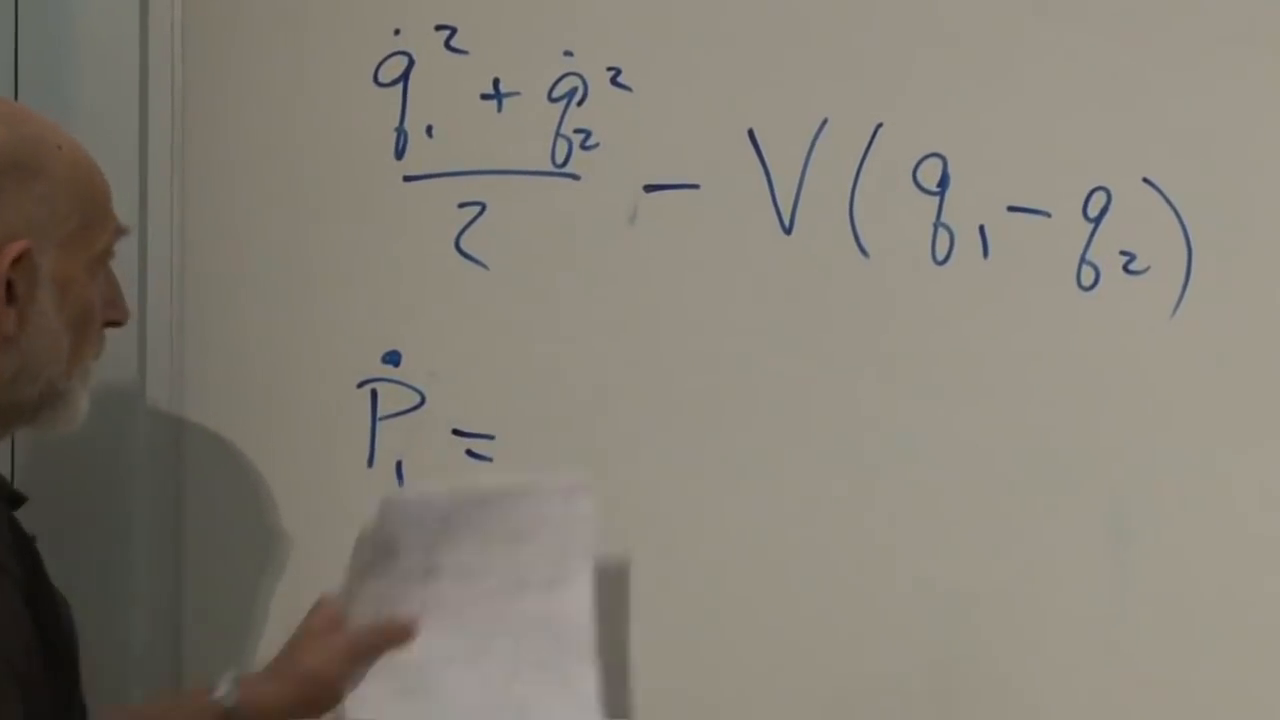
\includegraphics[width=0.78\textwidth]{lecture_04_figure_03.png}
  \caption{雙座標拉格朗日量，以及第一個動量方程的推導起點。}
  \lectureframe{00:18:56}
\end{figure}

以\(V'\)表示對\(V\)的自變數求導，
\begin{align}
  \dot p_1&=-V'(q_1-q_2),
  \notag\\
  \dot p_2&=+V'(q_1-q_2).
  \label{eq:separation-momentum-equations}
\end{align}
第二個方程的符號相反，因為增加\(q_2\)會使\(q_1-q_2\)減小。

\begin{classroomqa}
  \audiencequestion{第一個動量方程是否應該包含\(V'\)？負號從何而來？
  \lecturetimestamp{00:20:52--00:21:35}}
  \lecturerresponse{尤拉--拉格朗日方程表示
  \(\dot p_1=\partial L/\partial q_1\)，並不是說拉格朗日量等於零。由於\(L=T-V\)，對\(q_1\)微分會得到
  \(-V'\)。對\(q_2\)微分時，又因為\(q_1-q_2\)而多出一個負號，所以第二個方程中會出現\(+V'\)。}
\end{classroomqa}

\begin{figure}[htbp]
  \centering
  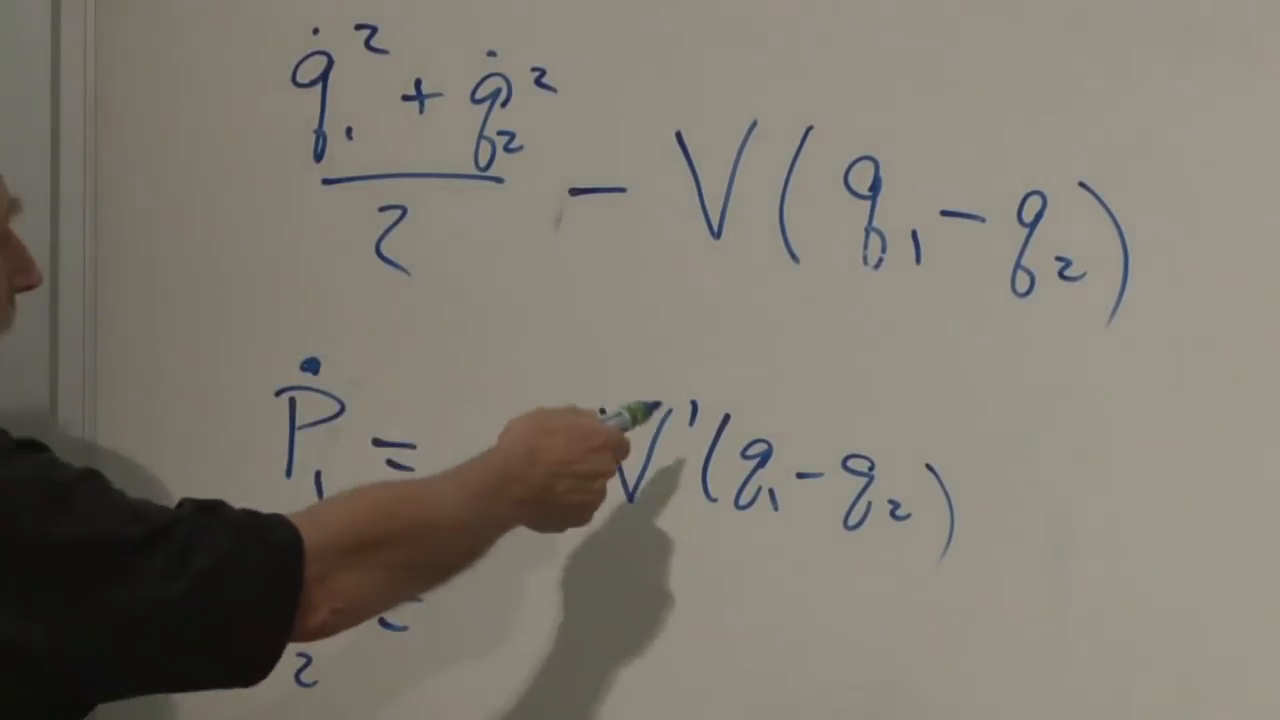
\includegraphics[width=0.78\textwidth]{lecture_04_figure_04.png}
  \caption{對\(p_1\)方程而言，導數的符號至關重要；\(p_2\)方程則有相反的符號。}
  \lectureframe{00:20:41}
\end{figure}

將式~\eqref{eq:separation-momentum-equations}相加，得到
\begin{equation}
  \frac{d}{dt}(p_1+p_2)=0.
  \label{eq:total-p-conserved}
\end{equation}
我們找到了守恆量，但還沒有解釋它為何存在。

\subsection{一個較不明顯的線性組合}

現在令
\begin{equation}
  L=\frac{\dot q_1^{\,2}+\dot q_2^{\,2}}{2}
    -V(Aq_1+Bq_2),
  \label{eq:ab-lagrangian}
\end{equation}
其中\(A\)和\(B\)是常數。於是
\begin{align}
  \dot p_1&=-A\,V'(Aq_1+Bq_2),
  \notag\\
  \dot p_2&=-B\,V'(Aq_1+Bq_2).
  \label{eq:ab-momentum-equations}
\end{align}
將第一個方程乘以\(B\)，第二個方程乘以\(A\)，再相減，就能消去力項：
\begin{equation}
  \frac{d}{dt}(Bp_1-Ap_2)=0.
  \label{eq:ab-conserved}
\end{equation}

\begin{figure}[htbp]
  \centering
  \includegraphics[width=0.78\textwidth]{lecture_04_figure_06.png}
  \caption{加權後的動量方程；力項在\(Bp_1-Ap_2\)中相消。}
  \lectureframe{00:24:20}
\end{figure}

\begin{classroomqa}
  \audiencequestion{從物理角度來看，像\(A\)和\(B\)這樣的常數可能從何而來？\lecturetimestamp{00:25:09--00:30:15}}
  \lecturerresponse{考慮兩個質量分別為\(m\)和\(M\)的粒子：
  \[
    L=\frac{m\dot X^2}{2}+\frac{M\dot Y^2}{2}-V(X-Y).
  \]
  重新定義尺度，使\(Q_1=\sqrt m\,X\)和\(Q_2=\sqrt M\,Y\)成立。動能項
  變為\((\dot Q_1^2+\dot Q_2^2)/2\)，而勢能則依賴於
  \(Q_1/\sqrt m-Q_2/\sqrt M\)。因此，不同的質量自然會成為線性組合中的係數。將\(Q_2\)換成\(-Q_2\)，會讓寫出的減號變成加號，而平方後的動能項不變。}
\end{classroomqa}

\begin{figure}[htbp]
  \centering
  \includegraphics[width=0.82\textwidth]{lecture_04_figure_07.png}
  \caption{質量加權座標使動能項更簡潔，同時將質量因子移入勢能。}
  \lectureframe{00:28:40}
\end{figure}

\begin{classroomqa}
  \audiencequestion{這是否表示，即使沒有循環座標，也可能存在守恆量？\lecturetimestamp{00:31:13--00:31:58}}
  \lecturerresponse{按目前寫出的變數來看，沒有\emph{明顯的}循環座標。變數變換或許能找出一個循環座標，但在這裡，尋找循環座標並不是有用的切入點。對稱性論證會直接找出守恆的組合。}
\end{classroomqa}

\section{對稱性的意義}

\subsection{平移}

先考慮質量為一的自由粒子，
\begin{equation}
  L=\frac{\dot q^2}{2}.
  \label{eq:free-unit-l4}
\end{equation}
將其運動歷程中的每一點都平移相同的常數：
\begin{equation}
  q'(t)=q(t)+\epsilon.
  \label{eq:free-translation}
\end{equation}
由於\(\epsilon\)與時間無關，\(\dot q'=\dot q\)，因此
\(\delta L=0\)。這種不變性就是平移對稱性。

有兩種等價的觀點。被動觀點是移動座標原點、物體則保持不動；主動觀點是固定座標軸、移動物體。採用主動的說法較不容易混淆：移動物理構型，看看\(L\)是否察覺。

對式~\eqref{eq:separation-lagrangian}而言，將兩個座標都平移：
\begin{equation}
  \delta q_1=\epsilon,
  \qquad
  \delta q_2=\epsilon.
  \label{eq:common-translation}
\end{equation}
速度不變，\(q_1-q_2\)也不變。

\begin{figure}[htbp]
  \centering
  \includegraphics[width=0.78\textwidth]{lecture_04_figure_08.png}
  \caption{共同平移不會改變兩個座標之間的距離。}
  \lectureframe{00:35:30}
\end{figure}

對式~\eqref{eq:ab-lagrangian}而言，採用較不明顯的變換
\begin{equation}
  \delta q_1=B\epsilon,
  \qquad
  \delta q_2=-A\epsilon.
  \label{eq:ab-transformation}
\end{equation}
速度同樣不變，而且
\begin{equation}
  \delta(Aq_1+Bq_2)=AB\epsilon-BA\epsilon=0.
  \label{eq:ab-invariant-argument}
\end{equation}
因此，這個變換是一種對稱性。

\begin{figure}[htbp]
  \centering
  \includegraphics[width=0.80\textwidth]{lecture_04_figure_09.png}
  \caption{保持\(Aq_1+Bq_2\)不變的非對稱平移。}
  \lectureframe{00:40:20}
\end{figure}

\begin{classroomqa}
  \audiencequestion{這些係數是否代表質量，使守恆量成為通常所說的質心動量？
  \lecturetimestamp{00:42:25--00:42:45}}
  \lecturerresponse{是。在質量加權變數中，對稱性和守恆量的組合看起來不對稱。換回\(X\)和\(Y\)後，就會得到通常的整體平移和總動量。}
\end{classroomqa}

\subsection{旋轉}

考慮平面中的單一粒子，
\begin{equation}
  L=\frac{m}{2}(\dot x^2+\dot y^2)-V(x^2+y^2).
  \label{eq:central-lagrangian-l4}
\end{equation}
這是中心力場的勢能。我們比較兩個彼此相對旋轉但各自固定的座標系；座標軸不會隨時間轉動。採用一致的旋轉方向，
\begin{align}
  x'&=x\cos\theta+y\sin\theta,
  \notag\\
  y'&=-x\sin\theta+y\cos\theta.
  \label{eq:finite-rotation-l4}
\end{align}

\begin{figure}[htbp]
  \centering
  \includegraphics[width=0.82\textwidth]{lecture_04_figure_10.png}
  \caption{中心力場的拉格朗日量，以及兩個經旋轉彼此對應的固定笛卡兒座標系。}
  \lectureframe{00:45:40}
\end{figure}

令\(\theta=\epsilon\)，並保留一階項：
\begin{equation}
  \cos\epsilon=1+O(\epsilon^2),
  \qquad
  \sin\epsilon=\epsilon+O(\epsilon^3).
  \label{eq:small-angle-l4}
\end{equation}
無窮小旋轉為
\begin{align}
  \delta x&=y\epsilon,
  &\delta y&=-x\epsilon,
  \notag\\
  \delta\dot x&=\dot y\epsilon,
  &\delta\dot y&=-\dot x\epsilon.
  \label{eq:infinitesimal-rotation-l4}
\end{align}

\begin{figure}[htbp]
  \centering
  \includegraphics[width=0.82\textwidth]{lecture_04_figure_11.png}
  \caption{座標和速度的無窮小旋轉。}
  \lectureframe{00:49:50}
\end{figure}

平移時，座標的改變量與原座標無關；旋轉則不同，\(x\)的改變量取決於\(y\)，而\(y\)的改變量取決於\(x\)。儘管如此，
\begin{align}
  \delta(x^2+y^2)
  &=2x\,\delta x+2y\,\delta y=0,
  \notag\\
  \delta(\dot x^2+\dot y^2)
  &=2\dot x\,\delta\dot x+2\dot y\,\delta\dot y=0.
  \label{eq:rotation-invariants-l4}
\end{align}
勢能項和動能項都保持不變。

\begin{figure}[htbp]
  \centering
  \includegraphics[width=0.76\textwidth]{lecture_04_figure_12.png}
  \caption{一階項相消，證明半徑平方在旋轉下不變。}
  \lectureframe{00:53:20}
\end{figure}

\section{一般守恆定理}

平移和旋轉這兩個例子有共同的形式。令一個連續的無窮小變換為
\begin{equation}
  \delta q_i=\epsilon f_i(q),
  \qquad
  \delta\dot q_i=\frac{d}{dt}\delta q_i,
  \label{eq:general-infinitesimal-symmetry}
\end{equation}
其中\(\epsilon\)與時間無關，而\(f_i\)可以依賴所有座標。

\begin{figure}[htbp]
  \centering
  \includegraphics[width=0.78\textwidth]{lecture_04_figure_13.png}
  \caption{一般的無窮小位移場
  \(\delta q_i=\epsilon f_i(q)\)。}
  \lectureframe{00:56:00}
\end{figure}

拉格朗日量的一階變分為
\begin{equation}
  \delta L
  =\sum_i\left(
    \frac{\partial L}{\partial q_i}\delta q_i
    +\frac{\partial L}{\partial\dot q_i}\delta\dot q_i
  \right).
  \label{eq:delta-l-general}
\end{equation}

\begin{figure}[htbp]
  \centering
  \includegraphics[width=0.84\textwidth]{lecture_04_figure_14.png}
  \caption{對\(\delta L\)的兩項貢獻：座標變分與速度變分。}
  \lectureframe{01:02:30}
\end{figure}

現在只考慮物理路徑，亦即尤拉--拉格朗日方程成立的路徑。利用
\begin{equation}
  \frac{\partial L}{\partial\dot q_i}=p_i,
  \qquad
  \frac{\partial L}{\partial q_i}=\dot p_i,
  \label{eq:el-substitution-l4}
\end{equation}
可得
\begin{align}
  \delta L
  &=\sum_i\left(\dot p_i\,\delta q_i
                +p_i\,\delta\dot q_i\right)
  \notag\\
  &=\frac{d}{dt}\sum_i p_i\delta q_i
  =\epsilon\frac{d}{dt}\sum_i p_i f_i(q).
  \label{eq:noether-derivation-l4}
\end{align}
關鍵步驟只用到乘法法則。

若此變換是對稱性，則\(\delta L=0\)。由於\(\epsilon\)是任意常數因子，
\begin{equation}
  \boxed{
  \frac{d\mathcal Q}{dt}=0,
  \qquad
  \mathcal Q=\sum_i p_i f_i(q)}
  .
  \label{eq:noether-charge-l4}
\end{equation}
這就是諾特定理在經典力學中的核心，適用於精確且不含時的點對稱性。

\begin{figure}[htbp]
  \centering
  \includegraphics[width=0.84\textwidth]{lecture_04_figure_15.png}
  \caption{利用乘法法則，從\(L\)的不變性導出守恆量。}
  \lectureframe{01:05:00}
\end{figure}

\begin{classroomqa}
  \audiencequestion{在\(f_i(q)\)中，\(q\)是否還有另一個指標？
  \lecturetimestamp{01:06:57--01:07:31}}
  \lecturerresponse{沒有指標的\(q\)代表整個集合\((q_1,q_2,\ldots)\)。每個分量\(f_i\)都可以依賴這些座標中的所有座標。例如，旋轉時\(f_x=y\)且\(f_y=-x\)。}
\end{classroomqa}

現在可以看出，這些例子並非偶然。共同平移有\(f_1=f_2=1\)，因此
\begin{equation}
  \mathcal Q=p_1+p_2.
  \label{eq:noether-common-p}
\end{equation}
非對稱平移有\(f_1=B\)和\(f_2=-A\)，因此
\begin{equation}
  \mathcal Q=Bp_1-Ap_2.
  \label{eq:noether-ab-p}
\end{equation}
旋轉時，\(f_x=y\)且\(f_y=-x\)：
\begin{equation}
  \mathcal Q=p_xy-p_yx.
  \label{eq:rotation-charge-sign}
\end{equation}
除旋轉方向的符號外，這就是角動量，
\begin{equation}
  J=xp_y-yp_x.
  \label{eq:angular-momentum-l4}
\end{equation}

\begin{figure}[htbp]
  \centering
  \includegraphics[width=0.82\textwidth]{lecture_04_figure_16.png}
  \caption{旋轉所對應的諾特荷，除方向符號外，等於平面上的角動量。}
  \lectureframe{01:11:00}
\end{figure}

對於多個彼此作用的粒子，將所有粒子一起旋轉。不變性所帶來的守恆量是它們的角動量總和，而不是每個粒子各自的角動量。

\section{關於定理適用條件的問題}

\begin{classroomqa}
  \audiencequestion{若座標軸旋轉，是否會使\(\delta L\)顯式地依賴時間？\lecturetimestamp{01:12:57--01:13:57}}
  \lecturerresponse{會。剛才的證明假設對稱性參數與時間無關，也就是固定的平移或固定的旋轉。參數隨時間變化的變換會產生額外項，需要更一般的處理。}
\end{classroomqa}

\begin{classroomqa}
  \audiencequestion{板書公式中的大寫\(Q\)是指變換本身嗎？\lecturetimestamp{01:14:02--01:15:58}}
  \lecturerresponse{不是。這個記號不巧與座標\(q_i\)相同。變換是\(\delta q_i=\epsilon f_i(q)\)；由此得到的守恆量是\(\mathcal Q=\sum_i p_i f_i\)。係數\(f_i\)表示第\(i\)個座標在對稱變換下如何改變。}
\end{classroomqa}

能量守恆也源於對稱性，但源自另一種對稱性：時間平移，也就是時間零點設在哪裡都不影響物理。這種情況以及哈密頓表述將留待後續討論。

\begin{classroomqa}
  \audiencequestion{能否透過改變座標系來吸收實際運動，讓力學只剩下座標變換？\lecturetimestamp{01:17:43--01:20:01}}
  \lecturerresponse{我們可以選擇一套座標來跟隨某個特定運動，但此時變換會依賴初始狀態和軌跡。此處使用的對稱變換則事先固定，不受系統採取哪個解的影響。表示運動本身時，在座標與動量組成的聯合空間中描述會更自然。}
\end{classroomqa}

\section{相空間中的諧振子}

令質量和彈簧常數都等於一，
\begin{equation}
  L=\frac{\dot q^2}{2}-\frac{q^2}{2}.
  \label{eq:oscillator-l4}
\end{equation}
由共軛動量和運動方程可得
\begin{equation}
  p=\dot q,
  \qquad
  \dot p=-q,
  \label{eq:oscillator-first-order-l4}
\end{equation}
也就是
\begin{equation}
  \dot q=p,
  \qquad
  \dot p=-q.
  \label{eq:oscillator-phase-flow}
\end{equation}
這些方程描述\(q\)-\(p\)平面上的等速圓周運動。在實空間中來回振盪的振子，是這個圓投影到\(q\)軸上的結果：在\(q=0\)處速率最大，在轉折點處則為零。

\begin{figure}[htbp]
  \centering
  \includegraphics[width=0.82\textwidth]{lecture_04_figure_17.png}
  \caption{諧振子的方程，以及它在\(q\)-\(p\)空間中的圓形軌道。}
  \lectureframe{01:25:30}
\end{figure}

\begin{classroomqa}
  \audiencequestion{相空間中的圓周運動是順時針方向嗎？
  \lecturetimestamp{01:25:47--01:27:15}}
  \lecturerresponse{是的，若將\(p\)軸置於水平方向、\(q\)軸置於垂直方向。在正\(q\)達到最大值時，\(\dot p=-q<0\)，因此運動方向朝下。若交換兩軸的位置，圖上看到的旋轉方向就會反過來；這也說明為什麼容易把座標慣例記錯。}
\end{classroomqa}

式~\eqref{eq:oscillator-phase-flow}中的這組方程已經很像哈密頓方程，但它完全是從拉格朗日力學推導出來的。

\section{連續對稱性與離散對稱性}

\begin{classroomqa}
  \audiencequestion{對稱性是否必須以無窮小的笛卡兒變換表示？\lecturetimestamp{01:27:48--01:30:31}}
  \lecturerresponse{笛卡兒座標只是方便的選擇；這項證明真正需要的是連續性。有些對稱性沒有無窮小版本。對偶勢而言，反射使\(q\mapsto -q\)且\(\dot q\mapsto-\dot q\)，但\(L\)保持不變；然而，反射無法由任意小的反射逐步組成。因此，這項經典推導不會為它導出相應的守恆量。}
\end{classroomqa}

\begin{figure}[htbp]
  \centering
  \includegraphics[width=0.82\textwidth]{lecture_04_figure_18.png}
  \caption{偶勢在離散反射\(q\mapsto -q\)下保持不變。}
  \lectureframe{01:29:30}
\end{figure}

\begin{classroomqa}
  \audiencequestion{如果守恆量\(\mathcal Q\)不等於零，是否表示該變換不是對稱性？
  \lecturetimestamp{01:30:40--01:31:30}}
  \lecturerresponse{不是。守恆量可以是任何常數值。應檢驗的是\(\dot{\mathcal Q}\)。若從某個假設的變換導出的量並不守恆，那麼在此證明的適用條件下，這個變換就不是對稱性。}
\end{classroomqa}

\begin{classroomqa}
  \audiencequestion{反射仍使拉格朗日量保持不變，為什麼它不能導出守恆律？\lecturetimestamp{01:31:34--01:32:27}}
  \lecturerresponse{不變性本身雖然看得出來，但推導過程還需要位移的一階變化，並用到乘法法則。反射以單一步驟，將位形空間的一側移到另一側。由於沒有無窮小生成元\(f_i\)，公式\(\mathcal Q=\sum_i p_i f_i\)就無從應用。}
\end{classroomqa}

\begin{classroomqa}
  \audiencequestion{由任意小的變換逐步構成的性質稱為什麼？\lecturetimestamp{01:32:36--01:33:23}}
  \lecturerresponse{這稱為\emph{連續對稱性}。平移和旋轉都是連續對稱性；反射則是\emph{離散對稱性}。}
\end{classroomqa}

\begin{classroomqa}
  \audiencequestion{如果許多無窮小步驟合成一個有限變換，被捨去的\(O(\epsilon^2)\)誤差會不會累積？\lecturetimestamp{01:33:23--01:36:10}}
  \lecturerresponse{無窮小不變性必須在變換過程中到達的每一點都成立，而不只是起點。將有限的參數區間分成\(N\)步，每步大小為\(\epsilon\)：累積的一階位移為\(N\epsilon\)，而局部的\(O(\epsilon^2)\)餘項累積為\(N\epsilon^2=(N\epsilon)\epsilon\to0\)。這就是連續變換群所形式化的局部到有限變換的過程。}
\end{classroomqa}

\begin{classroomqa}
  \audiencequestion{離散對稱性會在經典系統中實際出現嗎？\lecturetimestamp{01:36:32--01:37:25}}
  \lecturerresponse{當然會。諧振子本身就具有偶勢\(V(q)\propto q^2\)，因此在\(q\mapsto -q\)下保持不變。這類例子很多；這裡要指出的只是，這種離散不變性不會提供新的經典諾特荷。}
\end{classroomqa}

\begin{classroomqa}
  \audiencequestion{可是，連續和離散變換都使\(L\)保持不變，這不就是同一個條件嗎？\lecturetimestamp{01:37:37--01:39:18}}
  \lecturerresponse{就不變性而言，兩者都是對有限變換的陳述；但它們不是這項證明所需的同一種數學條件。證明需要一階變分。對反射而言，「一階」沒有意義，因此導出守恆荷的推導根本無法開始。}
\end{classroomqa}

\begin{classroomqa}
  \audiencequestion{從歷史角度來看，這與諾特定理有何關聯？\lecturetimestamp{01:39:26--01:40:42}}
  \lecturerresponse{這只是艾美・諾特更一般定理中的一個受限部分。對稱性與守恆量之間的某些特定關聯早已為人所知，但諾特在二十世紀初將它們納入統一且極為一般的架構中。學界並未公平對待她在數學上的重要貢獻。}
\end{classroomqa}

\begin{classroomqa}
  \audiencequestion{經典力學仍是活躍的研究領域嗎？\lecturetimestamp{01:40:47--01:42:37}}
  \lecturerresponse{是。這裡用到的初等定理由來已久，但非線性動力學、可積系統、混沌、流體和幾何力學仍是內容豐富的研究領域。對稱性原理的適用範圍也遠超過經典粒子力學。}
\end{classroomqa}

\section{作用量原理為何重要}

\begin{classroomqa}
  \audiencequestion{對稱性蘊含守恆，有沒有直觀的理由？\lecturetimestamp{01:42:49--01:47:57}}
  \lecturerresponse{光有對稱性還不足以說明這一點。考慮黏滯阻力，
  \[
    m\ddot x=-c\dot x.
  \]
  此方程在\(x\mapsto x+\epsilon\)下保持不變，但當\(p=m\dot x\)時，
  \[
    \dot p=-\frac{c}{m}p,
    \qquad
    p(t)=p(0)e^{-ct/m},
  \]
  動量仍會衰減。這是描述子系統的有效方程，並不是只針對\(x\)的基本作用量駐值定律。若將流體分子和封閉系統的其餘部分也納入，總動量便會守恆。對稱性與守恆之所以相連，是透過拉格朗日作用量原理，而不是只因為方程呈現某種形式的微分方程。}
\end{classroomqa}

\begin{figure}[htbp]
  \centering
  \includegraphics[width=0.65\textwidth]{lecture_04_figure_19.png}
  \caption{平移不變的黏滯阻力，然而約化後的粒子動量仍會衰減。}
  \lectureframe{01:44:30}
\end{figure}

\begin{classroomqa}
  \audiencequestion{能否定量說明，物理路徑何時不是作用量的極小值？\lecturetimestamp{01:48:08--01:51:38}}
  \lecturerresponse{真正的極小值很罕見；作用量在路徑空間中通常呈鞍點形狀。對質量和彈簧常數皆為一的振子而言，
  \[
    S[q]=\frac12\int(\dot q^2-q^2)\,dt.
  \]
  狹窄且快速變化的形變會增加正的\(\dot q^2\)項。若形變較寬廣，並在長時間內維持些微偏移，負的\(-q^2\)項便可能占上風，使作用量降低。因此，同一條駐值路徑既有使作用量增加的方向，也有使其降低的方向。量子力學透過路徑積分的觀點，給出了駐值條件更深層的起源；這項論證將留待後續討論。}
\end{classroomqa}

\begin{figure}[htbp]
  \centering
  \includegraphics[width=0.80\textwidth]{lecture_04_figure_20.png}
  \caption{一條較寬廣的鄰近振子路徑，說明作用量駐值通常呈鞍點而非極小值。}
  \lectureframe{01:50:20}
\end{figure}

\begin{classroomqa}
  \audiencequestion{連續對稱性與守恆律是否一一對應？\lecturetimestamp{01:51:44--01:52:43}}
  \lecturerresponse{在變分框架內，並且排除等價或平凡的情況後，基本上可以這樣理解。每個連續對稱性都有一個守恆荷，而守恆量通常也能追溯到某種對稱性。精確表述帶有技術上的限定條件，因此不應輕率套用這種概括說法。}
\end{classroomqa}

\begin{classroomqa}
  \audiencequestion{每個拉格朗日量都必須具有非平凡的對稱性嗎？\lecturetimestamp{01:52:43--01:53:23}}
  \lecturerresponse{不必。這裡舉的例子刻意選擇了具有對稱性的系統。一般的拉格朗日量不見得在任何假設的空間變換下保持不變。}
\end{classroomqa}

\begin{classroomqa}
  \audiencequestion{最後，對稱性應該理解為主動運動，還是被動座標變換？\lecturetimestamp{01:53:25--01:55:08}}
  \lecturerresponse{兩種描述都可以彼此等價，但在這裡主動描述較為簡潔。移動整個物理系統，並觀察拉格朗日量是否改變。若採用被動描述，則必須說明：座標架移動時，拉格朗日量的\emph{形式}保持不變。}
\end{classroomqa}

\begin{classroomqa}
  \audiencequestion{接下來要談什麼？\lecturetimestamp{01:55:10--01:55:35}}
  \lecturerresponse{接著將討論能量守恆、它與時間平移對稱性的關聯，以及哈密頓表述。}
\end{classroomqa}

\chapter{能量與哈密頓量}

\lectureoverview{我們先進一步釐清主動對稱性的意義，並回顧平移與旋轉如何對應到動量和角動量的守恆。尚未導出的守恆量是能量；對應的對稱性是時間平移，而守恆量是哈密頓量\(H=\sum_i p_i\dot q_i-L\)。推導也會精確說明，顯式時間依賴如何使能量在選定的子系統與其環境之間傳遞。}

\section{正式論證前的問題}

我們即將達到後續主題所需的經典力學最低限度，不過力學中仍有許多值得學習的內容。開始主要論證之前，曾有兩個問題提出。

\begin{classroomqa}
  \audiencequestion{這門入門課程之後，有哪些值得參考的書？
  \lecturetimestamp{00:00:36--00:02:13}}
  \lecturerresponse{公認的進階參考書是 Herbert
  Goldstein 的 \emph{Classical Mechanics}。Cornelius Lanczos 關於力學變分原理的著作也是相關參考資料。提供一份課堂閱讀書單，比假定一位講師能概覽所有可用教材更實際。}
\end{classroomqa}

第二個問題記錄了當時一項尚未解決的測量結果。在 2011 年，OPERA 實驗曾報告，從 CERN 傳送至 Gran Sasso 的中微子似乎提早抵達。所報告的時間差比產生中微子所用的質子脈衝還短，因此時間分析必須比較脈衝輪廓，而無法在發射時標記某一個中微子，再於探測時辨認出同一個粒子。

\begin{classroomqa}
  \audiencequestion{中微子表觀超光速的結果後來解決了嗎？
  \lecturetimestamp{00:02:30--00:09:03}}
  \lecturerresponse{當時還不能下結論。束流脈衝形狀、靶材受熱與同步問題都需要仔細檢視。一項推測性的提議考慮了 GPS 衛星的運動：在衛星參考系中，源與探測器都在移動，而定時訊號也在傳播，因此會產生數十奈秒量級的修正。這項估算作為數量級的練習很有意思，但當時並未將它視為對該實驗可信的診斷。在相關速度下，通常的洛倫茲收縮效應太小，無法解釋所報告的差異。適當的做法是等待實驗分析結果。}
\end{classroomqa}

\begin{figure}[htbp]
  \centering
  \includegraphics[width=0.78\textwidth]{lecture_05_figure_07.png}
  \caption{討論歷史上的中微子測量問題時提到的衛星參考系定時示意圖。}
  \lectureframe{00:06:30}
\end{figure}

以下力學討論用不到這段定時問題。不過，它仍提醒我們：看似合理的尺度估算，並不等於已確立的實驗解釋。

\section{主動對稱性與系統的選取}

讓我們回到前面討論得還不夠清楚的問題：對稱性究竟是什麼？考慮直線上的一個粒子，以及以下指令：
\begin{equation}
  x\longrightarrow x+1.
  \label{eq:l5-shift-one}
\end{equation}
這個指令有兩種理解方式。\emph{被動}變換會重新標記直線上的各點。原本稱為\(x=0\)的點，現在可以改稱\(x'=1\)，但粒子本身並未移動。\emph{主動}變換則保持標籤不變，直接將粒子從\(x\)移至\(x+1\)。只有第二種操作會改變粒子相對於外部勢的位置。

\begin{figure}[htbp]
  \centering
  \includegraphics[width=0.82\textwidth]{lecture_05_figure_08.png}
  \caption{規則\(x\mapsto x+1\)、固定不變的座標軸，以及外部勢，三者共同區分主動運動與被動重新標記。}
  \lectureframe{00:11:20}
\end{figure}

\begin{classroomqa}
  \audiencequestion{若移動粒子會改變其勢能，是否表示勢的來源被排除在系統之外？
  \lecturetimestamp{00:12:19--00:14:18}}
  \lecturerresponse{正是如此。把系統稱為``處於勢中的粒子''，就是把世界分成粒子與產生\(V(x)\)的重質環境，例如地球。地球確實會反衝，但在此近似下，地球的質量極大，反衝效應可以忽略。相對於固定的地球移動粒子，會改變\(V\)；若將粒子與地球一起平移，則不會改變。}
\end{classroomqa}

\begin{classroomqa}
  \audiencequestion{在先前的旋轉例子中，速度也和位置一樣改變了嗎？
  \lecturetimestamp{00:14:26--00:15:29}}
  \lecturerresponse{是的。剛性的主動旋轉作用於整段運動歷程，而不只是某一瞬間的位置；位置向量與速度向量都會旋轉。相較之下，若在每個時刻都施加相同的平移，\(x\)會改變，但\(\dot x\)保持不變。}
\end{classroomqa}

系統與環境的區分還會再次出現兩次：一次是在含時裝置與子系統交換能量時，另一次是在宏觀摩擦使能量隱藏於未觀測到的微觀運動中時。

\section{組態空間中的無窮小位移}

一般力學系統的組態，是廣義座標\(q_i\)空間中的一個點。主動無窮小變換會將每一個可能的組態移至鄰近位置。我們寫成
\begin{equation}
  \delta q_i=\epsilon f_i(q),
  \label{eq:l5-general-transformation}
\end{equation}
其中函數\(f_i\)定義了組態空間上的一個固定位移場。它們可以依賴所有座標，其中某些函數也可能為零。共同因子\(\epsilon\)很小，用來將步長的大小與變換的形式分開。

\begin{figure}[htbp]
  \centering
  \includegraphics[width=0.75\textwidth]{lecture_05_figure_09.png}
  \caption{組態空間中每一點上所附的位移向量。}
  \lectureframe{00:16:50}
\end{figure}

\begin{figure}[htbp]
  \centering
  \includegraphics[width=0.80\textwidth]{lecture_05_figure_10.png}
  \caption{依賴座標的無窮小變換
  \(\delta q_i=\epsilon f_i(q)\)。}
  \lectureframe{00:18:00}
\end{figure}

變換規則本身沒有顯式時間依賴，因此它對速度的作用為
\begin{equation}
  \delta\dot q_i=\frac{d}{dt}(\delta q_i)
  =\epsilon\sum_j\frac{\partial f_i}{\partial q_j}\dot q_j.
  \label{eq:l5-velocity-variation}
\end{equation}
對平移而言，\(f_x=1\)，因此\(\delta\dot x=0\)。對旋轉而言，\(f_i\)依賴位置，所以速度也會改變。

\begin{classroomqa}
  \audiencequestion{在
  \(\delta q_i=\epsilon f_i(q)\)中，最後那個小因子在每一點都是相同的常數嗎？
  \lecturetimestamp{00:19:58--00:20:51}}
  \lecturerresponse{是的。單一常數\(\epsilon\)只是記號上的安排，讓所有座標變化都以同一個小量作為一階量。空間依賴性包含在函數\(f_i(q)\)中，而不在\(\epsilon\)中；這些函數本身不必很小。}
\end{classroomqa}

\section{變換在什麼條件下才是對稱性？}

主動變換通常會改變勢能，也可能改變動能。在曲線座標中，動能項的形式為
\begin{equation}
  T=\frac12\sum_{i,j}g_{ij}(q)\dot q_i\dot q_j,
  \label{eq:l5-kinetic-metric}
\end{equation}
因此，在組態空間中移動可能會改變其係數。極座標中熟悉的\(r^2\dot\theta^2\)項，就是最簡單的例子。

在此，若\emph{整個}拉格朗日量的一階變化為零，這個變換便是對稱性：
\begin{equation}
  \delta L=O(\epsilon^2),
  \label{eq:l5-symmetry-condition}
\end{equation}
而且這個條件必須在組態空間的每一點都成立，不能只在某個特定解所經過的組態成立。

例如，在\(x\mapsto x+\epsilon\)下，
\begin{equation}
  \delta V=\frac{\partial V}{\partial x}\epsilon.
  \label{eq:l5-potential-variation}
\end{equation}
若對每個可能的\(x\)而言，此變化都為零，則\(\partial V/\partial x=0\)：勢能不依賴\(x\)。若勢能在沿所有空間方向的平移下都不變，它就是常數。

\begin{figure}[htbp]
  \centering
  \includegraphics[width=0.80\textwidth]{lecture_05_figure_11.png}
  \caption{沿\(x\)方向的平移，以不依賴\(x\)的勢能\(V(y)\)作為檢驗對象。}
  \lectureframe{00:23:40}
\end{figure}

對於光滑的單參數變換族，只要一階變化在每一點都為零，就能將無窮小步驟接續起來，得到有限變換下的對稱性。

\begin{classroomqa}
  \audiencequestion{動能與勢能必須分別保持不變嗎？
  \lecturetimestamp{00:24:44--00:25:33}}
  \lecturerresponse{不必。只要求總拉格朗日量保持不變。有些拉格朗日量含有座標--與速度的混合項，無法有意義地分成\(T\)和\(V\)；在這種情況下，要求兩者分別不變甚至可能沒有意義。}
\end{classroomqa}

\begin{classroomqa}
  \audiencequestion{``沒有變化''是指完全沒有變化，還是指變化小到可以忽略？
  \lecturetimestamp{00:25:34--00:28:59}}
  \lecturerresponse{對無窮小變換而言，意思是沒有與\(\epsilon\)成正比的項。在局部計算中，會略去\(\epsilon^2\)階的項。由於一階條件沿單參數軌道處處成立，反覆施行局部步驟便得到有限變換下的不變性。}
\end{classroomqa}

\section{重新導出動量與角動量}

對於此處考慮的精確、定時不變的點變換對稱性，先前證明的結果為
\begin{equation}
  Q=\sum_i p_i f_i(q),
  \qquad
  p_i=\frac{\partial L}{\partial\dot q_i},
  \qquad
  \dot Q=0.
  \label{eq:l5-noether-charge}
\end{equation}
因子\(\epsilon\)不包含在\(Q\)中；它只表示我們沿對稱性軌道移動的幅度。

\begin{figure}[htbp]
  \centering
  \includegraphics[width=0.82\textwidth]{lecture_05_figure_12.png}
  \caption{一般無窮小位移及其對應的諾特守恆量。}
  \lectureframe{00:30:00}
\end{figure}

沿\(x\)方向平移時，\(f_x=1\)，且\(Q=p_x\)。若平移對稱性涵蓋所有方向，動量的三個分量都守恆。對多個相互作用的粒子而言，這種對稱性會將所有粒子一起平移；若相互作用只依賴相對位置，則\begin{equation}
  \mathbf P=\sum_a\mathbf p_a
  \label{eq:l5-total-momentum}
\end{equation}守恆。只移動某一粒子，使它相對於其餘粒子位移，並不屬於這種對稱變換。

\begin{figure}[htbp]
  \centering
  \includegraphics[width=0.80\textwidth]{lecture_05_figure_13.png}
  \caption{共同平移使總動量的各分量分別守恆。}
  \lectureframe{00:32:50}
\end{figure}

在\(x\)-\(y\)平面內作無窮小旋轉時，選取以下旋轉方向：
\begin{equation}
  \delta x=-y\epsilon,
  \qquad
  \delta y=x\epsilon.
  \label{eq:l5-planar-rotation}
\end{equation}
半徑保持不變，因為
\begin{equation}
  \delta(x^2+y^2)
  =2x\delta x+2y\delta y=0.
  \label{eq:l5-radius-invariance}
\end{equation}

\begin{figure}[htbp]
  \centering
  \includegraphics[width=0.76\textwidth]{lecture_05_figure_14.png}
  \caption{無窮小平面旋轉的幾何圖像與座標公式。}
  \lectureframe{00:35:05}
\end{figure}

對式~\eqref{eq:l5-planar-rotation}微分，速度也會隨之旋轉。因此\(\dot x^2+\dot y^2\)保持不變，而中心勢\(V(\sqrt{x^2+y^2})\)使整個拉格朗日量保持不變。對應的守恆量為
\begin{equation}
  Q=-yp_x+xp_y=(\mathbf r\times\mathbf p)_z.
  \label{eq:l5-angular-charge}
\end{equation}

\begin{figure}[htbp]
  \centering
  \includegraphics[width=0.76\textwidth]{lecture_05_figure_15.png}
  \caption{旋轉對稱性對應的諾特守恆量，也就是角動量的\(z\)分量。}
  \lectureframe{00:38:50}
\end{figure}

在其他座標平面內旋轉，可得到其餘分量。對多粒子系統，守恆向量為
\begin{equation}
  \mathbf J=\sum_a\mathbf r_a\times\mathbf p_a.
  \label{eq:l5-total-angular-momentum}
\end{equation}
行星處於中心恆星勢中，是一個基本例子：對所有旋轉都具有不變性，表示角動量的所有分量都守恆。

\begin{classroomqa}
  \audiencequestion{若在尖銳尖點處，兩側導數不同，該如何處理？
  \lecturetimestamp{00:42:25--00:44:21}}
  \lecturerresponse{這確實需要加以限定。目前的論證假設函數可微，且導數唯一。不穩定平衡本身並無問題，例如物體平衡於光滑的極大值處：該處的導數存在，且等於零。真正的尖點則需要採用修正過的處理方式。}
\end{classroomqa}

\begin{classroomqa}
  \audiencequestion{若變換參數不隨時間改變，為什麼旋轉仍會改變速度？
  \lecturetimestamp{00:44:23--00:45:23}}
  \lecturerresponse{參數是常數，但位移場依賴座標。一般規則是
  \(\delta\dot q_i=d(\delta q_i)/dt\)。平移的\(\delta x\)是常數；旋轉則有\(\delta x=-y\epsilon\)，因此
  \(\delta\dot x=-\dot y\epsilon\)。}
\end{classroomqa}

\section{超越動能減勢能的基本形式}

對於沒有磁場的普通非相對論性粒子，在笛卡兒座標中，\(L=T-V\)。更一般的座標會得到式~\eqref{eq:l5-kinetic-metric}所示的二次型。磁場會引入速度的一次項，形式上可寫成\(\mathbf A(q)\cdot\dot{\mathbf q}\)，使座標與速度混合。遇到這種情況時，最好將\(L(q,\dot q,t)\)視為單一函數處理，而不要勉強把每一項都歸入傳統的動能或勢能。

\begin{figure}[htbp]
  \centering
  \includegraphics[width=0.80\textwidth]{lecture_05_figure_16.png}
  \caption{依賴座標的一般二次型動能項，與只依賴座標的勢能項並列。}
  \lectureframe{00:47:20}
\end{figure}

\begin{classroomqa}
  \audiencequestion{拉格朗日量為什麼可能無法明確分成動能與勢能？它仍然定義為\(T-V\)嗎？
  \lecturetimestamp{00:45:26--00:48:13}}
  \lecturerresponse{這種分解可能受到曲線座標的影響，也可能是因為存在磁力這類真正依賴速度的相互作用。只有在拉格朗日量由速度的二次型減去只依賴座標的函數構成時，我們才將兩部分稱為\(T\)和\(V\)。否則，拉格朗日量仍是\(q\)與\(\dot q\)的良好函數，只是這種分解沒有實用價值。能量的一般定義將由哈密頓量給出。}
\end{classroomqa}

\begin{classroomqa}
  \audiencequestion{第一次課上提到的懸鏈例子，是否是最小作用量原理的應用？
  \lecturetimestamp{00:48:15--00:49:45}}
  \lecturerresponse{那是由能量極小原理支配的平衡問題，而不是由作用量取駐值來選出一段運動歷程。對於一般\(T-V\)系統的靜態解，\(\dot p_i=0\)，尤拉--拉格朗日方程會化為\(\partial V/\partial q_i=0\)，也就是勢能取駐值的條件。}
\end{classroomqa}

動量與角動量現在都已和空間對稱性連結起來。尚未處理的顯著守恆量是能量。

\section{時間平移不變性}

設想一個實驗從\(t_0\)開始，在\(t_1\)結束，並得到某個結果。稍後以相同方式準備實驗，從\(t_0+\Delta t\)開始，在\(t_1+\Delta t\)結束。若結果不變，系統就在主動時間平移下保持不變。

\begin{figure}[htbp]
  \centering
  \includegraphics[width=0.82\textwidth]{lecture_05_figure_17.png}
  \caption{一項實驗及其時間平移後的對應實驗，在組態空間中的運動歷程示意圖。}
  \lectureframe{00:52:45}
\end{figure}

電容器極板間的帶電粒子，說明了這種對稱性如何失效。若極板電荷固定，同一實驗可以在任何時刻進行。若外部發電機持續為極板充電，粒子所處的電場便會隨釋放時刻而異。此時，粒子就是一個受到顯式驅動的子系統。

\begin{figure}[htbp]
  \centering
  \includegraphics[width=0.82\textwidth]{lecture_05_figure_18.png}
  \caption{固定電荷的極板與電荷隨外部作用而變化的極板並列，旁邊是時間平移示意圖。}
  \lectureframe{00:54:45}
\end{figure}

振子也呈現相同情形：
\begin{equation}
  L=\frac12m\dot x^2-\frac12k(t)x^2.
  \label{eq:l5-driven-oscillator}
\end{equation}
外部電場或磁場可能緩慢改變材料，進而改變有效彈簧常數。若\(k\)隨時間變化，將振子實驗平移到另一個時刻，結果就會不同。

\begin{figure}[htbp]
  \centering
  \includegraphics[width=0.78\textwidth]{lecture_05_figure_19.png}
  \caption{討論彈簧常數隨時間變化時，振子的動能項與勢能項。}
  \lectureframe{00:56:45}
\end{figure}

若將改變\(k\)的裝置也納入系統，整個封閉實驗便能再次作時間平移，而總能量也會守恆。表面上的不守恆，其實是能量跨越我們選定的系統邊界而交換。

休息時，無窮小變換的參數改記為\(\epsilon\)，以免出現視覺上容易混淆的表示式\(\delta x=\delta\)。課堂上也有人推薦一本關於 Emmy Noether 的書，並將推薦記入共用閱讀清單。

\begin{classroomqa}
  \audiencequestion{如果拉格朗日量不是以\(T-V\)的形式給出，那麼它是從哪裡來的？
  \lecturetimestamp{01:00:17--01:02:24}}
  \lecturerresponse{它可以由實驗推知，從已知的運動方程重建，依據對稱性及其他理論原理提出，或透過試誤找出。給定\(L(q,\dot q,t)\)之後，尤拉--拉格朗日微分運算便可導出運動方程。形式論證不要求我們先確定拉格朗日量的來源。}
\end{classroomqa}

現在可以直接檢驗時間平移不變性：如果只知道\(q\)與\(\dot q\)，就足以決定\(L\)，而不必另外知道時鐘所顯示的時間，那麼
\begin{equation}
  \frac{\partial L}{\partial t}=0.
  \label{eq:l5-no-explicit-time}
\end{equation}
這並不表示\(L(q(t),\dot q(t))\)沿著運動歷程保持常數；它只表示，除了隨演化中的座標與速度而變的時間依賴外，沒有其他時間依賴。

另一個受驅動的例子是旋轉中的重啞鈴。若其指定的運動為輕質測試粒子產生隨時間變化的重力勢，測試粒子的拉格朗日量便會顯含時間。若改為將啞鈴也納入動力學描述，系統範圍就會擴大，而外部時間依賴也會消失。

\begin{figure}[htbp]
  \centering
  \includegraphics[width=0.80\textwidth]{lecture_05_figure_20.png}
  \caption{依照指定方式旋轉的啞鈴，對較輕的粒子而言是隨時間變化的外部源。}
  \lectureframe{01:06:25}
\end{figure}

\section{推導哈密頓量}

假設我們不知道能量的公式，猜想拉格朗日量本身或許守恆。直接的檢驗方法，是沿著實際運動軌跡對它微分。為求簡便，先考慮沒有顯式時間依賴的情況：
\begin{equation}
  \frac{dL}{dt}
  =\sum_i\left(
    \frac{\partial L}{\partial q_i}\dot q_i
    +\frac{\partial L}{\partial\dot q_i}\ddot q_i
  \right).
  \label{eq:l5-chain-rule-no-time}
\end{equation}

\begin{figure}[htbp]
  \centering
  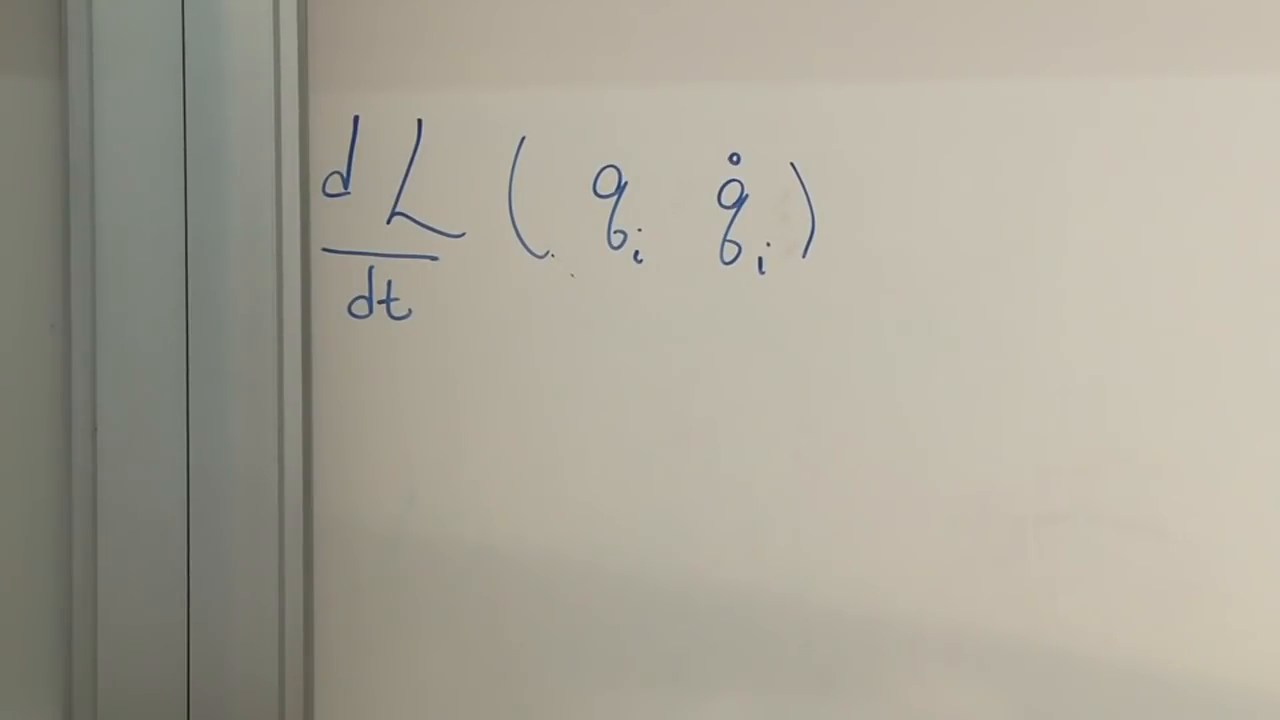
\includegraphics[width=0.72\textwidth]{lecture_05_figure_02.png}
  \caption{開始沿運動軌跡對\(L(q_i,\dot q_i)\)微分。}
  \lectureframe{01:08:51}
\end{figure}

\begin{classroomqa}
  \audiencequestion{鏈鎖律的表示式是不是漏了求和符號？
  \lecturetimestamp{01:10:39--01:11:05}}
  \lecturerresponse{是的。每個座標和每個速度都可能改變拉格朗日量，因此兩項都要對\(i\)求和。}
\end{classroomqa}

使用正則動量與尤拉--拉格朗日方程：
\begin{equation}
  p_i=\frac{\partial L}{\partial\dot q_i},
  \qquad
  \dot p_i=\frac{\partial L}{\partial q_i}.
  \label{eq:l5-p-and-pdot}
\end{equation}
於是式~\eqref{eq:l5-chain-rule-no-time}可寫成
\begin{align}
  \frac{dL}{dt}
  &=\sum_i(\dot p_i\dot q_i+p_i\ddot q_i)
  \notag\\
  &=\frac{d}{dt}\sum_i p_i\dot q_i.
  \label{eq:l5-product-rule}
\end{align}
其中的``巧妙之處''只是乘法法則。

\begin{figure}[htbp]
  \centering
  \includegraphics[width=0.84\textwidth]{lecture_05_figure_21.png}
  \caption{運用運動方程後，鏈鎖律便可改寫為\(\sum_i p_i\dot q_i\)的導數。}
  \lectureframe{01:13:45}
\end{figure}

\begin{classroomqa}
  \audiencequestion{乘積中的最後一個\(q_i\)應該帶一個點，還是兩個點？
  \lecturetimestamp{01:14:31--01:15:32}}
  \lecturerresponse{在乘積中，它是\(p_i\dot q_i\)，只帶一個點。對整個乘積微分會得到
  \(\dot p_i\dot q_i+p_i\ddot q_i\)，所以展開後第二項會出現兩個點。}
\end{classroomqa}

將這兩個導數相減，就得到一個守恆組合。依照歷史慣例，取其負值並稱為哈密頓量：
\begin{equation}
  H=\sum_i p_i\dot q_i-L.
  \label{eq:l5-hamiltonian-definition}
\end{equation}

\begin{figure}[htbp]
  \centering
  \includegraphics[width=0.80\textwidth]{lecture_05_figure_22.png}
  \caption{守恆組合\(L-\sum_i p_i\dot q_i=-H\)與哈密頓量的定義。}
  \lectureframe{01:18:05}
\end{figure}

對於處於勢中的單一粒子，
\begin{equation}
  L=\frac12m\dot x^2-V(x),
  \qquad p=m\dot x.
  \label{eq:l5-particle-lagrangian}
\end{equation}
因此
\begin{align}
  H&=p\dot x-L
  \notag\\
   &=m\dot x^2-\left(\frac12m\dot x^2-V(x)\right)
  \notag\\
   &=\frac12m\dot x^2+V(x)=T+V.
  \label{eq:l5-particle-energy}
\end{align}

\begin{figure}[htbp]
  \centering
  \includegraphics[width=0.86\textwidth]{lecture_05_figure_23.png}
  \caption{處於勢中的粒子，其哈密頓量化為熟悉的動能加勢能。}
  \lectureframe{01:20:50}
\end{figure}

推導過程沒有假設\(L\)必須具有特定形式。因此，在這套形式架構中，能量的一般定義是式~\eqref{eq:l5-hamiltonian-definition}，而不是\(T+V\)。

\section{顯式時間依賴與能量交換}

在鏈鎖律中加入顯式時間依賴：
\begin{equation}
  \frac{dL}{dt}
  =\sum_i\left(
    \frac{\partial L}{\partial q_i}\dot q_i
    +\frac{\partial L}{\partial\dot q_i}\ddot q_i
  \right)
  +\frac{\partial L}{\partial t}.
  \label{eq:l5-full-chain-rule}
\end{equation}
左側是沿著運動軌跡取的全導數。最後的偏導數在\(q\)與\(\dot q\)固定時取值，只對隨外部變化的參數微分。重做同樣的乘法法則步驟，可得
\begin{equation}
  \boxed{\frac{dH}{dt}=-\frac{\partial L}{\partial t}}.
  \label{eq:l5-hamiltonian-time}
\end{equation}

\begin{figure}[htbp]
  \centering
  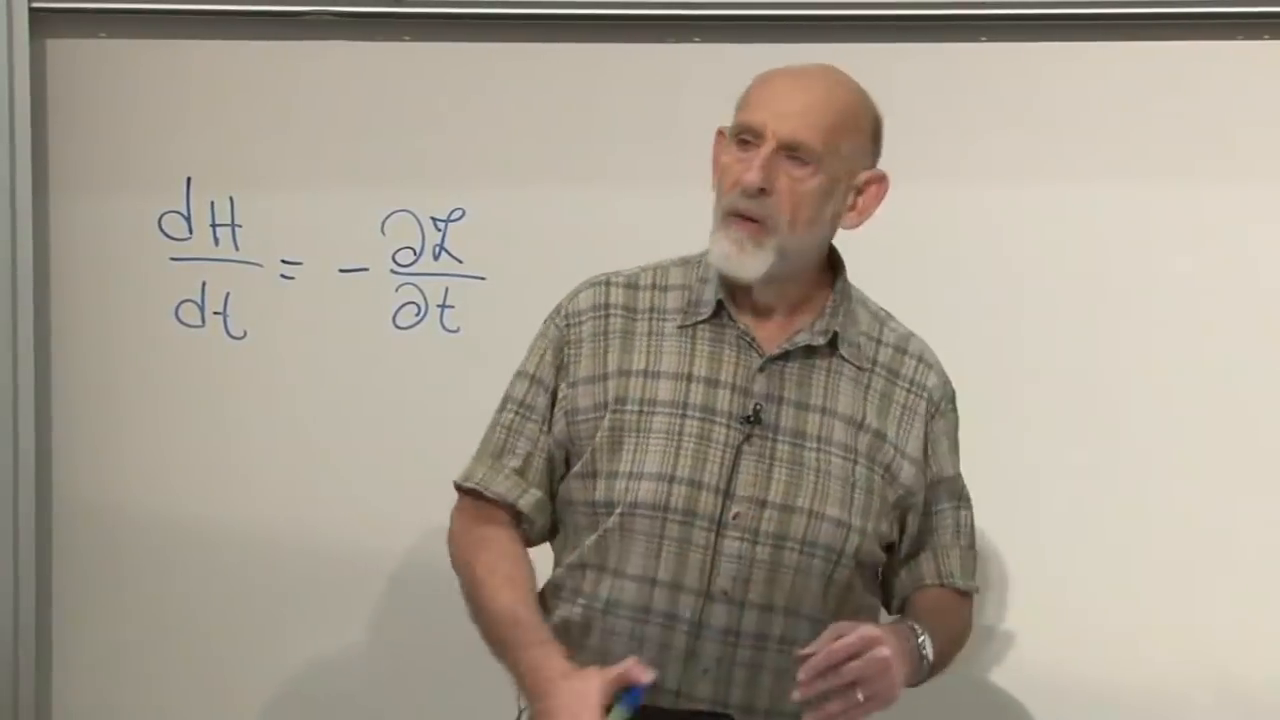
\includegraphics[width=0.70\textwidth]{lecture_05_figure_04.png}
  \caption{哈密頓量的變化只來自拉格朗日量的顯式時間依賴。}
  \lectureframe{01:37:22}
\end{figure}

對於式~\eqref{eq:l5-driven-oscillator}所示的受驅振子，
\begin{equation}
  \frac{\partial L}{\partial t}
  =-\frac12\dot k(t)x^2,
  \qquad
  \dot H=\frac12\dot k(t)x^2.
  \label{eq:l5-driven-energy-rate}
\end{equation}
在\(x=0\)處，瞬時變化率為零；在離開原點的位置，改變彈簧常數所作功的速率正比於\(x^2\dot k\)。

\begin{classroomqa}
  \audiencequestion{若能量不守恆，它的定義是否就是哈密頓量的時間導數？
  \lecturetimestamp{01:27:11--01:28:04}}
  \lecturerresponse{不是。能量就是\(H\)；它的導數則描述能量如何變化。拉格朗日量具有熟悉形式時，\(H=T+V\)；若不是，則由式~\eqref{eq:l5-hamiltonian-definition}定義。將外部驅動器也納入系統後，總哈密頓量便恢復守恆。}
\end{classroomqa}

\begin{classroomqa}
  \audiencequestion{這如何應用到先前那個旋轉木馬上的觀察者？當時出現了離心項與科里奧利項。
  \lecturetimestamp{01:28:08--01:29:52}}
  \lecturerresponse{勻速旋轉的座標系涉及隨時間變化的變數轉換，並非固定的空間對稱性，也不是單純的時間平移。可以從轉換後的拉格朗日量構造哈密頓量，但最好等到討論磁力時再進行這項獨立計算，因為兩者的代數形式十分相近。}
\end{classroomqa}

\section{拉格朗日力學工具一覽}

現在可以將整個架構簡潔地整理如下：
\begin{align}
  L&=L(q_i,\dot q_i,t),
  \notag\\
  p_i&=\frac{\partial L}{\partial\dot q_i},
  \qquad
  \dot p_i=\frac{\partial L}{\partial q_i},
  \notag\\
  \delta q_i&=\epsilon f_i(q)
  \quad\Longrightarrow\quad
  Q=\sum_i p_i f_i(q),\quad \dot Q=0,
  \notag\\
  H&=\sum_i p_i\dot q_i-L,
  \qquad
  \dot H=-\frac{\partial L}{\partial t}.
  \label{eq:l5-toolkit}
\end{align}

\begin{figure}[htbp]
  \centering
  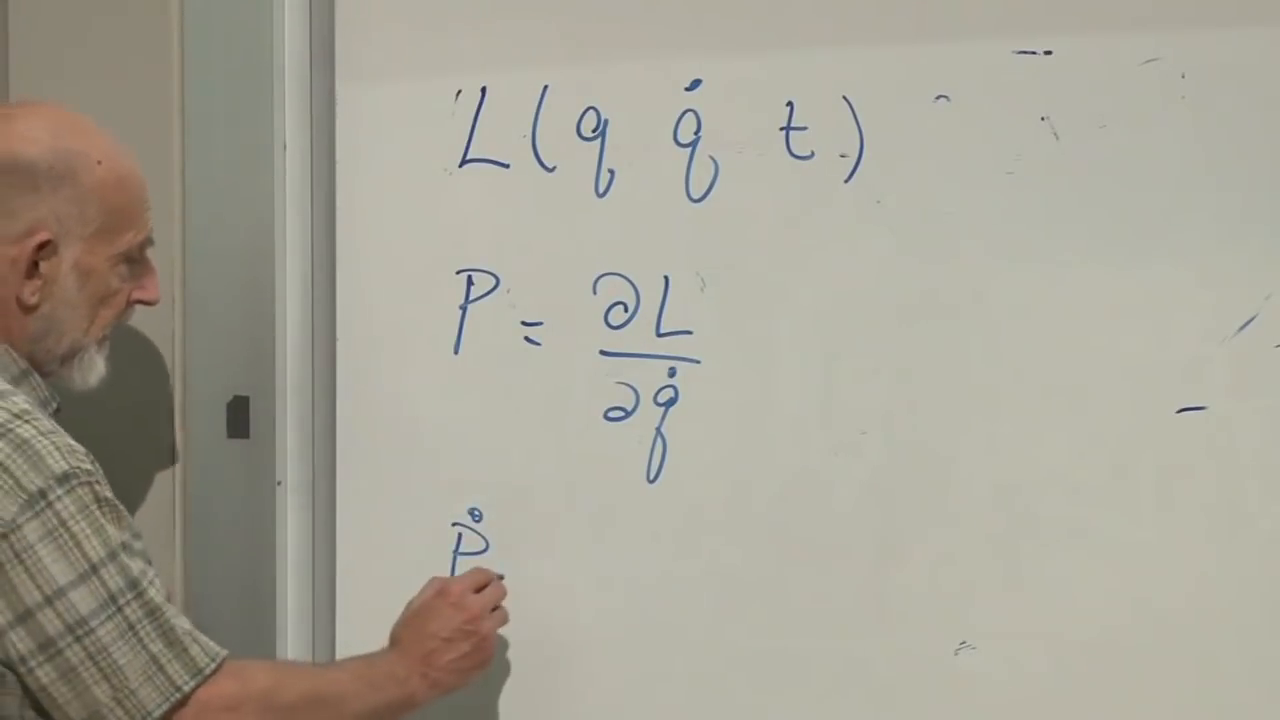
\includegraphics[width=0.66\textwidth]{lecture_05_figure_03.png}
  \caption{板書回顧從\(L(q,\dot q,t)\)、正則動量與尤拉--拉格朗日方程開始。}
  \lectureframe{01:31:37}
\end{figure}

這些公式涵蓋了定義、運動方程、一般連續對稱性所對應的守恆量，以及時間平移所對應的守恆量。需要記住的技巧不多；重要的是能重新推導這些公式，而不是死記彼此無關的表示式。

\section{為什麼要使用拉格朗日力學或哈密頓力學？}

\begin{classroomqa}
  \audiencequestion{力學是否可以同樣用\(L\)或\(H\)來描述？為什麼要選擇其中一種表述？
  \lecturetimestamp{01:37:16--01:39:18}}
  \lecturerresponse{只要勒讓德變換是正則的，兩種表述便等價，但它們著重的結構不同。拉格朗日力學自然地從作用量取駐值出發。哈密頓力學一開始較抽象，但其方程簡潔，且在量子力學中居於核心地位。哈密頓量雖然就是能量，其作用遠不止表達能量守恆。}
\end{classroomqa}

\begin{classroomqa}
  \audiencequestion{牛頓知道能量守恆的哈密頓形式嗎？
  \lecturetimestamp{01:39:29--01:39:56}}
  \lecturerresponse{就歷史記錄所示，牛頓並未使用這種表述。他提出的架構是力定律\(F=ma\)。}
\end{classroomqa}

\begin{classroomqa}
  \audiencequestion{為什麼每個物理系統都應該有拉格朗日量？這只是實驗上的事實嗎？
  \lecturetimestamp{01:39:57--01:42:37}}
  \lecturerresponse{對於此處討論的封閉系統，這是經驗事實，也能從更深層的量子描述導出。數學上自洽、但不是尤拉--拉格朗日方程的微分方程，可以人為構造出來。例如，\(\dot x=-x\)完全可以求解；但若把它當作描述封閉系統的基本單座標定律，它就具有耗散系統那種資訊流失的特徵。經典力學在邏輯上並不先於量子力學；它的基本架構承襲自量子力學。詳細原因留待後續說明。}
\end{classroomqa}

\begin{classroomqa}
  \audiencequestion{如果每個真實的封閉系統都有拉格朗日量，那麼我們稱作拉格朗日量的每個函數，都對應於自然界中實際存在的系統嗎？
  \lecturetimestamp{01:42:39--01:42:54}}
  \lecturerresponse{不是。形式演算容許許多函數，但目前已知的物理系統並未實現其中許多函數。}
\end{classroomqa}

\begin{classroomqa}
  \audiencequestion{拉格朗日量主要是用來發明勢能的工具嗎？
  \lecturetimestamp{01:42:54--01:43:32}}
  \lecturerresponse{它的用途更廣。它可以用來整理可能的力學系統，而且常是導出運動方程最簡便實用的方法。}
\end{classroomqa}

雙擺展現了這種實用上的優勢。選定兩個角度，依據這兩個角度及其時間導數，計算兩個質量的速度，再構造\(T-V\)，讓尤拉--拉格朗日方程以隱含方式處理約束力。這比用\(F=ma\)逐一求解所有張力與加速度，簡潔得多。

\begin{figure}[htbp]
  \centering
  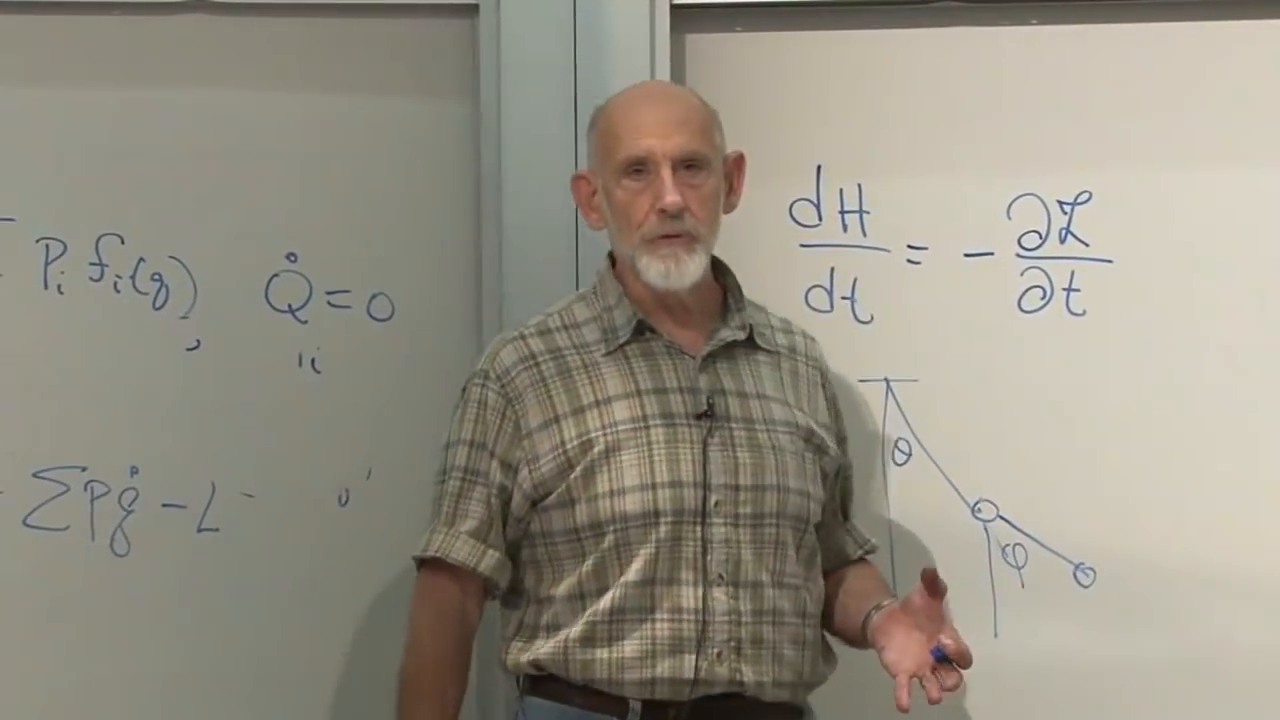
\includegraphics[width=0.84\textwidth]{lecture_05_figure_05.png}
  \caption{能量變化率的恆等式仍寫在黑板上，旁邊是雙擺示意圖。}
  \lectureframe{01:45:39}
\end{figure}

\begin{figure}[htbp]
  \centering
  \begin{tikzpicture}[scale=1.15]
    \draw[thick] (-0.5,0) -- (0.5,0);
    \fill (0,0) circle (0.045);
    \draw[dashed] (0,0) -- (0,-2.3);
    \draw[thick] (0,0) -- (-0.92,-1.22);
    \fill (-0.92,-1.22) circle (0.07);
    \draw[dashed] (-0.92,-1.22) -- (-0.92,-2.55);
    \draw[thick] (-0.92,-1.22) -- (-0.25,-2.18);
    \fill (-0.25,-2.18) circle (0.07);
    \draw (0,-0.55) arc (-90:-127:0.55);
    \node at (-0.42,-0.56) {$\theta$};
    \draw (-0.92,-1.72) arc (-90:-55:0.48);
    \node at (-0.56,-1.72) {$\phi$};
  \end{tikzpicture}
  \caption{雙擺的廣義角座標。}
\end{figure}

變數轉換同樣有效率：先轉換拉格朗日量，再由它導出運動方程，不必分別轉換每一條力方程。

\begin{classroomqa}
  \audiencequestion{雙擺本質上是否也是另一個三體系統，例如太陽、地球和月球，只是把其中一個物體視為錨定物？
  \lecturetimestamp{01:45:06--01:45:25}}
  \lecturerresponse{這個類比點出了兩者的層級關係，雖然桿件施加的是不同約束。在這兩種情況下，都可以在近似中把質量極大或固定的組成部分視為參考結構。}
\end{classroomqa}

\begin{classroomqa}
  \audiencequestion{雙擺採用的是\(T-V\)，但剛才才強調過更一般的拉格朗日量。\(T-V\)在什麼情況下適用？
  \lecturetimestamp{01:46:08--01:46:58}}
  \lecturerresponse{對於在慣性參考系中觀察、且沒有磁性速度耦合的普通非相對論性粒子，這個熟悉的形式適用。旋轉參考系、相對論系統和磁場則需要更一般的項。}
\end{classroomqa}

\begin{classroomqa}
  \audiencequestion{碰撞不屬於這種描述嗎？
  \lecturetimestamp{01:47:00--01:48:05}}
  \lecturerresponse{彈性碰撞源於短程力，因此也可由勢能描述。非彈性碰撞在微觀層次上仍屬於力學現象，但能量會進入內部振動、形變和熱。若質心描述忽略了這些自由度，就不完整。}
\end{classroomqa}

\begin{classroomqa}
  \audiencequestion{棒球被球棒擊中時，可以用\(F=ma\)來分析嗎？
  \lecturetimestamp{01:48:05--01:48:33}}
  \lecturerresponse{只能在粗略的層次上分析。完整的描述必須追蹤形變、升溫、球可能受到的損傷，甚至球棒是否折斷。正因為有這些內部自由度，真實的撞擊才比質點碰撞複雜得多。}
\end{classroomqa}

\begin{classroomqa}
  \audiencequestion{那麼延展的剛體呢？
  \lecturetimestamp{01:48:34--01:49:00}}
  \lecturerresponse{研究剛體可以採用牛頓力學方法，也可以用以平動與轉動座標表示的\(T-V\)拉格朗日量。建構這個拉格朗日量是很好的練習。}
\end{classroomqa}

\begin{classroomqa}
  \audiencequestion{量子力學中的能量--時間不確定性關係，是否意味著能量不會嚴格守恆？
  \lecturetimestamp{01:49:01--01:49:29}}
  \lecturerresponse{不會。能量可以嚴格守恆。這個關係表示，要高精度地測定能量，需要長時間觀測；它並不取代守恆定律。}
\end{classroomqa}

\begin{classroomqa}
  \audiencequestion{牛頓力學與拉格朗日力學在邏輯上等價嗎？
  \lecturetimestamp{01:49:36--01:50:07}}
  \lecturerresponse{在兩種表述都適用的一般範圍內，它們是等價的。不過，也可以構造出某些拉格朗日量，使其方程不像基本形式\(m\ddot x=F(x)\)。}
\end{classroomqa}

\section{座標依賴的動能項}

考慮下面這個刻意選得較不尋常的例子
\begin{equation}
  L=\frac12q^2\dot q^2-\frac12q^2.
  \label{eq:l5-nonstandard-l}
\end{equation}
這是一個有效的拉格朗日量，其中的動能係數依賴座標。也可以考慮速度的一次項，例如\(q\dot q\)；在這個一維例子中，這個特定項是全導數，因此不會改變運動方程。

正則動量為
\begin{equation}
  p=\frac{\partial L}{\partial\dot q}=q^2\dot q,
  \label{eq:l5-nonstandard-p}
\end{equation}
因此
\begin{equation}
  \dot p=q^2\ddot q+2q\dot q^2,
  \qquad
  \frac{\partial L}{\partial q}=q\dot q^2-q.
  \label{eq:l5-nonstandard-derivatives}
\end{equation}
運動方程便是
\begin{equation}
  q^2\ddot q+q\dot q^2=-q.
  \label{eq:l5-nonstandard-eom}
\end{equation}

\begin{figure}[htbp]
  \centering
  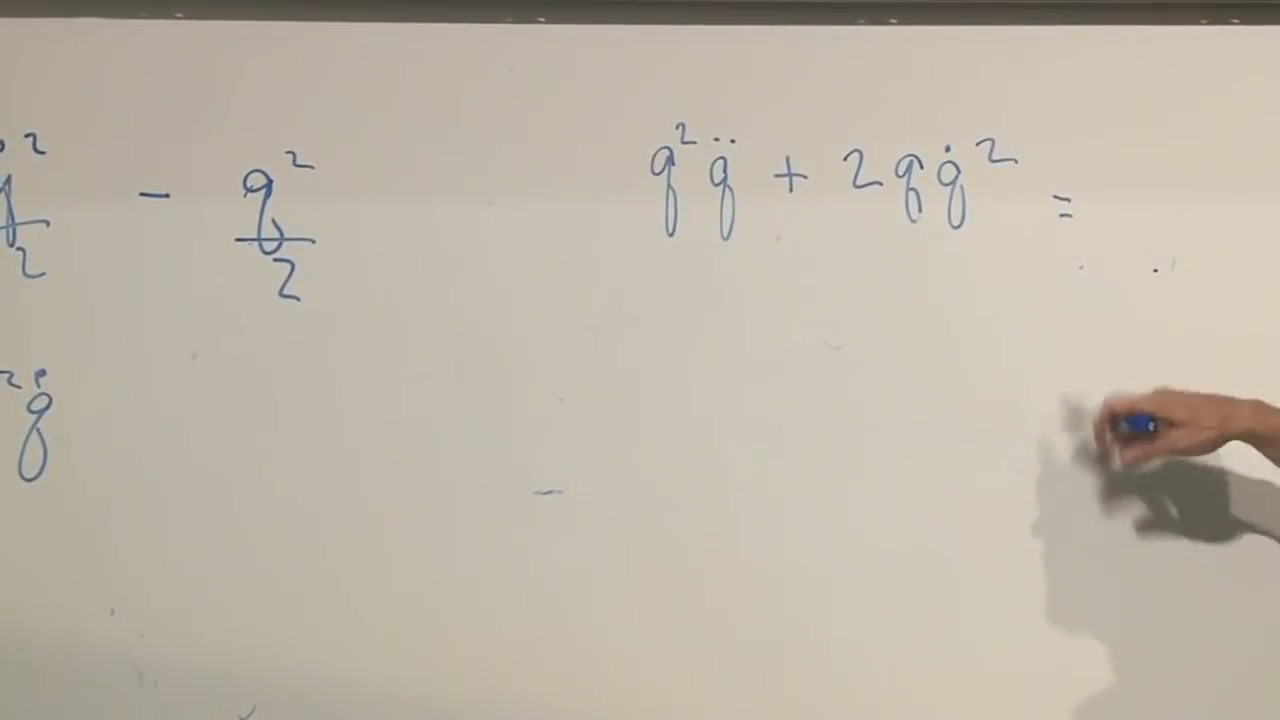
\includegraphics[width=0.80\textwidth]{lecture_05_figure_06.png}
  \caption{座標依賴動能例子中，對動量求導所得的結果。}
  \lectureframe{01:52:32}
\end{figure}

\begin{classroomqa}
  \audiencequestion{可以把方程兩邊除以\(q\)嗎？
  \lecturetimestamp{01:53:22--01:53:39}}
  \lecturerresponse{只有在\(q\neq0\)時才可以。在\(q=0\)時，動能係數與勒讓德映射會退化；若直接相除，就會略過這個必須另行處理的奇異點。}
\end{classroomqa}

哈密頓量為
\begin{align}
  H&=p\dot q-L
  \notag\\
   &=q^2\dot q^2-
     \left(\frac12q^2\dot q^2-\frac12q^2\right)
  \notag\\
   &=\frac12q^2\dot q^2+\frac12q^2.
  \label{eq:l5-nonstandard-h}
\end{align}

\begin{classroomqa}
  \audiencequestion{\(q^2\dot q^2/2\)仍然可以稱為動能嗎？
  \lecturetimestamp{01:54:41--01:55:07}}
  \lecturerresponse{可以。在這個例子中，哈密頓量再次呈現為正的動能項加上勢能項。這裡的重點是，即使事先不假設基本的常質量形式，這些形式定義仍然適用。}
\end{classroomqa}

\section{耗散與形式體系更深層的起源}

\begin{classroomqa}
  \audiencequestion{如何將摩擦納入拉格朗日量？
  \lecturetimestamp{01:55:09--01:56:17}}
  \lecturerresponse{在這裡討論的簡單、封閉且自由度有限的系統中，摩擦並不是以基本力的形式納入的。宏觀摩擦是大量微觀自由度所造成的統計效應。那些原子仍然遵循底層力學，但若約化描述不追蹤它們，就會呈現出耗散。}
\end{classroomqa}

\begin{classroomqa}
  \audiencequestion{哈密頓是如何得出他的表述的？
  \lecturetimestamp{01:56:22--01:56:37}}
  \lecturerresponse{這裡沒有介紹歷史上的推導。對本課程而言，重要的是理解這種表述如何運作。}
\end{classroomqa}

\begin{classroomqa}
  \audiencequestion{若拉格朗日量不明顯地具有\(T-V\)的形式，有沒有更一般的方法可以求得它？
  \lecturetimestamp{01:56:43--01:58:54}}
  \lecturerresponse{實驗、有根據的猜測、對稱性原理，或從期望的方程反推，都可以用來找出這個函數。問微積分本身它的輸入從何而來，就像問導數定義中的\(f(x)\)從何而來一樣。函數一旦指定，微積分就會告訴我們該怎麼做。至於自然界的封閉系統為何符合這種抽象結構，量子力學會從更深的層次給出答案。}
\end{classroomqa}

這一點與本課程開頭談到的主題相連。基本的哈密頓演化具有決定性且可逆；也就是說，軌跡不會合併，資訊也不會就此消失。這項性質與相空間表述的關係，將分階段展開。

\begin{classroomqa}
  \audiencequestion{變分法是否只是從預期的經典方程反向推導而來？量子力學也是用同樣的方法求得拉格朗日量嗎？
  \lecturetimestamp{01:59:37--02:01:07}}
  \lecturerresponse{在初等的經典力學建構中，確實可以選擇一個作用量，使作用量取駐值的路徑重現已知方程。量子力學的邏輯順序則不同：它自然地從哈密頓量出發，再進一步導出拉格朗日描述。哈密頓量在量子力學中更為直觀，雖然它在經典力學中初看之下較為抽象。}
\end{classroomqa}

\begin{classroomqa}
  \audiencequestion{量子力學能描述摩擦嗎？
  \lecturetimestamp{02:01:08--02:02:05}}
  \lecturerresponse{可以，但基本描述必須納入環境的自由度。若不考慮流體中的粒子，就無法完整描述在黏性流體中運動的粒子。當這些自由度沒有逐一追蹤時，摩擦便是隨之湧現的複雜集體效應。}
\end{classroomqa}

\chapter{受約束系統與哈密頓運動}

\lectureoverview{兩個受約束系統展現了拉格朗日力學為何如此有效：選定適當座標後，無須明確計算約束力，就能寫出運動方程及其守恆律。同樣的例子接著引出哈密頓力學：座標與動量構成相空間，諧振子化為剛性旋轉，而哈密頓的兩個一階方程則取代每個二階的尤拉--拉格朗日方程。}

\section{求解力學問題的意義}

拉格朗日方法的直接目的在於實用。楔塊在地面上滑動、雙擺運動，兩者都能用牛頓定律處理，但未知的接觸力與張力很快就會讓計算變得繁瑣。掌握拉格朗日力學的規則後，同樣的問題便能化為一連串有條理的步驟：
\begin{enumerate}
  \item 選取能標示瞬時位形的獨立座標；
  \item 用這些座標表示動能與勢能；
  \item 構造\(L=T-V\)，並套用尤拉--拉格朗日方程。
\end{enumerate}

就此處的目的而言，只要正確寫出運動方程，問題就算已經\emph{解決}。或許還想求出閉合形式的軌跡，但那是另一回事。力學設定完成後，非線性微分方程可以用數值方法積分。困難之處往往不在積分，而在於找出能納入約束、又不引進冗餘未知力的變數。

\section{在移動的楔塊上滑動的質點}

考慮一個質量為\(M\)的楔塊，受約束而無摩擦地沿水平面滑動。另一個質量為\(m\)的質點則受約束，沿著斜面移動。這個系統有兩個自由度：一個表示楔塊的位置，另一個表示質點在楔塊上的位置。

令
\begin{equation}
  \begin{aligned}
    X&=\text{horizontal position of the wedge corner},\\
    x&=\text{horizontal displacement of the particle}\\[-0.2em]
     &\phantom{={}}\text{from that corner}.
  \end{aligned}
  \label{eq:l6-wedge-coordinates}
\end{equation}
因此，質點的絕對水平座標為\(X+x\)。座標的選法並不唯一；也可以改用沿斜面的距離，或質點的絕對水平座標。只要一組座標不冗餘，且能標示相同的位形，就是合法的選擇；不過，有些選法比其他選法更能清楚呈現系統的結構。

斜面角\(\beta\)固定時，垂直位移\(y\)不是獨立座標：
\begin{equation}
  y=x\tan\beta,
  \qquad
  \dot y=\dot x\tan\beta.
  \label{eq:l6-wedge-constraint}
\end{equation}
我們特別取\(\beta=45^\circ\)，因此\(y=x\)，且
\(\dot y=\dot x\)。這項簡化省去了三角函數因子，但不影響這個例子的要旨。

\begin{figure}[htbp]
  \centering
  \includegraphics[width=0.84\textwidth]{lecture_06_figure_06.png}
  \caption{移動的楔塊、受約束的質點，以及\(45^\circ\)例子中使用的水平與垂直速度分量。}
  \lectureframe{00:10:25}
\end{figure}

楔塊的動能為
\begin{equation}
  T_{M}=\frac{M}{2}\dot X^2.
  \label{eq:l6-wedge-kinetic}
\end{equation}
質點的水平速度為\(\dot X+\dot x\)，垂直速度則為\(\dot x\)。因此，質點的動能為
\begin{equation}
  T_m=\frac{m}{2}\left[(\dot X+\dot x)^2+\dot x^2\right].
  \label{eq:l6-particle-kinetic}
\end{equation}
以\(x=0\)為重力位能的零點，則\(V=mgx\)。所以
\begin{equation}
  L=\frac{M}{2}\dot X^2
    +\frac{m}{2}\left[(\dot X+\dot x)^2+\dot x^2\right]
    -mgx.
  \label{eq:l6-wedge-lagrangian}
\end{equation}

\begin{figure}[htbp]
  \centering
  \includegraphics[width=0.86\textwidth]{lecture_06_figure_07.png}
  \caption{楔塊的幾何、\(V=mgx\)，以及彙整在黑板上的兩項動能。}
  \lectureframe{00:14:15}
\end{figure}

\subsection{正則動量由拉格朗日量定義}

正則動量是由拉格朗日量定義的，不能只憑單一質點的速度來猜：
\begin{align}
  p_X&=\frac{\partial L}{\partial\dot X}
      =M\dot X+m(\dot X+\dot x),
      \label{eq:l6-wedge-pX}\\
  p_x&=\frac{\partial L}{\partial\dot x}
      =m(\dot X+\dot x)+m\dot x.
      \label{eq:l6-wedge-px}
\end{align}
第一個表式就是一般所說的總水平動量：楔塊貢獻\(M\dot X\)，質點貢獻\(m(\dot X+\dot x)\)。在此，它是與座標\(X\)共軛的動量。

\begin{figure}[htbp]
  \centering
  \includegraphics[width=0.86\textwidth]{lecture_06_figure_08.png}
  \caption{分別與楔塊座標\(X\)及質點相對座標\(x\)共軛的正則動量。}
  \lectureframe{00:18:05}
\end{figure}

拉格朗日量沒有明確依賴\(X\)。整個裝置的水平平移變換為
\begin{equation}
  \delta X=\epsilon,
  \qquad
  \delta x=0.
  \label{eq:l6-wedge-translation}
\end{equation}
因此，套用一般的無窮小對稱性規則
\begin{equation}
  \delta q_i=\epsilon f_i(q),
  \qquad
  Q=\sum_i p_i f_i
  \label{eq:l6-noether-rule}
\end{equation}
可得\(Q=p_X\)。換言之，\(X\)是循環座標，而且
\begin{equation}
  \dot p_X=\frac{\partial L}{\partial X}=0.
  \label{eq:l6-wedge-conservation}
\end{equation}

系統沒有相應的垂直平移對稱性。楔塊不能垂直移動，而改變質點的高度會改變重力位能。因此，水平動量守恆；這個受約束子系統的垂直動量則不守恆。

對相對座標而言，尤拉--拉格朗日方程為
\begin{equation}
  \dot p_x=\frac{\partial L}{\partial x}=-mg.
  \label{eq:l6-wedge-force}
\end{equation}
黑板上的這一行曾修正過符號。可靠的推導方式是從\(L=T-V\)出發：由於\(V=mgx\)，拉格朗日量對該座標的導數為\(-mg\)。\(x\)雖然是以水平位移引入的，重力仍會出現在它的方程中，因為約束將這個水平位移與垂直高度\(y=x\)連結起來。

這裡沒有出現法向力或反作用力。這些力會自動取適當的值，以維持約束。牛頓方法會把它們列入，並與加速度一併求解；使用廣義座標便不必處理這些力。

\section{雙擺與座標的巧妙選擇}

現在將兩個單位質量懸掛在兩根無質量、長度為一的桿上。第一根桿與鉛直向下方向的夾角為\(\theta\)。第二個自由度有兩種選擇：使用第二個絕對角\(\phi\)，或使用兩根桿之間的相對角\(\alpha\)。

相對角是較能揭示系統特性的選擇。暫時關閉重力。整個裝置的剛性旋轉會改變絕對取向，卻不改變兩根桿的夾角：
\begin{equation}
  \theta\longrightarrow\theta+\epsilon,
  \qquad
  \alpha\longrightarrow\alpha.
  \label{eq:l6-double-rotation}
\end{equation}
採用這種座標選擇後，旋轉對稱變換只作用在一個座標上。這不表示其他座標系有誤；這樣選只是讓對稱性，以及由此而來的守恆量，更容易看出。

\begin{figure}[htbp]
  \centering
  \includegraphics[width=0.76\textwidth]{lecture_06_figure_09.png}
  \caption{雙擺以\(\theta\)表示第一個絕對角，並以\(\alpha\)表示第二根桿相對於第一根桿的角度。}
  \lectureframe{00:29:20}
\end{figure}

為了求出動能，可以暫時用笛卡兒座標輔助計算。令垂直座標向下為正，第一個擺錘的位置為
\begin{equation}
  x_1=\sin\theta,
  \qquad
  y_1=\cos\theta,
  \label{eq:l6-bob-one-position}
\end{equation}
因此
\begin{equation}
  \dot x_1=\dot\theta\cos\theta,
  \qquad
  \dot y_1=-\dot\theta\sin\theta,
  \qquad
  \dot x_1^2+\dot y_1^2=\dot\theta^2.
  \label{eq:l6-bob-one-velocity}
\end{equation}
第二個擺錘的位置為
\begin{align}
  x_2&=\sin\theta+\sin(\theta+\alpha),\\
  y_2&=\cos\theta+\cos(\theta+\alpha),
  \label{eq:l6-bob-two-position}
\end{align}
例如，
\begin{equation}
  \dot x_2=\dot\theta\cos\theta
  +(\dot\theta+\dot\alpha)\cos(\theta+\alpha),
  \label{eq:l6-bob-two-xvelocity}
\end{equation}
而\(\dot y_2\)也有類似的表式。

\begin{figure}[htbp]
  \centering
  \includegraphics[width=0.88\textwidth]{lecture_06_figure_10.png}
  \caption{兩個擺錘的輔助笛卡兒座標。這些座標用來計算速度，並未作為額外自由度引入。}
  \lectureframe{00:35:25}
\end{figure}

將兩個動能相加，可得下列結果。交叉項來自
\begin{equation*}
  \cos A\cos B+\sin A\sin B=\cos(A-B).
\end{equation*}
\begin{equation}
  T=\dot\theta^2
    +\frac12(\dot\theta+\dot\alpha)^2
    +\dot\theta(\dot\theta+\dot\alpha)\cos\alpha.
  \label{eq:l6-double-kinetic}
\end{equation}

\begin{classroomqa}
  \audiencequestion{這個表式已包含兩個擺錘的動能嗎？是不是少了一個二分之一因子？
  \lecturetimestamp{00:38:06--00:38:27}}
  \lecturerresponse{兩者都包含在內。這個表式來自
  \(\tfrac12(\dot x_1^2+\dot y_1^2+\dot x_2^2+\dot y_2^2)\)。
  兩個相同的貢獻相加後，形成第一項\(\dot\theta^2\)；沒有少掉任何因子。}
\end{classroomqa}

沒有重力時，\(L=T\)不顯含\(\theta\)。因此
\begin{equation}
  \dot p_\theta=\frac{\partial L}{\partial\theta}=0,
  \label{eq:l6-double-angular-conservation}
\end{equation}
而\(p_\theta\)就是總角動量。要注意「沒有出現\(\theta\)」的確切意思：\(\dot\theta\)當然會出現，但未微分的座標本身並未出現。

恢復重力後，整體旋轉對稱性便遭到破壞。採用上述垂直向下的座標約定，並選取一個方便的零點，可得
\begin{equation}
  V=-g(y_1+y_2)
   =-g\left[2\cos\theta+\cos(\theta+\alpha)\right].
  \label{eq:l6-double-potential}
\end{equation}
加上一個常數不會造成影響。要點是\(\theta\)現在明確出現在式中，因此它的共軛動量不再守恆。能量仍然守恆，因為拉格朗日量沒有明確依賴時間。

\begin{classroomqa}
  \audiencequestion{黑板上的\(\dot\theta-\dot\alpha\)是否應該寫成\(\dot\theta+\dot\alpha\)？
  \lecturetimestamp{00:43:00--00:43:54}}
  \lecturerresponse{依照這裡採用的取向，應使用正號。這是式~\eqref{eq:l6-bob-two-position}採用的約定，並延續至式~\eqref{eq:l6-double-kinetic}的動能中。若反轉正\(\alpha\)的定義，相應的符號也會改變，但所有出現處都必須一致更改。黑板上的寫法混用了兩種約定。}
\end{classroomqa}

\begin{figure}[htbp]
  \centering
  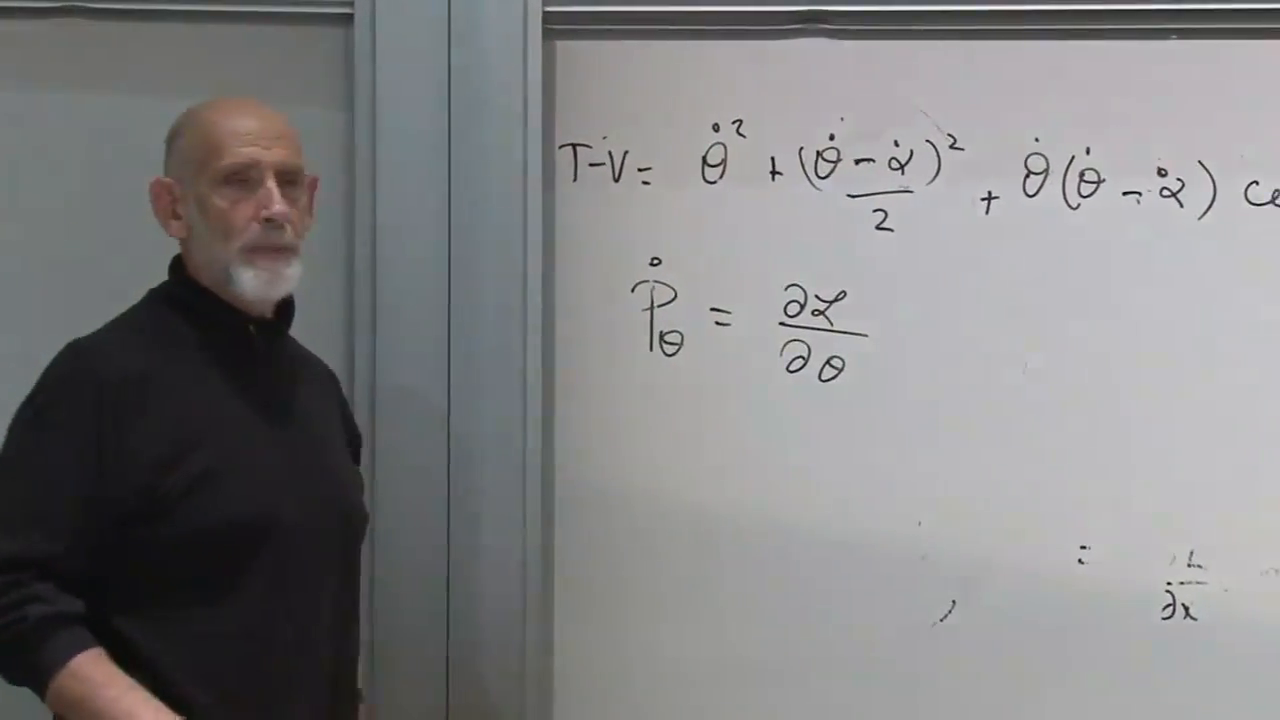
\includegraphics[width=0.84\textwidth]{lecture_06_figure_02.png}
  \caption{無重力時的擺系統計算，以及\(\dot p_\theta=\partial L/\partial\theta\)。上方黑板行列出的是問題中提到、符號不一致的局部記號；整理後的公式見式~\eqref{eq:l6-double-kinetic}。}
  \lectureframe{00:45:50}
\end{figure}

知道\(T\)與\(V\)後，其餘方程便可透過微分求得。桿的張力以及維持桿長固定的力，再次因座標的選擇而不必明確處理。

\subsection{守恆的意義與限度}

\begin{classroomqa}
  \audiencequestion{能否直接從方程看出雙擺是否具有混沌行為？
  \lecturetimestamp{00:44:57--00:45:25}}
  \lecturerresponse{通常無法只靠簡單觀察判斷。系統可能隨著參數或能量的變化，從規則運動轉為混沌運動。要探討這個問題，需要比方程表面形式更完整的架構，後面會再談到。}
\end{classroomqa}

\begin{classroomqa}
  \audiencequestion{在保守系統中，每個\(\dot p_i\)都等於零嗎？
  \lecturetimestamp{00:45:25--00:46:24}}
  \lecturerresponse{不一定。一般方程是
  \(\dot p_i=\partial L/\partial q_i\)。只有當\(q_i\)是循環座標時，它才會為零。循環座標是特別簡單的情況：透過對稱變換使一個座標平移，同時其他座標保持不變。}
\end{classroomqa}

如果唯一的目標是進行數值演化，即使座標系不方便，也仍然可行；只是方程會更長。巧妙選擇座標的好處在於概念上的清晰：還沒解方程，就已經能看出哪個動量守恆。

\begin{classroomqa}
  \audiencequestion{沒有重力時，雙擺的運動會像單一自由擺那樣簡單嗎？
  \lecturetimestamp{00:47:02--00:47:35}}
  \lecturerresponse{單一自由轉子會等角速度轉動，因為它的角動量決定了運動。雙擺即使保持總角動量守恆，相對運動仍可能十分複雜。若兩個角速度初始都為零，系統便保持靜止；否則兩部分會相互作用。}
\end{classroomqa}

\begin{classroomqa}
  \audiencequestion{沒有重力時，\(\dot\theta\)與\(\dot\alpha\)各自會保持不變嗎？
  \lecturetimestamp{00:47:36--00:52:42}}
  \lecturerresponse{不會。守恆表示\(\dot p_\theta=0\)，而不是\(\ddot\theta=0\)或\(\ddot\alpha=0\)。\(p_\theta=\partial L/\partial\dot\theta\)的表式包含兩個角速度，且取決於\(\alpha\)。桿會傳遞力矩，使兩個擺錘得以交換角動量與能量。這類似以彈簧連接的兩個質點：總動量與質心速度保持不變，但各質點的速度會振盪。對應的轉動量是某個特定的集體組合，而不是任一角度本身。}
\end{classroomqa}

\begin{classroomqa}
  \audiencequestion{交換角動量的力是透過桿傳遞的嗎？
  \lecturetimestamp{00:52:43--00:53:34}}
  \lecturerresponse{是。沿桿傳遞的力不一定通過另一個運動所繞的支點，因此可能對該支點產生力矩。力矩就是力使物體轉動的效應；在這裡，它造成各自非零的角加速度。}
\end{classroomqa}

\section{作為第三種力學表述的哈密頓量}

哈密頓量就是能量，但這只是它的第一層意義。它也是第三種力學表述的基礎。牛頓方程以力和加速度描述運動；駐作用量原理則導出尤拉--拉格朗日方程。對於正則系統，哈密頓力學與後者等價，但使用的變數與幾何觀點不同。

改用\(q_i\)與其共軛動量\(p_i\)，而不使用\(q_i\)和\(\dot q_i\)。具有\(n\)個自由度的系統，無論採用哪種描述，都需要\(2n\)個數來表示狀態：可以是位置與速度，也可以是位置與動量。兩者之間的連結是
\begin{equation}
  p_i=\frac{\partial L}{\partial\dot q_i}.
  \label{eq:l6-legendre-map}
\end{equation}
若這些關係可以反解出速度\(\dot q_i(q,p)\)，便定義
\begin{equation}
  H(q,p)=\sum_i p_i\dot q_i-L(q,\dot q).
  \label{eq:l6-hamiltonian-definition}
\end{equation}
如此一來，右側的速度便可消去，改以\(q\)和\(p\)表示。這種可逆性就是正則勒讓德變換所需的假設。奇異拉格朗日量則需要更一般的約束理論；這種初等構造不適用於它們。

\subsection{微積分之前先談可逆性}

回想一組以箭頭連結的有限個抽象狀態。若兩個較早的狀態都演變到同一個較晚的狀態，確定性規則仍可能不可逆：未來是唯一的，過去卻不唯一。若將所有箭頭反向，則會出現相反的問題：一個狀態分岔出多個未來。前一種圖中箭頭匯聚，後一種圖中箭頭發散。

\begin{figure}[htbp]
  \centering
  \includegraphics[width=0.86\textwidth]{lecture_06_figure_11.png}
  \caption{用來對照可逆循環，以及不允許的匯聚與發散之抽象狀態映射。}
  \lectureframe{00:56:20}
\end{figure}

哈密頓流將為這個說法提供連續版本。相空間中的一團點可以移動、變形，但不會形成消除狀態差異的匯，也不會形成從單一狀態產生多個未來的源。證明留待後續；目前先由這些圖示引出幾何觀點。

\begin{classroomqa}
  \audiencequestion{這張抽象狀態圖是否應解讀為物體在重力場中運動？
  \lecturetimestamp{00:58:02--00:58:35}}
  \lecturerresponse{不是。圖中的點只是抽象狀態，箭頭則表示狀態變化的規則。這張圖沒有任何空間或重力上的意義。}
\end{classroomqa}

\begin{classroomqa}
  \audiencequestion{要如何區分不允許的收斂狀態映射與黑洞？
  \lecturetimestamp{00:58:40--00:59:28}}
  \lecturerresponse{這需要非常細緻的分析。這個問題問得合理，但要正確回答，必須仔細描述完整狀態及其量子引力演化。單靠這張簡單圖示不足以判定。}
\end{classroomqa}

\section{適合相空間描述的振子}

在推導一般方程之前，先考慮一個刻意採用適合相空間變數來表示的諧振子：
\begin{equation}
  L=\frac{1}{2\omega}\dot q^2-\frac{\omega}{2}q^2.
  \label{eq:l6-rescaled-lagrangian}
\end{equation}
其共軛動量為
\begin{equation}
  p=\frac{\partial L}{\partial\dot q}=\frac{\dot q}{\omega},
  \qquad
  \dot q=\omega p.
  \label{eq:l6-rescaled-momentum}
\end{equation}
代入式~\eqref{eq:l6-hamiltonian-definition}，可得
\begin{align}
  H&=p\dot q-L\\
   &=\omega p^2-\frac{\omega p^2}{2}+\frac{\omega q^2}{2}
    =\frac{\omega}{2}(p^2+q^2).
  \label{eq:l6-oscillator-hamiltonian}
\end{align}

\begin{figure}[htbp]
  \centering
  \includegraphics[width=0.86\textwidth]{lecture_06_figure_12.png}
  \caption{適配振子的勒讓德變換，以及對稱形式的哈密頓量\(H=\tfrac{\omega}{2}(p^2+q^2)\)。}
  \lectureframe{01:08:20}
\end{figure}

\(q\)與\(p\)構成的空間就是相空間。一個自由度對應二維平面；兩個自由度則對應四維相空間。振子能量固定時，
\begin{equation}
  p^2+q^2=\frac{2H}{\omega},
  \label{eq:l6-energy-circle}
\end{equation}
所以軌跡會保持在圓上。能量守恆將運動限制在其中一條曲線上。

\begin{figure}[htbp]
  \centering
  \includegraphics[width=0.82\textwidth]{lecture_06_figure_13.png}
  \caption{振子相平面中的巢狀等能圓；\(q\)為水平軸，\(p\)為垂直軸。}
  \lectureframe{01:13:20}
\end{figure}

\section{推導哈密頓方程}

這項推導是多變數函數微分的練習。對於\(F(q,p)\)，
\begin{equation}
  \delta F=\sum_i\left(
  \frac{\partial F}{\partial q_i}\delta q_i
  +\frac{\partial F}{\partial p_i}\delta p_i\right).
  \label{eq:l6-total-differential}
\end{equation}
從不同方向都能讀出係數：\(\delta q_i\)的係數是\(\partial F/\partial q_i\)，而\(\delta p_i\)的係數是\(\partial F/\partial p_i\)。

現在對\(H\)的定義式取變分：
\begin{align}
  \delta H
  &=\sum_i\left(\dot q_i\,\delta p_i
       +p_i\,\delta\dot q_i\right)-\delta L\\
  &=\sum_i\left(\dot q_i\,\delta p_i
       +p_i\,\delta\dot q_i
       -\frac{\partial L}{\partial q_i}\delta q_i
       -\frac{\partial L}{\partial\dot q_i}\delta\dot q_i\right).
  \label{eq:l6-vary-hamiltonian}
\end{align}
由於\(\partial L/\partial\dot q_i=p_i\)，兩個\(\delta\dot q_i\)項會相消。尤拉--拉格朗日方程給出\(\partial L/\partial q_i=\dot p_i\)，剩下
\begin{equation}
  \delta H=\sum_i\left(\dot q_i\,\delta p_i
                     -\dot p_i\,\delta q_i\right).
  \label{eq:l6-reduced-variation}
\end{equation}

\begin{figure}[htbp]
  \centering
  \includegraphics[width=0.86\textwidth]{lecture_06_figure_14.png}
  \caption{\(\delta H\)依乘積法則展開後、\(p_i\,\delta\dot q_i\)項相消之前的形式。}
  \lectureframe{01:18:40}
\end{figure}

比較式~\eqref{eq:l6-reduced-variation}與式~\eqref{eq:l6-total-differential}的一般微分式，對照獨立係數即可得到哈密頓方程：
\begin{equation}
  \boxed{
  \dot q_i=\frac{\partial H}{\partial p_i},
  \qquad
  \dot p_i=-\frac{\partial H}{\partial q_i}.}
  \label{eq:l6-hamilton-equations}
\end{equation}

\begin{figure}[htbp]
  \centering
  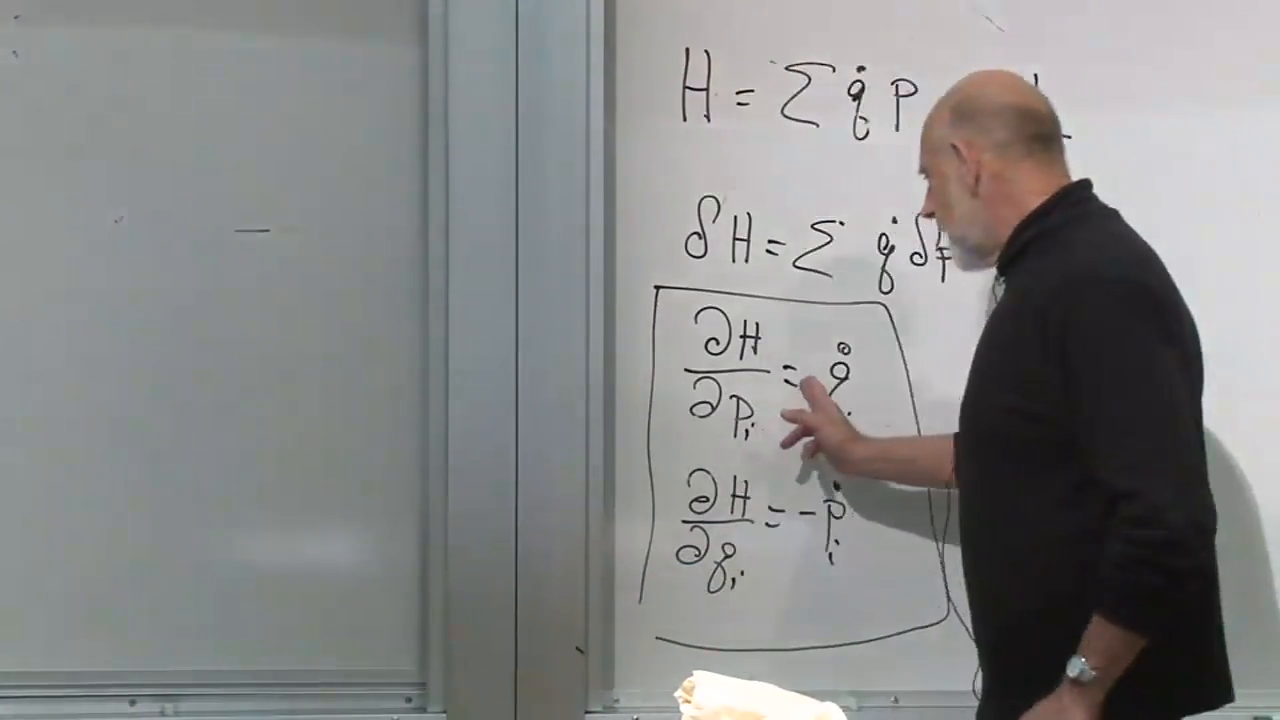
\includegraphics[width=0.78\textwidth]{lecture_06_figure_03.png}
  \caption{哈密頓量的定義、其變分，以及框列的正則方程。}
  \lectureframe{01:22:18}
\end{figure}

對\(n\)個座標而言，這是\(2n\)個一階方程。尤拉--拉格朗日表述則提供\(n\)個二階方程。兩種表述所需的初始資料數量相同，物理內容也完全相同。

\section{振子運動就是剛性旋轉}

將式~\eqref{eq:l6-hamilton-equations}套用於式~\eqref{eq:l6-oscillator-hamiltonian}，可得
\begin{equation}
  \dot q=\omega p,
  \qquad
  \dot p=-\omega q.
  \label{eq:l6-oscillator-first-order}
\end{equation}
對第一個方程微分，再利用第二個方程，得到
\begin{equation}
  \ddot q=\omega\dot p=-\omega^2q.
  \label{eq:l6-oscillator-second-order}
\end{equation}
因此，這兩個一階方程恰好等同於通常的二階振子方程，並包含動量的定義。

在相空間中，\((q,p)\)處的速度向量為\((\dot q,\dot p)=(\omega p,-\omega q)\)，與等能圓相切。每條半徑都以相同的角速度\(\omega\)旋轉。整個平面可以想成剛性的風車，也可以想成不可壓縮的虛構流體。平面上的點會循環流動，不會擠入某個匯，也不會從某個源向外發散。

\begin{figure}[htbp]
  \centering
  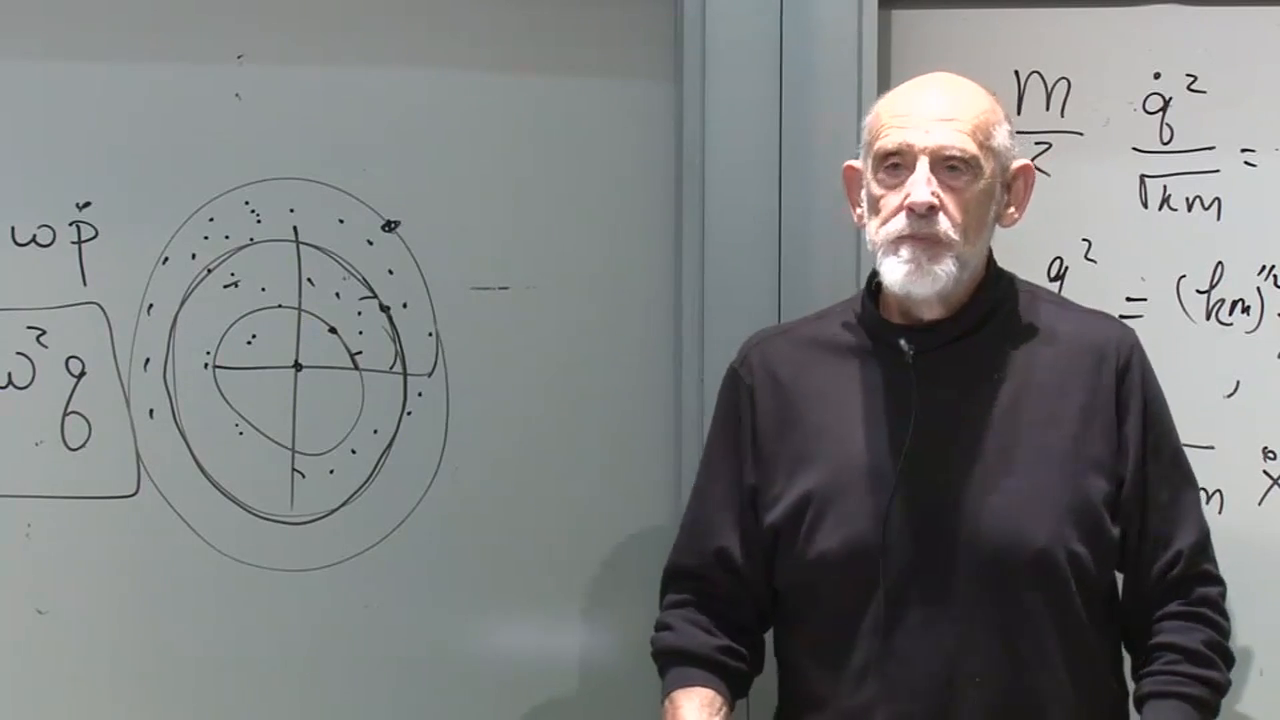
\includegraphics[width=0.86\textwidth]{lecture_06_figure_04.png}
  \caption{一團初始點分布在巢狀的相空間軌跡上。哈密頓演化會帶動這團點，而不會使它塌縮到某個偏好的狀態。}
  \lectureframe{01:39:27}
\end{figure}

\begin{figure}[htbp]
  \centering
  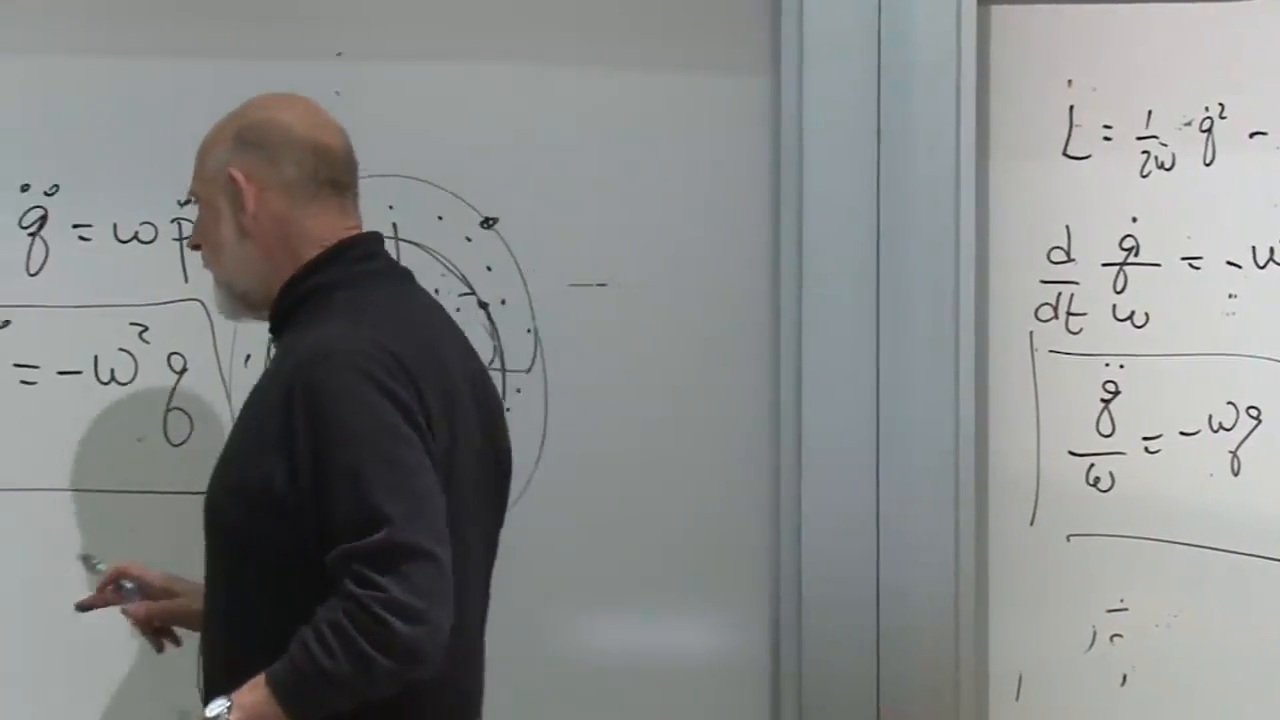
\includegraphics[width=0.90\textwidth]{lecture_06_figure_05.png}
  \caption{振子相圖，旁列等價的尤拉--拉格朗日方程\(\ddot q/\omega=-\omega q\)。}
  \lectureframe{01:42:10}
\end{figure}

下一步會將流體類比嚴格化為定理：哈密頓流在局部不會收斂或發散。這個結果會把連續力學與課程開頭討論的可逆狀態映射重新連結起來。

\section{從座標選擇引出的問題}

\begin{classroomqa}
  \audiencequestion{速度可以用\(q\)和\(p\)求解，這項假設究竟是定理，還是物理系統的經驗性質？
  \lecturetimestamp{01:29:08--01:29:45}}
  \lecturerresponse{在這套初等推導中，這是一項經驗規律，其更深層的動機來自量子力學。更精確地說，式~\eqref{eq:l6-legendre-map}對速度的雅可比矩陣必須非奇異。現代力學也包含重要的奇異拉格朗日量，尤其是受約束系統與規範系統；但其哈密頓表述需要額外的約束處理架構。}
\end{classroomqa}

對量綱的疑問可以說明，為什麼振子會寫成式~\eqref{eq:l6-rescaled-lagrangian}中不熟悉的形式。先從一般座標\(x\)出發：
\begin{equation}
  L=\frac{m}{2}\dot x^2-\frac{k}{2}x^2,
  \qquad
  \omega=\sqrt{\frac{k}{m}}.
  \label{eq:l6-ordinary-oscillator}
\end{equation}
令
\begin{equation}
  q=(km)^{1/4}x.
  \label{eq:l6-oscillator-rescaling}
\end{equation}
於是\(q^2=\sqrt{km}\,x^2\)且\(\dot q^2=\sqrt{km}\,\dot x^2\)，式~\eqref{eq:l6-ordinary-oscillator}便恰好轉換為式~\eqref{eq:l6-rescaled-lagrangian}。新的\(q\)是經過調整的廣義座標，不是長度；它的共軛動量\(p\)也不是一般的力學動量\(p_x=m\dot x\)。

\begin{figure}[htbp]
  \centering
  \includegraphics[width=0.86\textwidth]{lecture_06_figure_15.png}
  \caption{從一般振子座標\(x\)到調整後座標\(q=(km)^{1/4}x\)的量綱重標度。}
  \lectureframe{01:36:10}
\end{figure}

\begin{classroomqa}
  \audiencequestion{\(\omega p=\dot q\)如何符合量綱一致性？為什麼要選用這些變數？
  \lecturetimestamp{01:29:46--01:39:22}}
  \lecturerresponse{符號\(q\)不必具有長度量綱，其共軛動量\(p\)也不必具有\(m\dot x\)的量綱。式~\eqref{eq:l6-oscillator-rescaling}中的重標度保留了拉格朗日量的量綱，並使\(q\)與\(p\)對稱地出現在\(H\)中。在原來的變數中，
  \[
    H=\frac{p_x^2}{2m}+\frac{kx^2}{2},
  \]
  因此，\((x,p_x)\)平面上的等能曲線是橢圓；在調整後的\((q,p)\)平面上則是圓。選用這種重標度，就是為了凸顯這項對稱性。}
\end{classroomqa}

\begin{classroomqa}
  \audiencequestion{\(2n\)個一階哈密頓方程，怎麼會等價於\(n\)個二階拉格朗日方程？
  \lecturetimestamp{01:39:24--01:42:30}}
  \lecturerresponse{對振子而言，將\(\dot q=\omega p\)微分並代入\(\dot p=-\omega q\)，這一對方程便化為\(\ddot q=-\omega^2q\)。若直接從拉格朗日量出發，則得到
  \[
    \frac{d}{dt}\left(\frac{\dot q}{\omega}\right)
      =-\omega q,
  \]
這是相同的二階方程。一個哈密頓方程可視為以速度定義動量，另一個則描述該動量如何演化。}
\end{classroomqa}

\section{相空間與位能為何重要}

\begin{classroomqa}
  \audiencequestion{哈密頓量的強大作用，是否表示相空間在幾何表述上優於位形空間？
  \lecturetimestamp{01:42:33--01:44:38}}
  \lecturerresponse{兩者用途不同。相空間能格外清楚地呈現循環、等能面，以及沒有收斂或發散的特性；位形空間則可能更適合探討其他問題。重視\(H\)更深層的原因在於，它在量子力學中會成為核心且更直觀的對象，而量子力學正是這套力學所引向的現代學科之一。}
\end{classroomqa}

\begin{classroomqa}
  \audiencequestion{勢能應視為力的積分嗎？
  \lecturetimestamp{01:44:40--01:45:45}}
  \lecturerresponse{對保守力而言，這種說法成立，但須相差一個常數，且符號要適當。更實用的做法是將勢能視為基本量，再由它導出廣義力：
  \[
    F_i=-\frac{\partial V}{\partial q_i}.
  \]
當\(L=T-V\)且動能不明確依賴\(q_i\)時，這正是\(\dot p_i=\partial L/\partial q_i\)中出現的那一項。}
\end{classroomqa}

\begin{classroomqa}
  \audiencequestion{這條邁向現代物理的路徑，旨在闡明哪些前沿問題？
  \lecturetimestamp{01:45:46--01:47:47}}
  \lecturerresponse{這條路徑通往量子引力與宇宙學、基本粒子物理（包括希格斯部門與中微子）、相對論、弦論及量子場論。持續存在的理論難題，是如何將這些領域整合成一個連貫架構，尤其是如何結合量子力學與引力，以及宇宙學與粒子物理。這是在陳述2011年當時的前沿狀況，並非宣稱問題當時已經解決。}
\end{classroomqa}

這兩個受約束系統的例子與振子，如今可納入同一幅圖景。廣義座標排除了不必要的力；對稱性則選出守恆的正則動量。勒讓德變換以動量取代速度，而哈密頓方程將動力學描述為相空間中的流。對振子而言，這個流是剛性旋轉；對一般系統而言，其幾何結構將賦予可逆運動明確的連續意義。
\chapter{劉維爾定理與哈密頓流}

\lectureoverview{哈密頓方程所做的遠不只是重新表述運動方程。它們在相空間上定義了一個散度為零的速度場。這個簡單的相消就是劉維爾定理：哈密頓演化會保持相空間體積。我們將依照其物理意義逐步顯現的順序推導這個定理---：先談能量守恆，再談等能面，接著把可能的初始條件視為流體，最後比較保體積流與耗散匯。同樣的語言也自然引出泊松括號。}

\section{為什麼還需要另一種力學形式？}

我們要討論的定理，是課程一開始介紹的可逆狀態圖在連續經典系統中的對應。在可逆的離散定律中，每個狀態都有一個箭頭進入，也有一個箭頭離開。現在的狀態足以決定下一個狀態和前一個狀態。若定律不理想，許多狀態會流入同一個匯：未來或許仍可確定，但過去已無法還原。

劉維爾定理說明，當狀態集合是連續相空間時，這種差異會如何呈現。取代「一個箭頭進入、一個箭頭離開」的說法，將是\emph{流入量等於流出量}。然而，要讓這句話成為數學陳述，我們得先從哈密頓方程重建這個流。

重建的過程有一個歷史上的謎題。哈密頓、雅可比、拉格朗日和泊松發展出精巧而優美的經典力學形式，卻不知道量子理論日後會使這些形式變得不可或缺。牛頓有一個直接的目標：行星運動。拉格朗日和哈密頓也面對具體的物理問題，但他們追求的類比與結構遠超出任何單一軌道。力學中的定常作用量原理，與光學中的最短時間原理相似；光線運動和粒子運動可以用平行的數學形式描述。他們簡化、重整並統一方程，是因為這些結構本身似乎就蘊含著物理。

我們現在知道，這種直覺帶來了非凡的成果。從邏輯上看，經典力學的許多特徵可以理解為量子力學的極限。但歷史發展的順序正好相反：經典結構先被發現，直到很久以後，人們才看清它們更深層的用途。一則歸於費曼的挑釁性笑話，以數學在自身內部的探索，對比受外在夥伴——物理世界——約束的物理學，來表達這一點。這則笑話不是論證，但這個區別很有啟發性：形式之美在此之所以重要，是因為自然界一再採用這些形式結構。

\begin{classroomqa}
  \audiencequestion{牛頓是否具備現代的動能概念？能量這個概念又是從何時開始的？
  \lecturetimestamp{00:04:24--00:05:50}}
  \lecturerresponse{牛頓力學以力和運動為核心，尚未建立成熟的一般能量原理。這段討論並未判定能量概念確切的歷史優先權。萊布尼茲的\emph{活力}，\(\sum_i m_i v_i^2\)，是重要的前身，數值等於現代動能的兩倍。後來對熱的研究，使熱與機械功之間的轉換成為核心議題。早期的熱質說把熱視為一種守恆物質，因此，能量可以不同形式相互轉換的現代觀念，是逐漸形成的。}
\end{classroomqa}

\section{哈密頓方程與能量守恆}

設系統有\(n\)對正則變數，
\begin{equation}
  (q_i,p_i),\qquad i=1,\ldots,n.
  \label{eq:l7-canonical-pairs}
\end{equation}
每個座標各有一個動量，每個動量也各有一個座標。運動定律由一個函數統一表示，
\begin{equation}
  H=H(q_1,\ldots,q_n,p_1,\ldots,p_n,t),
  \label{eq:l7-hamiltonian}
\end{equation}
而哈密頓方程為
\begin{equation}
  \boxed{
  \dot q_i=\frac{\partial H}{\partial p_i},
  \qquad
  \dot p_i=-\frac{\partial H}{\partial q_i}.}
  \label{eq:l7-hamilton-equations}
\end{equation}
正負號是正則結構的一部分。\(q\)方程帶正號；\(p\)方程帶負號。

\begin{figure}[htbp]
  \centering
  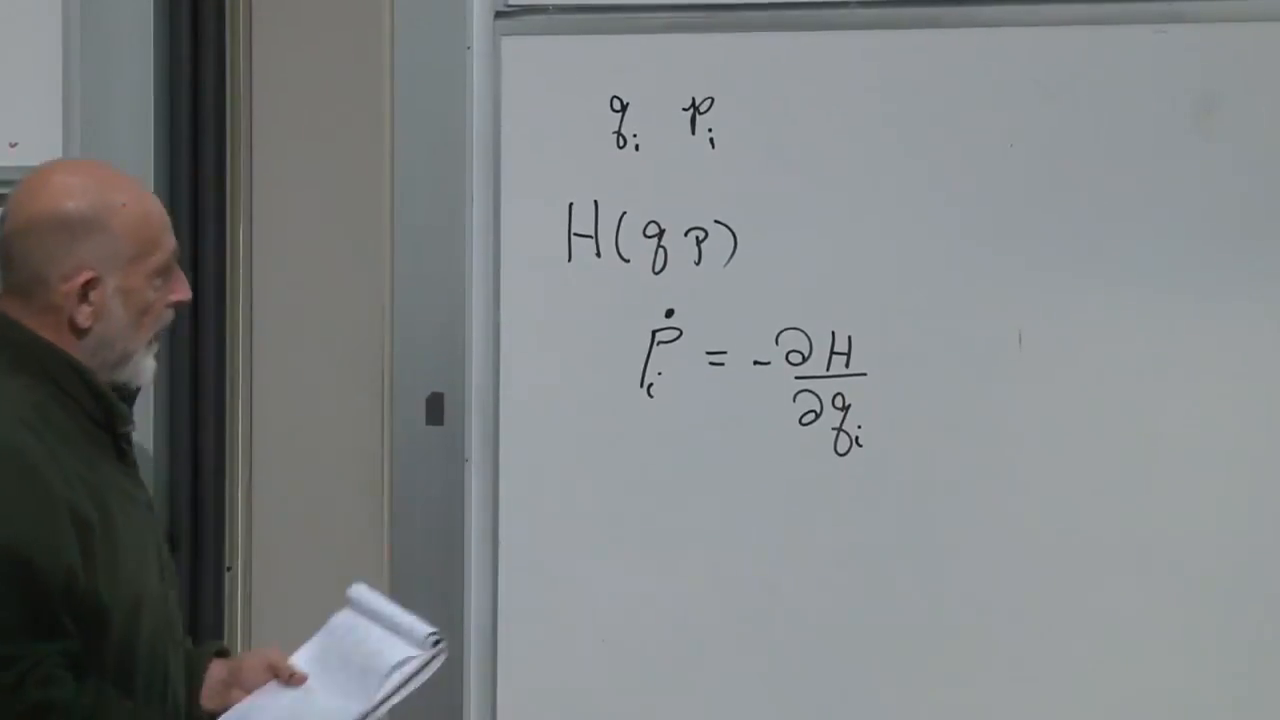
\includegraphics[width=0.82\textwidth]{lecture_07_figure_02.png}
  \caption{正則變數、函數\(H(q,p)\)，以及回顧一開始所列的動量側哈密頓方程。}
  \lectureframe{00:07:29}
\end{figure}

雖然方程以成對的指標形式出現，動力學不一定會逐對分離。哈密頓量可能耦合所有的\(q_i\)和\(p_i\)，因此，例如\(\dot p_1\)可能取決於整個系統的狀態。

\begin{classroomqa}
  \audiencequestion{這種表述現在是公理化的嗎？\(p\)和\(q\)之間假設了什麼關係？
  \lecturetimestamp{00:17:08--00:18:18}}
  \lecturerresponse{指定\(H(q,p)\)和正則變數對之後，哈密頓方程就定義了形式理論。並沒有普遍適用的額外假設\(p=m\dot q\)。對於動能為二次形式的普通笛卡兒粒子，這個關係成立；但採用其他座標或其他哈密頓量時，動量--速度關係也會不同。方程本身透過\(\dot q_i=\partial H/\partial p_i\)給出這個關係。至於提出的哈密頓量是否在自然界中實現，則是另一個物理問題。}
\end{classroomqa}

現在只需一步推理，就能得到能量守恆。沿著一條軌跡，\(H\)的全導數為
\begin{equation}
  \frac{dH}{dt}
  =
  \sum_i\left(
    \frac{\partial H}{\partial q_i}\dot q_i
    +\frac{\partial H}{\partial p_i}\dot p_i
  \right)
  +\frac{\partial H}{\partial t}.
  \label{eq:l7-total-h-derivative}
\end{equation}
最後一項表示\(q\)和\(p\)固定時仍存在的顯式時間依賴，例如外部指定的參數正在變化。代入式~\eqref{eq:l7-hamilton-equations}，
\begin{align}
  \frac{dH}{dt}
  &=
  \sum_i\left[
    \frac{\partial H}{\partial q_i}
    \frac{\partial H}{\partial p_i}
    -\frac{\partial H}{\partial p_i}
    \frac{\partial H}{\partial q_i}
  \right]
  +\frac{\partial H}{\partial t}\\
  &=\frac{\partial H}{\partial t}.
  \label{eq:l7-h-energy-rate}
\end{align}
總和中的每一項都會和配對項相消。因此，
\begin{equation}
  \frac{\partial H}{\partial t}=0
  \quad\Longrightarrow\quad
  \frac{dH}{dt}=0.
  \label{eq:l7-energy-conservation}
\end{equation}
對於封閉且具有時間平移不變性的系統，哈密頓量守恆，而且就是能量。

\begin{classroomqa}
  \audiencequestion{如果哈密頓量顯式依賴時間，會有什麼變化？\lecturetimestamp{00:10:32--00:12:33}}
  \lecturerresponse{式~\eqref{eq:l7-h-energy-rate}仍然成立，但子系統的能量不一定保持定值。顯式時間依賴通常表示有一個未納入模型的驅動源正在與系統交換能量。如果將這個驅動源納入更大的封閉系統，使它也成為動力學的一部分，那麼較大系統的哈密頓量便可再次不隨時間改變，總能量也會守恆。}
\end{classroomqa}

\section{相空間中的能量幾何}

現在假設\(H\)沒有顯式時間依賴。初始條件決定一個數值\(E\)，而相點會一直留在
\begin{equation}
  H(q,p)=E.
  \label{eq:l7-energy-surface}
\end{equation}
相空間有\(2n\)維。在正則點上，一個座標方程會定義一個\((2n-1)\)維超曲面。不同的\(E\)值會給出不同的超曲面。這些超曲面不一定封閉或緊緻；能量守恆只表示，從其中一個超曲面出發的軌跡永遠不會離開它。

對於前一講中經過適當縮放的諧振子，
\begin{equation}
  H=\frac{\omega}{2}(p^2+q^2).
  \label{eq:l7-oscillator-hamiltonian}
\end{equation}
因此，每個等能集合都是一個圓，
\begin{equation}
  p^2+q^2=\frac{2E}{\omega}.
  \label{eq:l7-oscillator-circle}
\end{equation}

\begin{figure}[htbp]
  \centering
  \includegraphics[width=0.84\textwidth]{lecture_07_figure_04.png}
  \caption{\(2n\)維相空間示意圖，以及用來引入等能面的諧振子哈密頓量。}
  \lectureframe{00:15:20}
\end{figure}

運動方程
\begin{equation}
  \dot q=\omega p,\qquad \dot p=-\omega q,
  \label{eq:l7-oscillator-flow}
\end{equation}
使相點沿著圓順時針運動。能量方程指出運動所在的曲線；哈密頓方程則給出沿著該曲線運動的方向和速率。

\begin{figure}[htbp]
  \centering
  \begin{tikzpicture}[scale=0.95]
    \draw[->] (-2.7,0) -- (2.7,0) node[right] {\(q\)};
    \draw[->] (0,-2.7) -- (0,2.7) node[above] {\(p\)};
    \draw[thick] (0,0) circle (0.8);
    \draw[thick] (0,0) circle (1.5);
    \draw[thick] (0,0) circle (2.2);
    \draw[->,very thick] (0,2.2) arc[start angle=90,end angle=40,radius=2.2];
    \draw[->,very thick] (1.5,0) arc[start angle=0,end angle=-50,radius=1.5];
    \draw[->,very thick] (0,-0.8) arc[start angle=-90,end angle=-140,radius=0.8];
  \end{tikzpicture}
  \caption{等能條件決定這些圓；振子方程則給出順時針的切向流。}
\end{figure}

\begin{classroomqa}
  \audiencequestion{哈密頓的兩個方程和\(H=E\)，是同一個方程的不同形式嗎？
  \lecturetimestamp{00:15:53--00:17:06}}
  \lecturerresponse{不是。哈密頓方程是描述一組正則變數對的兩條一階運動定律。它們蘊含\(dH/dt=0\)，由此可推出\(H=E\)。\(E\)的值由初始條件決定。方程\(H=E\)指出一個曲面，但本身不會指定沿著該曲面的速度。}
\end{classroomqa}

\section{從單一狀態到狀態流}

與其追蹤一個初始條件，不如讓相空間布滿所有可能的初始條件，再啟動時鐘。每個點代表一個完整的可能狀態，而每個狀態都依照哈密頓方程演化。我們可以把這些點想像成塵埃或假想流體。沒有任何物質真的被倒進相空間；流體只是讓我們能同時觀察所有軌跡的一種想像方式。

相空間中的速度場為
\begin{equation}
  \mathbf V(q,p,t)
  =
  (\dot q_1,\ldots,\dot q_n,\dot p_1,\ldots,\dot p_n).
  \label{eq:l7-phase-velocity}
\end{equation}
對於一組正則變數，我們寫成
\begin{equation}
  V_q=\dot q=\frac{\partial H}{\partial p},
  \qquad
  V_p=\dot p=-\frac{\partial H}{\partial q}.
  \label{eq:l7-phase-components}
\end{equation}
在每一點，哈密頓量都指定一個向量，表示相點接下來的運動方向。如果\(H\)不隨時間變化，向量場就是定常的：回到同一個相點時，速度仍相同。如果\(H\)依賴時間，向量場本身會隨時間改變，但在每一瞬間仍有明確定義。

\begin{figure}[htbp]
  \centering
  \includegraphics[width=0.84\textwidth]{lecture_07_figure_05.png}
  \caption{諧振子的速度場。向量沿圓的切線方向，且越接近原點，向量越短。}
  \lectureframe{00:24:50}
\end{figure}

對諧振子而言，每個半徑都以角速度\(\omega\)轉動。靠近原點的點，其線速度較小，因為它們在相同週期內走過的圓周較短。因此，整團塵埃會像剛體旋轉般轉動。

\begin{classroomqa}
  \audiencequestion{剛體般旋轉是否表示所有諧振子軌跡的週期都相同？\lecturetimestamp{00:21:10--00:21:42}}
  \lecturerresponse{是。週期與振幅無關，正是諧振子的特有性質。每個圓都以相同的角頻率\(\omega\)繞行，儘管較小圓上的相空間速度量值較小。}
\end{classroomqa}

\begin{classroomqa}
  \audiencequestion{相空間速度在每一點都相同嗎？
  \lecturetimestamp{00:24:29--00:25:37}}
  \lecturerresponse{不是。速度的方向和量值通常都會隨位置改變。對諧振子而言，向量沿著當地圓的切線方向，量值為\(\omega\sqrt{p^2+q^2}\)。所謂向量場，是指每一點各有一個向量，而不是把同一個向量複製到每個位置。}
\end{classroomqa}

\begin{classroomqa}
  \audiencequestion{這種假想流體中的粒子和密度，究竟代表什麼？\lecturetimestamp{00:56:03--00:58:40}}
  \lecturerresponse{每一個點代表整個力學系統的一個完整狀態，並非一個物理粒子。五個粒子在一維空間中運動，需要五個位置和五個動量，因此相空間有十個維度；若是在三維空間中，則需要三十個維度。這團塵埃代表一組彼此替代的可能狀態。如果流體圖像令人分心，只要取一個初始條件區域，讓其中每一點演化，再比較演化前後的相空間體積即可。}
\end{classroomqa}

\section{壓縮與散度}

要判斷這種假想流體是否會失去體積，先從一維開始。設直線上的點以速度\(v(x)\)運動。兩個相距\(\delta x\)的鄰近點，其速度差為
\begin{equation}
  \delta v \simeq \frac{dv}{dx}\,\delta x.
  \label{eq:l7-one-dimensional-strain}
\end{equation}
若\(dv/dx>0\)，前方的點移動得較快，兩點間隔便會拉長。若\(dv/dx<0\)，間隔便會壓縮。因此，定常的一維不可壓縮流必須滿足
\begin{equation}
  \frac{dv}{dx}=0.
  \label{eq:l7-one-dimensional-incompressible}
\end{equation}

\begin{figure}[htbp]
  \centering
  \includegraphics[width=0.84\textwidth]{lecture_07_figure_06.png}
  \caption{一維推導：\(dv/dx\)是局部拉伸或壓縮的速率。}
  \lectureframe{00:30:20}
\end{figure}

有兩種等價的觀點。我們可以跟著一段流體移動，觀察它的長度是否改變；也可以固定一個小區間，觀察單位時間內流入的量是否等於流出的量。前者跟著流體走，後者觀察流體經過。

在多維空間中，一個區域可以沿某個軸拉伸，同時沿另一個軸壓縮，而總體積仍不變。對於速度場\(\mathbf V=(V_x,V_y,V_z)\)，相關的局部速率是散度：
\begin{equation}
  \nabla\cdot\mathbf V
  =
  \frac{\partial V_x}{\partial x}
  +\frac{\partial V_y}{\partial y}
  +\frac{\partial V_z}{\partial z}.
  \label{eq:l7-spatial-divergence}
\end{equation}
散度為正表示局部膨脹，散度為負表示局部收縮；不可壓縮條件則是
\begin{equation}
  \nabla\cdot\mathbf V=0.
  \label{eq:l7-zero-divergence}
\end{equation}
固定小盒的流入量等於流出量，與隨流動移動的小盒體積保持不變，是同一個局部陳述。

\begin{figure}[htbp]
  \centering
  \includegraphics[width=0.86\textwidth]{lecture_07_figure_07.png}
  \caption{二維小盒、流速分量，以及定義散度的同座標偏導數之和。}
  \lectureframe{00:35:30}
\end{figure}

\begin{classroomqa}
  \audiencequestion{我們談的是普通空間中的流體，還是相空間中的流？ \lecturetimestamp{00:34:27--00:34:40}}
  \lecturerresponse{散度的推導首先是一般的流體力學論證。我們會將它應用於偶數維的相空間；其中的座標方向是\(q_i\)和\(p_i\)，速度分量則是\(\dot q_i\)和\(\dot p_i\)。}
\end{classroomqa}

現在回到離散狀態映射。在可逆循環中，每個節點都有一個箭頭進入，也有一個箭頭離開；一組選定的狀態在演化後仍包含相同數量的狀態。在匯中，進入的箭頭很多，離開的箭頭卻太少；幾種不同的可能狀態因此變得無法區分。

\begin{figure}[htbp]
  \centering
  \includegraphics[width=0.80\textwidth]{lecture_07_figure_08.png}
  \caption{離散匯的示意圖，用來重新連結散度與第一講中檢驗定律可逆性的方式。}
  \lectureframe{00:40:15}
\end{figure}

現在可以精確地提出連續情況下的問題：哈密頓流的散度是否為零，因此一小塊可區分狀態的區域不會被壓縮成更小的相空間體積？

\section{劉維爾定理}

\begin{theorem}[Liouville's theorem]對於光滑的哈密頓系統，正則相空間中的速度場散度為零：
\begin{equation}
  \sum_i\left(
    \frac{\partial\dot q_i}{\partial q_i}
    +\frac{\partial\dot p_i}{\partial p_i}
  \right)=0.
  \label{eq:l7-liouville-divergence}
\end{equation}
等價地說，哈密頓演化會保持正則相空間體積\(dq_1\cdots dq_n\,dp_1\cdots dp_n\)。
\end{theorem}

\begin{classroomqa}
  \audiencequestion{稱為\(V\)的分量，就是\(p\)點和\(q\)點嗎？\lecturetimestamp{00:42:20--00:43:22}}
  \lecturerresponse{是。對於一組正則變數，
  \(V_q=\dot q\)和\(V_p=\dot p\)。將所有這類導數依序排列，就得到完整相空間中流動的速度向量。}
\end{classroomqa}

對於一組正則變數，哈密頓方程給出
\begin{equation}
  V_p=-\frac{\partial H}{\partial q},
  \qquad
  V_q=\frac{\partial H}{\partial p}.
  \label{eq:l7-liouville-components}
\end{equation}
因此散度為
\begin{align}
  \frac{\partial V_p}{\partial p}
  +\frac{\partial V_q}{\partial q}
  &=
  -\frac{\partial}{\partial p}
    \left(\frac{\partial H}{\partial q}\right)
  +\frac{\partial}{\partial q}
    \left(\frac{\partial H}{\partial p}\right)\\
  &=
  -\frac{\partial^2H}{\partial p\,\partial q}
  +\frac{\partial^2H}{\partial q\,\partial p}
  =0.
  \label{eq:l7-liouville-proof}
\end{align}

\begin{figure}[htbp]
  \centering
  \includegraphics[width=0.86\textwidth]{lecture_07_figure_09.png}
  \caption{有限差分矩形示意圖，用來說明光滑函數的混合偏導數為何可以交換次序。}
  \lectureframe{00:47:30}
\end{figure}

取\(A,B,C,D\)這四個點，分別位於\(q\)-\(p\)平面上一個小矩形的四個角，就能看出混合偏導數相等。先對\(q\)取差分，再對\(p\)取差分，除去兩條小邊的長度後，得到
\begin{equation}
  F(B)+F(D)-F(A)-F(C).
  \label{eq:l7-finite-difference-combination}
\end{equation}
若以相反次序取差分，也會得到相同的組合。在小矩形極限下，只要所需的導數連續，便有
\(\partial_p\partial_qF=\partial_q\partial_pF\)。

\begin{figure}[htbp]
  \centering
  \includegraphics[width=0.88\textwidth]{lecture_07_figure_10.png}
  \caption{哈密頓方程將正則散度化為兩個符號相反的混合偏導數。}
  \lectureframe{00:50:20}
\end{figure}

對於多個自由度，每一組正則變數都會發生相同的相消：
\begin{align}
  \sum_i\left(
    \frac{\partial\dot p_i}{\partial p_i}
    +\frac{\partial\dot q_i}{\partial q_i}
  \right)
  &=
  \sum_i\left(
    -\frac{\partial^2H}{\partial p_i\,\partial q_i}
    +\frac{\partial^2H}{\partial q_i\,\partial p_i}
  \right)\\
  &=0.
  \label{eq:l7-many-pair-proof}
\end{align}
沿一個正則方向的拉伸，會由其共軛方向的壓縮抵銷。這種逐對相消具有更深的結構，並非彼此無關的座標軸之間偶然相消。

\begin{classroomqa}
  \audiencequestion{這裡是否省略了對所有正則變數對求和？
  \lecturetimestamp{00:52:00--00:52:36}}
  \lecturerresponse{是。式~\eqref{eq:l7-many-pair-proof}是對\(i\)求和，而且每一組\(q_i,p_i\)變數對中的兩個混合偏導數都各自相消。}
\end{classroomqa}

\begin{classroomqa}
  \audiencequestion{寫出的散度看起來是笛卡兒座標形式。換了座標之後，定理還成立嗎？
  \lecturetimestamp{00:52:50--00:53:22,\allowbreak\ 00:58:18--00:58:40}}
  \lecturerresponse{自然的表述採用正則座標和正則體積元素\(dq_1\cdots dq_n\,dp_1\cdots dp_n\)。正則變換又稱辛變換，它會同時改變座標與動量，並保持這個體積。在任意非正則座標中，體積測度必須包含雅可比因子；座標增量的直接乘積不一定是不變量。}
\end{classroomqa}

\begin{classroomqa}
  \audiencequestion{劉維爾定理是否要求哈密頓量不隨時間變化？\lecturetimestamp{00:53:43--00:55:51}}
  \lecturerresponse{不要求。能量守恆需要\(\partial H/\partial t=0\)，但散度的推導只在固定時間下對\(q_i\)和\(p_i\)微分。對於\(H(q,p,t)\)，混合偏導數仍然會相消。因此，含時哈密頓量會產生隨時間變化、但每一瞬間都保持體積的正則流。}
\end{classroomqa}

\section{體積保持意味著什麼，又不意味著什麼}

取一個初始條件的小區域\(R_0\)，讓其中每個點演化時間\(t\)。劉維爾定理指出
\begin{equation}
  \operatorname{Vol}(R_t)=\operatorname{Vol}(R_0).
  \label{eq:l7-volume-preservation}
\end{equation}
這個區域可能移動、旋轉、剪切，並拉伸成細長的絲狀結構。受到保護的是體積，而不是形狀。在有限時間的光滑哈密頓演化中，不同的相點不會合併。

在有限時間內，光滑的哈密頓流是可逆映射；其光滑逆映射可藉由反向演化得到。這也說明了課堂上的說法：一團連通區域不會被掐斷成不連通的部分。流會連續地形變這個區域並保持其拓撲；不過，極細的連接頸部可能讓兩個瓣在有限解析度下看起來像是分開的。

\begin{figure}[htbp]
  \centering
  \includegraphics[width=0.86\textwidth]{lecture_07_figure_12.png}
  \caption{相空間區域可能發生的形變。光滑的哈密頓流可以形成細長的頸部，但不會在有限時間內真正斷裂成各自獨立演化的部分。}
  \lectureframe{01:04:55}
\end{figure}

\begin{classroomqa}
  \audiencequestion{相空間中的一個區域能否被掐斷，分裂成兩部分？\lecturetimestamp{01:04:10--01:05:49}}
  \lecturerresponse{在有限時間的光滑確定性哈密頓流下不會。即使在假想的掐斷點上，那仍是一個相點，只對應一個指定速度，而不會有兩個互不相容的方向。這個區域可以形成非常長而狹窄的連接細絲，但演化仍是一對一的，不會把它撕裂。}
\end{classroomqa}

\begin{classroomqa}
  \audiencequestion{被拉伸的區域中，兩個相距很遠的瓣在物理上仍相連嗎？它們是否量子糾纏？
  \lecturetimestamp{01:08:01--01:09:16}}
  \lecturerresponse{這並不表示它們在物理上相連。這個區域代表一組可能的初始條件，而不是一個物質物體。稱它為同一個區域，只是表示這些狀態源自同一個集合；這並不表示它們彼此間存在作用力或量子糾纏。}
\end{classroomqa}

\begin{classroomqa}
  \audiencequestion{剛性擺在鉛直向上的不穩定平衡附近會發生什麼事？順時針和逆時針的軌跡會重疊嗎？
  \lecturetimestamp{01:07:07--01:07:47}}
  \lecturerresponse{鄰近的初始條件可能分別沿著差異極大的軌跡演化，形成前面提到的細絲。它們不會變成同一個相點：無窮小位移或動量的正負號，會區分平衡點的兩側。完全平衡的狀態則有唯一確定的運動；在理想模型中，它會保持在平衡位置。}
\end{classroomqa}

\subsection{位置空間膨脹與動量空間收縮}

如果一個正則變換將位置範圍放大\(a\)倍，則共軛動量的尺度會以其倒數縮小：
\begin{equation}
  q\longrightarrow aq,
  \qquad
  p\longrightarrow \frac{p}{a},
  \qquad
  dq\,dp\longrightarrow dq\,dp.
  \label{eq:l7-canonical-scaling}
\end{equation}
這正是氣體膨脹例子中清楚的相空間意涵。在絕熱膨脹中，可及的普通空間區域增大，典型動量則下降，氣體因而冷卻。詳細的熱力學關係取決於維度、膨脹過程和交互作用；劉維爾定理提供的是體積限制，而不是所有熱力學係數。

\begin{classroomqa}
  \audiencequestion{同樣的推理是否也適用於宇宙膨脹，即使是突然膨脹也一樣嗎？\lecturetimestamp{00:53:23--00:56:00}}
  \lecturerresponse{只要完整的動力學是哈密頓形式，劉維爾定理就適用，包括顯含時間的正則變數。位置方向的膨脹必須伴隨正則動量方向相應的收縮。不過，宇宙學中的尺度因子、受控的氣體膨脹，以及自由爆炸的雲，並非同一種物理過程。距離與退行速度之間類似哈勃定律的關聯，可能是因為速度較快的物體移動得更遠；絕熱冷卻所涉及的則是局部動量分佈的收縮。無論是哪種情況，定理限制的都是完整的相空間映射。}
\end{classroomqa}

\begin{classroomqa}
  \audiencequestion{劉維爾定理有什麼實際用途？
  \lecturetimestamp{01:06:16--01:07:04}}
  \lecturerresponse{它是統計力學的核心定理，能描述微觀狀態系綜如何演化，也是相空間體積與熵之間關係的基礎。氣體膨脹與冷卻是直接的例子；往後它也會成為分析平衡與非平衡現象的基本工具。}
\end{classroomqa}

\section{形狀劇烈改變的流}

諧振子的流是剛體旋轉，因此既保持面積，也保持形狀。這是特殊情況。為了看出體積保持和剛體性質的差異，考慮
\begin{equation}
  H=\lambda pq,
  \label{eq:l7-pq-hamiltonian}
\end{equation}
其中\(\lambda\)的單位是時間的倒數。課堂上取\(\lambda=1\)；保留這個參數可讓量綱一目了然。

\begin{figure}[htbp]
  \centering
  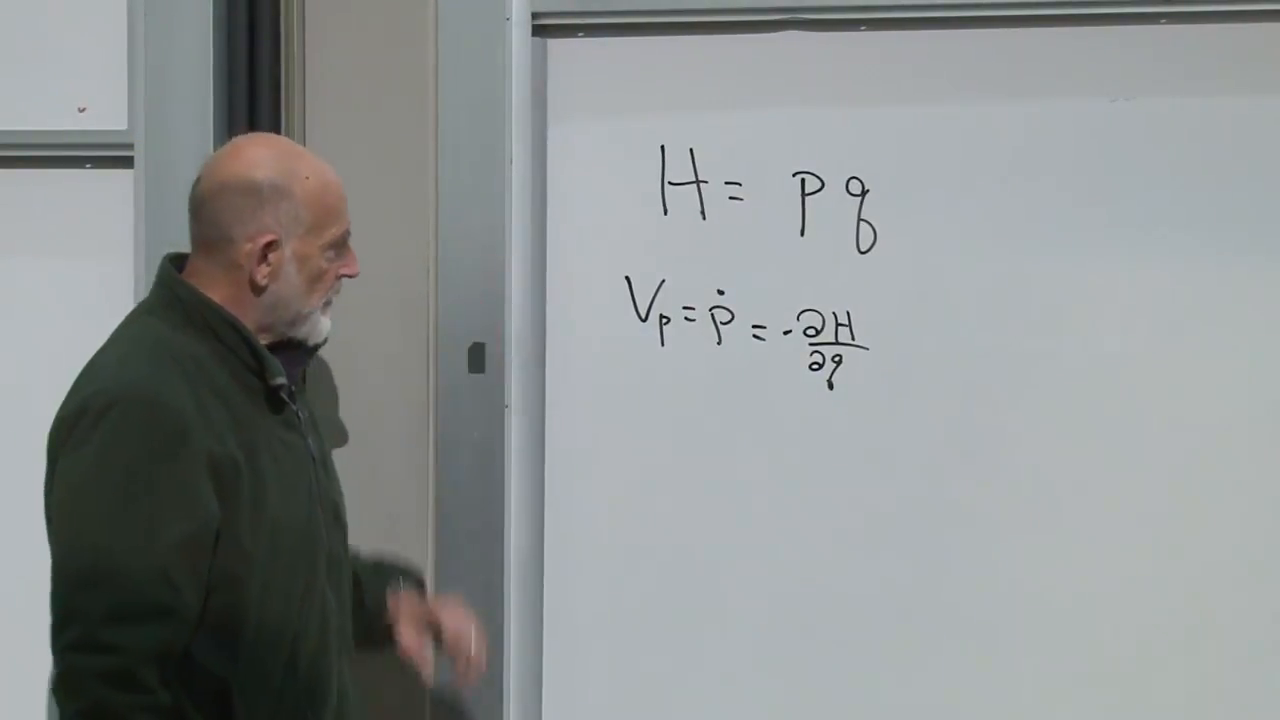
\includegraphics[width=0.82\textwidth]{lecture_07_figure_03.png}
  \caption{\(H=pq\)例子的開頭，以及第一個相空間速度分量。}
  \lectureframe{01:00:11}
\end{figure}

哈密頓方程為
\begin{equation}
  \dot p=-\lambda p,
  \qquad
  \dot q=\lambda q,
  \label{eq:l7-pq-flow}
\end{equation}
其解為
\begin{equation}
  p(t)=p_0e^{-\lambda t},
  \qquad
  q(t)=q_0e^{\lambda t}.
  \label{eq:l7-pq-solutions}
\end{equation}
一個正方形小區域在\(p\)方向上以指數方式縮小，同時在\(q\)方向上以相同因子拉長：
\begin{equation}
  \Delta p(t)\Delta q(t)
  =
  \Delta p(0)\Delta q(0).
  \label{eq:l7-pq-area}
\end{equation}
從局部散度也能驗證這個結果：
\begin{equation}
  \frac{\partial\dot p}{\partial p}
  +\frac{\partial\dot q}{\partial q}
  =-\lambda+\lambda=0.
  \label{eq:l7-pq-divergence}
\end{equation}

\begin{figure}[htbp]
  \centering
  \includegraphics[width=0.86\textwidth]{lecture_07_figure_11.png}
  \caption{在\(H=pq\)流作用下，一個緊緻的小區域被拉長成細長條帶，同時保持面積。}
  \lectureframe{01:02:10}
\end{figure}

\begin{classroomqa}
  \audiencequestion{既然\(pq\)的單位是作用量，劉維爾定理是否表示作用量守恆？\lecturetimestamp{01:03:00--01:04:09}}
  \lecturerresponse{不是。這個定理守恆的是相空間體積。對一組正則變數而言，\(dq\,dp\)的單位是作用量；這個量綱特徵也預示了量子力學，因為相空間胞元的測量單位由\(\hbar\)決定。但乘積\(pq\)本身不是哈密頓作用量泛函，也不會只因量綱相同就自動成為角動量。}
\end{classroomqa}

這個例子也顯示角度不一定保持不變。在式~\eqref{eq:l7-pq-solutions}所示的縮放下，兩臂縮放不等的直角十字，其度量形狀會受到剪切，但面積仍保持不變。劉維爾定理是面積或體積守恆定理，不是一般歐幾里得剛體變換定理。

\section{阻尼會產生匯}

為了看出這個定理排除了什麼，考慮阻尼振子的約化方程：
\begin{equation}
  m\ddot x=-kx-c\dot x,
  \qquad c>0.
  \label{eq:l7-damped-newton}
\end{equation}
令\(p=m\dot x\)。則
\begin{equation}
  \dot x=\frac{p}{m},
  \qquad
  \dot p=-kx-\frac{c}{m}p.
  \label{eq:l7-damped-first-order}
\end{equation}
沒有阻尼時，相點會繞著原點作圓周運動。有阻尼時，能量會傳給周圍介質的微觀自由度，軌道則向內螺旋。

\begin{figure}[htbp]
  \centering
  \includegraphics[width=0.84\textwidth]{lecture_07_figure_13.png}
  \caption{阻尼振子方程，以及它在\(x\)-\(p\)平面上的向內螺旋軌跡。}
  \lectureframe{01:13:30}
\end{figure}

這個二維約化流的散度為
\begin{equation}
  \frac{\partial\dot x}{\partial x}
  +\frac{\partial\dot p}{\partial p}
  =
  0-\frac{c}{m}<0.
  \label{eq:l7-damped-divergence}
\end{equation}
每一個有限區域都會收縮。原點是個匯，是離散狀態映射中多個箭頭匯入同一狀態的連續類比。

\begin{figure}[htbp]
  \centering
  \includegraphics[width=0.88\textwidth]{lecture_07_figure_14.png}
  \caption{阻尼相空間中的速度分量，用來導出負散度\(-c/m\)。}
  \lectureframe{01:16:05}
\end{figure}

這並不表示微觀力學違反劉維爾定理。兩個變數\(x,p\)沒有包含數量龐大的環境自由度，而振子的能量正是傳給了這些自由度。即使約化後的\(x,p\)描述呈現收縮，振子與環境合成的較大系統仍可能遵循哈密頓動力學並保持體積。

\begin{classroomqa}
  \audiencequestion{儘管阻尼振子在這個約化相空間中不是哈密頓系統，它仍然由牛頓方程描述嗎？
  \lecturetimestamp{01:20:09--01:21:12}}
  \lecturerresponse{是的。牛頓第二定律\(F=ma\)可以納入根據經驗給定的阻力。初等的拉格朗日描述\(L=T-V\)和哈密頓描述直接適用於保守力；更一般的拉格朗日量也能處理某些依賴速度的力。然而，對孤立的一對\(x,p\)而言，馬可夫型摩擦項描述的是約化後的耗散動力學，而不是封閉的正則哈密頓系統。}
\end{classroomqa}

\begin{classroomqa}
  \audiencequestion{如果阻尼方程能以無限精度反向積分，資訊真的會丟失嗎？
  \lecturetimestamp{01:25:16--01:27:17}}
  \lecturerresponse{在任何有限時間內，理想的微分方程仍有反函數，因此可以用精確資料反向演化。更精確地說，有限的相空間胞元會呈指數收縮。因此，要重建它們過去的狀態，就需要指數級提高精度；到了無限時間，所有軌跡都會趨近匯點。這是最接近離散「選項消失」圖像的連續經典類比，並不表示兩個精確解在有限時間內真的會合而為一。}
\end{classroomqa}

\begin{classroomqa}
  \audiencequestion{向量場能否散度為零，卻不是由哈密頓量導出的？\lecturetimestamp{01:18:21--01:22:34}}
  \lecturerresponse{當然可以。哈密頓形式是散度為零的充分條件，但不是必要條件。任意不可壓縮速度場都可能散度為零，卻不是同一空間上的正則哈密頓場。三維不可壓縮流體的速度場就是課堂上的例子：三個座標本身無法構成正則共軛對。完整的流體力學或許有更精細的無限維哈密頓表述，但這不會改變此處所說的單向蘊含關係。}
\end{classroomqa}

\section{問題進一步揭示的區別}

\begin{classroomqa}
  \audiencequestion{等能面上的運動，與整個相空間體積保持不變有何關係？
  \lecturetimestamp{01:28:47--01:30:41}}
  \lecturerresponse{兩者是哈密頓結構各自帶來的結果。如果\(H\)不顯含時間，每條軌跡都會留在各自的能量面上。一個有限區域可能跨越許多這樣的能量面；劉維爾定理則指出，整個區域的體積保持不變。對諧振子而言，這個區域的形狀也會保持不變，因為其流動是剛性旋轉。而\(H=pq\)的區域只保持面積，不保持形狀。}
\end{classroomqa}

\begin{classroomqa}
  \audiencequestion{機械功在哈密頓描述中扮演什麼角色？\lecturetimestamp{01:30:44--01:32:57}}
  \lecturerresponse{功描述能量如何穿越所選定的系統邊界。外部作用者可以舉起重物或改變參數，藉此改變子系統的能量；子系統獲得的能量，正是作用者失去的能量。如果把雙方都納入同一個封閉模型，焦點就回到總能量守恆，以及子系統之間的能量交換。}
\end{classroomqa}

\begin{classroomqa}
  \audiencequestion{體積保持不變，也代表拓撲和角度保持不變嗎？\lecturetimestamp{01:33:00--01:33:37}}
  \lecturerresponse{光滑的有限時間哈密頓流會保持拓撲，因為它是可逆的連續形變。但它通常不會保持歐幾里得角度或形狀。諧振子的剛性旋轉確實會保持角度和形狀，而\(H=pq\)的拉伸則說明了這為何只是特例。}
\end{classroomqa}

\begin{classroomqa}
  \audiencequestion{省略勒讓德變換，是因為它沒有物理意義嗎？\lecturetimestamp{01:33:43--01:34:48}}
  \lecturerresponse{不是。勒讓德變換很有用，它把速度描述轉換為動量描述，並在映射正則時導出\(H=\sum_i p_i\dot q_i-L\)。即使沒有特別強調正式名稱，這個構造也已經反覆用過；只是目前這個定理不需要完整的一般理論。}
\end{classroomqa}

\section{泊松括號：進一步的簡化}

最後幾分鐘回到歷史主題。十九世紀的力學一再尋找簡潔的結構，將表面上不同的系統連結起來---力學與幾何光學、粒子與光線、經典軌跡與波動描述。泊松括號也是這類結構之一，在量子力學中尤其重要。

令\(F(q,p)\)為相空間上的任意函數。它可以是座標、動量、乘積\(qp\)，或角動量。沿著運動，其時間變化率為\begin{equation}
  \frac{dF}{dt}
  =
  \sum_i\left(
    \frac{\partial F}{\partial q_i}\dot q_i
    +\frac{\partial F}{\partial p_i}\dot p_i
  \right).
  \label{eq:l7-f-time-derivative}
\end{equation}
代入哈密頓方程：
\begin{equation}
  \frac{dF}{dt}
  =
  \sum_i\left(
    \frac{\partial F}{\partial q_i}
    \frac{\partial H}{\partial p_i}
    -
    \frac{\partial F}{\partial p_i}
    \frac{\partial H}{\partial q_i}
  \right).
  \label{eq:l7-f-hamiltonian-derivative}
\end{equation}

\begin{figure}[htbp]
  \centering
  \includegraphics[width=0.88\textwidth]{lecture_07_figure_15.png}
  \caption{一般相空間函數\(F(q,p)\)的時間導數所遵循的鏈鎖律。}
  \lectureframe{01:42:40}
\end{figure}

這個反覆出現的反對稱組合值得有個名稱。對任意兩個函數\(F\)和\(G\)，將它們的泊松括號定義為
\begin{equation}
  \boxed{
  \{F,G\}
  =
  \sum_i\left(
    \frac{\partial F}{\partial q_i}
    \frac{\partial G}{\partial p_i}
    -
    \frac{\partial F}{\partial p_i}
    \frac{\partial G}{\partial q_i}
  \right).}
  \label{eq:l7-poisson-bracket}
\end{equation}

\begin{figure}[htbp]
  \centering
  \includegraphics[width=0.86\textwidth]{lecture_07_figure_16.png}
  \caption{由兩個函數的導數構成的組合，提升為泊松括號。}
  \lectureframe{01:44:15}
\end{figure}

式~\eqref{eq:l7-f-hamiltonian-derivative}可改寫為
\begin{equation}
  \boxed{\frac{dF}{dt}=\{F,H\}.}
  \label{eq:l7-hamiltonian-poisson-evolution}
\end{equation}
如果\(F\)還顯含時間，則再加上\(\partial F/\partial t\)。令\(F=q_i\)或\(F=p_i\)，即可得到哈密頓的兩個方程，因此式~\eqref{eq:l7-hamiltonian-poisson-evolution}以簡潔形式表達了完整的動力學。

記號總是可以人為地簡化---例如，可以把許多方程各自平方後相加，再稱所得結果為一個方程。這麼做只會隱藏結構，而非揭示結構。泊松括號之所以有用，恰恰是因為它的代數能整理時間演化、守恆量與對稱性。下一步要發展這套代數，再將它用於角動量；角動量的結構在經典力學與量子理論中都至關重要。

\section{可逆性的連續意義}

現在可以完整陳述這一連串想法。當哈密頓量不顯含時間時，哈密頓方程會使\(H\)保持不變，因此每條軌跡都留在等能超曲面上。同一組方程也為相空間中的每一點指定一個速度。由於混合偏導數會兩兩抵消，這個速度場的散度為零。因此，一整個可能狀態區域的正則體積會保持不變。

這就是「一條軌跡進入、一條軌跡離開」的連續版本。形狀和角度都可能改變，相鄰軌跡也可能大幅分離。在光滑且封閉的哈密頓描述中，不可能發生的是：將有限的一組可能狀態壓縮到更小的相空間體積。\(H=pq\)流展示了系統可以拉伸；約化後的阻尼振子則展示了一旦不再滿足哈密頓條件，就會出現匯點。接著，泊松括號將同一套動力學濃縮成一個陳述：哈密頓量生成所有時間導數。
\chapter{泊松括號、生成元與角動量}

\lectureoverview{泊松括號不只是簡潔改寫哈密頓方程的工具，也是一種能生成變換的代數運算。與哈密頓量取泊松括號會生成時間演化；與動量取括號會生成平移；與角動量取括號則會生成旋轉。用這種語言來說，對稱性與守恆是同一個零括號的兩種解讀。我們將從諧振子出發發展這個觀念，再利用角動量代數推導陀螺進動，全程不必引入尤拉角。}

\section{沿哈密頓軌跡變化的函數}

設
\[
  F=F(q_1,\ldots,q_n,p_1,\ldots,p_n)
\]
是相空間上的充分可微函數。可以從兩個角度來看它。首先，它為相空間中的每一點指定一個數值。其次，選定一條哈密頓軌跡後，由於點 \((q(t),p(t))\) 隨時間移動，這個函數也就成為時間的函數。沿著該軌跡，
\begin{equation}
  \frac{dF}{dt}
  =
  \sum_i\left(
    \frac{\partial F}{\partial q_i}\dot q_i
    +\frac{\partial F}{\partial p_i}\dot p_i
  \right).
  \label{eq:l8-chain-rule}
\end{equation}
哈密頓方程
\begin{equation}
  \dot q_i=\frac{\partial H}{\partial p_i},
  \qquad
  \dot p_i=-\frac{\partial H}{\partial q_i},
  \label{eq:l8-hamilton-equations}
\end{equation}
可將上式改寫為
\begin{equation}
  \frac{dF}{dt}
  =
  \sum_i\left(
    \frac{\partial F}{\partial q_i}
    \frac{\partial H}{\partial p_i}
    -
    \frac{\partial F}{\partial p_i}
    \frac{\partial H}{\partial q_i}
  \right).
  \label{eq:l8-fdot-expanded}
\end{equation}
右側這個組合在經典力學中屢屢出現，即使其中兩個函數都不是哈密頓量也是如此。因此我們定義
\begin{equation}
  \boxed{
  \{F,G\}
  =
  \sum_i\left(
    \frac{\partial F}{\partial q_i}
    \frac{\partial G}{\partial p_i}
    -
    \frac{\partial F}{\partial p_i}
    \frac{\partial G}{\partial q_i}
  \right).}
  \label{eq:l8-poisson-definition}
\end{equation}
所以，式 ~\eqref{eq:l8-fdot-expanded} 可寫成
\begin{equation}
  \boxed{\dot F=\{F,H\}.}
  \label{eq:l8-time-generator}
\end{equation}

\begin{classroomqa}
  \audiencequestion{若將第二個函數從 \(H\) 換成任意函數 \(G\)，這個括號仍會是 \(F\) 的時間導數嗎？
  \lecturetimestamp{00:05:45--00:06:15}}
  \lecturerresponse{不會。記號推廣時，聽眾注意到了一個重要之處：式 ~\eqref{eq:l8-poisson-definition} 對任意兩個相空間函數定義了 \(\{F,G\}\)，但
  \(\dot F=\{F,G\}\) 只有在 \(G\) 是哈密頓量時才成立。一般的 \(G\) 會生成不同的無窮小變換。}
\end{classroomqa}

將時間的微小變化寫成
\begin{equation}
  \delta_t F=\epsilon\,\{F,H\}.
  \label{eq:l8-small-time-step}
\end{equation}
很有用。這種寫法也預示了後續的內容：時間演化只是由泊松括號生成的一大類變換之一。

\section{括號的代數}

現在可以把括號當作一套獨立的演算來使用。它的規則可由普通微分推出：
\begin{align}
  \{A,B\}&=-\{B,A\}, \label{eq:l8-antisymmetry}\\
  \{A+B,C\}&=\{A,C\}+\{B,C\}, \label{eq:l8-additivity}\\
  \{\lambda A,B\}&=\lambda\{A,B\},
    \quad \lambda\ \text{constant}, \label{eq:l8-scalar-rule}\\
  \{AB,C\}&=A\{B,C\}+\{A,C\}B. \label{eq:l8-leibniz}
\end{align}
這四行依序表達反對稱性、可加性、對常數乘法的線性，以及萊布尼茲法則。經典相空間函數的乘法是可交換的，因此最後一行中的普通因子 \(A\) 與 \(B\) 放置次序無關緊要。量子力學中的算符則不再如此。反對稱性也表示
\begin{equation}
  \{A,A\}=0.
  \label{eq:l8-self-bracket}
\end{equation}

正則座標的基本括號為
\begin{equation}
  \boxed{
  \{q_i,q_j\}=0,\qquad
  \{p_i,p_j\}=0,\qquad
  \{q_i,p_j\}=\delta_{ij}.}
  \label{eq:l8-canonical-brackets}
\end{equation}
任何只依賴 \(q_i\) 的函數，與任何只依賴 \(q_i\) 的函數取括號都為零；只依賴 \(p_i\) 的函數也有類似性質。只有正則座標與其共軛動量相遇時，括號才可能不為零。式 ~\eqref{eq:l8-canonical-brackets} 中的克羅內克 {\proseunicodefont δ} 表示只有指標相同時才會相遇。

\subsection{以諧振子作為檢驗}

考慮
\begin{equation}
  H=\frac{p^2}{2m}+\frac{kq^2}{2}.
  \label{eq:l8-oscillator-hamiltonian}
\end{equation}
現在我們刻意只使用括號規則和式 ~\eqref{eq:l8-time-generator}。首先，
\begin{align}
  \dot q
  &=\{q,H\}\\
  &=\frac{1}{2m}\{q,p^2\}\\
  &=\frac{1}{2m}\left(p\{q,p\}+\{q,p\}p\right)\\
  &=\frac{p}{m}.
  \label{eq:l8-qdot-oscillator}
\end{align}
勢能項會消失，因為 \(\{q,q^2\}=0\)。同樣地，
\begin{align}
  \dot p
  &=\{p,H\}\\
  &=\frac{k}{2}\{p,q^2\}\\
  &=\frac{k}{2}\left(q\{p,q\}+\{p,q\}q\right)\\
  &=-kq.
  \label{eq:l8-pdot-oscillator}
\end{align}
這個負號正是反對稱性 \(\{p,q\}=-\{q,p\}=-1\) 所致。合併這兩個一階方程，得到
\begin{equation}
  m\ddot q=-kq.
  \label{eq:l8-hooke-equation}
\end{equation}

\begin{figure}[htbp]
  \centering
  
\includegraphics[width=0.82\textwidth]{lecture_08_figure_01.png}
  \caption{諧振子的哈密頓量，以及分別導出 \(\dot q=p/m\) 與 \(\dot p=-kq\) 的括號計算。}
  \lectureframe{00:23:20}
\end{figure}

計算過程中，全班試著找出一個表示 \emph{取泊松括號} 的動詞，暫時選定了 \emph{泊松化}。這個玩笑點出觀點上的真正轉變：掌握代數規則後，就能直接運用它，不必每次都從定義重新推導結果。

\begin{classroomqa}
  \audiencequestion{這種數學結構是群，還是代數？它有反元素嗎？\lecturetimestamp{00:23:48--00:24:16}}
  \lecturerresponse{它不是群：括號運算不具備群所需的單位元與反元素。相空間函數構成一個泊松代數：它們具有普通的交換乘法與加法，並配有滿足萊布尼茲法則的反對稱括號。還需要另一個恆等式，也就是雅可比恆等式，才能符合一般的抽象定義；本講不會進一步推導它。}
\end{classroomqa}

\begin{classroomqa}
  \audiencequestion{泊松括號與量子對易子有什麼關聯？\lecturetimestamp{00:24:18--00:25:00}}
  \lecturerresponse{本講只先略作介紹。過渡到量子力學時，經典括號在概略上會以
  \[
    \{A,B\}_{\mathrm{PB}}
    \longleftrightarrow
    \frac{1}{i\hbar}[\widehat A,\widehat B].
  \]
  取代。不過，這種對應關係須附帶算符排序與量子化方面的條件；這裡不會把它當作定理使用。}
\end{classroomqa}

對諧振子而言，泊松括號只是重新推導出哈密頓方程。當生成元是守恆量而非 \(H\) 時，這套方法真正的簡便之處才會顯現。

\section{從旋轉對稱性導出角動量}

回想本課程前面用過的諾特構造之無窮小形式。若連續對稱性使座標產生變化
\begin{equation}
  \delta q_i=\epsilon F_i(q),
  \label{eq:l8-noether-variation}
\end{equation}
那麼，在此處討論的情況下，相應的守恆量為
\begin{equation}
  G=\sum_i p_iF_i(q).
  \label{eq:l8-noether-charge}
\end{equation}
整體因子 \(\epsilon\) 可以省略：守恆量乘上一個固定數，不會改變守恆定律。

取一個粒子，讓它繞 \(z\) 軸作無窮小旋轉。按照本講採用的方向約定，
\begin{equation}
  \delta x=-\epsilon y,\qquad
  \delta y=\epsilon x,\qquad
  \delta z=0.
  \label{eq:l8-z-rotation}
\end{equation}
式 ~\eqref{eq:l8-noether-charge} 給出
\begin{equation}
  L_z=-p_xy+p_yx=xp_y-yp_x.
  \label{eq:l8-lz}
\end{equation}
循環置換 \(x\)、\(y\) 與 \(z\)，可得
\begin{equation}
  \boxed{\begin{aligned}
    L_x&=yp_z-zp_y,\\
    L_y&=zp_x-xp_z,\\
    L_z&=xp_y-yp_x.
  \end{aligned}}
  \label{eq:l8-angular-components}
\end{equation}
這些就是 \begin{equation}
  \boldsymbol L=\boldsymbol r\times\boldsymbol p.
  \label{eq:l8-cross-product}
\end{equation} 的分量。

\begin{figure}[htbp]
  \centering
  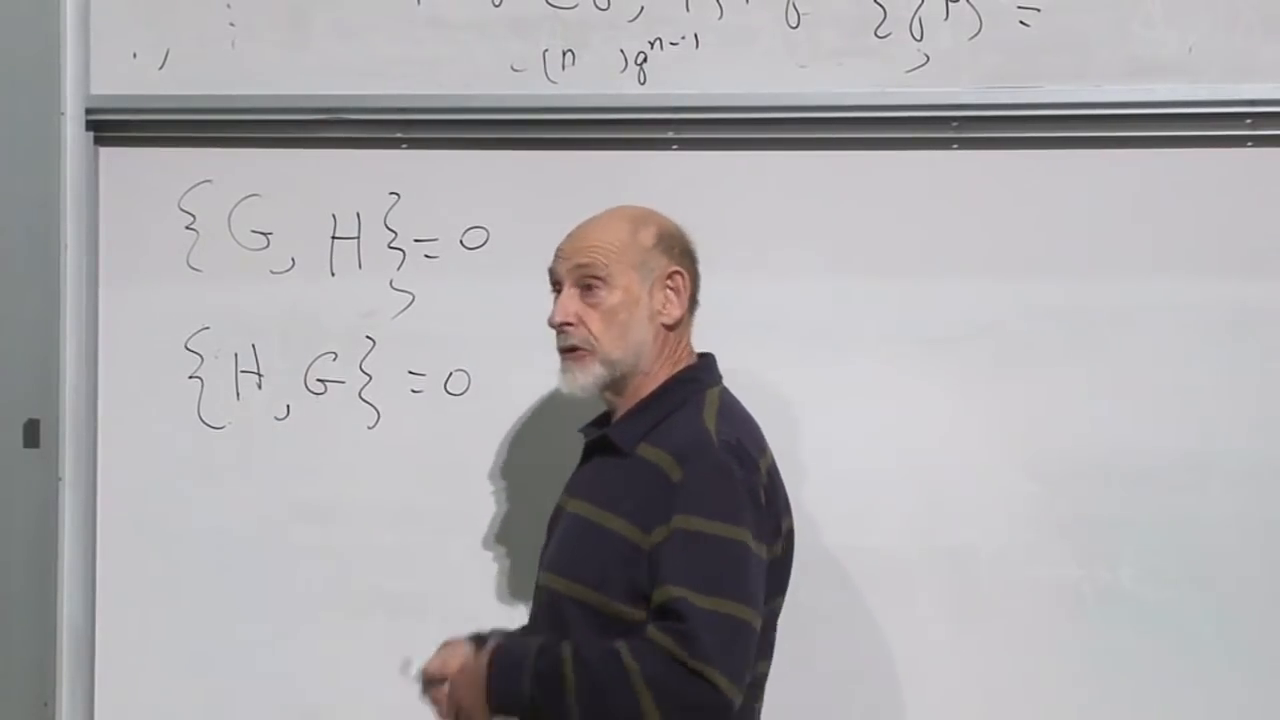
\includegraphics[width=0.82\textwidth]{lecture_08_figure_02.png}
  \caption{角動量的三個笛卡兒分量及其簡潔的叉積表示式。}
  \lectureframe{00:34:00}
\end{figure}

繞任意單位向量 \(\boldsymbol n\) 的旋轉，其生成元為
\begin{equation}
  L_{\boldsymbol n}=\boldsymbol n\cdot\boldsymbol L.
  \label{eq:l8-arbitrary-axis}
\end{equation}
對孤立且具旋轉不變性的系統，角動量的三個分量都守恆。若系統只在繞某一軸旋轉時仍具對稱性，則只有沿該軸的分量必定守恆。

\section{角動量生成旋轉}

我們先不急著求解旋轉動力學問題，而來看看 \(L_z\) 在取括號後會如何作用。利用式 ~\eqref{eq:l8-lz}，
\begin{align}
  \{x,L_z\}
  &=\{x,xp_y-yp_x\}
   =-y\{x,p_x\}
   =-y,\\
  \{y,L_z\}
  &=\{y,xp_y-yp_x\}
   =x\{y,p_y\}
   =x,\\
  \{z,L_z\}&=0.
  \label{eq:l8-position-rotation-brackets}
\end{align}
所得結果恰好就是式 ~\eqref{eq:l8-z-rotation} 中的係數。

\begin{figure}[htbp]
  \centering
  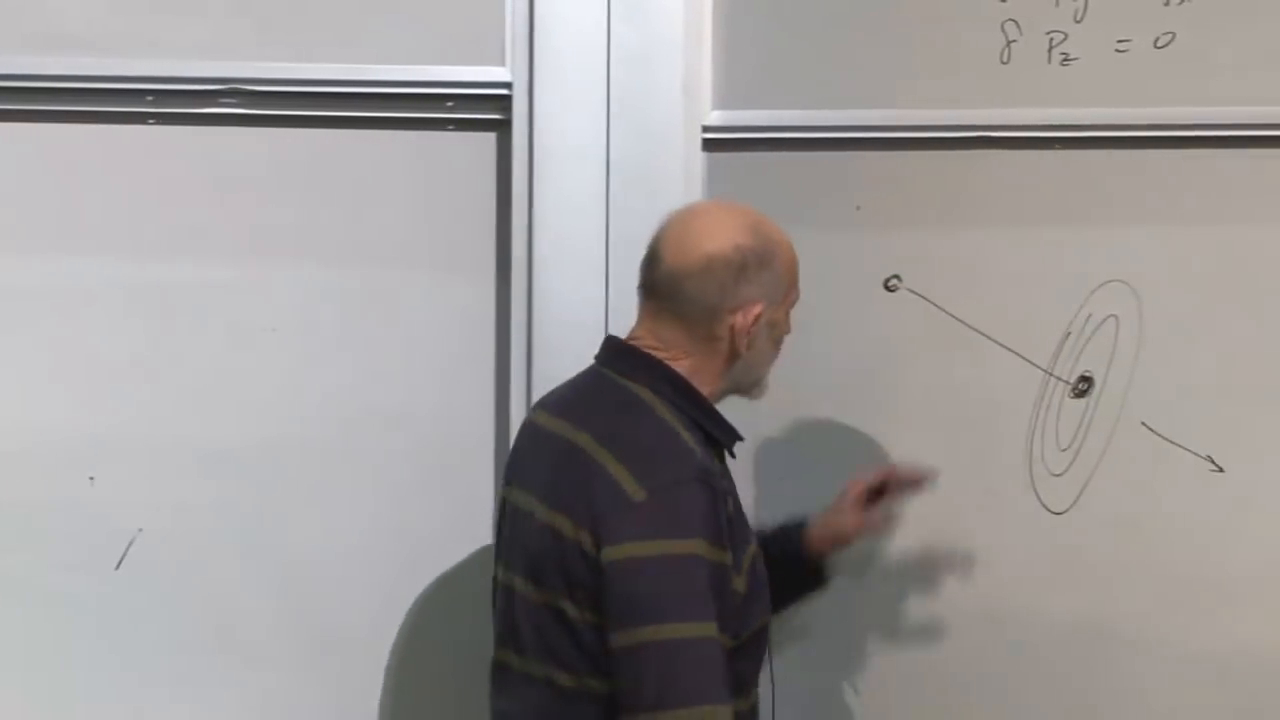
\includegraphics[width=0.82\textwidth]{lecture_08_figure_03.png}
  \caption{座標與 \(L_z\) 的括號：取括號會重現 \((x,y,z)\) 的無窮小旋轉。}
  \lectureframe{00:38:41}
\end{figure}

動量也是向量，同樣的計算得到
\begin{equation}
  \begin{aligned}
    \{p_x,L_z\}&=-p_y,\\
    \{p_y,L_z\}&=p_x,\\
    \{p_z,L_z\}&=0.
  \end{aligned}
  \label{eq:l8-momentum-rotation-brackets}
\end{equation}

\begin{figure}[htbp]
  \centering
  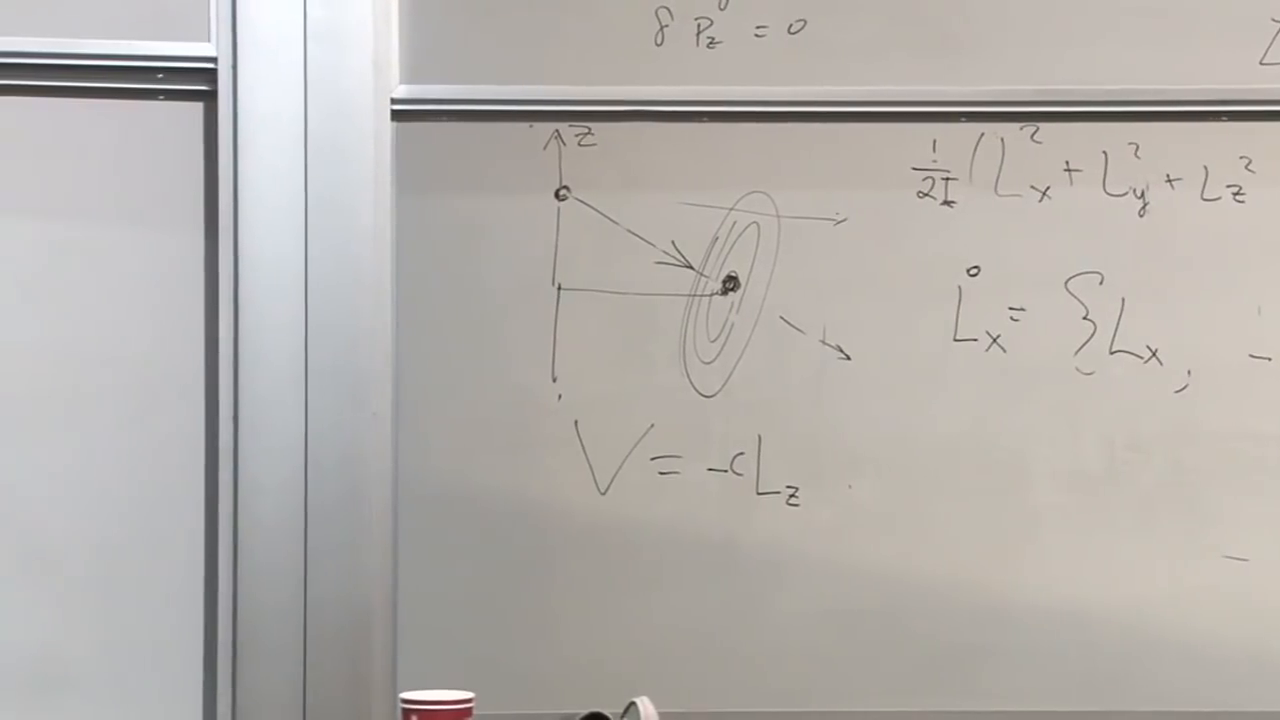
\includegraphics[width=0.82\textwidth]{lecture_08_figure_04.png}
  \caption{在由 \(L_z\) 生成的旋轉下，位置向量與動量向量依照相同的向量變換形式變化。}
  \lectureframe{00:42:08}
\end{figure}

因此，一般的哈密頓表述為
\begin{equation}
  \boxed{\delta_G A=\epsilon\{A,G\}.}
  \label{eq:l8-generator-rule}
\end{equation}
每個相空間函數 \(G\) 都會定義一個這樣的無窮小正則變換。若 \(G=L_z\)，這個變換就是旋轉；若 \(G=H\)，就是時間上的一小步。

\begin{classroomqa}
  \audiencequestion{本講有時談到旋轉系統，有時談到旋轉座標。括號方程採用哪一種約定？\lecturetimestamp{00:28:22--00:29:35}}
  \lecturerresponse{式 ~\eqref{eq:l8-z-rotation} 確立了約定：這裡採用的是無窮小主動旋轉 \((x,y)\mapsto(x-\epsilon y,y+\epsilon x)\)。若被動旋轉座標軸，符號則相反。約定一旦確立，括號公式便沒有歧義。}
\end{classroomqa}

\section{動量生成平移}

沿一個座標方向的平移為
\begin{equation}
  \delta q=\epsilon.
  \label{eq:l8-q-translation}
\end{equation}
在式 ~\eqref{eq:l8-noether-variation} 中，\(F(q)=1\)，因此相應的守恆量是 \(p\)。生成元的說法預測
\begin{equation}
  \{f(q),p\}=\frac{df}{dq}.
  \label{eq:l8-translation-derivative}
\end{equation}
本講先以歸納法證明這個結果適用於冪。基底情況為 \(\{q,p\}=1\)。假設
\begin{equation}
  \{q^{n-1},p\}=(n-1)q^{n-2}.
  \label{eq:l8-induction-hypothesis}
\end{equation}
那麼，根據乘積法則，
\begin{align}
  \{q^n,p\}
  &=\{q\,q^{n-1},p\}\\
  &=q\{q^{n-1},p\}+\{q,p\}q^{n-1}\\
  &=(n-1)q^{n-1}+q^{n-1}\\
  &=nq^{n-1}.
  \label{eq:l8-power-translation}
\end{align}
利用線性性，結果可推廣至多項式與收斂的冪級數表示。更直接地，從括號的定義可得，對每個可微函數 \(f(q)\)，式 ~\eqref{eq:l8-translation-derivative} 都成立：
\begin{equation}
  \{f(q),p\}
  =
  \frac{\partial f}{\partial q}
  \frac{\partial p}{\partial p}
  =f'(q).
\end{equation}

\begin{figure}[htbp]
  \centering
  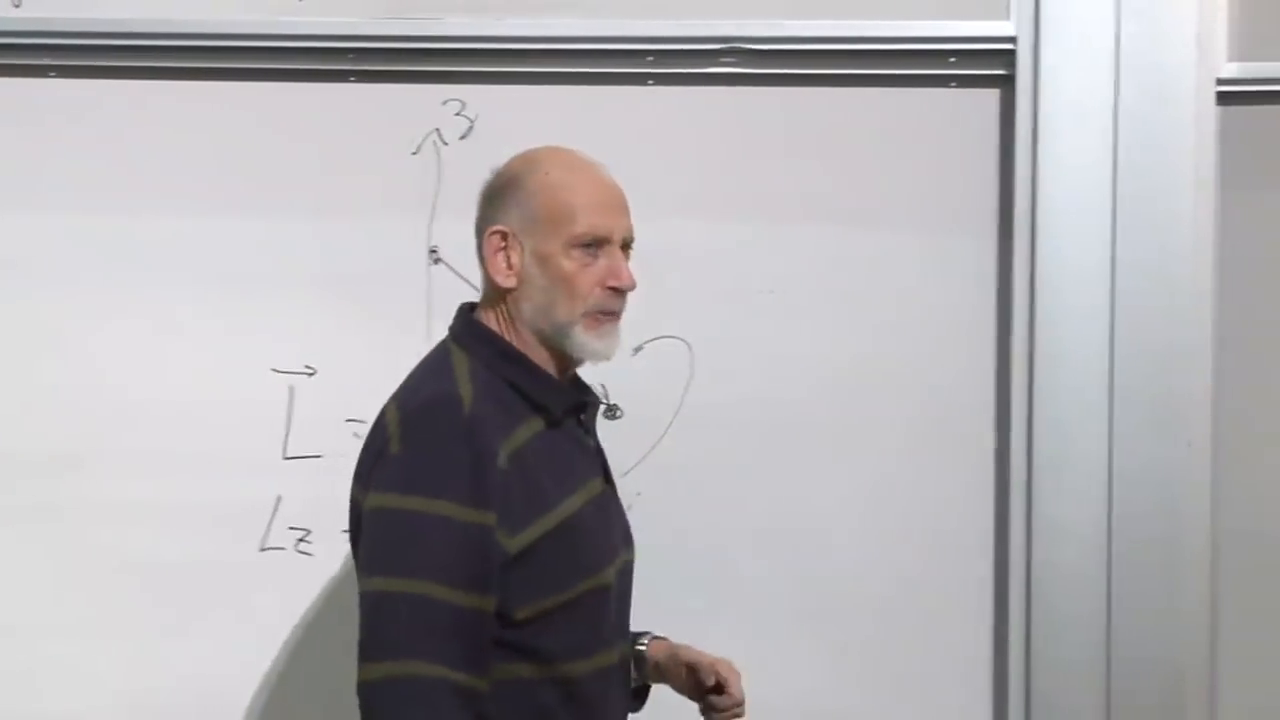
\includegraphics[width=0.82\textwidth]{lecture_08_figure_05.png}
  \caption{歸納證明後得到的平移結果：\(\{F(q),p\}=dF/dq\)。}
  \lectureframe{00:53:18}
\end{figure}

我們已經看到同一個觀念的三種形式：
\begin{center}
  \begin{tabular}{@{}>{\raggedright\arraybackslash}p{0.37\textwidth}
                      >{\raggedright\arraybackslash}p{0.55\textwidth}@{}}
    \toprule
    生成元與變換&無窮小作用\\
    \midrule
    \(H\)，時間平移& \(\delta_tA=\epsilon\{A,H\}\)\\
    \(p_i\)，空間平移& \(\delta A=\epsilon\{A,p_i\}\)\\
    \(L_i\)，旋轉& \(\delta A=\epsilon\{A,L_i\}\)\\
    \bottomrule
  \end{tabular}
\end{center}
與連續對稱性相應的守恆量，同時也是該對稱性的生成元。

\section{一個括號，兩種解讀}

設 \(G(q,p)\) 是候選生成元。若它是守恆量且不顯含時間，則
\begin{equation}
  \dot G=\{G,H\}=0.
  \label{eq:l8-g-conserved}
\end{equation}
由反對稱性可得
\begin{equation}
  \{H,G\}=0.
  \label{eq:l8-h-invariant}
\end{equation}
這兩個方程在數學上等價，但物理解讀不同：
\begin{itemize}
  \item \(\{G,H\}=0\) 表示 \(G\) 在由 \(H\) 生成的時間演化下不變。
  \item \(\{H,G\}=0\) 表示 \(H\) 在由 \(G\) 生成的變換下不變。
\end{itemize}
前者是守恆定律；後者是哈密頓量的對稱性。諾特定理所揭示的關聯，就濃縮在這個零值之中。

\begin{figure}[htbp]
  \centering
  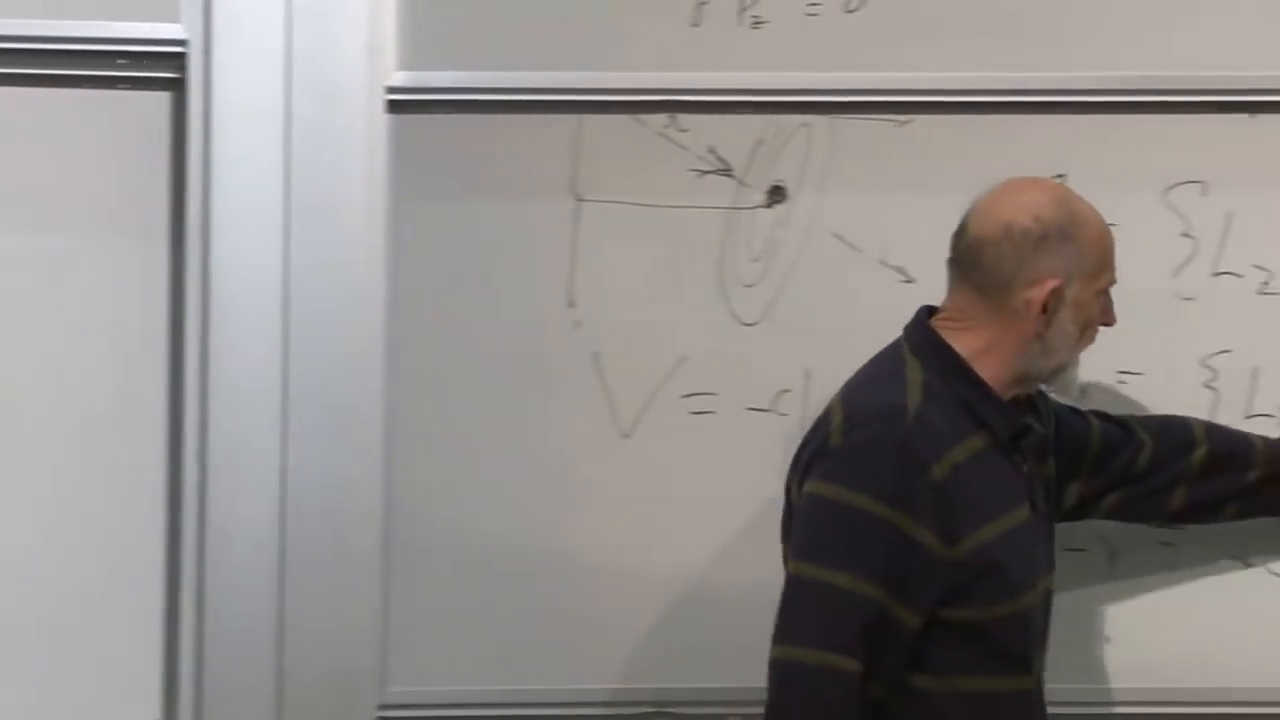
\includegraphics[width=0.82\textwidth]{lecture_08_figure_06.png}
  \caption{同一個零括號的兩種排列：\(G\) 守恆，以及 \(H\) 在由 \(G\) 生成的變換下保持不變。}
  \lectureframe{01:03:05}
\end{figure}

\begin{classroomqa}
  \audiencequestion{若已知某個守恆量，是否總能找出相應的對稱性？\lecturetimestamp{01:01:42--01:02:15}}
  \lecturerresponse{在這個哈密頓力學框架內，可以。將每個相空間變數與 \(G\) 取括號，所得的一組結果 \(\delta_GA=\epsilon\{A,G\}\) 會告訴我們這些變數如何變換。例如，與 \(L_z\) 取括號會顯示出旋轉，即使事先並不知道這種解讀。更進階的情況可能涉及整體性與邊界上的細節；此處使用的是局部的無窮小敘述。}
\end{classroomqa}

\begin{classroomqa}
  \audiencequestion{這些括號方程能告訴我們，究竟是哪種物理運動造成守恆定律嗎？
  \lecturetimestamp{00:56:01--00:58:13}}
  \lecturerresponse{不能。它們指出的是對稱變換，而不是實際軌跡。\(L_z\) 守恆表示系統具有旋轉對稱性，但不代表粒子沿圓周運動。實際的時間演化由 \(H\) 生成；與其他生成元取括號，則描述相空間中另一個方向的變換。}
\end{classroomqa}

\begin{classroomqa}
  \audiencequestion{有沒有不預先假設守恆的一般變換敘述？\lecturetimestamp{01:02:40--01:04:45}}
  \lecturerresponse{有。式 ~\eqref{eq:l8-generator-rule} 對每個函數 \(G\) 都定義了無窮小變換，不論它是否守恆。只有在哈密頓量保持不變時，這個變換才是對稱性：\(\{H,G\}=0\)。反過來讀取同一條件，就表示 \(G\) 是守恆量。}
\end{classroomqa}

\section{角動量代數}

接下來的計算讓我們在處理每個旋轉問題時，不必再逐一追蹤粒子座標。先從
\[
  L_x=yp_z-zp_y,\qquad
  L_z=xp_y-yp_x.
\]
開始。在 \(\{L_x,L_z\}\) 中，大多數交叉項都會消失，因為它們的指標並未形成正則共軛對。留下的縮併項給出
\begin{align}
  \{L_x,L_z\}
  &=\{yp_z-zp_y,xp_y-yp_x\}\\
  &=xp_z-zp_x\\
  &=-L_y.
  \label{eq:l8-lx-lz}
\end{align}
交換括號內兩項的次序，負號便消失。依序輪換座標，可得
\begin{equation}
  \boxed{\begin{aligned}
    \{L_x,L_y\}&=L_z,\\
    \{L_y,L_z\}&=L_x,\\
    \{L_z,L_x\}&=L_y.
  \end{aligned}}
  \label{eq:l8-angular-algebra}
\end{equation}
用指標表示則為
\begin{equation}
  \{L_i,L_j\}=\varepsilon_{ijk}L_k.
  \label{eq:l8-angular-algebra-index}
\end{equation}

\begin{figure}[htbp]
  \centering
  \includegraphics[width=0.82\textwidth]{lecture_08_figure_07.png}
  \caption{三個角動量分量的循環泊松括號代數。}
  \lectureframe{01:10:52}
\end{figure}

這個結果其實也可以預見。既然 \(\boldsymbol L\) 是向量，將它的 \(x\) 分量與 \(L_z\) 取括號，必定會得到該分量在繞 \(z\) 軸旋轉時的無窮小變化，也就是 \(-L_y\)。明確計算驗證了這個幾何論證。這些方程也是量子角動量對易關係的經典前身。

\section{快速旋轉的陀螺}

作為應用，考慮一個陀螺：飛輪快速旋轉，其中心與支點相距 \(R\)。令 \(\boldsymbol r\) 表示從支點指向輪心的向量。飛輪繞軸高速自轉，因此主要角動量保持與該方向平行。在本講採用的近似下，
\begin{equation}
  \boldsymbol L=\ell\,\boldsymbol r,
  \qquad
  L_z=\ell z,
  \label{eq:l8-L-parallel-r}
\end{equation}
其中 \(\ell=L/R\) 視為常數。起初先忽略與章動或轉軸運動相關的較小角動量。

\begin{figure}[htbp]
  \centering
  \begin{tikzpicture}[scale=0.95,>=Latex]
    \coordinate (P) at (0,3.2);
    \coordinate (C) at (3.7,1.55);
    \draw[->] (0,-0.2) -- (0,4.35) node[above] {\(z\)};
    \fill (P) circle (1.7pt) node[left] {pivot};
    \draw[very thick,->] (P) -- (C)
      node[midway,above right] {\(\boldsymbol r\parallel\boldsymbol L\)};
    \fill (C) circle (1.7pt);
    \draw[dashed] (P) -- (0,1.55);
    \draw[dashed] (0,1.55) -- (C);
    \node[left] at (0,1.55) {\(z\)};
    \begin{scope}[shift={(C)},rotate=-24]
      \draw[very thick] (0,0) ellipse (0.65 and 1.35);
      \draw[thick] (0,0) ellipse (0.42 and 0.9);
    \end{scope}
    \draw[->,thick] (2.15,2.85)
      arc[start angle=140,end angle=35,radius=1.65];
  \end{tikzpicture}
  \caption{快速陀螺近似：支點至輪心的距離固定，主要自轉角動量保持與轉軸及 \(\boldsymbol r\) 平行。}
\end{figure}

\begin{figure}[htbp]
  \centering
  \includegraphics[width=0.82\textwidth]{lecture_08_figure_08.png}
  \caption{黑板上的飛輪示意圖，並列出 \(H_{\rm rot}=L^2/(2I)\)；其中的抵消說明了無力矩時 \(\boldsymbol L\) 守恆。}
  \lectureframe{01:18:54}
\end{figure}

\subsection{無重力時：為何每個分量都保持不變}

對簡化的軸對稱轉子而言，
\begin{equation}
  H_{\mathrm{rot}}
  =\frac{1}{2I}
  \left(L_x^2+L_y^2+L_z^2\right)
  =\frac{L^2}{2I}.
  \label{eq:l8-rotational-hamiltonian}
\end{equation}
係數應為 \(1/(2I)\)，而非 \(I/2\)；講者在黑板上寫錯後隨即更正。利用式 ~\eqref{eq:l8-angular-algebra}，
\begin{align}
  \dot L_x
  &=\{L_x,H_{\mathrm{rot}}\}\\
  &=\frac{1}{2I}\left(
    2L_y\{L_x,L_y\}
    +2L_z\{L_x,L_z\}
  \right)\\
  &=\frac{1}{I}\left(L_yL_z-L_zL_y\right)=0.
  \label{eq:l8-free-lx}
\end{align}
循環置換各分量，可得
\begin{equation}
  \dot L_x=\dot L_y=\dot L_z=0.
  \label{eq:l8-free-angular-momentum}
\end{equation}
純量 \(L^2\) 與每個分量 \(L_i\) 的括號都為零；依這套代數的術語，它是卡西米爾量。因此，無力矩作用的陀螺，其角動量的大小與方向都保持不變。

\begin{classroomqa}
  \audiencequestion{這裡的轉動慣量只是純量嗎？
  \lecturetimestamp{01:14:23--01:15:05}}
  \lecturerresponse{對這個簡化模型來說，是的。它描述飛輪繞自轉軸的質量分布。一般剛體則有轉動慣量張量，而在主軸座標系中，轉動哈密頓量為 \(\sum_i L_i^2/(2I_i)\)。本講選用較簡單的高速對稱轉子，目的是展示泊松括號方法，而非完整探討剛體動力學。}
\end{classroomqa}

\subsection{重力與位能的符號}

令垂直座標 \(z\) 向上為正，並將支點設在原點。輪心的重力位能為
\begin{equation}
  V=Mgz.
  \label{eq:l8-mgz}
\end{equation}
由於 \(L_z=\ell z\)，
\begin{equation}
  V=cL_z,
  \qquad
  c=\frac{Mg}{\ell}=\frac{MgR}{L}.
  \label{eq:l8-potential-lz}
\end{equation}
當 \(\boldsymbol L\) 的方向與 \(\boldsymbol r\) 平行時，這裡有 \(c>0\)。若飛輪以相反方向自轉，\(\boldsymbol L\) 與 \(\boldsymbol r\) 之間的帶符號比例關係會反轉，相應的帶符號進動頻率也會反轉。

\begin{figure}[htbp]
  \centering
  \includegraphics[width=0.82\textwidth]{lecture_08_figure_09.png}
  \caption{定長幾何所導出的關係：\(\boldsymbol L=\ell\boldsymbol r\) 與 \(L_z=\ell z\)。}
  \lectureframe{01:25:38}
\end{figure}

\begin{figure}[htbp]
  \centering
  \includegraphics[width=0.82\textwidth]{lecture_08_figure_10.png}
  \caption{黑板上的中間推導曾寫成 \(V=-cL_z\)。後來確定 \(z\) 向上為正後，修正了符號：當 \(\boldsymbol L=\ell\boldsymbol r\) 且 \(\ell>0\) 時，一致的結果是 \(V=+cL_z\)。}
  \lectureframe{01:22:43}
\end{figure}

\begin{classroomqa}
  \audiencequestion{為什麼可以用角動量的一個分量取代高度？那條斜線代表轉軸，還是位置向量？
  \lecturetimestamp{01:22:20--01:25:43}}
  \lecturerresponse{那條斜線最好標為 \(\boldsymbol r\)，也就是從固定支點指向輪心的向量。實際轉軸可能沿著這個方向，但計算所用的關係是快速自轉近似 \(\boldsymbol L=\ell\boldsymbol r\)，因此兩者的 \(z\) 分量成正比。課堂討論曾多次更改標記，最後才確立這項區分。}
\end{classroomqa}

\begin{classroomqa}
  \audiencequestion{哪些假設使 \(\ell\) 保持不變？若輪心能沿徑向滑動，會有什麼問題？
  \lecturetimestamp{01:25:43--01:26:38,\allowbreak\ 01:34:22--01:35:00}}
  \lecturerresponse{假設主要自轉角動量遠大於慢速運動所帶來的角動量，並且支點至輪心的距離固定。如此一來，自轉角動量的大小變化不大，而 \(\boldsymbol L\) 會隨 \(\boldsymbol r\) 一起轉動。若輪心能沿徑向滑動，\(z\) 就不再以固定比例係數與 \(L_z\) 成正比，因此簡化哈密頓量 \(V=cL_z\) 將無法描述其運動。}
\end{classroomqa}

\begin{classroomqa}
  \audiencequestion{為什麼黑板上起初寫負號，後來又改成正號？自轉方向有影響嗎？
  \lecturetimestamp{01:27:13--01:28:15,\allowbreak\ 01:33:09--01:33:21}}
  \lecturerresponse{起初的符號是黑板推導中的錯誤，也混入了尚未確定的軸方向約定。一旦定義 \(z\) 向上，位能 \(V=Mgz\) 就隨高度增加。若 \(\boldsymbol L=\ell\boldsymbol r\) 且 \(\ell>0\)，便得到 \(V=+cL_z\)。反轉自轉方向會使帶符號的比例關係與進動方向反轉，但符號不能任意選取。}
\end{classroomqa}

\subsection{由三個簡短方程導出進動}

完整的簡化哈密頓量為
\begin{equation}
  H=
  \frac{1}{2I}\left(L_x^2+L_y^2+L_z^2\right)+cL_z.
  \label{eq:l8-full-gyro-hamiltonian}
\end{equation}
我們已經證明 \(L^2\) 與每個 \(L_i\) 的括號都為零。因此只有線性項有貢獻：
\begin{align}
  \dot L_z&=\{L_z,H\}=0,\\
  \dot L_x&=\{L_x,H\}=c\{L_x,L_z\}=-cL_y,\\
  \dot L_y&=\{L_y,H\}=c\{L_y,L_z\}=cL_x.
  \label{eq:l8-precession-equations}
\end{align}

\begin{figure}[htbp]
  \centering
  \includegraphics[width=0.82\textwidth]{lecture_08_figure_11.png}
  \caption{最後得到的分量方程：\(L_z\) 保持不變，而 \(L_x\) 與 \(L_y\) 彼此轉換。}
  \lectureframe{01:30:35}
\end{figure}

垂直分量與水平分量的大小都保持不變：
\begin{equation}
  \frac{d}{dt}(L_x^2+L_y^2)
  =2L_x(-cL_y)+2L_y(cL_x)=0.
\end{equation}
合併水平分量，得到
\begin{equation}
  L_+=L_x+iL_y,
  \qquad
  \dot L_+=icL_+,
\end{equation}
因此
\begin{equation}
  L_+(t)=L_+(0)e^{ict}.
  \label{eq:l8-precession-solution}
\end{equation}
角動量向量便以角速度 \(|c|=MgR/L\) 繞垂直軸進動。在這個理想化的定常運動中，其傾角保持不變。

\begin{classroomqa}
  \audiencequestion{寫出進動方程時，轉動能項有被忽略嗎？
  \lecturetimestamp{01:35:01--01:35:49}}
  \lecturerresponse{沒有。它包含在完整哈密頓量中，如式 ~\eqref{eq:l8-full-gyro-hamiltonian} 所示。它對 \(\dot L_i\) 的貢獻為零，因為 \(\{L_i,L^2\}=0\)；這項抵消已在無力矩的計算中證明。學生的提問讓這個原本隱含的步驟明確呈現出來。}
\end{classroomqa}

\begin{classroomqa}
  \audiencequestion{等速進動算是一種平衡嗎？受到輕微擾動後會如何？\lecturetimestamp{01:32:38--01:33:08}}
  \lecturerresponse{與其稱為靜態平衡，不如稱為穩態運動或定常運動。輕微擾動通常會引入章動，也就是傾角的振盪。飛輪自轉得非常快時，振盪幅度很小，因此簡化分析只考慮近似等速的進動。}
\end{classroomqa}

\begin{classroomqa}
  \audiencequestion{進動一定需要支架或實際的轉軸嗎？
  \lecturetimestamp{01:31:49--01:32:38,\allowbreak\ 01:33:49--01:35:00}}
  \lecturerresponse{這個力學模型假設支點至輪心的距離固定，因此必須有某種約束提供支撐。更一般的代數結果則是：只要哈密頓量中有一項與角動量的某個分量成正比，同樣的括號代數便會導出進動。角動量的微觀來源不一定是實際裝在轉軸上的輪子。}
\end{classroomqa}

\begin{classroomqa}
  \audiencequestion{這和磁場中的電子自旋或核自旋進動，或行星軌道進動，是同一種現象嗎？
  \lecturetimestamp{01:35:50--01:37:00}}
  \lecturerresponse{磁矩與磁場耦合時，哈密頓量會與自旋的一個分量成正比，因此遵循相同的角動量代數。核自旋進動是核磁共振的基礎。行星軌道近日點的進動則是另一種現象，只是也使用「\emph{進動}」一詞；兩者的計算並不相同。}
\end{classroomqa}

\begin{classroomqa}
  \audiencequestion{側向安裝的陀螺儀，基本上和旋轉陀螺是同一種物體嗎？\lecturetimestamp{01:37:02--01:37:23}}
  \lecturerresponse{是。兩者的差別主要在幾何上的稱呼：自轉軸從支座向側方伸出時，通常稱為陀螺儀；自轉軸接近垂直時，則通常稱為陀螺。它們的角動量與力矩結構相同。}
\end{classroomqa}

\section{這項計算的成果}

整個過程沒有引入尤拉角，也沒有追蹤飛輪各部分的座標。一旦知道 \[
  \{L_i,L_j\}=\varepsilon_{ijk}L_k
\]，便能直接得到所關心變數的方程。這正是本講要展示的威力。諧振子說明泊松括號可以重現熟悉的動力學；角動量則顯示它們的用途遠不止於此：
\begin{itemize}
  \item 守恆量會生成與之相應的無窮小對稱性；
  \item  \(G\) 的守恆與 \(H\) 的不變性，是 \(\{G,H\}=0\) 的兩種解讀；
  \item 可觀測量的代數可以形成封閉系統，讓我們不必回到微觀座標就能求解動力學；
  \item 哈密頓量若與角動量的一個分量成正比，就會產生繞該軸的進動。
\end{itemize}
本講尚未推導一般剛體的完整尤拉方程，但較為聚焦的結論已經完整：選對生成元並運用其泊松代數，就能以極精簡的方式揭示對稱性與運動。
\chapter{磁力、向量位勢與作用量原理}

\lectureoverview{靜電力符合熟悉的保守力形式，但磁力取決於速度。為了將磁力納入拉格朗日力學，我們先介紹所需的向量微積分，利用磁場無源的性質引入向量位勢，探討其規範自由度，接著在作用量中建構磁力項。}

\section{一種新型態的力}

前面討論角動量、陀螺儀與泊松括號時，幾個主題彼此連結了起來。特別是，帶電剛體在磁場中旋轉時，會像陀螺儀一樣進動。現在我們從這個類比轉向單一帶電粒子的運動。

靜電力不需要新的力學。若 \(U(\mathbf x)\) 是位能，則
\begin{equation}
  \mathbf F=-\nabla U(\mathbf x),
\end{equation}
通常的論證便可得出動能與位能之和守恆。對於電荷為 \(e\)、處於靜電位勢 \(V(\mathbf x)\) 中的粒子，
\begin{equation}
  U(\mathbf x)=eV(\mathbf x),
  \qquad
  \mathbf F_{\mathrm{el}}=-e\nabla V.
\end{equation}
磁力的形式則不同。磁力取決於粒子的速度，因此不能只靠加入另一個一般位能來描述。儘管如此，磁力確實可以由作用量原理導出，也能以拉格朗日與哈密頓形式描述。要建立這種描述，我們得先簡短但不可或缺地插入一段向量微積分。

\section{場與局域運算}

\subsection{場所記錄的量}

場在空間的每一點（一般而言，也在每一時刻）指定一個物理量。溫度與壓力是標量場；風的速度是向量場。電場與磁場也是向量場。其他理論甚至在微觀尺度上也包含標量場，而引力則以張量場描述。在目前的討論中，我們先略去時間依賴，將場寫成 \(\mathbf x\) 的函數。

場在操作上的意義在於局域性。設想某個區域被藏在袋子裡。若要測量該區域中的電場，就在那裡放入一個小型試驗電荷，觀察它的加速度。電荷所受的力由它所在位置的場決定，不必另外逐一詢問每個遠處的源。磁場對運動試驗電荷也適用同樣的說法。稍後，向量位勢會使我們需要修正這幅簡單圖像，但它仍是恰當的出發點。

\subsection{微分算符}

微分會將場轉換成其他場。我們把三個空間微分合寫為
\begin{equation}
  \nabla
  =
  \left(
    \frac{\partial}{\partial x},
    \frac{\partial}{\partial y},
    \frac{\partial}{\partial z}
  \right).
\end{equation}
這個符號讀作 \emph{del} 或 \emph{nabla}。它倒三角形的外觀令人印象深刻，但真正重要的是，它在形式上像一個向量，其分量是微分算符。

這裡談的是普通的三維物理空間，不是相空間，也不是多粒子組態空間。此外，\(\nabla\) 並不是能獨立存在的向量場；它必須作用在某個對象上。若 \(T(\mathbf x)\) 是標量溫度場，則
\begin{equation}
  \nabla T
  =
  \left(
    \frac{\partial T}{\partial x},
    \frac{\partial T}{\partial y},
    \frac{\partial T}{\partial z}
  \right)
\end{equation}
就是它的梯度，也是真正的向量場。

\begin{figure}[htbp]
\centering
\includegraphics[width=0.82\textwidth]{lecture_09_figure_01.png}
\caption{黑板上先將 \(\nabla\) 引入為由空間微分算符構成的向量，接著示範它如何作用於標量場 \(T(\mathbf x)\)。}
\lectureframe{00:11:30}
\end{figure}

標量不只是以單一分量表示的量；它的數值不因座標軸的取向而改變。溫度就是典型例子。給定向量場 \(\mathbf E\)，局域量 \(\mathbf E\cdot\mathbf E\) 也是一個標量。相較之下，藉由積分場來構造位勢是一種非局域運算，因為它會用到沿途的場值。

\subsection{散度}

對於向量場 \(\mathbf A=(A_x,A_y,A_z)\)，標量
\begin{equation}
  \nabla\cdot\mathbf A
  =
  \frac{\partial A_x}{\partial x}
  +\frac{\partial A_y}{\partial y}
  +\frac{\partial A_z}{\partial z}
\end{equation}
稱為它的散度。用流體來說，正散度表示流體在局部有向外流出的趨勢，負散度則表示有向內匯聚的趨勢。流體的源會產生正散度，匯則產生負散度。這只是定性的圖像，但足以清楚說明磁場無源的性質。

\section{叉積、epsilon 符號與旋度}

\subsection{叉積的分量表示法}

對於兩個向量 \(\mathbf V\) 與 \(\mathbf A\)，叉積的一個分量是
\begin{equation}
  (\mathbf V\times\mathbf A)_x
  =
  V_yA_z-V_zA_y.
\end{equation}
另外兩個分量可依照 \(x\to y\to z\to x\) 的循環順序寫出。將 \(x,y,z\) 換成指標 \(1,2,3\) 會更方便。克羅內克符號定義為
\begin{equation}
  \delta_{ij}
  =
  \begin{cases}
    1,&i=j,\\
    0,&i\ne j,
  \end{cases}
\end{equation}
而 Levi--Civita 符號定義為
\begin{equation}
  \epsilon_{123}=\epsilon_{231}=\epsilon_{312}=1,
  \qquad
  \epsilon_{132}=\epsilon_{321}=\epsilon_{213}=-1,
\end{equation}
只要有任意兩個指標相同，便有 \(\epsilon_{ijk}=0\)。沿三點鐘方向循環排列時，符號為正；反向排列時，符號為負。交換任意一對指標都會使符號反轉，因此 \(\epsilon_{ijk}\) 完全反對稱。

我們也採用求和慣例：一個項中重複出現的指標，表示從 \(1\) 到 \(3\) 求和。於是，三個叉積方程可合寫為
\begin{equation}
  (\mathbf V\times\mathbf A)_i
  =
  \epsilon_{ijk}V_jA_k.
\end{equation}
例如，令 \(i=1\)，只剩下 \((j,k)=(2,3)\) 與 \((3,2)\)：
\begin{equation}
  (\mathbf V\times\mathbf A)_1
  =
  \epsilon_{123}V_2A_3
  +\epsilon_{132}V_3A_2
  =
  V_2A_3-V_3A_2.
\end{equation}
因此，這種簡潔記法完整保留了熟悉的分量公式。

\subsection{以反對稱矩陣表示的向量}

還有另一種表示法：
\begin{equation}
  V_iA_j-V_jA_i
  =
  \epsilon_{ijk}(\mathbf V\times\mathbf A)_k.
\end{equation}
左側有兩個指標，並在 \(i\leftrightarrow j\) 下呈反對稱。寫成矩陣時，形式如下：
\begin{equation}
  M_{ij}
  =
  \begin{pmatrix}
    0&M_{12}&M_{13}\\
    -M_{12}&0&M_{23}\\
    -M_{13}&-M_{23}&0
  \end{pmatrix}.
\end{equation}
對角線元素為零，下三角部分由上三角部分決定，因此只有三個獨立分量。

\begin{figure}[htbp]
\centering
\includegraphics[width=0.82\textwidth]{lecture_09_figure_02.png}
\caption{一個叉積分量，以及用來計算其獨立元素數目的示意性 \(3\times3\) 反對稱陣列。格子中的標記只是助記符號，並非額外的符號。}
\lectureframe{00:34:20}
\end{figure}

\begin{classroomqa}
\audiencequestion{叉積，或是把它辨認為另一個向量的做法，在三維以外也有意義嗎？}
\lecturerresponse{反對稱的二階張量在任何維度都有意義，但把它辨認為向量則是三維的特殊性。三維向量有三個分量，反對稱的 \(3\times3\) 矩陣也有三個獨立分量。到了四維，相應的數目是四與六，因為 \(4(4-1)/2=6\)。反對稱的對象依然存在，而且自然地可視為二形式，但它並不是另一個四維向量。}
\end{classroomqa}

\subsection{旋度}

將 \(\mathbf V\) 換成 \(\nabla\)，便定義了旋度：
\begin{equation}
  (\nabla\times\mathbf A)_i
  =
  \epsilon_{ijk}\frac{\partial A_k}{\partial x_j}.
\end{equation}
以一般分量表示，
\begin{align}
  (\nabla\times\mathbf A)_x
  &=
  \frac{\partial A_z}{\partial y}
  -\frac{\partial A_y}{\partial z},\\
  (\nabla\times\mathbf A)_y
  &=
  \frac{\partial A_x}{\partial z}
  -\frac{\partial A_z}{\partial x},\\
  (\nabla\times\mathbf A)_z
  &=
  \frac{\partial A_y}{\partial x}
  -\frac{\partial A_x}{\partial y}.
\end{align}
散度描述局部的發散，旋度則描述局部的環流。流體若繞著某個軸旋轉，沿該軸的旋度就不為零。這個圖像用在速度場上特別直觀，但旋度的定義適用於任何向量場。

\section{兩個結構恆等式}

以下兩個性質幾乎涵蓋了全部數學工作：
\begin{equation}
  \nabla\cdot(\nabla\times\mathbf A)=0,
  \qquad
  \nabla\times(\nabla s)=0.
\end{equation}
第一個成立，是因為二階微分的次序可以交換，而 \(\epsilon_{ijk}\) 是反對稱的：
\begin{equation}
  \nabla\cdot(\nabla\times\mathbf A)
  =
  \epsilon_{ijk}\partial_i\partial_j A_k
  =0.
\end{equation}
第二個則來自混合偏導數相等：
\begin{equation}
  \bigl[\nabla\times(\nabla s)\bigr]_i
  =
  \epsilon_{ijk}\partial_j\partial_k s
  =0.
\end{equation}

\begin{figure}[htbp]
\centering
\includegraphics[width=0.80\textwidth]{lecture_09_figure_03.png}
\caption{黑板上的第一個恆等式：任何旋度的散度都為零。}
\lectureframe{00:38:26}
\end{figure}

這兩個方向的證明都很簡單，正好適合作為講課中提到的作業或隨堂測驗。逆命題則需要更仔細處理。在局部，或在適當的單連通或可縮區域上作整體考量時，
\begin{align}
  \nabla\cdot\mathbf F=0
  &\quad\Longrightarrow\quad
  \mathbf F=\nabla\times\mathbf A,\\
  \nabla\times\mathbf F=0
  &\quad\Longrightarrow\quad
  \mathbf F=\nabla s.
\end{align}
若不加上區域條件，孔洞等整體拓撲特徵可能使這些結論不成立。以下只會用到講課所採用的局部形式。

\section{為什麼磁場可以寫成旋度}

\subsection{沒有觀測到磁源}

磁場 \(\mathbf B\) 是透過它對帶電粒子與電流的作用來操作性定義的。在沒有磁單極子的普通電磁學中，
\begin{equation}
  \nabla\cdot\mathbf B=0.
\end{equation}
這與電場不同，電場的散度正比於電荷密度。電荷是電通量的源或匯；至今尚未觀測到孤立的磁通量源或匯。

若存在磁單極子，這個方程就會改變。統一場論通常提供理論上的理由，預期這類物體可能存在；但即使存在，它們的質量也可能大到目前的實驗無法產生。因此，現行理論採用磁荷密度為零的假設。

\begin{classroomqa}
\audiencequestion{磁單極子會是什麼？普通磁鐵不是已經有北極和南極了嗎？}
\lecturerresponse{孤立的磁單極子會是真正的磁場源或匯，類似電荷。普通條形磁鐵則不同：從北極附近出發的場線會彎曲穿過空間，再由南極返回，並繼續穿過磁鐵材料。外觀看似源與匯的兩端其實彼此相連，就像流體經由看不見的管道流動。磁通量並沒有淨生成或消失。}
\end{classroomqa}

\begin{figure}[htbp]
\centering
\includegraphics[width=0.76\textwidth]{lecture_09_figure_04.png}
\caption{黑板上對照了看似存在的北極源與南極匯，並將場線畫成穿過磁鐵彼此相連，以強調磁通量並未在兩極起始或終止。}
\lectureframe{00:44:56}
\end{figure}

由於 \(\mathbf B\) 的散度為零，利用逆命題，至少在局部可以寫成
\begin{equation}
  \boxed{\mathbf B=\nabla\times\mathbf A}.
\end{equation}
場 \(\mathbf A\) 稱為向量位勢。乍看之下，這似乎只是以另一種方式描述可測量的場 \(\mathbf B\)，但它的用途要等到建構作用量時才會明朗。

\subsection{向量位勢並不唯一}

若 \(\mathbf A\) 是一個向量位勢，那麼
\begin{equation}
  \mathbf A'=\mathbf A+\nabla s
\end{equation}
也是另一個向量位勢，因為
\begin{equation}
  \nabla\times\mathbf A'
  =
  \nabla\times\mathbf A+\nabla\times(\nabla s)
  =
  \mathbf B.
\end{equation}
這種替換稱為\emph{規範變換}。磁場在規範變換下保持不變。

\begin{figure}[htbp]
\centering
\includegraphics[width=0.80\textwidth]{lecture_09_figure_05.png}
\caption{黑板上同時寫出定義關係 \(\mathbf B=\nabla\times\mathbf A\) 與規範變換 \(\mathbf A'=\mathbf A+\nabla s\)。}
\lectureframe{01:03:01}
\end{figure}

這個字讀作 \emph{gauge}，不是 \emph{gouache}，也不是 \emph{gouge}--——講課時還半開玩笑地嚴格強調了這項區別。這個詞有其歷史由來。它源自早期一種嘗試，試圖將這種自由度與不同位置間長度標準的比較連結起來。原先的詮釋沒有保留下來，但名稱沿用至今。

\begin{classroomqa}
\audiencequestion{在這裡，規範變換是否專指 \(\mathbf A\mapsto\mathbf A+\nabla s\)？}
\lecturerresponse{是的，這就是此處使用的完整電磁規範變換。Yang--Mills 理論及其他場論中的規範變換，是同一概念的推廣；但電磁學只需加上一個標量梯度。}
\end{classroomqa}

向量位勢的不唯一性也說明了哪些量可以直接測量。小區域中的帶電粒子會受到局部 \(\mathbf B\) 的作用，而所有透過規範變換彼此相連的向量位勢，對該處的力都會作出相同預測。這類經典局域實驗無法為 \(\mathbf A\) 指定唯一的數值。

\begin{classroomqa}
\audiencequestion{加上一個梯度，是否就完整描述了這種不唯一性？}
\lecturerresponse{在簡單區域的局部範圍內，是的。若 \(\nabla\times\mathbf A'=\nabla\times\mathbf A\)，則 \(\nabla\times(\mathbf A'-\mathbf A)=0\)，因此兩者之差是某個梯度。從整體來看，多連通區域可能還有其他微妙之處。加上一個常向量也已包含在這種形式中，因為常向量是某個線性標量函數的梯度。若對 \(s\) 本身加上一個常數，則不會造成任何改變，因為它的梯度為零。}
\end{classroomqa}

\begin{classroomqa}
\audiencequestion{如果規範自由度背後有物理原因，那是什麼？}
\lecturerresponse{講課中暫且不談這個更深層的詮釋。眼下有用的第一步，是先運用這種自由度，看看它如何進入作用量。熟悉這套形式之後，規範描述何以不可或缺，就會更容易理解。}
\end{classroomqa}

\section{一個磁場，多種位勢}

考慮最簡單的例子：
\begin{equation}
  \mathbf B=b\,\hat{\mathbf z},
  \qquad
  B_x=B_y=0,
  \qquad
  B_z=b,
\end{equation}
其中 \(b\) 是常數。一個向量位勢為
\begin{equation}
  \mathbf A^{(1)}=(0,bx,0).
\end{equation}
確實，
\begin{equation}
  (\nabla\times\mathbf A^{(1)})_z
  =
  \frac{\partial A_y^{(1)}}{\partial x}
  -\frac{\partial A_x^{(1)}}{\partial y}
  =b,
\end{equation}
而旋度的其他分量皆為零。

這種選擇似乎特別指定了 \(y\) 方向，儘管物理磁場在 \(x\)-\(y\) 平面內具有旋轉對稱性。另一種選擇則讓這種任意性更明顯：
\begin{equation}
  \mathbf A^{(2)}=(-by,0,0).
\end{equation}
其旋度為
\begin{equation}
  (\nabla\times\mathbf A^{(2)})_z
  =
  0-\frac{\partial(-by)}{\partial y}
  =b.
\end{equation}
兩種位勢之差為
\begin{equation}
  \mathbf A^{(2)}-\mathbf A^{(1)}
  =
  (-by,-bx,0)
  =
  \nabla(-bxy).
\end{equation}
因此兩者規範等價。具有旋轉對稱性的選擇
\begin{equation}
  \mathbf A^{(\mathrm{sym})}
  =
  \frac12\,\mathbf B\times\mathbf r
  =
  \left(-\frac{by}{2},\frac{bx}{2},0\right),
\end{equation}
也是同一族中的另一個成員。

\begin{figure}[htbp]
\centering
\includegraphics[width=0.80\textwidth]{lecture_09_figure_06.png}
\caption{黑板的兩個區塊分別列出選擇 \(A_y=bx\) 與 \(A_x=-by\)，兩者都產生相同的均勻磁場 \(B_z=b\)。}
\lectureframe{01:07:20}
\end{figure}

\begin{classroomqa}
\audiencequestion{這種模糊性，是否等同於用不同方式配置載流線圈來產生磁場？}
\lecturerresponse{不是。不同的電流配置代表不同的物理源，即使它們在某個區域內產生相同的磁場，在其他地方仍可能產生不同的磁場。即使磁場已在所有地方完全指定，規範自由度依然存在：同一個物理磁場 \(\mathbf B\) 仍可由多種向量位勢描述。}
\end{classroomqa}

\begin{classroomqa}
\audiencequestion{能不能把加上梯度想成拉伸或壓縮，但不增加扭轉？}
\lecturerresponse{這是有用的幾何直覺。旋度反映局部的扭轉部分，而純梯度的旋度為零。這項敘述精確地表現在 \(\nabla\times\nabla s=0\) 中。}
\end{classroomqa}

\begin{classroomqa}
\audiencequestion{\(\mathbf A\) 的方向與 \(\mathbf B\) 的方向之間，有固定的關係嗎？}
\lecturerresponse{不存在與規範選擇無關的固定關係。上述例子恰好滿足 \(A_z=0\)，但可以再加上一個常數 \(A_z\)，而不改變任何微分。如此一來，\(\mathbf A\) 就不再垂直於 \(\mathbf B\)。在這段經典討論中，只有旋度具有不變的物理意義。}
\end{classroomqa}

靜電學中也有較簡單的類似情形。由於 \(\mathbf E=-\nabla V\)，將 \(V\) 換成 \(V+C\) 不會改變 \(\mathbf E\)。選用\emph{向量位勢}這個名稱，部分原因是它類比了普通標量位勢的這種自由度：我們可以用某種方式改變位勢，而不改變物理場。

\section{洛倫茲力}

現在可以寫出作用量原理必須導出的力定律。依照此處採用的慣例，
\begin{equation}
  \boxed{
  \mathbf F
  =
  e\left(
    \mathbf E+\frac{\mathbf v}{c}\times\mathbf B
  \right)
  =
  -e\nabla V+\frac{e}{c}\mathbf v\times\mathbf B
  }.
\end{equation}
符號 \(e\) 代表粒子的電荷，\(\mathbf v=\dot{\mathbf x}\) 代表粒子的速度，\(V\) 則是標量位勢。不要因此把 \(V\) 和 \(\mathbf v\) 混為一談。以 SI 制表示，\(V\) 的單位是伏特，\(e\) 的單位是庫侖；式中的 \(1/c\) 則來自講課採用的單位慣例。物理結構上的重點不受單位制影響。

\begin{figure}[htbp]
\centering
\includegraphics[width=0.82\textwidth]{lecture_09_figure_07.png}
\caption{黑板上並列展示洛倫茲力的電場項與磁場項。磁力項正比於 \(\mathbf v\times\mathbf B\)。}
\lectureframe{00:58:54}
\end{figure}

電場項是保守力，我們已經熟悉；磁場項則是新的。粒子靜止時，磁力項為零，而且磁力同時垂直於 \(\mathbf v\) 與 \(\mathbf B\)。因此，
\begin{equation}
  \mathbf v\cdot\mathbf F_{\mathrm{mag}}
  =
  \frac{e}{c}\mathbf v\cdot(\mathbf v\times\mathbf B)
  =0.
\end{equation}
靜磁場會使粒子的軌跡彎曲，卻不對粒子作功。這與黏滯阻力不同，後者方向與速度相反，並會減少動能。

因子 \(v/c\) 也顯示，依照此處的單位慣例，當場的尺度相當時，慢速粒子受到的磁效應通常小於電效應。電子質量很小，能達到很高的速率，因此磁偏轉仍然很容易觀測。

歷史上，人們先知道載流導線會受力，之後才辨認出單一電荷所受的力。Lorentz 認為，只要把依賴速度的項分配給每個運動電荷，就能理解導線所受的力。完整的電力加磁力表示式如今稱為洛倫茲力定律，不過在目前的討論中，新意主要在磁力部分。

\begin{classroomqa}
\audiencequestion{整個表示式有專用符號嗎？還是只有磁力部分才稱為洛倫茲力？}
\lecturerresponse{整個表示式就是力 \(\mathbf F=m\mathbf a\)，通常稱為洛倫茲力。歷史上，磁力項是與 Lorentz 直接相關的部分。電場與磁場透過相對論有深刻的關聯，但要處理目前的力學問題，並不需要用到這種統一。}
\end{classroomqa}

\subsection{科里奧利力的類比}

我們以前見過速度與固定向量的叉積。在角速度為 \(\boldsymbol\omega\) 的旋轉參考系中，科里奧利力可寫為
\begin{equation}
  \mathbf F_{\mathrm{Cor}}
  =
  2m\,\mathbf v\times\boldsymbol\omega.
\end{equation}
其代數形式與磁力相同：
\begin{equation}
  2m\boldsymbol\omega
  \quad\longleftrightarrow\quad
  \frac{e}{c}\mathbf B.
\end{equation}
因此，垂直於平面的均勻磁場，會以類似旋轉參考系使運動物體偏轉的方式，彎折帶電粒子的軌跡。

\begin{figure}[htbp]
\centering
\includegraphics[width=0.82\textwidth]{lecture_09_figure_08.png}
\caption{黑板左側保留洛倫茲力，並補上相應的科里奧利力形式 \(2m\,\mathbf v\times\boldsymbol\omega\)。}
\lectureframe{01:02:08}
\end{figure}

\begin{classroomqa}
\audiencequestion{科里奧利力稱為虛擬力。因為它取決於速度，所以會比磁力更不真實嗎？}
\lecturerresponse{問題不在於它是否取決於速度。人在旋轉平台上，可以握住運動中的物體，並感受到科里奧利力。它之所以稱為虛擬力，是因為在慣性參考系中它會消失；而旋轉參考系正是以存在這類慣性項為特徵。與其使用\emph{真實}這個詞，說明採用的是哪個參考系與哪個方程，往往更有用。}
\end{classroomqa}

這個類比還可以透過一個簡短的思想實驗來進一步說明。在旋轉平台上，對某個選定的粒子，適當的靜電場可以抵銷離心力項，適當的均勻磁場則可以抵銷科里奧利力項。這種抵銷只適用於特定的荷質比：電力和磁力隨\(e\)成比例變化，而慣性力則隨\(m\)成比例變化。為電子調整的場配置，無法為具有不同\(e/m\)的粒子抵銷相同的項。

\section{建構帶電粒子的作用量}

\subsection{固定端點下的作用量駐值}

現在來看核心問題：洛倫茲力能否由作用量原理導出？答案是可以，但向量位勢不可或缺。只用粒子與 \(\mathbf B\)，在局部構造出的拉格朗日量無法產生所需的磁力。與其證明這個否定的結論，我們直接建構出可行的作用量。

對於一條軌跡 \(\mathbf x(t)\)，寫成
\begin{equation}
  S[\mathbf x]
  =
  \int_{t_i}^{t_f}L(\mathbf x,\dot{\mathbf x},t)\,dt.
\end{equation}
講義以相同的手寫字母表示作用量與向量位勢；為了區別，我們用 \(S\) 表示作用量，用 \(\mathbf A\) 表示向量位勢。在固定兩端點的變分下，物理路徑使 \(S\) 取駐值。傳統上稱為\emph{最小作用量}，這種說法雖然方便，但「作用量駐值」更精確，因為極值不一定是最小值。

固定端點很重要。可以想像把路徑兩端釘在黑板上，再撥動中間部分。這是普通力學中的軌跡，不是弦論中的物件；弦的圖像只是用來想像變分的方式。

\subsection{拉格朗日量可以包含哪些項？}

所有場都關掉時，拉格朗日量就是動能：
\begin{equation}
  L_0=\frac{m}{2}\dot{\mathbf x}^{\,2}.
\end{equation}
靜電項也很標準：
\begin{equation}
  L_{\mathrm{el}}=-eV(\mathbf x).
\end{equation}
磁力項必須符合幾項條件：
\begin{enumerate}
  \item 必須正比於電荷 \(e\)；
  \item 必須包含講義所用單位制中的因子 \(1/c\)；
  \item 必須涉及速度；
  \item 必須是旋轉純量。
\end{enumerate}

試探項 \(\mathbf B\cdot\dot{\mathbf x}\) 雖是標量，也含有速度，但會導出錯誤的運動方程。正確的項必須使用向量位勢：
\begin{equation}
  L_{\mathrm{mag}}
  =
  \frac{e}{c}\mathbf A(\mathbf x)\cdot\dot{\mathbf x}
  =
  \frac{e}{c}A_i(\mathbf x)\dot x_i.
\end{equation}
因此，時間無關的完整電磁拉格朗日量為
\begin{equation}
  \boxed{
  L
  =
  \frac{m}{2}\dot{\mathbf x}^{\,2}
  +\frac{e}{c}\mathbf A(\mathbf x)\cdot\dot{\mathbf x}
  -eV(\mathbf x)
  }.
\end{equation}
第 10 講會應用 Euler--Lagrange 方程，明確推導出此表示式如何產生洛倫茲力。

\begin{figure}[htbp]
\centering
\includegraphics[width=0.82\textwidth]{lecture_09_figure_09.png}
\caption{黑板上完成了作用量的建構：自由粒子的動能項加上 \((e/c)A_i\dot x_i\)。}
\lectureframe{01:26:36}
\end{figure}

\section{規範變換只改變作用量的端點項}

作用量中的磁力貢獻為
\begin{equation}
  S_{\mathrm{mag}}
  =
  \frac{e}{c}
  \int_{t_i}^{t_f}A_i(\mathbf x)\dot x_i\,dt.
\end{equation}
由於 \(\dot x_i\,dt=dx_i\)，這是沿著粒子路徑 \(\gamma\) 的線積分：
\begin{equation}
  S_{\mathrm{mag}}
  =
  \frac{e}{c}\int_\gamma A_i\,dx_i
  =
  \frac{e}{c}\int_\gamma\mathbf A\cdot d\mathbf x.
\end{equation}
將路徑切分成短線段，取 \(\mathbf A\) 沿著每一線段的分量，乘上線段長度，再將結果相加。這就是該積分的幾何意義。

現在進行規範變換：
\begin{equation}
  A_i\longmapsto A_i+\partial_i s.
\end{equation}
作用量的改變為
\begin{align}
  \Delta S
  &=
  \frac{e}{c}\int_\gamma \partial_i s\,dx_i\\
  &=
  \frac{e}{c}\int_\gamma ds\\
  &=
  \frac{e}{c}
  \left[
    s(\mathbf x_f)-s(\mathbf x_i)
  \right].
\end{align}
每一個無窮小線段，都貢獻 \(s\) 在一端與另一端的數值之差。加總時，所有內部項都會首尾相消，最後只剩下兩個端點。

\begin{figure}[htbp]
\centering
\includegraphics[width=0.82\textwidth]{lecture_09_figure_10.png}
\caption{線積分、將路徑分成小線段的作法，以及端點結果 \(s(\mathbf x_f)-s(\mathbf x_i)\)。}
\lectureframe{01:32:31}
\end{figure}

\begin{classroomqa}
\audiencequestion{如果規範變換會改變作用量，為什麼軌跡不變？}
\lecturerresponse{作用量原理比較的是初始點與終點固定的路徑。新增的量只取決於這兩個端點，所以在比較的所有路徑中，它的值都相同，變分也就為零。作用量的數值並非嚴格不變，但 Euler--Lagrange 方程與物理軌跡在規範變換下保持不變。}
\end{classroomqa}

這項區別是本講最主要的概念性結果：
\begin{equation}
  \begin{aligned}
    S&\ \hbox{may shift by an endpoint term},\\
    \delta S&\ \hbox{and the equations of motion do not}.
  \end{aligned}
\end{equation}
因此，規範自由度與作用量原理相容。即使磁場無法選出唯一的 \(\mathbf A\)，向量位勢仍然可以出現在拉格朗日量中。

\section{後續推導}

本講已經備妥所需工具並建構出作用量，但刻意停在對作用量作變分之前。接下來的步驟已經確定：
\begin{enumerate}
  \item 應用 Euler--Lagrange 方程，導出
  \(\mathbf F_{\mathrm{mag}}=(e/c)\mathbf v\times\mathbf B\)；
  \item 計算正則動量；它會不同於 \(m\mathbf v\)；
  \item 建構哈密頓量；
  \item 找出守恆律；
  \item 求解帶電粒子在均勻磁場中的運動。
\end{enumerate}

這些結果的推導過程，說明了引入向量位勢的原因。磁場是局部可測量的旋度，而向量位勢則能自然地與粒子的路徑耦合。規範變換只會在固定端點處改變這種耦合，因此力學不受影響。

\chapter{規範不變性與帶電粒子的運動}

\lectureoverview{磁場的散度為零，因此可以用向量勢表示。這種表示並不唯一，但正是向量勢表示使磁力得以納入作用量原理。我們將推導洛倫茲力，區分正則動量與機械動量，構造哈密頓量，並用兩種不同的規範求解均勻磁場中的運動。本講最後會將這套粒子力學與麥克斯韋理論、磁單極子及相空間動力學等更廣泛的主題連結起來。}

\section{力學課程的最後一步}

本講一開始，課程安排出現了一點小意外。原本計劃講完磁場中的帶電粒子，也許再談電場，然後再決定哪些內容留待下次。聽眾指出，這已經是第十講了。既然如此，任務就更明確了：完成磁場問題，並藉此為經典力學的形式架構畫上句點。

我們先快速回顧一下。磁場是向量場，
\begin{equation}
  \mathbf B=\mathbf B(\mathbf x),
  \qquad
  B_i(\mathbf x)=(B_x,B_y,B_z),
\end{equation}
在每一點都有大小和方向。本講假設外加電場與磁場都是靜態的。這項限制是為了讓討論更清楚，並非因為電磁場必定與時間無關。

此外還有一項限制條件：
\begin{equation}
  \nabla\cdot\mathbf B=0.
\end{equation}
用流體作類比，這表示磁通不會從管子的末端向外湧出，也不會流入漏口而消失。在一般的經典電動力學中，沒有磁源或磁匯。實驗尚未證實基本磁單極子的存在，不過本講一再保留一種可能性：更完整的理論或許會包含磁單極子。

\begin{figure}[htbp]
\centering
\includegraphics[width=0.78\textwidth]{lecture_10_figure_02.png}
\caption{本講一開始便一併呈現場的分量、無源條件\(\nabla\cdot\mathbf B=0\)以及向量勢表示法。}
\lectureframe{00:04:56}
\end{figure}

與其每次提出一個場時都檢查它的散度，不如直接讓這項限制條件自動成立。令
\begin{equation}
  \boxed{\mathbf B=\nabla\times\mathbf A}.
\end{equation}
恆等式
\begin{equation}
  \nabla\cdot(\nabla\times\mathbf A)=0
\end{equation}
便會自動滿足這項條件。新場\(\mathbf A\)就是向量勢。

\section{自動滿足限制條件的代價}

引入\(\mathbf A\)解決了一個問題，卻也帶來另一個問題：它並不唯一。對任意純量函數\(S(\mathbf x)\)，
\begin{equation}
  \mathbf A'=\mathbf A+\nabla S
\end{equation}
都有相同的旋度，因為
\begin{equation}
  \nabla\times(\nabla S)=0.
\end{equation}
因此，\(\mathbf A\)和\(\mathbf A'\)描述的是同一個磁場。在足夠簡單的區域內，這就是全部的局部不確定性：若兩個向量勢的旋度相同，兩者之差在局部就是某個梯度。整體拓樸可能要求使用多個區域，或帶來其他細節，但這些都不是此處所討論的場所需處理的。

某一個特定的表示稱為\emph{規範}；改換表示則稱為\emph{規範變換}。場\(\mathbf B\)不會改變，因此是規範不變的。基本原則是：可觀測的物理結果不應取決於我們選擇哪一種表示。我們引入\(\mathbf A\)擴充了描述方式，再要求預測具有規範不變性，以去除描述中的冗餘。

\subsection{同一均勻磁場的三種規範}

本講隨即用具體例子說明這個想法。選擇座標，使均勻磁場沿著\(z\)軸：
\begin{equation}
  \mathbf B=B\hat{\mathbf z},
  \qquad
  B_x=B_y=0,
  \qquad
  B_z=B,
\end{equation}
其中\(B\)是常數。第一種向量勢選擇為
\begin{equation}
  \mathbf A^{(1)}=(0,Bx,0).
\end{equation}
確實，
\begin{equation}
  (\nabla\times\mathbf A^{(1)})_z
  =
  \frac{\partial A_y^{(1)}}{\partial x}
  -
  \frac{\partial A_x^{(1)}}{\partial y}
  =B.
\end{equation}
第二種選擇為
\begin{equation}
  \mathbf A^{(2)}=(-By,0,0),
\end{equation}
此時
\begin{equation}
  (\nabla\times\mathbf A^{(2)})_z
  =
  0-\frac{\partial(-By)}{\partial y}
  =B.
\end{equation}

若要在兩者之間轉換，令
\begin{equation}
  S=Cxy,
  \qquad
  \nabla S=(Cy,Cx,0).
\end{equation}
從\(\mathbf A^{(1)}\)出發，變換後的分量為
\begin{equation}
  A_x'=Cy,
  \qquad
  A_y'=(B+C)x,
  \qquad
  A_z'=0.
\end{equation}
取\(C=-B\)便得到\(\mathbf A^{(2)}\)。取\(C=-B/2\)則得到對稱規範：
\begin{equation}
  \mathbf A^{(\mathrm{sym})}
  =
  \left(-\frac{B}{2}y,\frac{B}{2}x,0\right)
  =
  \frac12\,\mathbf B\times\mathbf r.
\end{equation}
三種選擇的旋度都相同。稍後我們會特意回到前兩種選擇，因為它們各自能清楚呈現不同的平移對稱性。

\begin{classroomqa}
\audiencequestion{向量勢能否具有和均勻磁場相同的對稱性？}
\lecturerresponse{向量勢無法像磁場那樣在空間中保持常量，因為常向量勢的旋度為零。單一規範也無法讓非零均勻磁場的所有平移對稱性都清楚呈現。對稱規範確實能清楚呈現繞\(z\)軸的旋轉對稱性。因此，精確來說，重點不是所有對稱性都必須在\(\mathbf A\)中消失，而是向量勢不一定會同時呈現物理場的全部對稱性。}
\end{classroomqa}

\(S=Cxy\)這個族群只是其中一個例子。更一般地，我們可以施加有用的規範條件，例如在適當區域內令\(\mathbf A\)的某個分量為零。\emph{規範}這個名稱源自一項歷史上未成功的嘗試：當時有人試圖將這種自由度解釋為局部的單位變換。這種解釋後來被放棄，但名稱沿用至今。

\begin{classroomqa}
\audiencequestion{規範變換是否總是指加上純量函數的梯度？}
\lecturerresponse{此處對靜態電磁向量勢使用的就是這種變換。其他規範理論的變換可能更複雜；在引力理論中，座標變換也常被稱為規範變換，因為物理幾何不應取決於座標標籤。不過，本章所說的規範變換是指\(\mathbf A\mapsto\mathbf A+\nabla S\)。}
\end{classroomqa}

\begin{classroomqa}
\audiencequestion{某種規範在計算上會比另一種更方便嗎？}
\lecturerresponse{通常會。某種對稱性或守恆定律可能在一種規範中清楚呈現，在另一種規範中則不明顯。這不只是抽象的可能性：本講稍後會看到，一種規範會讓\(y\)成為循環座標，另一種則會讓\(x\)成為循環座標。兩種計算描述的是同一條軌道。}
\end{classroomqa}

\begin{classroomqa}
\audiencequestion{這種不唯一性和選擇本徵空間或求本徵值有關嗎？}
\lecturerresponse{此處不需要假設兩者有直接關係。這兩個主題都涉及有用的數學選擇，但改變本徵基底和電磁規範變換是不同的數學結構。}
\end{classroomqa}

\section{磁場中的拉格朗日量}

現在回到力學。我們討論的是在給定磁場中運動的點粒子之拉格朗日量，還不是電磁場本身的拉格朗日量。按照本講採用的單位制，
\begin{equation}
  L
  =
  \frac{m}{2}
  \left(\dot x^2+\dot y^2+\dot z^2\right)
  +
  \frac{e}{c}
  \left(
    A_x\dot x+A_y\dot y+A_z\dot z
  \right).
\end{equation}
用向量記號表示為
\begin{equation}
  \boxed{
  L=\frac12 m\mathbf v^2+\frac{e}{c}\mathbf A(\mathbf x)\cdot\mathbf v
  }.
\end{equation}
係數\(e\)是粒子的電荷。式中明確出現的\(c\)取決於單位制；其結構上的關鍵是速度相關耦合項\(\mathbf A\cdot\mathbf v\)。

\begin{figure}[htbp]
\centering
\includegraphics[width=0.86\textwidth]{lecture_10_figure_03.png}
\caption{磁場中粒子的拉格朗日量以分量形式寫出，讓三個速度耦合項清楚可見。}
\lectureframe{00:25:29}
\end{figure}

一開始，這一項是先提出來，而不是推導出來的。我們可以試著採用它，看看會得到什麼方程。也可以直接加入由\(\mathbf B\)構成的項，但那樣會產生\(\mathbf B\)的導數，而不是洛倫茲力。向量勢才是能以正確方式與路徑耦合的局部量。

\subsection{為何規範變換不會改變軌跡}

在變分作用量之前，先檢查規範變換對作用量有何影響。若初始與末端的時空點固定，
\begin{equation}
  \mathcal S[\mathbf x]
  =
  \int_{t_i}^{t_f}L\,dt.
\end{equation}
在\(\mathbf A\mapsto\mathbf A+\nabla S\)之下，作用量的改變為
\begin{align}
  \Delta\mathcal S
  &=
  \frac{e}{c}
  \int_{t_i}^{t_f}
  \nabla S(\mathbf x)\cdot\dot{\mathbf x}\,dt\\
  &=
  \frac{e}{c}
  \int_{t_i}^{t_f}\frac{dS(\mathbf x(t))}{dt}\,dt\\
  &=
  \frac{e}{c}
  \left[
    S(\mathbf x_f)-S(\mathbf x_i)
  \right].
\end{align}
因此作用量的數值會改變。然而，新增項只取決於固定的端點，與路徑中接受變分的部分無關。它的變分為零，因此不會改變駐定軌跡。

\begin{classroomqa}
\audiencequestion{說方程具有規範不變性，意思是什麼？}
\lecturerresponse{完成尤拉--拉格朗日計算後，\(\mathbf A\)必須只以旋度組合的形式出現，而這些組合正是\(\mathbf B\)的分量。向量勢本身可以改變，作用量也可以多出端點項，但物理軌跡和力定律必須保持不變。}
\end{classroomqa}

\section{兩種動量概念}

尤拉--拉格朗日方程可以寫成
\begin{equation}
  \dot p_i=\frac{\partial L}{\partial x_i},
  \qquad
  p_i=\frac{\partial L}{\partial\dot x_i}.
\end{equation}
此時必須區分兩種動量。熟知的機械動量為
\begin{equation}
  \boldsymbol{\pi}=m\mathbf v.
\end{equation}
正則動量則由拉格朗日量定義：
\begin{equation}
  p_i
  =
  m\dot x_i+\frac{e}{c}A_i.
\end{equation}
因此
\begin{equation}
  \boxed{
  \boldsymbol{\pi}
  =
  \mathbf p-\frac{e}{c}\mathbf A
  =
  m\mathbf v
  }.
\end{equation}
對自由粒子，或只有一般位置相關勢能的粒子，正則動量與機械動量相同。磁相互作用與速度相關，因此兩者不再相同。

\begin{figure}[htbp]
\centering
\includegraphics[width=0.78\textwidth]{lecture_10_figure_04.png}
\caption{板書將正則動量的定義\(p_i=\partial L/\partial\dot x_i\)與\(m\dot x_i\)區分開來，並開始沿著軌跡對它求導。}
\lectureframe{00:37:33}
\end{figure}

這項區分不是為了術語而區分。正則動量會出現在哈密頓方程、泊松括號，以及與循環座標相關的守恆律中。機械動量則是可直接測量的質量乘以速度。

\begin{classroomqa}
\audiencequestion{\((e/c)\mathbf A\cdot\mathbf v\)是動能還是位能？我們怎麼知道該加上還是減去它？}
\lecturerresponse{它既不是一般的動能，也不是一般的位置相關位能，而是一種與速度相關的相互作用。在目前的推導中，它的正負號是所提出耦合項的一部分；改變這個符號，等同於反轉電荷或\(\mathbf A\)的符號。關鍵的檢驗在於它所導出的力定律。}
\end{classroomqa}

\section{循著代數推導出洛倫茲力}

本講逐步推導其中一個分量。對\(p_x\)而言，
\begin{equation}
  p_x=m\dot x+\frac{e}{c}A_x(\mathbf x).
\end{equation}
即使外場是靜態的，\(A_x(\mathbf x(t))\)仍會隨粒子運動而改變。它對時間的全導數為
\begin{equation}
  \frac{dA_x}{dt}
  =
  \frac{\partial A_x}{\partial x}\dot x
  +
  \frac{\partial A_x}{\partial y}\dot y
  +
  \frac{\partial A_x}{\partial z}\dot z.
\end{equation}
因此，
\begin{equation}
  \dot p_x
  =
  m\ddot x
  +
  \frac{e}{c}
  \left(
    \partial_xA_x\,\dot x
    +
    \partial_yA_x\,\dot y
    +
    \partial_zA_x\,\dot z
  \right).
\end{equation}
尤拉--拉格朗日方程的右側為
\begin{equation}
  \frac{\partial L}{\partial x}
  =
  \frac{e}{c}
  \left(
    \partial_xA_x\,\dot x
    +
    \partial_xA_y\,\dot y
    +
    \partial_xA_z\,\dot z
  \right).
\end{equation}
\(\partial_xA_x\,\dot x\)項會相互抵消。將剩餘項依速度分量分組，可得
\begin{align}
  m\ddot x
  &=
  \frac{e}{c}
  \left[
    \left(\partial_xA_y-\partial_yA_x\right)\dot y
    +
    \left(\partial_xA_z-\partial_zA_x\right)\dot z
  \right].
\end{align}

\begin{figure}[htbp]
\centering
\includegraphics[width=0.80\textwidth]{lecture_10_figure_05.png}
\caption{\(x\)分量的推導已完成：向量勢的導數已組合成旋度項。}
\lectureframe{00:46:41}
\end{figure}

利用
\begin{align}
  B_y&=\partial_zA_x-\partial_xA_z,\\
  B_z&=\partial_xA_y-\partial_yA_x,
\end{align}
可得
\begin{equation}
  m a_x
  =
  \frac{e}{c}
  \left(B_zv_y-B_yv_z\right)
  =
  \frac{e}{c}
  (\mathbf v\times\mathbf B)_x.
\end{equation}
對\(y\)和\(z\)作相同計算，可得
\begin{equation}
  \boxed{
  m\mathbf a=\frac{e}{c}\,\mathbf v\times\mathbf B
  }.
\end{equation}
這就是磁力的洛倫茲力定律。本講將完整方程稱為牛頓--洛倫茲方程：牛頓項給出\(m\mathbf a\)，洛倫茲項則給出磁力。

推導結果通過了計算前提出的三項檢驗。新項確實產生非零的力。由於只有\(\nabla\times\mathbf A=\mathbf B\)留下來，這個力具有規範不變性。向量勢雖然帶有冗餘，卻讓磁力得以納入作用量原理。若在相互作用項中以\(\mathbf B\)取代\(\mathbf A\)，就會得到\(\mathbf B\)的旋度組合，無法導出這個力定律。

\section{哈密頓量與能量的意義}

接下來要問的是，同一個系統能否用哈密頓量描述。先從
\begin{align}
  p_x&=m\dot x+\frac{e}{c}A_x,\\
  p_y&=m\dot y+\frac{e}{c}A_y,\\
  p_z&=m\dot z+\frac{e}{c}A_z.
\end{align}
開始。這些關係可以反解為
\begin{align}
  \dot x&=\frac{1}{m}\left(p_x-\frac{e}{c}A_x\right),\\
  \dot y&=\frac{1}{m}\left(p_y-\frac{e}{c}A_y\right),\\
  \dot z&=\frac{1}{m}\left(p_z-\frac{e}{c}A_z\right).
\end{align}
勒讓德變換為
\begin{equation}
  H=\sum_i p_i\dot x_i-L.
\end{equation}
代入並消去相關項後，得到
\begin{equation}
  \boxed{
  H(\mathbf x,\mathbf p)
  =
  \frac{1}{2m}
  \left(
    \mathbf p-\frac{e}{c}\mathbf A(\mathbf x)
  \right)^2
  }.
\end{equation}

\begin{figure}[htbp]
\centering
\includegraphics[width=0.86\textwidth]{lecture_10_figure_06.png}
\caption{完成的哈密頓量推導在左側保留三個正則動量，右側則是最小耦合形式的平方項。}
\lectureframe{00:53:05}
\end{figure}

以正則變數表示時，這個哈密頓量不同於自由粒子的哈密頓量。但若用物理速度表示，則
\begin{equation}
  H=\frac{\boldsymbol{\pi}^{\,2}}{2m}
  =\frac12m\mathbf v^2.
\end{equation}
這並不矛盾。同一個數值能量可由\((\mathbf x,\mathbf p)\)的不同函數表示，因此哈密頓方程也會不同；但能量仍等於一般的動能。

由於場是靜態的，\(H\)守恆，因此速率保持不變。洛倫茲力也清楚顯示了這一點：
\begin{equation}
  \frac{d}{dt}\left(\frac12mv^2\right)
  =
  m\mathbf v\cdot\mathbf a
  =
  \frac{e}{c}\,
  \mathbf v\cdot(\mathbf v\times\mathbf B)
  =0.
\end{equation}
磁場改變運動方向，不改變速度的大小。它會使軌跡彎曲，但不會作功。

\section{藉由改變規範求解均勻磁場中的運動}

休息過後，我們再來考慮均勻磁場
\begin{equation}
  \mathbf B=B\hat{\mathbf z}.
\end{equation}
目標不只是求出熟悉的軌道，也要說明為何選擇合適的規範，能讓對稱性的計算幾乎不費吹灰之力。

\subsection{第一種規範：y 與 z 座標是循環座標}

取
\begin{equation}
  A_x=A_z=0,
  \qquad
  A_y=Bx.
\end{equation}
則
\begin{equation}
  L
  =
  \frac{m}{2}
  \left(\dot x^2+\dot y^2+\dot z^2\right)
  +
  \frac{eB}{c}x\dot y.
\end{equation}
式中沒有明確出現\(y\)和\(z\)這兩個座標，因此它們是循環座標，其正則動量守恆。對\(z\)而言，
\begin{equation}
  p_z=m\dot z,
  \qquad
  \dot p_z=0,
\end{equation}
所以
\begin{equation}
  a_z=0.
\end{equation}
粒子沿磁場方向等速直線運動。

對\(y\)而言，
\begin{equation}
  p_y=m\dot y+\frac{eB}{c}x,
  \qquad
  \dot p_y=0.
\end{equation}
因此
\begin{equation}
  m a_y+\frac{eB}{c}v_x=0,
  \qquad
  \boxed{m a_y=-\frac{eB}{c}v_x}.
\end{equation}

\begin{figure}[htbp]
\centering
\includegraphics[width=0.84\textwidth]{lecture_10_figure_07.png}
\caption{在規範\(A_y=Bx\)下，板書列出守恆的\(p_z\)和\(p_y\)，以及由此導出的洛倫茲力\(y\)分量。}
\lectureframe{01:03:50}
\end{figure}

\subsection{第二種規範：x 座標是循環座標}

現在改用
\begin{equation}
  A_x=-By,
  \qquad
  A_y=A_z=0.
\end{equation}
拉格朗日量變為
\begin{equation}
  L
  =
  \frac{m}{2}
  \left(\dot x^2+\dot y^2+\dot z^2\right)
  -
  \frac{eB}{c}y\dot x.
\end{equation}
這次\(x\)是循環座標：
\begin{equation}
  p_x=m\dot x-\frac{eB}{c}y,
  \qquad
  \dot p_x=0.
\end{equation}
所以
\begin{equation}
  \boxed{m a_x=\frac{eB}{c}v_y}.
\end{equation}
結合第一種規範下的結果和\(a_z=0\)，恰好得到
\begin{equation}
  m\mathbf a=\frac{e}{c}\mathbf v\times B\hat{\mathbf z}.
\end{equation}

\begin{figure}[htbp]
\centering
\includegraphics[width=0.84\textwidth]{lecture_10_figure_08.png}
\caption{切換規範後，兩個橫向洛倫茲力分量都清楚呈現。它們分別在不同規範下以正則動量守恆律的形式導出。}
\lectureframe{01:08:05}
\end{figure}

物理上的平移對稱性始終存在。規範的選擇只改變了這種對稱性中，哪一部分會以一般循環座標的形式明確呈現。這就是為何正則動量在一種規範下守恆，在另一種規範下則呈現不同形式，而可測量的加速度仍保持不變。

\begin{classroomqa}
\audiencequestion{正則動量的各分量具有規範不變性嗎？它們有直接的物理意義嗎？}
\lecturerresponse{沒有。在\(\mathbf A\mapsto\mathbf A+\nabla S\)之下，正則動量會改變\((e/c)\nabla S\)。機械動量\(m\mathbf v=\mathbf p-(e/c)\mathbf A\)具有規範不變性，而且直接與粒子的速度相關。儘管如此，正則動量仍不可或缺，因為哈密頓方程和泊松括號都以它為變數。}
\end{classroomqa}

\section{均勻磁場中的軌道}

形式推導已經完成；現在來看看實際運動。先假設\(v_z=0\)，因此粒子一直在\(xy\)平面內運動。加速度垂直於速度，且大小固定：
\begin{equation}
  |\mathbf a|
  =
  \frac{|e|}{mc}vB.
\end{equation}
粒子若以固定速率運動，且加速度大小固定、方向始終垂直於速度，就會沿圓周運動。

若\(r\)是半徑，向心加速度就是\(v^2/r\)。令兩者大小相等，可得
\begin{equation}
  m\frac{v^2}{r}
  =
  \frac{|e|}{c}vB,
\end{equation}
因此
\begin{equation}
  \boxed{
  r=\frac{mcv}{|e|B}
  }.
\end{equation}
本講一開始寫出的式子漏了\(c\)，講者隨即發現它與採用的洛倫茲力慣例不符，便補回這個因子。\(eB\)的正負號決定旋轉方向；半徑本身則為正。

\begin{figure}[htbp]
\centering
\includegraphics[width=0.84\textwidth]{lecture_10_figure_09.png}
\caption{補回遺漏的\(c\)因子後，得到圓形軌道、切向速度與半徑之間的關係。}
\lectureframe{01:16:50}
\end{figure}

磁場決定速率與半徑的關係，卻不決定圓心的位置。圓心可以位於橫向平面上的任何位置。橫向速率越大，軌道半徑越大；電荷量或磁場越大，軌道半徑越小。

若\(v_z\neq0\)，橫向運動仍是圓周運動，而\(z\)則等速前進。兩種運動合起來，便形成繞著磁場方向的螺旋軌跡。\editorialnote{本講分別推導了這兩種運動：\(a_z=0\)以及橫向圓周運動。兩者結合後，便得到所述的螺旋軌跡。}

\section{這個耦合項從何而來？}

軌道的推導讓聽眾回頭追問一開始的問題：\((e/c)\mathbf A\cdot\mathbf v\)這一項是否早已是已知結果？坦白說，這個問題有好幾種邏輯上自洽的出發方式。

\begin{classroomqa}
\audiencequestion{我們是否只是知道磁場中的拉格朗日量，然後把它寫下來？}
\lecturerresponse{就本講的呈現方式而言，是的：先寫下與速度成線性的耦合項，再研究它。從這一項出發，可以發現規範不變性，接著發現方程中的旋度組合具有磁場的性質。也可以從觀測到的洛倫茲力出發，尋找相應的作用量；或從現代的規範不變性要求出發。歷史上，這些要素的發現順序並沒有這麼直接。}
\end{classroomqa}

我們也可以用一項實用的檢驗，判斷所提出的拉格朗日量是否適用於一般的哈密頓量建構。方程
\begin{equation}
  p_i=\frac{\partial L}{\partial\dot x_i}
\end{equation}
必須能反解出速度，至少對此處所考慮的正則系統而言是如此。更精確地說，速度海森矩陣
\begin{equation}
  \frac{\partial^2L}
       {\partial\dot x_i\,\partial\dot x_j}
\end{equation}
必須非奇異。對這個粒子而言，它就是\(m\delta_{ij}\)，因此勒讓德變換有唯一明確的結果。

\begin{classroomqa}
\audiencequestion{什麼樣的拉格朗日量才算合理？}
\lecturerresponse{就此處討論的一般力學而言，它應當導出明確的運動方程；而且將速度表示成動量的函數後，應能得到唯一的哈密頓量。奇異拉格朗日量確實會出現在規範場論中，但處理其限制條件所需的工具超出本課程範圍。}
\end{classroomqa}

\begin{classroomqa}
\audiencequestion{規範對稱性本身會導出守恆量嗎？}
\lecturerresponse{光憑給定背景場中的粒子問題，還不能回答這個問題。要恰當討論相關的守恆律，必須把電磁場也納入動力學變數。在完整的場論中，規範不變性與電荷守恆相連，但這需要場的作用量和麥克斯韋方程。}
\end{classroomqa}

\section{固定背景場與麥克斯韋動力學}

到目前為止，我們還沒有說明電磁場如何演化。電磁場是作為固定背景給定的；我們要問的只是：給定\(\mathbf E\)和\(\mathbf B\)，粒子會如何運動？

\begin{classroomqa}
\audiencequestion{這和麥克斯韋方程有什麼關係？}
\lecturerresponse{要推導麥克斯韋方程，必須加入電磁場本身的作用量，並同時對場和粒子的軌跡作變分。耦合項\((e/c)\int\mathbf A\cdot d\mathbf x\)是完整作用量的一部分。背景場固定時，場的作用量項不影響粒子軌跡的變分；但若電磁場本身是動力學變數，這一項便不可或缺。}
\end{classroomqa}

在經典力學中，我們可以略過作用量形式，直接假設
\begin{equation}
  m\mathbf a=\frac{e}{c}\mathbf v\times\mathbf B.
\end{equation}
對於描述試驗粒子的運動而言，這是完全合理的微分方程。但到了量子力學，拉格朗日與哈密頓架構便不可或缺，因為向量勢會直接進入理論。

\section{磁單極子與細螺線管圖像}

若
\begin{equation}
  \nabla\cdot\mathbf B\neq0?
\end{equation}
則\(\mathbf B\)不可能在所有地方都由單一光滑的向量勢表示，因為任何旋度的散度都為零。本章所用的簡單整體構造便不再適用。

本講以一根極長、極細的條形磁鐵或螺線管來說明這個問題。靠近其中一端，並把另一端移到任意遠處時，外部磁場看起來就像來自單一磁極。回返的磁通並未消失，而是被限制在細管內。若將細管理想化到無法觀測，它便會扮演連接表觀磁單極子的弦。

\begin{figure}[htbp]
\centering
\includegraphics[width=0.84\textwidth]{lecture_10_figure_10.png}
\caption{黑板上的細螺線管圖像：場線從表觀磁極向外散開，回返磁通則被限制在狹窄的管內。}
\lectureframe{01:27:35}
\end{figure}

在一般的經典電磁學中，若將固定磁通擠進橫截面趨近於零的區域，場強與場能就會不斷上升。本講故意以誇張的「能量無限大」回答來強調：真實的磁單極子需要新物理，不能只靠把一般螺線管愈做愈細來實現。在量子理論中，經過適當量子化的通量管可以在核心之外無法被觀測；這正是狄拉克弦構造的概念，儘管完整的磁單極子理論超出本課程的範圍。

\begin{classroomqa}
\audiencequestion{點粒子可以具有磁矩。磁矩就是磁單極子嗎？}
\lecturerresponse{不是。磁矩是偶極矩，具有磁極性質相反、大小相等的兩端。磁單極子則會帶有非零的淨磁荷。切開一般磁鐵無法分離出單一磁極；每一塊都會各自形成北極與南極。}
\end{classroomqa}

\begin{classroomqa}
\audiencequestion{無法分開磁鐵兩端，是否類似夸克禁閉？}
\lecturerresponse{這是個有用的類比。在一般觀測中，把受禁閉的夸克拉開，並不會得到孤立夸克；連接它們的場會產生新的束縛態。此處並未將兩種機制視為相同，但端點由不可避免的通量結構連接起來，這個圖像確實相似。}
\end{classroomqa}

本講的結論相當謹慎。推導所採用的一般經典理論並不包含磁單極子，但許多高能理論都包含磁單極子。若磁單極子以基本粒子的形式存在，預期其涉及的能量尺度會遠超課堂力學的範圍。

\section{哈密頓的另一套代數與未及展開的主題}

最後一個聽眾提問談到哈密頓的四元數。四元數在歷史上與哈密頓力學分屬不同脈絡。哈密頓想要尋找一種代數，使它在三維旋轉中的作用，類似複數在平面旋轉中的作用。結果是引入三個虛數單位\(i,j,k\)，滿足
\begin{equation}
  i^2=j^2=k^2=ijk=-1,
\end{equation}
例如，
\begin{equation}
  ij=k,
  \qquad
  ji=-k.
\end{equation}
單位四元數能有效表示三維旋轉。在量子力學中，適當乘上普通虛數單位的因子後，同一種代數結構也可用泡利矩陣表示。這種關聯確實存在，但它並非本課程所發展的正則動量或哈密頓量的由來。

最後一個尚未展開的主題是混沌，但時間已經不夠了。本講最後回顧已建立的工具：動力學是粒子沿著相空間中的軌道運動，而這正是研究規則運動與混沌運動的起點。經典力學的形式架構已足以讓聽眾從這裡繼續探索。

\end{document}
